%\iffalse
% flowfram.dtx generated using makedtx version 1.1 (c) Nicola Talbot
% Command line args:
%   -macrocode "flowfram\.perl"
%   -macrocode ".*\.tex"
%   -setambles "flowfram\.perl=>\nopreamble\nopostamble"
%   -setambles ".*\.tex=>\nopreamble\nopostamble"
%   -comment "flowfram\.perl"
%   -comment ".*\.tex"
%   -src "flowfram.sty\Z=>flowfram.sty"
%   -src "(sample.*\.tex)\Z=>\1"
%   -src "(flowfram\.perl)\Z=>\1"
%   -doc "docstub.tex"
%   -author "Nicola Talbot"
%   flowfram
% Created on 2014/9/30 10:10
%\fi
%\iffalse
%<*package>
%% \CharacterTable
%%  {Upper-case    \A\B\C\D\E\F\G\H\I\J\K\L\M\N\O\P\Q\R\S\T\U\V\W\X\Y\Z
%%   Lower-case    \a\b\c\d\e\f\g\h\i\j\k\l\m\n\o\p\q\r\s\t\u\v\w\x\y\z
%%   Digits        \0\1\2\3\4\5\6\7\8\9
%%   Exclamation   \!     Double quote  \"     Hash (number) \#
%%   Dollar        \$     Percent       \%     Ampersand     \&
%%   Acute accent  \'     Left paren    \(     Right paren   \)
%%   Asterisk      \*     Plus          \+     Comma         \,
%%   Minus         \-     Point         \.     Solidus       \/
%%   Colon         \:     Semicolon     \;     Less than     \<
%%   Equals        \=     Greater than  \>     Question mark \?
%%   Commercial at \@     Left bracket  \[     Backslash     \\
%%   Right bracket \]     Circumflex    \^     Underscore    \_
%%   Grave accent  \`     Left brace    \{     Vertical bar  \|
%%   Right brace   \}     Tilde         \~}
%</package>
%\fi
% \iffalse
% Doc-Source file to use with LaTeX2e
% Copyright (C) 2014 Nicola Talbot, all rights reserved.
% \fi
% \iffalse
%<*driver>
\documentclass[widecs]{nlctdoc}
\addtolength{\marginparwidth}{10pt}
\addtolength{\oddsidemargin}{20pt}

\CheckSum{12721}
\PageIndex

\usepackage{url}
\usepackage[colorlinks,hyperindex=false,
pdfauthor={Nicola L C Talbot},
pdftitle={Documented Source Code for flowfram.sty}]{hyperref}
\usepackage[style=altlist,toc,nonumberlist]{glossaries}

\RecordChanges

\newglossary[slg]{secondary}{sgi}{sgo}{Glossary}
\renewcommand{\acronymtype}{secondary}

\doxitem{Option}{option}{package options}
\doxitem{Counter}{counter}{flowfram counters}

\MakeShortVerb"
\DeleteShortVerb|

\iffalse
\renewcommand{\usage}[1]{\textit{\hyperpage{#1}}}
\renewcommand{\main}[1]{\hyperpage{#1}}
\newcommand{\see}[2]{\emph{see} #1}
\makeatletter
\def\index@prologue{\section*{Index}
\addcontentsline{toc}{section}{Index}}
\makeatother
\fi


\newglossaryentry{typeblock}{name=typeblock,description={The 
area of the page where the main body of the text goes.
The width and height of this area are given by \cs{textwidth}
and \cs{textheight}},type=secondary}

\newglossaryentry{flow}{name=flow frame,description={The frames in 
a document such that the contents of the \env{document}
environment flow from one frame to the next in the order 
that they were defined. There must be at least one flow frame on
every page},type=secondary}

\newglossaryentry{static}{name=static frame,description={Frames
in which text is fixed in place. The contents are fixed until
explicitly changed},type=secondary}

\newglossaryentry{dynamic}{name=dynamic frame,description={Frames
in which text is fixed in place, but the contents are re-typeset
after each page},type=secondary}

\newglossaryentry{frame}{name=frame,description={A rectangular
area of the page in which text can be placed (not to be
confused with a frame making command). There are three types:
flow, static and dynamic},type=secondary}

\newglossaryentry{fcmd}{name=frame making command,description={A
\LaTeX\ command which places some kind of border around its
argument. For example: \cs{fbox}},type=secondary}

\newglossaryentry{pglist}{name=page list,description={A list of
pages. This can either be a single keyword: \texttt{all},
\texttt{odd}, \texttt{even} or \texttt{none}, or it can
be a comma-separated list of individual page numbers or
page ranges. For example: \texttt{\textless3,5,7-11,\textgreater15}
indicates pages 1,2,5,7,8,9,10,11 and all pages after page 15.
Note that these numbers refer to the actual value of the
page counter, not the absolute physical page number},
type=secondary}

\newglossaryentry{pgrange}{name=page range,description={Page
ranges can be closed, e.g.\ \texttt{5-10}, or open, e.g.
\texttt{\textless7} or \texttt{\textgreater9}},
type=secondary}

\newglossaryentry{bbox}{name=bounding box,plural=bounding boxes,
description={The smallest
possible rectangle that completely encompasses the object},
type=secondary}

\newacronym[name={identification number (IDN)},
description={A unique
number assigned to each frame, which you can use to identify
the frame when modifying its appearance. Example: if you
have defined 3 flow frames, 2 static frames and 1 dynamic
frame, the flow frames will have IDNs 1, 2 and 3, the static
frames will have IDNs 1 and 2, and the dynamic frame will
have IDN 1}]{idn}{IDN}{identification number}

\newacronym[name={identification label (IDL)},
description={A unique
label which can be assigned to a frame, enabling you to
refer to the frame by label instead of by its 
IDN}]{idl}{IDL}{identification label}

\makeglossaries

\begin{document}
\DocInput{flowfram.dtx}
\end{document}
%</driver>
%\fi
%\title{Documented Source Code for flowfram.sty v1.17}
%\author{Nicola L. C. Talbot}
%\date{2014-09-30}
%\maketitle
%
%This is the documented source code for the flowfram package.
%For a user manual, see \url{ffuserguide.pdf} (or do \texttt{texdoc
%ffuserguide}).
%
%\tableofcontents
%
%\printglossary[type=secondary]
%
%\StopEventually{\clearpage\phantomsection
%\addcontentsline{toc}{section}{Index}\PrintIndex}
%
%
%\section{The Code}
%\iffalse
%    \begin{macrocode}
%<*flowfram.sty>
%    \end{macrocode}
%\fi
% \subsection{Package Initialisation}
% Declare package, and identify it as a \LaTeXe\ package.
%    \begin{macrocode}
\NeedsTeXFormat{LaTeX2e}
\ProvidesPackage{flowfram}[2014/09/30 v1.17 (NLCT)]
%    \end{macrocode}
% Load packages needed by this package
%    \begin{macrocode}
\RequirePackage{ifthen}
%    \end{macrocode}
%\changes{1.14}{2012-11-10}{now loading xkeyval instead of keyval}
%    \begin{macrocode}
\RequirePackage{xkeyval}
\RequirePackage{graphics}
\RequirePackage{afterpage}
%    \end{macrocode}
%\changes{1.14}{2012-11-10}{now loading xfor and etoolbox}
%    \begin{macrocode}
\RequirePackage{xfor}
\RequirePackage{etoolbox}
%    \end{macrocode}
%    \begin{macrocode}
\@ifundefined{@ldc@l@r}{\RequirePackage{color}}{}
%    \end{macrocode}
% The colour of the \gls{bbox} borders when the draft 
% option is specified is given by the commands:
%    \begin{macrocode}
\newcommand{\setffdraftcolor}{\color[gray]{0.8}}
\newcommand{\setffdrafttypeblockcolor}{\color[gray]{0.9}}
%    \end{macrocode}
%\begin{macro}{\fflabelsep}
% In draft mode, each \gls{bbox} (apart from the one indicating
% the \gls{typeblock}), has a label positioned to the right of the
% box, at a distance of "\fflabelsep" from the right hand
% border.\DescribeMacro{\fflabelsep}
%    \begin{macrocode}
\newlength\fflabelsep
\fflabelsep=1pt
%    \end{macrocode}
%\end{macro}
%\begin{macro}{\fflabelfont}
% The appearance of the label is set by the declaration:
%    \begin{macrocode}
\newcommand*{\fflabelfont}{\small\sffamily}
%    \end{macrocode}
%\end{macro}
% The command "\@ffdraft" is used to switch to draft mode.
% Allow user the option to show particular types of bounding
% boxes.
%    \begin{macrocode}
\newif\ifshowtypeblock
\newif\ifshowmargins
\newif\ifshowframebbox
%    \end{macrocode}
%\begin{macro}{\@ffdraft}
% Set all draft settings.
%    \begin{macrocode}
\newcommand*{\@ffdraft}{%
  \showtypeblocktrue
  \showmarginstrue
  \showframebboxtrue
}
%    \end{macrocode}
%\end{macro}
%\begin{macro}{\@ffnodraft}
% Unset all draft settings.
%    \begin{macrocode}
\newcommand*{\@ffnodraft}{%
  \showtypeblockfalse
  \showmarginsfalse
  \showframebboxfalse
}
%    \end{macrocode}
%\end{macro}
%\begin{macro}{\@fr@meifdraft}
% Draw \gls{bbox}.
%    \begin{macrocode}
\newcommand*{\@fr@meifdraft}[3][\setffdraftcolor]{%
  \def\ff@backcol{{none}}%
  \@ifundefined{color}{\frame{#2}}{#1\frame{#2}}%
  \ifthenelse{\equal{#3}{}}{}%
  {%
    \makebox[0pt][l]{\hskip\fflabelsep\fflabelfont{[#3]}}%
  }%
}%
%    \end{macrocode}
%\end{macro}
% Colour setting commands, do nothing by default:
%    \begin{macrocode}
\newcommand*{\@s@tffcol}{}
\newcommand*{\@s@tfftextcol}{}
%    \end{macrocode}
%\begin{macro}{\@ffbackground}
% Deal with \gls{frame} background colour. Note that the background colour only
% extends to the limit of the \gls{frame}['s] \gls{bbox}. If you want the background
% colour to be flush with the \glspl{frame} border, you will have to create your own
% customised border.
%    \begin{macrocode}
\newcommand*{\@ffbackground}[1]{#1}
%    \end{macrocode}
%\end{macro}
% Now declare the options. 
%\begin{option}{draft}
% If draft, switch to draft definitions.
%    \begin{macrocode}
\DeclareOptionX{draft}{\@ffdraft}
%    \end{macrocode}
%\end{option}
%\begin{option}{final}
% If not draft, reset commands so that no \glspl{bbox}
% are drawn.
%    \begin{macrocode}
\DeclareOptionX{final}{\@ffnodraft}
%    \end{macrocode}
%\end{option}
% Set the default to \pkgopt{final}:
%    \begin{macrocode}
\@ffnodraft
%    \end{macrocode}
%
%\begin{option}{verbose}
%\changes{1.14}{2012-11-10}{new}
% Verbose mode is primarily for debug messages.
%    \begin{macrocode}
\define@choicekey{flowfram.sty}%
  {verbose}[\val\nr]%
  {true,false}[true]%
  {%
    \ifcase\nr\relax
      \renewcommand*{\flf@doifverbose}[1]{##1}%
      \renewcommand*{\flf@message}[1]{\PackageInfo{flowfram}{##1}}%
    \or
      \renewcommand*{\flf@doifverbose}[1]{}%
      \renewcommand*{\flf@message}[1]{}%
    \fi
  }
%    \end{macrocode}
%\end{option}
%\begin{macro}{\flf@message}
% Messaging system (to help debugging):
%\changes{1.14}{2012-11-10}{new}
%    \begin{macrocode}
\newcommand*{\flf@message}[1]{%
  \flf@doifverbose
  {%
    \PackageInfo{flowfram}{##1}%
  }%
}
%    \end{macrocode}
%\end{macro}
%
%\begin{macro}{\flf@doifverbose}
%\changes{1.14}{2012-11-10}{new}
% Initialise:
%    \begin{macrocode}
\newcommand*{\flf@doifverbose}[1]{}
%    \end{macrocode}
%\end{macro}
%
%\begin{option}{rotate}
% Allow provision to prevent rotation in the thumbtabs.
% If no rotation, thumbtab text will be stacked vertically.
% This will also affect whether or not to rotate \glspl{frame}.
%\changes{1.14}{2012-11-10}{changed to boolean key}
%    \begin{macrocode}
\define@boolkey{flowfram.sty}[@ttb@]{rotate}[true]{}
\@ttb@rotatetrue
%    \end{macrocode}
%\end{option}
%\begin{option}{norotate}
% Provide \pkgopt{norotate} option for backward compatibility
%    \begin{macrocode}
\DeclareOptionX{norotate}{\@ttb@rotatefalse}
%    \end{macrocode}
%\end{option}
%\begin{macro}{\rotateframe}
% Define command that will only rotate box if rotate option
% set.
%    \begin{macrocode}
\newcommand{\rotateframe}[2]{%
  \if@ttb@rotate
    \rotatebox{#1}{#2}%
  \else
    #2%
  \fi
}
%    \end{macrocode}
%\end{macro}
% Should the thumbtabs include number, title, both or
% neither?
%\begin{macro}{\if@ttb@num}
%    \begin{macrocode}
\newif\if@ttb@num
\@ttb@numfalse
%    \end{macrocode}
%\end{macro}
%\begin{macro}{\if@ttb@title}
%    \begin{macrocode}
\newif\if@ttb@title
\@ttb@titletrue
%    \end{macrocode}
%\begin{option}{thumbtabs}
%\changes{1.14}{2012-11-10}{new}
% The \pkgopt{thumbtabs} option replaces the \pkgopt{ttbtitle},
% \pkgopt{ttbnotitle}, \pkgopt{ttbnum} and \pkgopt{ttbnonum}
% options.
%    \begin{macrocode}
\define@choicekey{flowfram.sty}%
  {thumbtabs}[\val\nr]%
  {title,number,both,none}[title]%
  {%
    \ifcase\nr\relax
%    \end{macrocode}
% Thumbtabs to only include title
%    \begin{macrocode}
       \@ttb@numfalse
       \@ttb@titletrue
    \or
%    \end{macrocode}
% Thumbtabs to only include number
%    \begin{macrocode}
       \@ttb@numtrue
       \@ttb@titlefalse
    \or
%    \end{macrocode}
% Thumbtabs to include title and number
%    \begin{macrocode}
       \@ttb@numtrue
       \@ttb@titletrue
    \or
%    \end{macrocode}
% Thumbtabs don't have title or number
%    \begin{macrocode}
       \@ttb@numfalse
       \@ttb@titlefalse
    \fi
  }
%    \end{macrocode}
%\end{option}
% Provide old options for backward compatibility:
%\begin{option}{ttbtitle}
%    \begin{macrocode}
\DeclareOptionX{ttbtitle}{\@ttb@titletrue}
%    \end{macrocode}
%\end{option}
%\begin{option}{ttbnotitle}
%    \begin{macrocode}
\DeclareOptionX{ttbnotitle}{\@ttb@titlefalse}
%    \end{macrocode}
%\end{option}
%\begin{option}{ttbnum}
%    \begin{macrocode}
\DeclareOptionX{ttbnum}{\@ttb@numtrue}
%    \end{macrocode}
%\end{option}
%\begin{option}{ttbnonum}
%    \begin{macrocode}
\DeclareOptionX{ttbnonum}{\@ttb@numfalse}
%    \end{macrocode}
%\end{option}
%
%\begin{option}{pages}
%\changes{1.14}{2012-11-10}{new}
% Determine whether the pages key when defining frames refers to the
% page number as given by \ics{c@page} or the absolute
% page number as given by \ics{c@absolutepage}.
%    \begin{macrocode}
\define@choicekey{flowfram.sty}{pages}[\val\nr]%
  {relative,absolute}%
  {%
    \ifcase\nr\relax
%    \end{macrocode}
% Relative (use \cs{c@page}):
%    \begin{macrocode}
      \renewcommand*{\@ff@pages@countreg}{\c@page}%
    \or
%    \end{macrocode}
% Absolute (use \cs{c@absolutepage}):
%    \begin{macrocode}
      \renewcommand*{\@ff@pages@countreg}{\c@absolutepage}%
    \fi
  }
%    \end{macrocode}
%\end{option}
%\begin{macro}{\@ff@pages@countreg}
%\changes{1.14}{2012-11-10}{new}
% The default is relative (for backwards compatibility).
%    \begin{macrocode}
\newcommand*{\@ff@pages@countreg}{\c@page}
%    \end{macrocode}
%\end{macro}
%\begin{counter}{absolutepage}
%\changes{1.14}{2012-11-10}{new}
%    \begin{macrocode}
\newcounter{absolutepage}
%    \end{macrocode}
%\end{counter}
%
%\begin{option}{color}
%\changes{1.14}{2012-11-10}{changed to boolean option}
% If \pkgopt[true]{color} option specified, set up the default colours
% for the borders and text for all \gls{frame} types. Note that
% the colour name has to be grouped within the definition
% of \ics{flowframecol} and \ics{flowframetextcol}. This
% was done so that you could do, for example, 
% "\renewcommand{\flowframecol}{[rgb]{1,1,0}}" so that
% you can specify the colour model as well.
% The commands \ics{@s@tffcol} and \ics{@s@tfftextcol}
% switch to the border and text colour, respectively. They
% both assume that \ics{ff@col} has been set to the 
% relevant colour before use.
%    \begin{macrocode}
\define@choicekey{flowfram.sty}{color}[\val\nr]{true,false}[true]{%
  \ifcase\nr\relax
%    \end{macrocode}
% Option set to true:
%    \begin{macrocode}
    \@ff@enablecolor
  \or
%    \end{macrocode}
% Option set to false, ensure that the colour changing
% commands do nothing:
%    \begin{macrocode}
    \@ff@disablecolor
  \fi
}
%    \end{macrocode}
%\end{option}
% Provide \pkgopt{nocolor} option for backward compatibility:
%    \begin{macrocode}
\DeclareOptionX{nocolor}{%
  \@ff@disablecolor
}
%    \end{macrocode}
%\begin{macro}{\@ff@enablecolor}
%\changes{1.14}{2012-11-10}{new}
% Enable colour commands.
%    \begin{macrocode}
\newcommand*{\@ff@enablecolor}{%
  \def\flowframecol{{black}}%
  \def\flowframetextcol{{black}}%
  \renewcommand*\@s@tffcol{%
    \ifthenelse{\equal{\ff@col}{}}%
    {}%
    {%
      \expandafter\color\ff@col}%
    }%
    \renewcommand*\@s@tfftextcol{%
      \ifthenelse{\equal{\ff@txtcol}{}}%
      {}%
      {%
        \expandafter\color\ff@txtcol
      }%
    }%
    \renewcommand*{\@ffbackground}[1]{%
      \ifthenelse{\equal{\ff@backcol}{{none}}}%
      {%
        ##1%
      }%
      {%
        {\fboxsep=0pt\expandafter\colorbox\ff@backcol{##1}}%
      }%
    }%
}
%    \end{macrocode}
%\end{macro}
%\begin{macro}{\@ff@disablecolor}
%\changes{1.14}{2012-11-10}{new}
% Disable colour commands.
%    \begin{macrocode}
\newcommand*{\@ff@disablecolor}{%
  \def\flowframetextcol{}%
  \def\flowframecol{}%
  \renewcommand{\@s@tffcol}{}\renewcommand{\@s@tfftextcol}{}%
  \renewcommand{\@ffbackground}[1]{##1}%
}
%    \end{macrocode}
%\end{macro}
%
%\begin{macro}{\iflefttorightcolumns}
% Determine whether to define the Ncolumn style frames from left
% to right or from right to left.
%\changes{1.12}{2009/11/25}{new}
%    \begin{macrocode}
\newif\iflefttorightcolumns
\lefttorightcolumnstrue
%    \end{macrocode}
%\end{macro}
% Define options that set the direction:
%\begin{option}{LR}
%    \begin{macrocode}
\DeclareOptionX{LR}{\lefttorightcolumnstrue}
%    \end{macrocode}
%\end{option}
%\begin{option}{RL}
%    \begin{macrocode}
\DeclareOptionX{RL}{\lefttorightcolumnsfalse}
%    \end{macrocode}
%\end{option}
% If the \ics{normalcolor} command is something other than 
% \cs{relax}, then implement
% the \pkgopt[true]{color} option as the default, otherwise implement the
% \pkgopt[false]{color} option as the default.
%    \begin{macrocode}
\ifx\normalcolor\relax
  \@ff@disablecolor
\else
  \@ff@enablecolor
\fi
%    \end{macrocode}
% Now the defaults have all been set, the package options
% specified by the user can be processed:
%    \begin{macrocode}
\ProcessOptionsX
%    \end{macrocode}
% If \pkgopt[true]{color} option has been specified, but no color
% package has been loaded yet, load color.sty
%    \begin{macrocode}
\ifx\normalcolor\relax
  \ifthenelse{\equal{\flowframetextcol}{}}%
  {}%
  {%
    \RequirePackage{color}%
  }
\fi
%    \end{macrocode}
%
%    \begin{macrocode}
\@ifundefined{chapter}{}%
{%
%    \end{macrocode}
%\begin{macro}{\chapterfirstpagestyle}
% User may want a non standard style for the first page of 
% each chapter, so modify chapter commands to take this into 
% account.
%    \begin{macrocode}
  \newcommand*{\chapterfirstpagestyle}{plain}%
%    \end{macrocode}
%\end{macro}
%
%    \begin{macrocode}
  \let\@ff@OLD@chapter\@chapter
  \let\@ff@OLD@schapter\@schapter
  \renewcommand{\@chapter}{%
    \thispagestyle{\chapterfirstpagestyle}%
    \@ff@OLD@chapter
  }%
  \renewcommand{\@schapter}{%
    \thispagestyle{\chapterfirstpagestyle}%
    \@ff@OLD@schapter
  }%
%    \end{macrocode}
%\end{macro}
%
%\begin{macro}{\ffprechapterhook}
%\changes{1.14}{2012-11-10}{new}
% Hook at start of chapter (before page break issued)
%    \begin{macrocode}
  \newcommand*{\ffprechapterhook}{}
%    \end{macrocode}
%\end{macro}
%
%\begin{macro}{\chapter}
% Modify \cs{chapter} so the hook is called at the start:
%    \begin{macrocode}
  \let\@ff@OLD@ch@pter\chapter
  \renewcommand{\chapter}{%
    \ffprechapterhook
    \@ff@OLD@ch@pter
  }
%    \end{macrocode}
%\end{macro}
%
% End of test if \cs{chapter} defined:
%    \begin{macrocode}
}
%    \end{macrocode}
%
%\begin{counter}{maxflow}
% Now get on with the package.  First we need to set up 
% a register to store the number of \glspl{flow} that have been defined:
%    \begin{macrocode}
\newcounter{maxflow}
\c@maxflow=0\relax
%    \end{macrocode}
%\end{counter}
%
%\begin{counter}{thisframe}
% Next define a counter to keep track of the \gls{idn} of the current
% \gls{flow}.
%    \begin{macrocode}
\newcounter{thisframe}
\c@thisframe=0\relax
\@ifpackageloaded{hyperref}
{%
  \def\theHthisframe{\thepage.\arabic{thisframe}}%
}%
{}
%    \end{macrocode}
%\end{counter}
%\begin{macro}{\labelflowidn}
%\changes{1.11}{2008/06/27}{new}
% Define a command to label the current \gls{flow} so that its
% \gls{idn} can be referenced:
%    \begin{macrocode}
\newcommand*{\labelflowidn}[1]{%
  {%
    \def\@currentlabel{\thethisframe}%
    \label{#1}%
  }%
}
%    \end{macrocode}
%\end{macro}
%\begin{counter}{displayedframe}
% Define a counter to store the current frame index for the current
% page. This will be the same as the \gls{idn} if all \glspl{flow}
% are displayed on the current page, but may be different to the
% \gls{idn} if some \glspl{flow} are not displayed.
%\changes{1.11}{2008/06/27}{displayedframe counter added}
%    \begin{macrocode}
\newcounter{displayedframe}
\c@displayedframe=0
\@ifpackageloaded{hyperref}%
{%
  \def\theHdisplayedframe{\thepage.\arabic{displayedframe}}%
}%
{}
%    \end{macrocode}
%\end{counter}
%
%\begin{macro}{\labelflow}
%\changes{1.11}{2008/06/27}{new}
% Define a command to label the current \gls{flow} so that its
% displayed index can be referenced:
%    \begin{macrocode}
\newcommand*{\labelflow}[1]{%
  {%
    \def\@currentlabel{\thedisplayedframe}%
    \label{#1}%
  }%
}
%    \end{macrocode}
%\end{macro}
%\begin{counter}{maxstatic}
% Define a counter to store the total number of \glspl{static}:
%    \begin{macrocode}
\newcounter{maxstatic}
\c@maxstatic=0\relax
%    \end{macrocode}
%\end{counter}
%\begin{counter}{maxdynamic}
% Define a counter to store the total number of \glspl{dynamic}:
%    \begin{macrocode}
\newcounter{maxdynamic}
\c@maxdynamic=0\relax
%    \end{macrocode}
%\end{counter}
% Define some temporary variables
%    \begin{macrocode}
\newcount\@colN
\newcount\@ff@tmpN
\newcount\ff@id
\newlength\@ff@offset
\newlength\@ff@tmp@x
\newlength\@ff@tmp@x@even
\newlength\@ff@tmp@y
%    \end{macrocode}
%\begin{macro}{\sdfparindent}
% Define a length to govern paragraph indentation within 
% static and dynamic frames.
% This is 0pt by default. 
%    \begin{macrocode}
\newlength\sdfparindent
%    \end{macrocode}
%\end{macro}
%
% \subsection{Flow Frames}
%\begin{macro}{\flowframesep}
% Set up default lengths. The gap between the text and the
% border is given by:
%    \begin{macrocode}
\newlength\flowframesep
\flowframesep=\fboxsep
%    \end{macrocode}
%\end{macro}
%\begin{macro}{\flowframerule}
% The width of the frame is given by:
%    \begin{macrocode}
\newlength\flowframerule
\flowframerule=\fboxrule
%    \end{macrocode}
%\end{macro}
%\begin{macro}{\flowframeshowlayout}
% Define command to show page layout.  This finishes the current
% page, temporarily sets draft mode, and prints an empty page.
% Only the \glspl{frame} for that page will be shown.
%\DescribeMacro{\flowframeshowlayout}
%    \begin{macrocode}
\newcommand*{\flowframeshowlayout}{%
  \finishthispage
  {%
    \@ffdraft\mbox{}\finishthispage\clearpage
  }%
}
%    \end{macrocode}
%\end{macro}
%\begin{macro}{\framebreak}
% If the \glspl{flow} are not all of the same width, the change
% in "\hsize" will not come into effect until the end
% of the paragraph. Provide a command to simulate a paragraph
% break, without making it look as though there is a paragraph.
% Provides an optional argument that is passed to 
% "\pagebreak".  Make sure it is grouped to localise
% the change in "\parfillskip" and "\parskip".
%\changes{1.14}{2012-11-10}{made change to switch global}
%    \begin{macrocode}
\newif\ifusedframebreak
\newcommand{\framebreak}[1][4]{%
  \global\usedframebreaktrue
  {%
    \parfillskip=0pt\pagebreak[#1]\parskip=0pt\par\noindent
  }%
}
%    \end{macrocode}
%\end{macro}
%\begin{macro}{\finishthispage}
% The commands \ics{newpage} and
% \ics{pagebreak} can be used to move on to the next
% \gls{flow}, but to finish the entire page, use 
% "\finishthispage". This is (loosely) based on the code for
% \ics{clearpage}. (\cs{@dbltopnum} not required as we can't have
% column-spanning floats.)
%\changes{1.14}{2012-11-10}{change \cs{c@page} to
%\cs{@ff@pages@countreg}}
%    \begin{macrocode}
\newcommand{\finishthispage}{%
  \ifvmode
    \@colN=\c@thisframe\relax
    \count@=\c@absolutepage\relax
    \ifdim \pagetotal<\topskip
      \hbox{}%
    \fi
    \newpage \write \m@ne {}\vbox {}\penalty -\@Mi
%    \end{macrocode}
% If that was the last \gls{flow} on the page, then we're done,
% otherwise iterate through the remaining \glspl{flow}.
%    \begin{macrocode}
    \ifnum\count@=\c@absolutepage\relax
      \whiledo{\@colN<\c@maxflow \OR \@colN=\c@maxflow}%
      {%
        \@ff@chckifthispg{\@ff@pages@countreg}{\@colN}%
        \if@notthiscol
        \else
          \c@thisframe=\@colN\relax
          \hbox{}\newpage
        \fi
        \advance\@colN by 1\relax
      }%
    \fi
  \fi
}
%    \end{macrocode}
%\end{macro}
%\begin{macro}{\cleardoublepage}
% Modify the definition of "\cleardoublepage". This may
% or may not be defined so use "\def".
%    \begin{macrocode}
\def\cleardoublepage{%
  \clearpage
  \if@twoside
    \ifodd\c@page
    \else
      \hbox{}%
      \clearpage
    \fi
  \fi
}
%    \end{macrocode}
%\end{macro}
%
%\begin{macro}{\newpage}
% Modify the definition of \cs{newpage} so that it sets the
% "usedframebreak" flag.
%\changes{1.14}{2012-11-10}{Modified definition of \cs{newpage}}
%    \begin{macrocode}
\preto\newpage{\global\usedframebreaktrue}
%    \end{macrocode}
%\end{macro}
% Disable "@twocolumn" flag, as it makes no sense.
%    \begin{macrocode}
\@twocolumnfalse
%    \end{macrocode}
% Disable "@mparswitch" flag, as each \gls{flow} has
% its own predefined margin setting.
%    \begin{macrocode}
\@mparswitchfalse
%    \end{macrocode}
%\begin{macro}{\globalreversemargin}
% The margins get switched during the output routine, so
% need the effect to be global.
%    \begin{macrocode}
\newcommand{\globalreversemargin}{%
  \global\@mparbottom\z@
  \global\@reversemargintrue
}
%    \end{macrocode}
%\end{macro}
%\begin{macro}{\globalnormalmargin}
%    \begin{macrocode}
\newcommand{\globalnormalmargin}{%
  \global\@mparbottom\z@\global
  \@reversemarginfalse
}
%    \end{macrocode}
%\end{macro}
%\begin{macro}{\@getmarginpos}
% Determine whether the margin should be on the right
% or left. This depends on the setting, which can either
% be "right" or "left" (self explanatory) or "inner" (on the 
% spine side, so left for odd pages and right for even
% pages) or "outer" (on the outside of the page, so right
% for odd pages and left for even pages.) When "\@getmarginpos"
% is finished, the setting is stored in "\ff@margin".
%    \begin{macrocode}
\newcommand{\@getmarginpos}[1]{%
 \ifthenelse{\equal{#1}{inner}}%
 {%
  \if@twoside
    \ifodd\c@page\def\ff@margin{left}\else\def\ff@margin{right}\fi
  \else
    \def\ff@margin{left}%
  \fi
 }%
 {%
  \ifthenelse{\equal{#1}{outer}}%
  {%
   \if@twoside
    \ifodd\c@page\def\ff@margin{right}\else\def\ff@margin{left}\fi
   \else
    \def\ff@margin{right}%
   \fi
  }%
  {%
   \def\ff@margin{#1}%
  }%
 }%
}
%    \end{macrocode}
%\end{macro}
%\begin{macro}{\setmargin}
% Set the margin for current \gls{flow}.
%    \begin{macrocode}
\newcommand{\setmargin}{%
 \@getmarginpos
 {%
   \csname @ff@margin@\romannumeral\c@thisframe\endcsname
 }%
 \ifthenelse{\equal{\ff@margin}{left}}%
 {\globalreversemargin}%
 {\globalnormalmargin}%
}
%    \end{macrocode}
%\end{macro}
%\begin{macro}{\newflowframe}
% Create a new \gls{flow}. Syntax:\newline
% \cs{newflowframe}\oarg{pages}\marg{width}\marg{height}\marg{x}\marg{y}\oarg{label}
%
% First increment "\c@maxflow", and define boolean
% to indicate whether or not the \gls{flow} has a border,
% Then check to see whether or not the starred version is
% begin used. All the settings must be global: the
% output routine will create a new \gls{flow}, if there are no
% more defined, and since changes made in the output routine
% are localised, the new \gls{frame} will be lost unless it is 
% globally defined. Flow frames should only be set up in the
% preamble, but if there are not enough \glspl{frame} to fit all
% the document text, the output routine will create a new \gls{flow}.
% So, define "\newflowframe" so that it calls 
% "\@n@wflowframe"
%    \begin{macrocode}
\newcommand{\newflowframe}{\@n@wflowframe}
%    \end{macrocode}
%\end{macro}
% Set the external command for use only in the preamble, an
% make the output routine use the internal command
%    \begin{macrocode}
\@onlypreamble{\newflowframe}
%    \end{macrocode}
%\begin{macro}{\@n@wflowframe}
%    \begin{macrocode}
\newcommand{\@n@wflowframe}{%
  \global\advance\c@maxflow by 1\relax
  \expandafter\global\expandafter
  \newif\csname ifcolumnframe\romannumeral\c@maxflow\endcsname
  \@ifstar\@snewflowframe\@newflowframe
}
%    \end{macrocode}
%\end{macro}
%\begin{macro}{\@snewflowframe}
% Starred version sets boolean flag to indicate a border
%    \begin{macrocode}
\newcommand{\@snewflowframe}{%
  \expandafter\global\expandafter
  \let\csname ifcolumnframe\romannumeral\c@maxflow\endcsname\iftrue
  \@@newflowframe
}
%    \end{macrocode}
%\end{macro}
%\begin{macro}{\@newflowframe}
% The unstarred version unsets boolean flag to indicate
% no border.
%    \begin{macrocode}
\newcommand{\@newflowframe}{%
  \expandafter\global\expandafter
  \let\csname ifcolumnframe\romannumeral\c@maxflow\endcsname\iffalse
  \@@newflowframe
}
%    \end{macrocode}
%\end{macro}
%\begin{macro}{\@@newflowframe}
% Now get on with initialising the \gls{flow}. By default, it
% will apply the \gls{flow} to all pages, the optional argument
% can override this.
%    \begin{macrocode}
\newcommand{\@@newflowframe}[5][all]{%
  \expandafter\global\expandafter
    \newbox\csname column\romannumeral\c@maxflow\endcsname
  \expandafter\global\expandafter
    \newlength\csname colwidth\romannumeral\c@maxflow\endcsname
  \expandafter\global\expandafter
    \newlength\csname colheight\romannumeral\c@maxflow\endcsname
  \expandafter\global\expandafter
    \newlength\csname col@\romannumeral\c@maxflow @posx\endcsname
  \expandafter\global\expandafter
    \newlength\csname col@\romannumeral\c@maxflow @posy\endcsname
  \expandafter\global\expandafter
    \setlength\csname colwidth\romannumeral\c@maxflow\endcsname{#2}
  \expandafter\global\expandafter
    \setlength\csname colheight\romannumeral\c@maxflow\endcsname{#3}
  \expandafter\global\expandafter
    \setlength\csname col@\romannumeral\c@maxflow @posx\endcsname{#4}
  \expandafter\global\expandafter
    \setlength\csname col@\romannumeral\c@maxflow @posy\endcsname{#5}
  \expandafter\global\expandafter
    \newlength\csname col@\romannumeral\c@maxflow @evenx\endcsname
  \expandafter\global\expandafter
    \newlength\csname col@\romannumeral\c@maxflow @eveny\endcsname
  \expandafter\global\expandafter
    \setlength\csname col@\romannumeral\c@maxflow @evenx\endcsname{#4}
  \expandafter\global\expandafter
    \setlength\csname col@\romannumeral\c@maxflow @eveny\endcsname{#5}
  \expandafter
    \gdef\csname @ff@frametype@\romannumeral\c@maxflow\endcsname{fbox}%
  \expandafter
    \gdef\csname @ff@col@\romannumeral\c@maxflow\endcsname{\flowframecol}
  \expandafter
    \gdef\csname @ff@txtcol@\romannumeral\c@maxflow\endcsname{%
      \flowframetextcol
    }
  \expandafter
    \gdef\csname @ff@backcol@\romannumeral\c@maxflow\endcsname{{none}}
  \expandafter
    \gdef\csname @ff@pages@\romannumeral\c@maxflow\endcsname{#1}%
%    \end{macrocode}
% Page exclusion list:
%\changes{1.14}{2012-11-10}{added page exclusion list}
%    \begin{macrocode}
  \expandafter
    \gdef\csname @ff@xpages@\romannumeral\c@maxflow\endcsname{}%
  \expandafter
    \gdef\csname @ff@offset@\romannumeral\c@maxflow\endcsname{compute}
  \expandafter
    \gdef\csname @ff@angle@\romannumeral\c@maxflow\endcsname{0}%
  \expandafter
    \gdef\csname @ff@margin@\romannumeral\c@maxflow\endcsname{right}
  \ifnum\c@thisframe=0\relax
    \ifthenelse{\equal{#1}{all}\TE@or\equal{#1}{odd}}%
    {%
      \c@thisframe=\c@maxflow
      \global\setlength{\hsize}{#2}%
      \global\usedframebreaktrue
    }%
    {%
      \ifthenelse{\equal{#1}{even}\TE@or\equal{#1}{none}}%
      {}%
      {%
        \def\ff@pages{#1}%
        \@for\@ff@pp:=\ff@pages\do
        {%
          \def\@ff@numstart{0}\def\@ff@numend{0}%
          \@ff@getrange{\@ff@pp}%
          \ifnum\@ff@numstart=0\relax
            \def\@ff@numstart{1}%
          \fi
          \ifnum\@ff@numstart=1\relax
            \c@thisframe=\c@maxflow
            \global\setlength{\hsize}{#2}%
            \global\usedframebreaktrue
          \fi
        }%
      }%
    }%
  \fi
  \@ifnextchar[%
  {\@s@tflowframeid{\c@maxflow}}%
  {%
    \@s@tflowframeid{\c@maxflow}[\number\c@maxflow]%
  }%
}
%    \end{macrocode}
%\end{macro}
%\begin{macro}{\@s@tflowframeid}
% If square brackets occur after "\newflowframe", take
% the contents to be the label, otherwise the label will be
% the \gls{flow} number.
%    \begin{macrocode}
\def\@s@tflowframeid#1[#2]{%
  \edef\ff@label{#2}%
  \@ff@checkuniqueidl{#1}{\ff@label}%
  \expandafter
    \xdef\csname @col@id@\romannumeral#1\endcsname{\ff@label}%
}
%    \end{macrocode}
%\end{macro}
%\begin{macro}{\@ff@checkuniqueidl}
% Check \gls{idl} "#2" for \gls{flow} "#1" is unique
%    \begin{macrocode}
\newcommand*{\@ff@checkuniqueidl}[2]{%
  {%
    \@colN=0\relax
    \whiledo{\@colN<\c@maxflow}%
    {%
      \advance\@colN by 1\relax
      \ifnum\@colN=#1\relax
      \else
        \ifthenelse
        {%
           \equal{#2}%
           {%
             \csname @col@id@\romannumeral\@colN\endcsname
           }%
        }%
        {%
          \PackageError{flowfram}%
          {Flow frame IDL '#2' already defined}%
          {%
            You can't assign this label, as it is already defined
            for flow frame \number\@colN
          }%
        }%
        {}%
      \fi
    }%
  }%
}
%    \end{macrocode}
%\end{macro}
%
%\begin{macro}{\getflowlabel}
%\changes{1.11}{2008/06/27}{new}
%\cs{getflowlabel}\marg{idn}
% Gets the \gls{idl} for the \gls{flow} identified by its
% \gls{idn}.
%    \begin{macrocode}
\newcommand*{\getflowlabel}[1]{%
  \csname @col@id@\romannumeral#1\endcsname
}
%    \end{macrocode}
%\end{macro}
%
%\begin{macro}{\getflowid}
%\changes{1.11}{2008/06/27}{new}
%\cs{getflowid}\marg{cmd}\marg{idl}
% Gets the \gls{idn} for the \gls{flow} identified by its
% \gls{idl} and stores in \meta{cmd} which must be a control
% sequence.
%    \begin{macrocode}
\newcommand*{\getflowid}[2]{%
  \@flowframeid{#2}%
  \edef#1{\number\ff@id}%
}
%    \end{macrocode}
%\end{macro}
%
%\begin{macro}{\@flowframeid}
% Work out the \gls{flow} \gls{idn} from the label. This
% iterates through the \glspl{flow}, so if you have a lot of
% them it is quicker to identifiy them by their \gls{idn}
% rather than their \gls{idl}.
% The \gls{idn} stored in "\ff@id".
%    \begin{macrocode}
\newcommand*{\@flowframeid}[1]{%
  \@colN=0\relax
  \ff@id=0\relax
  \whiledo{\@colN<\c@maxflow}%
  {%
    \advance\@colN by 1\relax
    \ifthenelse
    {%
      \equal{#1}{\csname @col@id@\romannumeral\@colN\endcsname}%
    }% 
    {%
      \ff@id=\@colN\relax
%    \end{macrocode}
% Break out of loop
%    \begin{macrocode}
      \@colN=\c@maxflow
    }%
    {}%
  }%
  \ifnum\ff@id=0\relax
    \PackageError{flowfram}{Can't find flow frame id '#1'}{}%
  \fi
}
%    \end{macrocode}
%\end{macro}
% Set up the keys for use with "\setflowframe", 
% "\setstaticframe" and "\setdynamicframe".
%
% Frame width is stored in "\ff@width".
%    \begin{macrocode}
\define@key{flowframe}{width}%
{%
  \ifthenelse{\equal{#1}{}}%
  {%
    \PackageError{flowfram}{Missing value for 'width' key}{}%
  }%
  {}%
  \def\ff@width{#1}%
}
%    \end{macrocode}
% Frame height is stored in "\ff@height".
%    \begin{macrocode}
\define@key{flowframe}{height}%
{%
  \ifthenelse{\equal{#1}{}}%
  {%
    \PackageError{flowfram}{Missing value for 'height' key}{}%
  }%
  {}%
  \def\ff@height{#1}%
}
%    \end{macrocode}
% Frame $x$ co-ordinate (odd and even pages) is stored
% in "\ff@x".
%    \begin{macrocode}
\define@key{flowframe}{x}%
{%
  \ifthenelse{\equal{#1}{}}%
  {%
    \PackageError{flowfram}{Missing value for 'x' key}{}%
  }%
  {}%
  \def\ff@x{#1}%
}
%    \end{macrocode}
% Frame $y$ co-ordinate (odd and even pages) is stored
% in "\ff@y".
%    \begin{macrocode}
\define@key{flowframe}{y}%
{%
  \ifthenelse{\equal{#1}{}}%
  {%
    \PackageError{flowfram}{Missing value for 'y' key}{}%
  }%
  {}%
  \def\ff@y{#1}%
}
%    \end{macrocode}
% Frame $x$ co-ordinate (even pages only) is stored
% in "\ff@evenx".
%    \begin{macrocode}
\define@key{flowframe}{evenx}%
{%
  \ifthenelse{\equal{#1}{}}%
  {%
    \PackageError{flowfram}{Missing value for 'evenx' key}{}%
  }%
  {}%
  \def\ff@evenx{#1}%
}
%    \end{macrocode}
% Frame $y$ co-ordinate (even pages only) is stored in
% "\ff@eveny".
%    \begin{macrocode}
\define@key{flowframe}{eveny}%
{%
  \ifthenelse{\equal{#1}{}}%
  {%
    \PackageError{flowfram}{Missing value for 'eveny' key}{}%
  }%
  {}%
  \def\ff@eveny{#1}%
}
%    \end{macrocode}
% Frame $x$ co-ordinate (odd pages only if twoside implemented)
% is stored in "\ff@oddx".
%    \begin{macrocode}
\define@key{flowframe}{oddx}%
{%
  \ifthenelse{\equal{#1}{}}%
  {%
    \PackageError{flowfram}{Missing value for 'oddx' key}{}%
  }%
  {}%
  \def\ff@oddx{#1}%
}
%    \end{macrocode}
% Frame $y$ co-ordinate (odd pages only if twoside implemented)
% is stored in "\ff@oddy".
%    \begin{macrocode}
\define@key{flowframe}{oddy}%
{%
  \ifthenelse{\equal{#1}{}}%
  {%
    \PackageError{flowfram}{Missing value for 'oddy' key}{}%
  }%
  {}%
  \def\ff@oddy{#1}%
}
%    \end{macrocode}
% New \gls{idl} for \gls{frame} is stored in "\ff@label".
%    \begin{macrocode}
\define@key{flowframe}{label}%
{%
  \ifthenelse{\equal{#1}{}}%
  {%
    \PackageError{flowfram}{Missing value for 'label' key}{}%
  }%
  {}%
  \def\ff@label{#1}%
}
%    \end{macrocode}
% Frame border. If "none", define "\ff@frame" as "false", 
% otherwise define "\ff@frame" as "true". If "plain", define
% "\ff@frametype" as "fbox", otherwise define it to be
% the specified type, which should be the name of a
% \gls{fcmd} without the preceding backslash.
%    \begin{macrocode}
\define@key{flowframe}{border}[plain]%
{%
  \ifthenelse{\equal{#1}{}}%
  {%
    \PackageError{flowfram}%
    {%
       Missing value for 'border' key - use
       'none' for no border%
    }%
    {}%
  }%
  {}%
  \ifthenelse{\equal{#1}{none}}%
  {%
    \def\ff@frame{false}%
  }%
  {%
    \def\ff@frame{true}%
    \ifthenelse{\equal{#1}{plain}}%
    {%
      \def\ff@frametype{fbox}%
    }%
    {%
      \def\ff@frametype{#1}%
    }%
  }%
}
%    \end{macrocode}
% Frame's border colour. (This may not work for non-standard
% \glspl{fcmd}.)
%    \begin{macrocode}
\define@key{flowframe}{bordercolor}%
{%
  \ifthenelse{\equal{#1}{}}%
  {%
    \PackageError{flowfram}{Missing value for 'bordercolor' key}{}%
  }%
  {}%
  \def\ff@col{#1}%
}
%    \end{macrocode}
% Frame's text colour.
%    \begin{macrocode}
\define@key{flowframe}{textcolor}%
{%
  \ifthenelse{\equal{#1}{}}%
  {%
    \PackageError{flowfram}{Missing value for 'textcolor' key}{}%
  }%
  {}%
  \def\ff@txtcol{#1}%
}
%    \end{macrocode}
% The background colour of the \gls{frame}. Note this only covers
% the region of the \gls{bbox}, not any extra space between
% the \gls{bbox} and the border. If you want the background
% colour to go right up to the border, you will need to 
% define your own customised border.
%    \begin{macrocode}
\define@key{flowframe}{backcolor}%
{%
  \ifthenelse{\equal{#1}{}}%
  {%
    \PackageError{flowfram}{Missing value for 'backcolor' key}{}%
  }%
  {}%
  \def\ff@backcol{#1}%
}
%    \end{macrocode}
% \Gls{pglist} for which the \gls{frame} should appear.
%    \begin{macrocode}
\define@key{flowframe}{pages}%
{%
  \ifthenelse{\equal{#1}{}}%
  {%
    \PackageError{flowfram}{Missing value for 'pages' key}{}%
  }%
  {}%
  \def\ff@pages{#1}%
}
%    \end{macrocode}
% Exclusion list:
%    \begin{macrocode}
\define@key{flowframe}{excludepages}%
{%
  \def\ff@xpages{#1}%
}
%    \end{macrocode}
% The border takes up extra space, which needs to be
% adjusted. This can be done for standard border types,
% but non-standard borders may require some help.
%    \begin{macrocode}
\define@key{flowframe}{offset}%
{%
  \def\ff@offset{#1}%
  \ifthenelse{\equal{#1}{}}%
  {%
    \PackageError{flowframe}%
    {%
      Invalid value for key 'offset'%
    }%
    {%
      'offset' can either be 'compute' (to compute it according
      to certain pre-defined rules) or a length%
    }%
  }%
  {}%
}
%    \end{macrocode}
% Angle to rotate \gls{flow}:
%    \begin{macrocode}
\define@key{flowframe}{angle}{\def\ff@angle{#1}%
}
%    \end{macrocode}
% This key is only for \glspl{flow}:
%    \begin{macrocode}
\define@choicekey{flowframe}{margin}{left,right,inner,outer}%
{%
  \def\ff@margin{#1}%
}
%    \end{macrocode}
% This key is only for \glspl{static}:
%    \begin{macrocode}
\define@choicekey{flowframe}{clear}{true,false}[true]{%
  \def\ff@clear{#1}%
}
%    \end{macrocode}
% This key is only for \glspl{dynamic}:
%    \begin{macrocode}
\define@key{flowframe}{style}%
{%
  \ifthenelse{\equal{#1}{}}%
  {%
    \PackageError{flowfram}{Missing value for 'style' key}{}%
  }%
  {}%
  \ifthenelse{\equal{#1}{none}}%
  {%
    \def\ff@style{relax}%
  }%
  {%
    \def\ff@style{#1}%
  }%
}
%    \end{macrocode}
% This key is only for \glspl{static} and \glspl{dynamic}.
%    \begin{macrocode}
\define@key{flowframe}{shape}%
{%
  \def\ff@shape{#1}%
}
%    \end{macrocode}
% This key is only for \glspl{static} and \glspl{dynamic}.
%    \begin{macrocode}
\define@choicekey{flowframe}{valign}{c,t,b}%
{%
  \def\ff@valign{#1}%
}
%    \end{macrocode}
% This key is only for \glspl{static} and \glspl{dynamic}:
%\changes{2014-06-04}{1.16}{added `hide' and `hidethis' keys}
%    \begin{macrocode}
\define@choicekey{flowframe}{hide}{true,false}[true]{%
  \def\ff@hide{#1}%
}
%    \end{macrocode}
% This key is only for \glspl{static} and \glspl{dynamic}:
%    \begin{macrocode}
\define@choicekey{flowframe}{hidethis}{true,false}[true]{%
  \def\ff@hidethis{#1}%
}
%    \end{macrocode}
%
%\begin{macro}{\setallflowframes}
% Provide a command to change the settings for all flow
% frames. This just iterates through all the \glspl{flow},
% and sets each one in turn.
%    \begin{macrocode}
\newcommand*{\setallflowframes}[1]{%
  \@colN=0\relax
  \whiledo{\@colN<\c@maxflow}%
  {%
    \advance\@colN by 1\relax
    \@@setflowframe{\@colN}{#1}%
  }%
}
%    \end{macrocode}
%\end{macro}
%\begin{macro}{\setflowframe}
% Define "\setflowframe" command. Check to see
% whether or not the starred version is being used.
%    \begin{macrocode}
\newcommand*{\setflowframe}{\@ifstar\@ssetflowframe\@setflowframe}
%    \end{macrocode}
%\end{macro}
%\begin{macro}{\@ssetflowframe}
% This is the starred version. It finds the \gls{idn} for
% each label in the comma-separated list (first argument), 
% and applies the setting for that numbered \gls{flow}.
%    \begin{macrocode}
\newcommand{\@ssetflowframe}[2]{%
  \@for\@ff@id:=#1\do{%
    \@flowframeid{\@ff@id}%
    \@@setflowframe{\ff@id}{#2}%
  }%
}
%    \end{macrocode}
%\end{macro}
%\begin{macro}{\@setflowframe}
% This is the unstarred version. It iterates through
% each \gls{idn} in the comma-separated list passed
% as the first argument, but it also checks for number
% ranges, and sets the values for that \gls{flow}. Ensures
% that number ranges do not lie out of bounds.
%    \begin{macrocode}
\newcommand*{\@setflowframe}[2]{%
  \ifthenelse{\equal{#1}{all}}%
  {%
    \setallflowframes{#2}%
  }%
  {%
    \ifthenelse{\equal{#1}{odd} \TE@or \equal{#1}{even}}%
    {%
      \ifthenelse{\equal{#1}{odd}}%
      {%
        \@colN=1\relax
      }%
      {%
        \@colN=2\relax
      }%
      \whiledo{\@colN<\c@maxflow\TE@or\@colN=\c@maxflow}%
      {%
        \@@setflowframe{\@colN}{#2}%
        \advance\@colN by 2\relax
      }%
    }%
    {%
      \@for\@ff@id:=#1\do
      {%
        \def\@ff@numstart{0}%
        \def\@ff@numend{10000}%
        \@ff@getrange{\@ff@id}%
        \ifnum\@ff@numstart=0\relax
          \def\@ff@numstart{1}%
        \fi
        \ifnum\@ff@numend>\c@maxflow\relax
          \def\@ff@numend{\c@maxflow}%
        \fi
        \@colN=\@ff@numstart\relax
        \whiledo{\@colN<\@ff@numend \TE@or \@colN=\@ff@numend}%
        {%
          \@@setflowframe{\@colN}{#2}%
          \advance\@colN by 1\relax
        }%
      }%
    }%
  }%
}
%    \end{macrocode}
%\end{macro}
%\begin{macro}{\@@setflowframe}
% This is the command that actually sets the values for
% the \gls{flow} whose \gls{idn} is specified by the first
% parameter.
%\changes{1.11}{2008/06/27}{removed unwanted spaces}
%    \begin{macrocode}
\newcommand*{\@@setflowframe}[2]{%
  \def\ff@frame{}\def\ff@width{}\def\ff@height{}\def\ff@margin{}%
  \def\ff@x{}\def\ff@y{}\def\ff@frametype{}\def\ff@col{}%
  \def\ff@valign{}\def\ff@style{}%
  \def\ff@hide{}\def\ff@hidethis{}%
  \def\ff@txtcol{}\def\ff@clear{}\def\ff@offset{}\def\ff@pages{}%
  \def\ff@label{}\def\ff@backcol{}\def\ff@evenx{}\def\ff@eveny{}%
  \def\ff@oddx{}\def\ff@oddy{}\def\ff@angle{}%
  \let\ff@xpages\undefined
  \let\ff@shape\undefined
  \setkeys{flowframe}{#2}%
  \ifdefempty{\ff@frame}{}%
  {%
    \setboolean{columnframe\romannumeral#1}{\ff@frame}%
  }%
  \ifdefempty{\ff@width}{}%
  {%
    \expandafter
      \setlength\csname colwidth\romannumeral#1\endcsname
      {\ff@width}%
  }%
  \ifdefempty{\ff@height}{}%
  {%
    \expandafter
      \setlength\csname colheight\romannumeral#1\endcsname
      {\ff@height}%
  }%
  \ifdefempty{\ff@x}{}%
  {%
    \expandafter
      \setlength\csname col@\romannumeral#1@posx\endcsname
      {\ff@x}%
    \expandafter
      \setlength\csname col@\romannumeral#1@evenx\endcsname
      {\ff@x}%
  }
  \ifdefempty{\ff@y}{}%
  {%
    \expandafter
      \setlength\csname col@\romannumeral#1@posy\endcsname
      {\ff@y}%
    \expandafter
      \setlength\csname col@\romannumeral#1@eveny\endcsname
      {\ff@y}%
  }%
  \ifdefempty{\ff@evenx}{}%
  {%
    \expandafter
      \setlength\csname col@\romannumeral#1@evenx\endcsname
      {\ff@evenx}%
  }%
  \ifdefempty{\ff@eveny}{}%
  {%
    \expandafter
      \setlength\csname col@\romannumeral#1@eveny\endcsname
      {\ff@eveny}%
  }%
  \ifdefempty{\ff@oddx}{}%
  {%
    \expandafter
      \setlength\csname col@\romannumeral#1@posx\endcsname
      {\ff@oddx}%
  }%
  \ifdefempty{\ff@oddy}{}%
  {%
    \expandafter
      \setlength\csname col@\romannumeral#1@posy\endcsname
      {\ff@oddy}%
  }%
  \ifdefempty{\ff@label}{}%
  {%
    \@s@tflowframeid{#1}[\ff@label]%
  }%
  \ifdefempty{\ff@frametype}{}%
  {%
    \expandafter
      \edef\csname @ff@frametype@\romannumeral#1\endcsname{%
        \ff@frametype}%
  }%
  \ifdefempty{\ff@col}{}%
  {%
    \expandafter\@setframecol\ff@col\end{#1}{col}{ff}%
  }%
  \ifdefempty{\ff@txtcol}{}%
  {%
    \expandafter\@setframecol\ff@txtcol\end{#1}{txtcol}{ff}%
  }%
  \ifdefempty{\ff@backcol}{}%
  {%
    \expandafter\@setframecol\ff@backcol\end{#1}{backcol}{ff}%
  }%
  \ifdefempty{\ff@margin}{}%
  {%
    \expandafter
      \xdef\csname @ff@margin@\romannumeral#1\endcsname{%
        \ff@margin}%
  }%
  \ifdefempty{\ff@pages}{}%
  {%
    \flowsetpagelist{#1}{\ff@pages}%
  }%
  \ifundef{\ff@xpages}{}%
  {%
    \flowsetexclusion{#1}{\ff@xpages}%
  }%
  \ifdefempty{\ff@offset}{}%
  {%
    \expandafter
      \xdef\csname @ff@offset@\romannumeral#1\endcsname{%
        \ff@offset}%
  }%
  \ifdefempty{\ff@angle}{}%
  {%
    \expandafter
      \xdef\csname @ff@angle@\romannumeral#1\endcsname{%
        \ff@angle}%
  }%
  \ifdefempty{\ff@clear}{}%
  {%
    \PackageError{flowfram}%
      {Key 'clear' not available for flow frames}{}%
  }%
  \ifdefempty{\ff@style}{}%
  {%
    \PackageError{flowfram}%
      {Key 'style' not available for flow frames}{}%
  }%
  \ifundef{\ff@shape}{}%
  {%
    \PackageError{flowfram}%
    {Key 'shape' not available for flow frames}{}%
  }%
  \ifdefempty{\ff@valign}{}%
  {%
    \PackageError{flowfram}%
    {Key 'valign' not available for flow frames}{}%
  }%
  \ifdefempty{\ff@hide}{}%
  {%
    \PackageError{flowfram}%
      {Key 'hide' not available for flow frames}{}%
  }%
  \ifdefempty{\ff@hidethis}{}%
  {%
    \PackageError{flowfram}%
      {Key 'hidethis' not available for flow frames}{}%
  }%
}
%    \end{macrocode}
%\end{macro}
%
%\begin{macro}{\flowsetpagelist}
% Sets the page list for the \gls{flow} given by "#1" (the
% \gls{idn}).
%\changes{1.14}{2012-11-10}{new}
%    \begin{macrocode}
\newcommand*{\flowsetpagelist}[2]{%
  \expandafter
    \xdef\csname @ff@pages@\romannumeral#1\endcsname{#2}%
  \flf@message{Setting page range for flow frame
    \number#1\space\space to "#2"}%
}
%    \end{macrocode}
%\end{macro}
%\begin{macro}{\flowsetexclusion}
% Sets the exclusion list for the \gls{flow} given by "#1" (the
% \gls{idn}).
%\changes{1.14}{2012-11-10}{new}
%    \begin{macrocode}
\newcommand*{\flowsetexclusion}[2]{%
  \expandafter
    \xdef\csname @ff@xpages@\romannumeral#1\endcsname{#2}%
  \flf@message{Setting exclusion for flow frame
    \number#1\space\space to "#2"}%
}
%    \end{macrocode}
%\end{macro}
%\begin{macro}{\flowaddexclusion}
% Adds to the exclusion list for the \gls{flow} given by "#1" (the
% \gls{idn}).
%\changes{1.14}{2012-11-10}{new}
%    \begin{macrocode}
\newcommand*{\flowaddexclusion}[2]{%
  \ifcsempty{@ff@xpages@\romannumeral#1}
  {%
    \expandafter
      \xdef\csname @ff@xpages@\romannumeral#1\endcsname{#2}%
  }%
  {%
    \expandafter
      \xdef\csname @ff@xpages@\romannumeral#1\endcsname{%
       \csname @ff@xpages@\romannumeral#1\endcsname,#2}%
  }%
  \flf@message{Setting exclusion for flow frame
    \number#1\space\space to 
    "\csname @ff@xpages@\romannumeral#1\endcsname"}%
}
%    \end{macrocode}
%\end{macro}
%
%\begin{macro}{\ffswapoddeven}
% Swap odd and even offsets for a given \gls{flow}. Do the main stuff for 
% a given \gls{flow} \gls{idn}.
%    \begin{macrocode}
\newcommand*{\@@flowframeswapcoords}[1]{%
  \setlength{\@ff@tmp@x}%
    {\csname col@\romannumeral#1@evenx\endcsname}
  \expandafter\setlength\csname col@\romannumeral#1@evenx\endcsname
    {\csname col@\romannumeral#1@posx\endcsname}%
  \expandafter\setlength\csname col@\romannumeral#1@posx\endcsname
    {\@ff@tmp@x}%
  \setlength{\@ff@tmp@y}%
    {\csname col@\romannumeral#1@eveny\endcsname}
  \expandafter\setlength\csname col@\romannumeral#1@eveny\endcsname
    {\csname col@\romannumeral#1@posy\endcsname}%
  \expandafter\setlength\csname col@\romannumeral#1@posy\endcsname
    {\@ff@tmp@y}%
}
%    \end{macrocode}
%\end{macro}
%\begin{macro}{\ffswapoddeven}
% Allow user to specify \gls{flow} either by \gls{idn} or \gls{idl}:
%    \begin{macrocode}
\newcommand*{\ffswapoddeven}{%
  \@ifstar\@sflowframeswapcoords\@flowframeswapcoords
}
%    \end{macrocode}
%\end{macro}
%\begin{macro}{\@sflowframeswapcoords}
% Starred form
%    \begin{macrocode}
\newcommand*{\@sflowframeswapcoords}[1]{%
  \@for\@ff@id:=#1\do
  {%
    \@flowframeid{\@ff@id}%
    \@@flowframeswapcoords{\ff@id}%
  }%
}
%    \end{macrocode}
%\end{macro}
%\begin{macro}{\@flowframeswapcoords}
% Unstarred form:
%    \begin{macrocode}
\newcommand*{\@flowframeswapcoords}[1]{%
  \ifthenelse{\equal{#1}{all}}%
  {%
    \ff@id=0\relax
    \whiledo{\ff@id<\c@maxflow}%
    {%
      \advance\ff@id by 1\relax
      \@@flowframeswapcoords{\ff@id}%
    }%
  }%
  {%
    \ifthenelse{\equal{#1}{odd} \TE@or \equal{#1}{even}}%
    {%
      \ifthenelse{\equal{#1}{odd}}{\@colN=1}{\@colN=2}%
      \whiledo{\@colN<\c@maxflow\TE@or\@colN=\c@maxflow}%
      {%
        \@@flowframeswapcoords{\@colN}%
        \advance\@colN by 2\relax
      }%
    }%
    {%
      \@for\@ff@id:=#1\do
      {%
        \def\@ff@numstart{0}%
        \def\@ff@numend{100000}%
        \@ff@getrange{\@ff@id}%
        \ifnum\@ff@numstart=0\relax
          \def\@ff@numstart{1}%
        \fi
        \ifnum\@ff@numend>\c@maxflow
          \def\@ff@numend{\c@maxflow}%
        \fi
        \@colN=\@ff@numstart
        \whiledo{\@colN<\@ff@numend \TE@or \@colN=\@ff@numend}%
        {%
          \@@flowframeswapcoords{\@colN}%
          \advance\@colN by 1\relax
        }%
      }%
    }%
  }%
}
%    \end{macrocode}
%\end{macro}
%
% Allow user to get the dimensions of \gls{flow} (useful for
% \glspl{flow} created using "\Ncolumns" etc.) Only the \gls{idn} can
% be used for these commands.
%\begin{macro}{\flowframex}
%    \begin{macrocode}
\newcommand*{\flowframex}[1]{%
  \csname col@\romannumeral#1@posx\endcsname
}
%    \end{macrocode}
%\end{macro}
%\begin{macro}{\flowframey}
%    \begin{macrocode}
\newcommand*{\flowframey}[1]{%
  \csname col@\romannumeral#1@posy\endcsname
}
%    \end{macrocode}
%\end{macro}
%\begin{macro}{\flowframeevenx}
%    \begin{macrocode}
\newcommand*{\flowframeevenx}[1]{%
  \csname col@\romannumeral#1@evenx\endcsname
}
%    \end{macrocode}
%\end{macro}
%\begin{macro}{\flowframeeveny}
%    \begin{macrocode}
\newcommand*{\flowframeeveny}[1]{%
  \csname col@\romannumeral#1@eveny\endcsname
}
%    \end{macrocode}
%\end{macro}
%\begin{macro}{\flowframewidth}
%    \begin{macrocode}
\newcommand{\flowframewidth}[1]{%
  \csname colwidth\romannumeral#1\endcsname
}
%    \end{macrocode}
%\end{macro}
%\begin{macro}{\flowframeheight}
%    \begin{macrocode}
\newcommand*{\flowframeheight}[1]{%
  \csname colheight\romannumeral#1\endcsname
}
%    \end{macrocode}
%\end{macro}
%\begin{macro}{\@setframecol}
% Set the colour of the frame, this is a little tricky 
% because the model may need to be specified in square
% brackets. First check to see if a colour model has been
% specified
%    \begin{macrocode}
\def\@setframecol{\@ifnextchar[\@@setframecol\@@setfr@mecol}
%    \end{macrocode}
%\end{macro}
%\begin{macro}{\@@setframecol}
% A colour model has been specified.
%    \begin{macrocode}
\def\@@setframecol[#1]#2\end#3#4#5{%
  \expandafter\edef\csname @#5@#4@\romannumeral#3\endcsname{%
    [#1]{#2}}%
}
%    \end{macrocode}
%\end{macro}
%\begin{macro}{\@@setfr@mecol}
% A colour model has not been specified.
%    \begin{macrocode}
\def\@@setfr@mecol#1\end#2#3#4{%
  \expandafter\edef\csname @#4@#3@\romannumeral#2\endcsname{{#1}}%
}
%    \end{macrocode}
%\end{macro}
%
% \subsection{Static Frames}
%\begin{macro}{\newstaticframe}
% Now deal with setting up the \glspl{static}.  This is
% similar to the \glspl{flow}, except it has an 
% associated \LaTeX\ savebox rather than a \TeX\ box.
% Syntax:\newline
% \cs{newstaticframe}\oarg{pages}\marg{width}\marg{height}\marg{x}\marg{y}\oarg{label}\par
% As with "\newflowframe", the final optional argument is 
% dealt with at the end.
%    \begin{macrocode}
\newcommand*{\newstaticframe}{\@n@wstaticframe}
%    \end{macrocode}
%\end{macro}
%\begin{macro}{\@n@wstaticframe}
%    \begin{macrocode}
\newcommand*{\@n@wstaticframe}{%
  \global\advance\c@maxstatic by 1\relax
  \newboolean{staticframe\romannumeral\c@maxstatic}%
  \@ifstar\@snewstaticframe\@newstaticframe
}
%    \end{macrocode}
%\end{macro}
%\begin{macro}{\@snewstaticframe}
% Starred version (has a border):
%    \begin{macrocode}
\newcommand{\@snewstaticframe}{%
  \setboolean{staticframe\romannumeral\c@maxstatic}{true}%
  \@@newstaticframe
}
%    \end{macrocode}
%\end{macro}
%\begin{macro}{\@newstaticframe}
% Unstarred version (no border):
%    \begin{macrocode}
\newcommand{\@newstaticframe}{%
  \setboolean{staticframe\romannumeral\c@maxstatic}{false}%
  \@@newstaticframe
}
%    \end{macrocode}
%\end{macro}
%\begin{macro}{\@@newstaticframe}
% Now set up the \gls{static}:
%    \begin{macrocode}
\newcommand*{\@@newstaticframe}[5][all]{%
  \expandafter
    \newbox\csname @staticframe@\romannumeral\c@maxstatic\endcsname
  \expandafter
    \newlength\csname @sf@\romannumeral\c@maxstatic @posx\endcsname
  \expandafter
    \newlength\csname @sf@\romannumeral\c@maxstatic @posy\endcsname
  \expandafter\setlength
    \csname @sf@\romannumeral\c@maxstatic @posx\endcsname{#4}%
  \expandafter\setlength
    \csname @sf@\romannumeral\c@maxstatic @posy\endcsname{#5}%
  \expandafter\newlength
    \csname @sf@\romannumeral\c@maxstatic @evenx\endcsname
  \expandafter\newlength
    \csname @sf@\romannumeral\c@maxstatic @eveny\endcsname
  \expandafter\setlength
    \csname @sf@\romannumeral\c@maxstatic @evenx\endcsname{#4}%
  \expandafter\setlength
    \csname @sf@\romannumeral\c@maxstatic @eveny\endcsname{#5}%
    {\@ff@tmp@x=#2\relax
  \@ff@tmp@y=#3\relax
  \expandafter
    \xdef\csname @sf@dim@\romannumeral\c@maxstatic\endcsname{%
      [c][\the\@ff@tmp@y][c]{\the\@ff@tmp@x}}}%
  \expandafter
    \def\csname @sf@col@\romannumeral\c@maxstatic\endcsname{%
      \flowframecol}%
  \expandafter
    \def\csname @sf@txtcol@\romannumeral\c@maxstatic\endcsname{%
      \flowframetextcol}%
  \expandafter
    \def\csname @sf@backcol@\romannumeral\c@maxstatic\endcsname{%
      {none}}%
  \expandafter
    \xdef\csname @sf@pages@\romannumeral\c@maxstatic\endcsname{#1}%
%    \end{macrocode}
% Page exclusion list:
%\changes{1.14}{2012-11-10}{added page exclusion list}
%    \begin{macrocode}
  \expandafter
    \gdef\csname @sf@xpages@\romannumeral\c@maxflow\endcsname{}%
  \expandafter
    \gdef\csname @sf@offset@\romannumeral\c@maxstatic\endcsname{%
      compute}%
  \expandafter
    \gdef\csname @sf@angle@\romannumeral\c@maxstatic\endcsname{0}%
  \expandafter
    \gdef\csname @sf@shape@\romannumeral\c@maxstatic\endcsname{\relax}%
  \expandafter
    \def\csname @sf@frametype@\romannumeral\c@maxstatic\endcsname{%
      fbox}%
  \newboolean{@sf@clear@\romannumeral\c@maxstatic}%
  \setboolean{@sf@clear@\romannumeral\c@maxstatic}{false}
%    \end{macrocode}
%\changes{2014-06-04}{1.16}{added `hide' and `hidethis' attributes}
%    \begin{macrocode}
  \newboolean{@sf@hide@\romannumeral\c@maxstatic}%
  \setboolean{@sf@hide@\romannumeral\c@maxstatic}{false}%
  \newboolean{@sf@hidethis@\romannumeral\c@maxstatic}%
  \setboolean{@sf@hidethis@\romannumeral\c@maxstatic}{false}%
  \@ifnextchar[{\@s@tstaticframeid{\c@maxstatic}}%
  {\@s@tstaticframeid{\c@maxstatic}[\number\c@maxstatic]}%
}
%    \end{macrocode}
%\end{macro}
%\begin{macro}{\@s@tstaticframeid}
% Set the label for the \gls{static}:
%    \begin{macrocode}
\def\@s@tstaticframeid#1[#2]{%
  \edef\ff@label{#2}%
  \@sf@checkuniqueidl{#1}{\ff@label}%
  \expandafter
    \xdef\csname @sf@id@\romannumeral#1\endcsname{\ff@label}%
}
%    \end{macrocode}
%\end{macro}
%\begin{macro}{\@sf@checkuniqueidl}
% Check \gls{idl} "#2" for \gls{static} "#1" is unique
%    \begin{macrocode}
\newcommand*{\@sf@checkuniqueidl}[2]{%
  \@colN=0\relax
  \whiledo{\@colN<\c@maxstatic}%
  {%
    \advance\@colN by 1\relax
    \ifnum\@colN=#1\relax
    \else
      \ifthenelse
      {%
        \equal{#2}{\csname @sf@id@\romannumeral\@colN\endcsname}%
      }%
      {%
        \PackageError{flowfram}%
        {Static frame IDL '#2' already defined}%
        {%
          You can't assign this label, as it is already defined
          for static frame \number\@colN
        }%
      }%
      {}%
    \fi
  }%
}
%    \end{macrocode}
%\end{macro}
%
%\begin{macro}{\getstaticlabel}
%\changes{1.11}{2008/06/27}{new}
%\cs{getstaticlabel}\marg{idn}
% Gets the \gls{idl} for the \gls{static} identified by its
% \gls{idn}.
%    \begin{macrocode}
\newcommand*{\getstaticlabel}[1]{%
  \csname @sf@id@\romannumeral#1\endcsname
}
%    \end{macrocode}
%\end{macro}
%
%\begin{macro}{\getstaticid}
%\changes{1.11}{2008/06/27}{new}
%\cs{getstaticid}\marg{cmd}\marg{idl}
% Gets the \gls{idn} for the \gls{static} identified by its
% \gls{idl} and stores in \meta{cmd} which must be a control
% sequence.
%    \begin{macrocode}
\newcommand*{\getstaticid}[2]{%
  \@staticframeid{#2}\edef#1{\number\ff@id}%
}
%    \end{macrocode}
%\end{macro}
%
%\begin{macro}{\@staticframeid}
% Work out the \gls{idn} of the \gls{static} with the
% given label.  This iterates through each \gls{static},
% so if there are a lot of \glspl{static}, it may take a while.
% The \gls{idn} stored in "\ff@id".
%    \begin{macrocode}
\newcommand*{\@staticframeid}[1]{%
  \@colN=0\relax
  \ff@id=0\relax
  \whiledo{\@colN<\c@maxstatic}%
  {%
    \advance\@colN by 1\relax
    \ifthenelse
    {%
      \equal{#1}{\csname @sf@id@\romannumeral\@colN\endcsname}%
    }%
    {%
      \ff@id=\@colN\relax
%    \end{macrocode}
% Break out of loop
%    \begin{macrocode}
      \@colN=\c@maxstatic
    }%
    {}%
  }%
  \ifnum\ff@id=0\relax
    \PackageError{flowfram}%
    {Can't find static frame id '#1'}{}%
  \fi
}
%    \end{macrocode}
%\end{macro}
%
% Make it easier to get the x and y values for static
% frames. (Width and height stored differently.)
%\begin{macro}{\staticframex}
%    \begin{macrocode}
\newcommand*{\staticframex}[1]{%
  \csname @sf@\romannumeral#1@posx\endcsname
}
%    \end{macrocode}
%\end{macro}
%\begin{macro}{\staticframey}
%    \begin{macrocode}
\newcommand*{\staticframey}[1]{%
  \csname @sf@\romannumeral#1@posy\endcsname
}
%    \end{macrocode}
%\end{macro}
%\begin{macro}{\staticframeevenx}
%    \begin{macrocode}
\newcommand*{\staticframeevenx}[1]{%
  \csname @sf@\romannumeral#1@evenx\endcsname
}
%    \end{macrocode}
%\end{macro}
%\begin{macro}{\staticframeeveny}
%    \begin{macrocode}
\newcommand*{\staticframeeveny}[1]{%
  \csname @sf@\romannumeral#1@eveny\endcsname
}
%    \end{macrocode}
%\end{macro}
%\begin{macro}{\setallstaticframes}
% Modify the settings for all the \glspl{static}:
%    \begin{macrocode}
\newcommand*{\setallstaticframes}[1]{%
  \@colN=0\relax
  \whiledo{\@colN<\c@maxstatic}%
  {%
    \advance\@colN by 1\relax
    \@@setstaticframe{\@colN}{#1}%
  }%
}
%    \end{macrocode}
%\end{macro}
%\begin{macro}{\setstaticframe}
% Modify the settings for the specified \glspl{static}:
%    \begin{macrocode}
\newcommand*{\setstaticframe}{%
  \@ifstar\@ssetstaticframe\@setstaticframe
}
%    \end{macrocode}
%\end{macro}
%\begin{macro}{\@ssetstaticframe}
% Starred version: Iterate through the comma-separated
% list of labels.
%    \begin{macrocode}
\newcommand*{\@ssetstaticframe}[2]{%
  \@for\@ff@id:=#1\do
  {%
    \@staticframeid{\@ff@id}%
    \@@setstaticframe{\ff@id}{#2}%
  }%
}
%    \end{macrocode}
%\end{macro}
%\begin{macro}{\@setstaticframe}
% Unstarred version. Iterate through the comma-separated
% list of \glspl{idn}, and check for number ranges.
% Ensures that number ranges do not lie out of bounds.
%    \begin{macrocode}
\newcommand*{\@setstaticframe}[2]{%
  \ifthenelse{\equal{#1}{all}}%
  {%
    \setallstaticframes{#2}%
  }%
  {%
    \ifthenelse{\equal{#1}{odd} \TE@or \equal{#1}{even}}%
    {%
      \ifthenelse{\equal{#1}{odd}}{\@colN=1}{\@colN=2}%
      \whiledo{\@colN<\c@maxstatic\TE@or\@colN=\c@maxstatic}%
      {%
        \@@setstaticframe{\@colN}{#2}%
        \advance\@colN by 2\relax
      }%
    }%
    {%
      \@for\@ff@id:=#1\do
      {%
        \def\@ff@numstart{0}%
        \def\@ff@numend{10000}%
        \@ff@getrange{\@ff@id}%
        \ifnum\@ff@numstart=0\relax
          \def\@ff@numstart{1}%
        \fi
        \ifnum\@ff@numend>\c@maxstatic\relax
          \def\@ff@numend{\c@maxstatic}%
        \fi
        \@colN=\@ff@numstart\relax
        \whiledo{\@colN<\@ff@numend \TE@or \@colN=\@ff@numend}%
        {%
          \@@setstaticframe{\@colN}{#2}%
          \advance\@colN by 1\relax
        }%
      }%
    }%
  }%
}
%    \end{macrocode}
%\end{macro}
%\begin{macro}{\@@setstaticframe}
% Modify the settings for the \gls{static} whose \gls{idn}\
% is given by the first argument.
%    \begin{macrocode}
\newcommand*{\@@setstaticframe}[2]{%
  \expandafter\expandafter\expandafter
    \@ff@getstaticpos\csname @sf@dim@\romannumeral#1\endcsname
  \def\ff@frame{}\edef\ff@width{\the\@ff@tmp@x}\def\ff@angle{}%
  \edef\ff@height{\the\@ff@tmp@y}\def\ff@style{}\def\ff@frametype{}%
  \def\ff@x{}\def\ff@y{}\def\ff@col{}\def\ff@txtcol{}%
  \def\ff@backcol{}%
  \def\ff@clear{}\def\ff@margin{}\def\ff@offset{}\def\ff@pages{}%
  \def\ff@label{}\def\ff@evenx{}\def\ff@eveny{}%
  \def\ff@oddx{}\def\ff@oddy{}%
  \def\ff@hide{}\def\ff@hidethis{}%
  \let\ff@shape\undefined
  \let\ff@xpages\undefined
  \setkeys{flowframe}{#2}%
  \ifdefempty{\ff@frame}{}%
  {%
    \setboolean{staticframe\romannumeral#1}{\ff@frame}%
  }%
  \ifdefempty{\ff@x}{}%
  {%
    \expandafter\global\expandafter
      \setlength\csname @sf@\romannumeral#1@posx\endcsname
        {\ff@x}%
    \expandafter\global\expandafter
      \setlength\csname @sf@\romannumeral#1@evenx\endcsname
        {\ff@x}%
  }%
  \ifdefempty{\ff@y}{}%
  {%
    \expandafter\global\expandafter
      \setlength\csname @sf@\romannumeral#1@posy\endcsname
        {\ff@y}%
    \expandafter\global\expandafter
      \setlength\csname @sf@\romannumeral#1@eveny\endcsname
        {\ff@y}%
  }%
  \ifdefempty{\ff@evenx}{}%
  {%
    \expandafter\global\expandafter
      \setlength\csname @sf@\romannumeral#1@evenx\endcsname
        {\ff@evenx}%
  }%
  \ifdefempty{\ff@eveny}{}%
  {%
    \expandafter\global\expandafter
      \setlength\csname @sf@\romannumeral#1@eveny\endcsname
      {\ff@eveny}%
  }%
  \ifdefempty{\ff@oddx}{}%
  {%
    \expandafter\global\expandafter
      \setlength\csname @sf@\romannumeral#1@posx\endcsname
      {\ff@oddx}%
  }%
  \ifdefempty{\ff@oddy}{}%
  {%
    \expandafter\global\expandafter
      \setlength\csname @sf@\romannumeral#1@posy\endcsname
      {\ff@oddy}%
  }%
  \expandafter
    \xdef\csname @sf@dim@\romannumeral#1\endcsname{%
      [c][\ff@height][\ff@valign]{\ff@width}}%
  \ifdefempty{\ff@frametype}{}%
  {%
    \expandafter
      \xdef\csname @sf@frametype@\romannumeral#1\endcsname{%
        \ff@frametype}%
  }%
  \ifdefempty{\ff@label}{}%
  {%
    \@s@tstaticframeid{#1}[\ff@label]%
  }
  \ifdefempty{\ff@col}{}%
  {%
    \expandafter\@setframecol\ff@col\end{#1}{col}{sf}%
  }%
  \ifdefempty{\ff@txtcol}{}%
  {%
    \expandafter\@setframecol\ff@txtcol\end{#1}{txtcol}{sf}%
  }%
  \ifdefempty{\ff@backcol}{}%
  {%
    \expandafter\@setframecol\ff@backcol\end{#1}{backcol}{sf}%
  }%
  \ifdefempty{\ff@offset}{}%
  {%
    \expandafter
      \xdef\csname @sf@offset@\romannumeral#1\endcsname{\ff@offset}%
  }%
  \ifdefempty{\ff@angle}{}%
  {%
    \expandafter
      \xdef\csname @sf@angle@\romannumeral#1\endcsname{\ff@angle}%
  }%
  \ifundef{\ff@shape}{}%
  {%
    \expandafter\global\expandafter
      \let\csname @sf@shape@\romannumeral#1\endcsname\ff@shape
  }%
  \ifdefempty{\ff@pages}{}%
  {%
     \staticsetpagelist{#1}{\ff@pages}%
  }%
  \ifundef{\ff@xpages}{}%
  {%
     \staticsetexclusion{#1}{\ff@xpages}%
  }%
  \ifdefempty{\ff@hide}{}%
  {%
    \setboolean{@sf@hide@\romannumeral#1}{\ff@hide}%
  }%
  \ifdefempty{\ff@hidethis}{}%
  {%
    \global\csletcs{if@sf@hidethis@\romannumeral#1}{if\ff@hidethis}%
  }%
  \ifdefempty{\ff@clear}{}%
  {%
    \setboolean{@sf@clear@\romannumeral#1}{\ff@clear}%
  }%
  \ifdefempty{\ff@margin}{}%
  {%
    \PackageError{flowfram}%
    {Key 'margin' not available for static frames}%
    {Static frames don't have marginal notes}%
  }%
  \ifdefempty{\ff@style}{}%
  {%
    \PackageError{flowfram}%
    {Key 'style' not available for static frames}{}%
  }%
}
%    \end{macrocode}
%\end{macro}
%
%\begin{macro}{\simpar}
% Simulate paragraph break inside "\shapepar"
%    \begin{macrocode}
 %\newcommand*{\simpar}{\hfil\vadjust{\vskip\parskip}\break\indent}
\newcommand*{\simpar}{\hfill\\\indent\mbox{}}
%    \end{macrocode}
%\end{macro}
%\begin{macro}{\ffpshpar}
% Provide means to allow parshape to be carried over a paragraph 
% break.
%    \begin{macrocode}
\let\FLForgpar\par
\newcommand{\ffpshpar}{%
  \edef\flf@next{\hangafter=\the\hangafter
    \hangindent=\the\hangindent}%
  \FLForgpar\flf@next
  \edef\flf@next{\prevgraf=\the\prevgraf}%
  \@ff@parshape\indent\mbox{}\flf@next
}
%    \end{macrocode}
%\end{macro}
%
% Provide a means to have section headings within "\parshape".
%\begin{macro}{\@ff@parshape}
%    \begin{macrocode}
\def\@ff@parshape{\parshape=0}
%    \end{macrocode}
%\end{macro}
%\begin{macro}{\@ff@sectionhead}
%    \begin{macrocode}
\newcommand*{\@ff@sectionhead}[1]{%
  \def\ff@sechead{#1}%
  \ffpshpar
  \@ifstar{\@s@ff@heading}{\@dblarg\@ff@heading}%
}
%    \end{macrocode}
%\end{macro}
%\begin{macro}{\@s@ff@heading}
%    \begin{macrocode}
\def\@s@ff@heading#1{%
  \@ifundefined{@ff@old\ff@sechead}%
  {%
    \PackageError{flowfram}%
    {Unknown heading command '\ff@sechead'}{}%
  }%
  {%
    \begingroup
    \edef\flf@next{\hangafter=\the\hangafter
      \hangindent=\the\hangindent}%
    \FLForgpar\flf@next
    \let\par=\FLForgpar
    \edef\flf@next{\prevgraf=\the\prevgraf}%
    \csname @ff@old\ff@sechead\endcsname*{%
      \@ff@parshape\flf@next #1}%
    \xdef\flf@next{%
      \@ff@parshape
      \prevgraf=\the\prevgraf}%
    \endgroup
  }%
  \mbox{}\flf@next
  \let\flf@next\undefined
}
%    \end{macrocode}
%\end{macro}
%\begin{macro}{\@ff@heading}
%    \begin{macrocode}
\def\@ff@heading[#1]#2{%
  \@ifundefined{@ff@old\ff@sechead}%
  {%
    \PackageError{flowfram}%
    {Unknown heading command '\ff@sechead'}{}%
  }%
  {%
    \begingroup
    \edef\flf@next{%
      \hangafter=\the\hangafter
      \hangindent=\the\hangindent}%
    \FLForgpar\flf@next
    \let\par=\FLForgpar
    \edef\flf@next{\prevgraf=\the\prevgraf}%
    \csname @ff@old\ff@sechead\endcsname[#1]{%
      \@ff@parshape\flf@next #2}%
    \xdef\flf@next{\@ff@parshape
      \prevgraf=\the\prevgraf}%
    \endgroup
  }%
  \mbox{}\flf@next
  \let\flf@next\undefined
}
%    \end{macrocode}
%\end{macro}
%\begin{macro}{\@ff@setsecthead}
% Define command to switch to adjusted section headings:
%    \begin{macrocode}
\newcommand*{\@ff@setsecthead}{%
  \let\@ff@oldsection=\section
  \let\@ff@oldsubsection=\subsection
  \let\@ff@oldsubsubsection=\subsubsection
  \let\@ff@oldparagraph=\paragraph
  \let\@ff@oldsubparagraph=\subparagraph
  \def\section{\@ff@sectionhead{section}}%
  \def\subsection{\@ff@sectionhead{subsection}}%
  \def\subsubsection{\@ff@sectionhead{subsubsection}}%
  \def\paragraph{\@ff@sectionhead{paragraph}}%
  \def\subparagraph{\@ff@sectionhead{subparagraph}}%
}
%    \end{macrocode}
%\end{macro}
%\begin{macro}{\@ff@getshape}
% Determine what shape command is being used:
%    \begin{macrocode}
\def\@ff@getshape#1#2\relax{%
  \ifdefequal{#1}{\parshape}%
  {%
    \def\ff@shape{1}%
  }%
  {%
    \ifdefequal{#1}{\shapepar}%
    {%
      \def\ff@shape{2}%
    }%
    {%
%    \end{macrocode}
%\changes{1.15}{2014-05-15}{added check for \cs{Shapepar}}
%    \begin{macrocode}
       \ifdefequal{#1}{\Shapepar}%
       {%
         \def\ff@shape{2}%
       }%
       {%
         \ifx#1\relax
           \def\ff@shape{0}%
         \else
           \PackageError{flowfram}{Unknown shape \string#1}{}%
           \def\ff@shape{2}%
         \fi
      }%
    }%
  }%
}
%    \end{macrocode}
%\end{macro}
%\begin{macro}{\@ff@disablesec}
% Disable sectioning commands
%    \begin{macrocode}
\newcommand*{\@ff@disablesec}{%
  \def\section{%
    \PackageError{flowfram}%
    {You can't have sectioning commands within a \string\shapepar}{}%
  }%
  \def\subsection{%
    \PackageError{flowfram}%
    {You can't have sectioning commands within a \string\shapepar}{}%
  }%
  \def\subsubsection{%
    \PackageError{flowfram}%
    {You can't have sectioning commands within a \string\shapepar}{}%
  }%
  \def\paragraph{%
    \PackageError{flowfram}%
    {You can't have sectioning commands within a \string\shapepar}{}%
  }%
  \def\subparagraph{%
    \PackageError{flowfram}%
    {You can't have sectioning commands within a \string\shapepar}{}%
  }%
}
%    \end{macrocode}
%\end{macro}
%
%\begin{environment}{staticcontents}
% Set the contents of the \gls{static} given by its \gls{idn}.
% Syntax: "\begin{staticcontents}"\marg{idn}.
%    \begin{macrocode}
\newbox\staticframe
\newenvironment{staticcontents}[1]{%
  \let\continueonframe=\@staticcontinueonframe
  \@beginstaticcontents{#1}%
}%
{%
  \@endstaticcontents
  \ignorespaces
}
%    \end{macrocode}
%\end{environment}
%\begin{environment}{staticcontents*}
% Set the contents of the \gls{static} given by its \gls{idl}.
% Syntax: "\begin{staticcontents*}"\marg{label}.
%    \begin{macrocode}
\newenvironment{staticcontents*}[1]{%
  \@staticframeid{#1}%
  \let\continueonframe=\@staticscontinueonframe
  \@beginstaticcontents{\ff@id}%
}%
{%
  \@endstaticcontents
  \ignorespaces
}
%    \end{macrocode}
%\end{environment}
%
% Begin staticcontents stuff.
%    \begin{macrocode}
\newcommand{\@beginstaticcontents}[1]{%
  \@ifundefined{@staticframe@\romannumeral#1}%
  {%
    \PackageError{flowfram}{Static frame '#1' not defined}{}%
  }%
  {}%
  \expandafter\let\expandafter\@ff@parshape\csname @sf@shape@\romannumeral#1\endcsname
  \expandafter\@ff@getshape\@ff@parshape\relax
  \ifcase\ff@shape
%    \end{macrocode}
% no shape:
%    \begin{macrocode}
    \edef\@sf@mpg{%
      \noexpand
      \begin{minipage}\csname @sf@dim@\romannumeral#1\endcsname
        \noexpand\begingroup
        \noexpand\let\noexpand\FLForgpar=\noexpand\par
    }%
  \or
%    \end{macrocode}
% \ics{parshape}:
%    \begin{macrocode}
    \edef\@sf@mpg{%
      \noexpand
      \begin{minipage}\csname @sf@dim@\romannumeral#1\endcsname
        \@ff@parshape
        \noexpand\begingroup
        \noexpand\let\noexpand\FLForgpar=\noexpand\par
        \noexpand\let\noexpand\par=\noexpand\ffpshpar
        \noexpand\@ff@setsecthead
    }%
  \or
%    \end{macrocode}
% \ics{shapepar} or \ics{Shapepar}:
%    \begin{macrocode}
    \edef\@sf@mpg{%
      \noexpand
      \begin{minipage}\csname @sf@dim@\romannumeral#1\endcsname
        \noexpand\begingroup
        \noexpand\@ff@disablesec
        \noexpand\@ff@parshape
    }%
  \fi
  \edef\@sf@thisframe{\csname @staticframe@\romannumeral#1\endcsname}%
  \begin{lrbox}{\staticframe}%
    \edef\ff@txtcol{\csname @sf@txtcol@\romannumeral#1\endcsname}%
    \@s@tfftextcol\noindent
    \@sf@mpg
    \setlength\parindent\sdfparindent
}
%    \end{macrocode}
% End staticcontents stuff
%    \begin{macrocode}
\newcommand*{\@endstaticcontents}{%
  \ifnum\ff@shape=2\relax
    \par
  \else
    \FLForgpar
  \fi
  \endgroup
  \end{minipage}%
  \end{lrbox}%
  \expandafter\global\expandafter
    \sbox\@sf@thisframe{\usebox\staticframe}%
}
%    \end{macrocode}
%
%\begin{macro}{\setstaticcontents}
% Provide a command version.
% Syntax: \cs{setstaticcontents}\marg{idn}\marg{text}.
%    \begin{macrocode}
\newcommand{\setstaticcontents}{%
  \@ifstar\@sstaticconts\@staticconts
}
%    \end{macrocode}
%\end{macro}
%\begin{macro}{\@sstaticconts}
% Starred version: \gls{static} identified by label.
%    \begin{macrocode}
\newcommand{\@sstaticconts}[2]{%
  \begin{staticcontents*}{#1}%
    #2%
  \end{staticcontents*}%
}
%    \end{macrocode}
%\end{macro}
%\begin{macro}{\@staticconts}
% Unstarred version: \gls{static} identified by \gls{idn}.
%    \begin{macrocode}
\newcommand{\@staticconts}[2]{%
  \begin{staticcontents}{#1}%
  #2%
  \end{staticcontents}%
}
%    \end{macrocode}
%\end{macro}
%
%\begin{macro}{\staticsetpagelist}
% Sets the page list for the \gls{static} given by "#1" (the
% \gls{idn}).
%\changes{1.14}{2012-11-10}{new}
%    \begin{macrocode}
\newcommand*{\staticsetpagelist}[2]{%
  \expandafter
    \xdef\csname @sf@pages@\romannumeral#1\endcsname{#2}%
  \flf@message{Setting page range for static frame
    \number#1\space\space to "#2"}%
}
%    \end{macrocode}
%\end{macro}
%\begin{macro}{\staticsetexclusion}
% Sets the exclusion list for the \gls{static} given by "#1" (the
% \gls{idn}).
%\changes{1.14}{2012-11-10}{new}
%    \begin{macrocode}
\newcommand*{\staticsetexclusion}[2]{%
  \expandafter
    \xdef\csname @sf@xpages@\romannumeral#1\endcsname{#2}%
  \flf@message{Setting exclusion for static frame
    \number#1\space\space to "#2"}%
}
%    \end{macrocode}
%\end{macro}
%\begin{macro}{\staticaddexclusion}
% Adds to the exclusion list for the \gls{static} given by "#1" (the
% \gls{idn}).
%\changes{1.14}{2012-11-10}{new}
%    \begin{macrocode}
\newcommand*{\staticaddexclusion}[2]{%
  \ifcsempty{@sf@xpages@\romannumeral#1}
  {%
    \expandafter
      \xdef\csname @sf@xpages@\romannumeral#1\endcsname{#2}%
  }%
  {%
    \expandafter
      \xdef\csname @sf@xpages@\romannumeral#1\endcsname{%
       \csname @sf@xpages@\romannumeral#1\endcsname,#2}%
  }%
  \flf@message{Setting exclusion for static frame
    \number#1\space\space to 
    "\csname @sf@xpages@\romannumeral#1\endcsname"}%
}
%    \end{macrocode}
%\end{macro}
%
%\begin{macro}{\@@staticframeswapcoords}
% Swap odd and even offsets for a given \gls{static}. Do the main stuff for 
% a given \gls{static} \gls{idn}.
%    \begin{macrocode}
\newcommand*{\@@staticframeswapcoords}[1]{%
  \setlength{\@ff@tmp@x}%
    {\csname @sf@\romannumeral#1@evenx\endcsname}
  \expandafter\setlength\csname @sf@\romannumeral#1@evenx\endcsname
    {\csname @sf@\romannumeral#1@posx\endcsname}%
  \expandafter\setlength\csname @sf@\romannumeral#1@posx\endcsname
    {\@ff@tmp@x}%
  \setlength{\@ff@tmp@y}%
    {\csname @sf@\romannumeral#1@eveny\endcsname}
  \expandafter\setlength\csname @sf@\romannumeral#1@eveny\endcsname
    {\csname @sf@\romannumeral#1@posy\endcsname}%
  \expandafter\setlength\csname @sf@\romannumeral#1@posy\endcsname
    {\@ff@tmp@y}%
}
%    \end{macrocode}
%\end{macro}
%\begin{macro}{\sfswapoddeven}
% Allow user to specify \gls{flow} either by \gls{idn} or \gls{idl}:
%    \begin{macrocode}
\newcommand*{\sfswapoddeven}{%
  \@ifstar\@sstaticframeswapcoords\@staticframeswapcoords
}
%    \end{macrocode}
%\end{macro}
%\begin{macro}{\@sstaticframeswapcoords}
% Starred form
%    \begin{macrocode}
\newcommand*{\@sstaticframeswapcoords}[1]{%
  \@for\@ff@id:=#1\do
  {%
    \@staticframeid{\@ff@id}%
    \@@staticframeswapcoords{\ff@id}%
  }%
}
%    \end{macrocode}
%\end{macro}
%\begin{macro}{\@staticframeswapcoords}
% Unstarred form:
%    \begin{macrocode}
\newcommand*{\@staticframeswapcoords}[1]{%
  \ifthenelse{\equal{#1}{all}}%
  {%
    \ff@id=0\relax
    \whiledo{\ff@id<\c@maxflow}%
    {%
      \advance\ff@id by 1\relax
      \@@staticframeswapcoords{\ff@id}%
    }%
  }%
  {%
    \ifthenelse{\equal{#1}{odd} \TE@or \equal{#1}{even}}%
    {%
      \ifthenelse{\equal{#1}{odd}}{\@colN=1}{\@colN=2}%
      \whiledo{\@colN<\c@maxflow\TE@or\@colN=\c@maxflow}%
      {%
        \@@staticframeswapcoords{\@colN}%
        \advance\@colN by 2\relax
      }%
    }%
    {%
      \@for\@ff@id:=#1\do
      {%
        \def\@ff@numstart{0}\def\@ff@numend{100000}%
        \@ff@getrange{\@ff@id}%
        \ifnum\@ff@numstart=0\relax
          \def\@ff@numstart{1}%
        \fi
        \ifnum\@ff@numend>\c@maxflow
          \def\@ff@numend{\c@maxflow}%
        \fi
        \@colN=\@ff@numstart
        \whiledo{\@colN<\@ff@numend \TE@or \@colN=\@ff@numend}%
        {%
          \@@staticframeswapcoords{\@colN}%
          \advance\@colN by 1\relax
        }%
      }%
    }%
  }%
}
%    \end{macrocode}
%\end{macro}
%
% \subsection{Dynamic Frames}
% Now deal with the \glspl{dynamic}. These are very similar
% to the \glspl{static}, but instead of having a savebox,
% the contents of the \gls{dynamic} are stored in a macro.
%\begin{macro}{\newdynamicframe}
% Syntax:\newline
% \cs{newdynamicframe}\oarg{pages}\marg{width}\marg{height}\marg{x}\marg{y}\oarg{label}
%    \begin{macrocode}
\newcommand*{\newdynamicframe}{%
  \@n@wdynamicframe
}
\newcommand*{\@n@wdynamicframe}{%
  \global\advance\c@maxdynamic by 1\relax
  \newboolean{dynamicframe\romannumeral\c@maxdynamic}
  \@ifstar\@snewdynamicframe\@newdynamicframe
}
%    \end{macrocode}
%\end{macro}
%\begin{macro}{\@snewdynamicframe}
% Starred version: has a border.
%    \begin{macrocode}
\newcommand*{\@snewdynamicframe}{%
  \setboolean{dynamicframe\romannumeral\c@maxdynamic}{true}%
  \@@newdynamicframe
}
%    \end{macrocode}
%\end{macro}
%\begin{macro}{\@newdynamicframe}
% Unstarred version: no border.
%    \begin{macrocode}
\newcommand*{\@newdynamicframe}{%
  \setboolean{dynamicframe\romannumeral\c@maxdynamic}{false}%
  \@@newdynamicframe
}
%    \end{macrocode}
%\end{macro}
%\begin{macro}{\@@newdynamicframe}
% Create new \gls{dynamic}:
%    \begin{macrocode}
\newcommand*{\@@newdynamicframe}[5][all]{%
  \expandafter
    \gdef\csname @dynamicframe@\romannumeral\c@maxdynamic\endcsname{}%
  \expandafter
    \newlength\csname @df@\romannumeral\c@maxdynamic @posx\endcsname
  \expandafter
    \newlength\csname @df@\romannumeral\c@maxdynamic @posy\endcsname
  \expandafter\setlength
    \csname @df@\romannumeral\c@maxdynamic @posx\endcsname{#4}%
  \expandafter\setlength
    \csname @df@\romannumeral\c@maxdynamic @posy\endcsname{#5}%
  \expandafter\newlength
    \csname @df@\romannumeral\c@maxdynamic @evenx\endcsname
  \expandafter\newlength
    \csname @df@\romannumeral\c@maxdynamic @eveny\endcsname
  \expandafter\setlength
    \csname @df@\romannumeral\c@maxdynamic @evenx\endcsname{#4}%
  \expandafter\setlength
    \csname @df@\romannumeral\c@maxdynamic @eveny\endcsname{#5}%
  {%
    \@ff@tmp@x=#2\relax
    \@ff@tmp@y=#3\relax
    \expandafter
      \xdef\csname @df@dim@\romannumeral\c@maxdynamic\endcsname{%
        [c][\the\@ff@tmp@y][t]{\the\@ff@tmp@x}%
      }%
  }%
  \expandafter
    \gdef\csname @df@col@\romannumeral\c@maxdynamic\endcsname{%
      \flowframecol
    }%
  \expandafter
    \gdef\csname @df@txtcol@\romannumeral\c@maxdynamic\endcsname{%
      \flowframetextcol
    }%
  \expandafter
    \gdef\csname @df@backcol@\romannumeral\c@maxdynamic\endcsname{%
      {none}}%
  \expandafter
    \gdef\csname @df@pages@\romannumeral\c@maxdynamic\endcsname{#1}%
%    \end{macrocode}
% Page exclusion list:
%\changes{1.14}{2012-11-10}{added page exclusion list}
%    \begin{macrocode}
  \expandafter
    \gdef\csname @df@xpages@\romannumeral\c@maxflow\endcsname{}%
  \expandafter
    \gdef\csname @df@frametype@\romannumeral\c@maxdynamic\endcsname{%
      fbox}%
  \expandafter
    \gdef\csname @df@style@\romannumeral\c@maxdynamic\endcsname{relax}%
  \expandafter
    \gdef\csname @df@offset@\romannumeral\c@maxdynamic\endcsname{compute}%
  \expandafter
    \gdef\csname @df@angle@\romannumeral\c@maxdynamic\endcsname{0}%
  \expandafter
    \gdef\csname @df@shape@\romannumeral\c@maxdynamic\endcsname{\relax}%
  \newboolean{@df@clear@\romannumeral\c@maxdynamic}%
  \setboolean{@df@clear@\romannumeral\c@maxdynamic}{false}%
%    \end{macrocode}
%\changes{2014-06-04}{1.16}{added `hide' and `hidethis' attributes}
%    \begin{macrocode}
  \newboolean{@df@hide@\romannumeral\c@maxdynamic}%
  \setboolean{@df@hide@\romannumeral\c@maxdynamic}{false}%
  \newboolean{@df@hidethis@\romannumeral\c@maxdynamic}%
  \setboolean{@df@hidethis@\romannumeral\c@maxdynamic}{false}%
  \@ifnextchar[{\@s@tdynamicframeid{\c@maxdynamic}}%
    {\@s@tdynamicframeid{\c@maxdynamic}[\number\c@maxdynamic]}%
}
%    \end{macrocode}
%\end{macro}
%\begin{macro}{\@s@tdynamicframeid}
% Set the label for the given \gls{dynamic}:
%    \begin{macrocode}
\def\@s@tdynamicframeid#1[#2]{%
  \edef\ff@label{#2}%
  \@df@checkuniqueidl{#1}{\ff@label}%
  \expandafter
    \xdef\csname @df@id@\romannumeral#1\endcsname{\ff@label}%
}
%    \end{macrocode}
%\end{macro}
%\begin{macro}{\@df@checkuniqueidl}
% Check \gls{idl} "#2" for \gls{static} "#1" is unique
%    \begin{macrocode}
\newcommand*{\@df@checkuniqueidl}[2]{%
  \@colN=0\relax
  \whiledo{\@colN<\c@maxdynamic}%
  {%
    \advance\@colN by 1\relax
    \ifnum\@colN=#1\relax
    \else
      \ifthenelse
      {%
         \equal{#2}%
           {\csname @df@id@\romannumeral\@colN\endcsname}%
      }%
      {%
        \PackageError{flowfram}%
        {Dynamic frame IDL '#2' already defined}%
        {%
          You can't assign this label, as it is already defined
          for dynamic frame \number\@colN
        }%
      }%
      {}%
    \fi
  }%
}
%    \end{macrocode}
%\end{macro}
%
%\begin{macro}{\getdynamiclabel}
%\changes{1.11}{2008/06/27}{new}
%\cs{getdynamiclabel}\marg{idn}
% Gets the \gls{idl} for the \gls{dynamic} identified by its
% \gls{idn}.
%    \begin{macrocode}
\newcommand*{\getdynamiclabel}[1]{%
  \csname @df@id@\romannumeral#1\endcsname
}
%    \end{macrocode}
%\end{macro}
%
%\begin{macro}{\getdynamicid}
%\changes{1.11}{2008/06/27}{new}
%\cs{getdynamicid}\marg{cmd}\marg{idl}
% Gets the \gls{idn} for the \gls{dynamic} identified by its
% \gls{idl} and stores in \meta{cmd} which must be a control
% sequence.
%    \begin{macrocode}
\newcommand*{\getdynamicid}[2]{%
  \@dynamicframeid{#2}\edef#1{\number\ff@id}%
}
%    \end{macrocode}
%\end{macro}
%
%\begin{macro}{\@dynamicframeid}
% Determine the \gls{idn} of the \gls{dynamic} from its label.
% The \gls{idn} is stored in "\ff@id".
%    \begin{macrocode}
\newcommand*{\@dynamicframeid}[1]{%
  \@colN=0\relax
  \ff@id=0\relax
  \whiledo{\@colN<\c@maxdynamic}%
  {%
    \advance\@colN by 1\relax
    \ifthenelse
    {%
      \equal{#1}{\csname @df@id@\romannumeral\@colN\endcsname}%
    }%
    {%
      \ff@id=\@colN\relax
%    \end{macrocode}
% Break out of loop
%    \begin{macrocode}
      \@colN=\c@maxdynamic
    }%
    {}%
  }%
  \ifnum\ff@id=0\relax
    \PackageError{flowfram}%
    {Can't find dynamic frame id '#1'}{}%
  \fi
}
%    \end{macrocode}
%\end{macro}
%
%\begin{macro}{\@getframeid}
% \cs{@getframeid}\marg{type}\marg{idl}
%
% Gets the \gls{idl} for the frame of type \meta{type} whose \gls{idl}
% is given by \meta{idl}. The \gls{idn} is stored in "\ff@id".
%    \begin{macrocode}
\newcommand*{\@getframeid}[2]{%
  \@ifdefined{@#1frameid}%
  {\csname @#1frameid\endcsname{#2}}%
  {%
    \PackageError{flowfram}%
    {Unknown frame type `#1'}%
    {Frame types can be one of: flow, static or dynamic}%
  }%
}
%    \end{macrocode}
%\end{macro}
%
% Make it easier to get the x and y values for dynamic
% frames. (Width and height stored differently.)
%\begin{macro}{\dynamicframex}
%    \begin{macrocode}
\newcommand*{\dynamicframex}[1]{%
  \csname @df@\romannumeral#1@posx\endcsname
}
%    \end{macrocode}
%\end{macro}
%\begin{macro}{\dynamicframey}
%    \begin{macrocode}
\newcommand*{\dynamicframey}[1]{%
  \csname @df@\romannumeral#1@posy\endcsname
}
%    \end{macrocode}
%\end{macro}
%\begin{macro}{\dynamicframeevenx}
%    \begin{macrocode}
\newcommand*{\dynamicframeevenx}[1]{%
  \csname @df@\romannumeral#1@evenx\endcsname
}
%    \end{macrocode}
%\end{macro}
%\begin{macro}{\dynamicframeeveny}
%    \begin{macrocode}
\newcommand*{\dynamicframeeveny}[1]{%
  \csname @df@\romannumeral#1@eveny\endcsname
}
%    \end{macrocode}
%\end{macro}
%\begin{macro}{\setalldynamicframes}
% Change the settings for all the \glspl{dynamic}:
%    \begin{macrocode}
\newcommand*{\setalldynamicframes}[1]{%
  \@colN=0\relax
  \whiledo{\@colN<\c@maxdynamic}%
  {%
    \advance\@colN by 1\relax
    \@@setdynamicframe{\@colN}{#1}%
  }%
}
%    \end{macrocode}
%\end{macro}
%\begin{macro}{\setdynamicframe}
% Change the settings for specified \glspl{dynamic}:
%    \begin{macrocode}
\newcommand*{\setdynamicframe}{%
  \@ifstar\@ssetdynamicframe\@setdynamicframe
}
%    \end{macrocode}
%\end{macro}
%\begin{macro}{\@ssetdynamicframe}
% Starred version: iterate through comma-separated list
% of labels.
%    \begin{macrocode}
\newcommand*{\@ssetdynamicframe}[2]{%
  \@for\@ff@id:=#1\do{%
    \@dynamicframeid{\@ff@id}%
    \@@setdynamicframe{\ff@id}{#2}%
  }%
}
%    \end{macrocode}
%\end{macro}
%\begin{macro}{\@setdynamicframe}
% Unstarred version: iterate through comma-separated list
% of ID numbers. Include provision for number ranges.
% If necessary, modify number ranges to ensure they are valid.
%    \begin{macrocode}
\newcommand*{\@setdynamicframe}[2]{%
  \ifthenelse{\equal{#1}{all}}%
  {%
    \setalldynamicframes{#2}%
  }%
  {%
    \ifthenelse{\equal{#1}{odd} \TE@or \equal{#1}{even}}%
    {%
      \ifthenelse{\equal{#1}{odd}}%
      {\@colN=1}%
      {\@colN=2}%
      \whiledo{\@colN<\c@maxdynamic\TE@or\@colN=\c@maxdynamic}%
      {%
        \@@setdynamicframe{\@colN}{#2}%
        \advance\@colN by 2\relax
      }%
    }%
    {%
      \@for\@ff@id:=#1\do{%
        \def\@ff@numstart{0}%
        \def\@ff@numend{10000}%
        \@ff@getrange{\@ff@id}%
        \ifnum\@ff@numstart=0\relax
          \def\@ff@numstart{1}%
        \fi
        \ifnum\@ff@numend>\c@maxdynamic\relax
          \def\@ff@numend{\c@maxdynamic}%
        \fi
        \@colN=\@ff@numstart\relax
        \whiledo{\@colN<\@ff@numend \TE@or \@colN=\@ff@numend}%
        {%
          \@@setdynamicframe{\@colN}{#2}%
          \advance\@colN by 1\relax
        }%
      }%
    }%
  }%
}
%    \end{macrocode}
%\end{macro}
%\begin{macro}{\@@setdynamicframe}
% Change the setting for the \gls{dynamic} given by its \gls{idn}.
%\changes{1.11}{2008/06/27}{removed unwanted space}
%\changes{1.11}{2008/06/27}{fixed bug in clear key}
%    \begin{macrocode}
\newcommand*{\@@setdynamicframe}[2]{%
  \expandafter\expandafter\expandafter
    \@ff@getstaticpos\csname @df@dim@\romannumeral#1\endcsname
  \def\ff@frame{}\edef\ff@width{\the\@ff@tmp@x}%
  \edef\ff@height{\the\@ff@tmp@y}\def\ff@style{}\def\ff@frametype{}%
  \def\ff@x{}\def\ff@y{}\def\ff@col{}\def\ff@txtcol{}\def\ff@backcol{}%
  \def\ff@clear{}\def\ff@margin{}\def\ff@offset{}\def\ff@pages{}%
  \def\ff@label{}\def\ff@evenx{}\def\ff@eveny{}%
  \def\ff@oddx{}\def\ff@oddy{}\def\ff@angle{}%
  \def\ff@hide{}\def\ff@hidethis{}%
  \let\ff@shape\undefined
  \let\ff@xpages\undefined
  \setkeys{flowframe}{#2}%
  \ifdefempty{\ff@frame}%
  {}%
  {%
    \setboolean{dynamicframe\romannumeral#1}{\ff@frame}%
  }%
  \ifdefempty{\ff@x}%
  {}%
  {%
    \expandafter\global\expandafter\setlength
      \csname @df@\romannumeral#1@posx\endcsname{\ff@x}%
    \expandafter\global\expandafter\setlength
      \csname @df@\romannumeral#1@evenx\endcsname{\ff@x}%
  }%
  \ifdefempty{\ff@y}%
  {}%
  {%
    \expandafter\global\expandafter\setlength
      \csname @df@\romannumeral#1@posy\endcsname{\ff@y}%
    \expandafter\global\expandafter\setlength
      \csname @df@\romannumeral#1@eveny\endcsname{\ff@y}%
  }%
  \ifdefempty{\ff@evenx}%
  {}%
  {%
    \expandafter\global\expandafter\setlength
      \csname @df@\romannumeral#1@evenx\endcsname{\ff@evenx}%
  }%
  \ifdefempty{\ff@eveny}%
  {}%
  {%
    \expandafter\global\expandafter\setlength
      \csname @df@\romannumeral#1@eveny\endcsname{\ff@eveny}%
  }%
  \ifdefempty{\ff@oddx}%
  {}%
  {%
    \expandafter\global\expandafter\setlength
      \csname @df@\romannumeral#1@posx\endcsname{\ff@oddx}%
  }%
  \ifdefempty{\ff@oddy}%
  {}%
  {%
    \expandafter\global\expandafter\setlength
      \csname @df@\romannumeral#1@posy\endcsname{\ff@oddy}%
  }%
  \expandafter\xdef\csname @df@dim@\romannumeral#1\endcsname{%
    [c][\ff@height][\ff@valign]{\ff@width}%
  }%
  \ifdefempty{\ff@label}%
  {}%
  {%
    \@s@tdynamicframeid{#1}[\ff@label]%
  }%
  \ifdefempty{\ff@frametype}%
  {}%
  {%
    \expandafter
      \xdef\csname @df@frametype@\romannumeral#1\endcsname{%
        \ff@frametype
      }%
  }%
  \ifdefempty{\ff@col}%
  {}%
  {%
    \expandafter\@setframecol\ff@col\end{#1}{col}{df}%
  }%
  \ifdefempty{\ff@txtcol}%
  {}%
  {%
    \expandafter\@setframecol\ff@txtcol\end{#1}{txtcol}{df}%
  }%
  \ifdefempty{\ff@backcol}%
  {}%
  {%
    \expandafter\@setframecol\ff@backcol\end{#1}{backcol}{df}%
  }%
  \ifdefempty{\ff@offset}%
  {}%
  {%
    \expandafter
      \xdef\csname @df@offset@\romannumeral#1\endcsname{\ff@offset}%
  }%
  \ifdefempty{\ff@angle}%
  {}%
  {%
    \expandafter
      \xdef\csname @df@angle@\romannumeral#1\endcsname{\ff@angle}%
  }%
  \ifundef{\ff@shape}{}%
  {%
    \expandafter\global\expandafter
      \let\csname @df@shape@\romannumeral#1\endcsname\ff@shape
  }%
  \ifdefempty{\ff@pages}%
  {}%
  {%
    \dynamicsetpagelist{#1}{\ff@pages}%
  }%
  \ifundef{\ff@xpages}{}%
  {%
    \dynamicsetexclusion{#1}{\ff@xpages}%
  }%
  \ifdefempty{\ff@style}%
  {}%
  {%
    \ifcsundef{\ff@style}%
    {%
      \PackageError{flowfram}%
      {Unknown style '\ff@style'}%
      {%
        The command \expandafter\@gobble\string\\\ff@style
        \space has not been defined%
      }%
    }%
    {%
      \expandafter
        \xdef\csname @df@style@\romannumeral#1\endcsname{\ff@style}%
    }%
  }%
  \ifdefempty{\ff@clear}%
  {}%
  {%
    \setboolean{@df@clear@\romannumeral#1}{\ff@clear}%
  }%
  \ifdefempty{\ff@margin}%
  {}%
  {%
    \PackageError{flowfram}%
    {%
      Key 'margin' not available for dynamic frames%
    }%
    {dynamic frames don't have marginal notes}%
  }%
  \ifdefempty{\ff@hide}{}%
  {%
    \setboolean{@df@hide@\romannumeral#1}{\ff@hide}%
  }%
  \ifdefempty{\ff@hidethis}{}%
  {%
    \global\csletcs{if@df@hidethis@\romannumeral#1}{if\ff@hidethis}%
  }%
}
%    \end{macrocode}
%\end{macro}
%
%\begin{macro}{\dynamicsetpagelist}
% Sets the page list for the \gls{dynamic} given by "#1" (the
% \gls{idn}).
%\changes{1.14}{2012-11-10}{new}
%    \begin{macrocode}
\newcommand*{\dynamicsetpagelist}[2]{%
  \expandafter
    \xdef\csname @df@pages@\romannumeral#1\endcsname{#2}%
  \flf@message{Setting page range for dynamic frame
    \number#1\space\space to "#2"}%
}
%    \end{macrocode}
%\end{macro}
%\begin{macro}{\dynamicsetexclusion}
% Sets the exclusion list for the \gls{dynamic} given by "#1" (the
% \gls{idn}).
%\changes{1.14}{2012-11-10}{new}
%    \begin{macrocode}
\newcommand*{\dynamicsetexclusion}[2]{%
  \expandafter
    \xdef\csname @df@xpages@\romannumeral#1\endcsname{#2}%
  \flf@message{Setting exclusion for dynamic frame
    \number#1\space\space to "#2"}%
}
%    \end{macrocode}
%\end{macro}
%\begin{macro}{\dynamicaddexclusion}
% Adds to the exclusion list for the \gls{dynamic} given by "#1" (the
% \gls{idn}).
%\changes{1.14}{2012-11-10}{new}
%    \begin{macrocode}
\newcommand*{\dynamicaddexclusion}[2]{%
  \ifcsempty{@df@xpages@\romannumeral#1}
  {%
    \expandafter
      \xdef\csname @df@xpages@\romannumeral#1\endcsname{#2}%
  }%
  {%
    \expandafter
      \xdef\csname @df@xpages@\romannumeral#1\endcsname{%
       \csname @df@xpages@\romannumeral#1\endcsname,#2}%
  }%
  \flf@message{Setting exclusion for dynamic frame
    \number#1\space\space to 
    "\csname @df@xpages@\romannumeral#1\endcsname"}%
}
%    \end{macrocode}
%\end{macro}
%
%\begin{macro}{\@@dynamicframeswapcoords}
% Swap odd and even offsets for a given \gls{dynamic}. Do the main stuff for 
% a given \gls{dynamic} \gls{idn}.
%    \begin{macrocode}
\newcommand*{\@@dynamicframeswapcoords}[1]{%
  \setlength{\@ff@tmp@x}%
    {\csname @df@\romannumeral#1@evenx\endcsname}%
  \expandafter\setlength
    \csname @df@\romannumeral#1@evenx\endcsname
    {\csname @df@\romannumeral#1@posx\endcsname}%
  \expandafter\setlength
    \csname @df@\romannumeral#1@posx\endcsname{\@ff@tmp@x}%
  \setlength{\@ff@tmp@y}%
    {\csname @df@\romannumeral#1@eveny\endcsname}%
  \expandafter\setlength
    \csname @df@\romannumeral#1@eveny\endcsname
    {\csname @df@\romannumeral#1@posy\endcsname}%
  \expandafter\setlength\csname @df@\romannumeral#1@posy\endcsname
    {\@ff@tmp@y}%
}
%    \end{macrocode}
%\end{macro}
%\begin{macro}{\dfswapoddeven}
% Allow user to specify \gls{flow} either by \gls{idn} or \gls{idl}:
%    \begin{macrocode}
\newcommand*{\dfswapoddeven}{%
\@ifstar\@sdynamicframeswapcoords\@dynamicframeswapcoords}
%    \end{macrocode}
%\end{macro}
%\begin{macro}{\@sdynamicframeswapcoords}
% Starred form
%    \begin{macrocode}
\newcommand*{\@sdynamicframeswapcoords}[1]{%
  \@for\@ff@id:=#1\do{%
  \@dynamicframeid{\@ff@id}%
  \@@dynamicframeswapcoords{\ff@id}}%
}
%    \end{macrocode}
%\end{macro}
%\begin{macro}{\@dynamicframeswapcoords}
% Unstarred form:
%    \begin{macrocode}
\newcommand*{\@dynamicframeswapcoords}[1]{%
  \ifthenelse{\equal{#1}{all}}%
  {%
    \ff@id=0\relax
    \whiledo{\ff@id<\c@maxflow}%
    {%
      \advance\ff@id by 1\relax
      \@@dynamicframeswapcoords{\ff@id}%
    }%
  }%
  {%
    \ifthenelse{\equal{#1}{odd} \TE@or \equal{#1}{even}}%
    {%
      \ifthenelse{\equal{#1}{odd}}%
      {\@colN=1}%
      {\@colN=2}%
      \whiledo{\@colN<\c@maxflow\TE@or\@colN=\c@maxflow}%
      {%
        \@@dynamicframeswapcoords{\@colN}%
        \advance\@colN by 2\relax
      }%
    }%
    {%
      \@for\@ff@id:=#1\do{%
        \def\@ff@numstart{0}%
        \def\@ff@numend{10000}%
        \@ff@getrange{\@ff@id}%
        \ifnum\@ff@numstart=0\relax
          \def\@ff@numstart{1}%
        \fi
        \ifnum\@ff@numend>\c@maxflow
          \def\@ff@numend{\c@maxflow}%
        \fi
        \@colN=\@ff@numstart
        \whiledo{\@colN<\@ff@numend \TE@or \@colN=\@ff@numend}%
        {%
          \@@dynamicframeswapcoords{\@colN}%
          \advance\@colN by 1\relax
        }%
      }%
    }%
  }%
}
%    \end{macrocode}
%\end{macro}
% Set the contents of a \gls{dynamic}.
%
%\begin{environment}{dynamiccontents}
% Syntax: "\begin{dynamiccontents}"\marg{idn}
%
% The contents of the \env{dynamiccontents} environment needs
% to be stored in the control sequence "\@dynamicframe@"\meta{rn}
% (where \meta{rn} is the \meta{idn} as a roman numeral.)
%    \begin{macrocode}
\newenvironment{dynamiccontents}[1]{%
  \def\@flf@{dynamiccontents}%
  \xdynamiccontents{#1}}{%
  \endxdynamiccontents
}
%    \end{macrocode}
%\end{environment}
% Token to store contents of environment:
%    \begin{macrocode}
\newtoks\@dynamictok
%    \end{macrocode}
% Start of the environment (unstarred):
%    \begin{macrocode}
\def\xdynamiccontents#1{%
  \def\@flf@idn{#1}%
  \@dynamictok{}\@flf@get@body
}
%    \end{macrocode}
% Get the body of the environment:
%    \begin{macrocode}
\long\def\@flf@get@body#1\end{%
  \@flf@checkcontinued#1\continueonframe\@nil
  \ifdfcontinued
     \expandafter\flf@ta\expandafter{\@flf@tmpa}%
     \edef\@flf@tmp{\the\@dynamictok\the\flf@ta}%
     \@dynamictok\expandafter{\@flf@tmp}%
  \else
     \@dynamictok\expandafter{\the\@dynamictok#1}%
  \fi
  \@flf@find@end
}
%    \end{macrocode}
% Check if \cs{continueonframe} has been used.
%    \begin{macrocode}
\newif\ifdfcontinued
\long\def\@flf@checkcontinued#1\continueonframe#2\@nil{%
  \long\def\@flf@tmpa{#1}\long\def\@flf@tmpb{#2}%
  \ifx\@flf@tmpb\@lempty
    \dfcontinuedfalse
  \else
    \dfcontinuedtrue
    \flf@getcontargs#2\@ff@text\@ff@nextid\@ff@rest
  \fi
}
%    \end{macrocode}
% Long equivalent of \cs{@empty}:
%    \begin{macrocode}
\long\def\@lempty{}
%    \end{macrocode}
% Get the first optional argument and store in the forth argument
% (which should be a control sequence). Get the second argument and
% store in the fifth argument (which should be a control sequence).
% Get the third argument and
% store in the sixth argument (which should be a control sequence).
%    \begin{macrocode}
\def\flf@getcontargs{%
  \@ifnextchar[{\@flf@getcontargs}{\@flf@getcontargs[]}%
}
%    \end{macrocode}
%    \begin{macrocode}
\long\def\@flf@getcontargs[#1]#2#3\continueonframe#4#5#6{%
  \def#4{#1}\def#5{#2}\def#6{#3}%
}
%    \end{macrocode}
% Find the end of the environment:
%    \begin{macrocode}
\def\@flf@find@end#1{%
  \def\@tempa{#1}%
  \global\let\flf@next=\relax
  \ifdfcontinued
    \@dynamictok\expandafter
       {\the\@dynamictok\ffcontinuedtextlayout}%
    \protected@edef\@tmpa{\the\@dynamictok{\@ff@text}}%
    \@dynamictok\expandafter{\@tmpa}%
    \toks@\expandafter{\@ff@rest}%
    \edef\flf@next{\noexpand\@flf@get@body\noexpand\end{#1}%
       \noexpand\begin{#1}{\@ff@nextid}\noexpand\par
       \noexpand\noindent\noexpand\ignorespaces
       \the\toks@\noexpand\end{#1}}%
  \else
    \ifx\@tempa\@flf@
      \let\flf@next=\@flf@endxdynamiccontents
    \else
      \@dynamictok\expandafter
        {\the\@dynamictok\end{#1}}%
      \let\flf@next=\@flf@get@body
    \fi
  \fi
  \flf@next
}
%    \end{macrocode}
% End of the environment:
%    \begin{macrocode}
\let\endxdynamiccontents\relax
\def\@flf@endxdynamiccontents{%
  \ifnum\@flf@idn>\c@maxdynamic
    \PackageError{flowfram}%
    {Dynamic frame \number\@flf@idn\ does not exist}%
    {%
      You have specified dynamic frame number \number\@flf@idn, 
      but there are only \number\c@maxdynamic\space dynamic 
      frames currently defined%
    }%
  \else
    \expandafter
    \xdef\csname @dynamicframe@\romannumeral\@flf@idn\endcsname{%
       \the\@dynamictok}%
    \expandafter
  \fi
  \expandafter\end\expandafter{\@flf@}%
}
%    \end{macrocode}
%\begin{environment}{dynamiccontents*}
% Starred version
%    \begin{macrocode}
\newenvironment{dynamiccontents*}[1]{%
  \def\@flf@{dynamiccontents*}%
  \@dynamicframeid{#1}%
  \xdynamiccontents{\ff@id}}{%
  \enddynamiccontents
}
%    \end{macrocode}
%\end{environment}
%
%\begin{macro}{\setdynamiccontents}
%    \begin{macrocode}
\newcommand{\setdynamiccontents}{%
  \@ifstar\@ssetdynamiccontents\@setdynamiccontents
}
%    \end{macrocode}
%\end{macro}
%\begin{macro}{\@ssetdynamiccontents}
% Starred version: identify \gls{dynamic} by its \gls{idl}:
%    \begin{macrocode}
\newcommand{\@ssetdynamiccontents}[2]{%
  \@dynamicframeid{#1}\@setdynamiccontents{\ff@id}{#2}%
}
%    \end{macrocode}
%\end{macro}
%\begin{macro}{\@setdynamiccontents}
% Unstarred version: identify \gls{dynamic} by its \gls{idn}:
%    \begin{macrocode}
\newcommand{\@setdynamiccontents}[2]{%
  \ifnum#1>\c@maxdynamic
    \PackageError{flowfram}%
    {Dynamic frame \number#1\ does not exist}%
    {%
      You have specified dynamic frame number \number#1, but there are 
      only \number\c@maxdynamic\space dynamic frames currently defined%
    }%
  \else
    \expandafter
      \gdef\csname @dynamicframe@\romannumeral#1\endcsname{#2}%
  \fi
}
%    \end{macrocode}
%\end{macro}
%\begin{macro}{\appenddynamiccontents}
% Append information to \gls{dynamic}. First check to
% see if starred or unstarred version is being used.
%    \begin{macrocode}
\newcommand{\appenddynamiccontents}{%
  \@ifstar\@sappenddynamic\@appenddynamic
}
%    \end{macrocode}
%\end{macro}
%\begin{macro}{\@sappenddynamic}
% Starred version: find the \gls{idn} and pass it to
% the unstarred version.
%    \begin{macrocode}
\newcommand{\@sappenddynamic}[2]{%
  \@dynamicframeid{#1}\@appenddynamic{\ff@id}{#2}%
}
%    \end{macrocode}
%\end{macro}
%\begin{macro}{\@appenddynamic}
% Unstarred version.
%    \begin{macrocode}
\newcommand{\@appenddynamic}[2]{%
  \ifnum#1>\c@maxdynamic
    \PackageError{flowfram}%
    {Dynamic frame \number#1 does not exist}%
    {%
      You have specified dynamic frame number \number#1, 
      but there are only
      \number\c@maxdynamic\space dynamic frames currently defined%
    }%
  \else
    \expandafter\@ff@addtolist
      \csname @dynamicframe@\romannumeral#1\endcsname\entry{#2}%
  \fi
}
%    \end{macrocode}
%\end{macro}
%\begin{macro}{\@ff@addtolist}
% Append "#2" onto the end of "#1".
%    \begin{macrocode}
\newtoks\flf@ta \newtoks\flf@tb
\long\def\@ff@addtolist#1\entry#2{%
 \flf@ta={{#2}}%
 \flf@tb=\expandafter{#1}%
 \xdef#1{\the\flf@tb\the\flf@ta}%
}
%    \end{macrocode}
%\end{macro}
%
%\begin{macro}{\continueonframe}
% \cs{continueonframe}\oarg{text}\marg{id}
% Ends current \env{staticcontents} or \env{dynamiccontents}
% environment and starts environment of the same type for frame 
% given by \meta{id}. Can only be used inside \env{staticcontents}
% or \env{dynamiccontents} environments. If the starred version of
% the environment is used, \marg{id} refers to the \gls{idl}, otherwise
% it refers to the \gls{idn} of the new frame.
%    \begin{macrocode}
\newcommand{\continueonframe}{%
  \PackageError{flowfram}%
  {%
    Can't continue to new frame: not in static or dynamic frame%
  }%
  {%
    \string\continueonframe\space may only
    be used inside `staticcontents' or `dynamiccontents'
    environments (or their starred versions)%
  }%
}
%    \end{macrocode}
%\end{macro}
% \cs{@scontinueonframe} and \cs{@continueonframe} are set
% by \env{staticcontents} and \env{dynamiccontents} environments
% (and their starred forms).
%
% Static starred version uses \gls{idl}
%    \begin{macrocode}
\newcommand*{\@staticscontinueonframe}[2][]{%
  \ffcontinuedtextlayout{#1}%
  \end{staticcontents*}%
  \begin{staticcontents*}{#2}\par\noindent\ignorespaces
}
%    \end{macrocode}
% Static unstarred version uses \gls{idn}
%    \begin{macrocode}
\newcommand*{\@staticcontinueonframe}[2][]{%
  \ffcontinuedtextlayout{#1}%
  \end{staticcontents}%
  \begin{staticcontents}{#2}\par\noindent\ignorespaces
}
%    \end{macrocode}
%
%\begin{macro}{\ffcontinuedtextlayout}
%Displays the continued text used by \cs{continueonframe}.
%    \begin{macrocode}
\newcommand{\ffcontinuedtextlayout}[1]{%
  \parfillskip=0pt\par\hfill
  \ffcontinuedtextfont{#1}%
}
%    \end{macrocode}
%\end{macro}
%\begin{macro}{\ffcontinuedtextfont}
%Sets the font to display the continuation text used by
%\cs{continueonframe}
%    \begin{macrocode}
\newcommand*{\ffcontinuedtextfont}[1]{\emph{\small #1}}
%    \end{macrocode}
%\end{macro}
%
%\subsection{Determining Dimensions and Locations}
%\begin{macro}{\computeleftedgeodd}
% Compute the position of the left most edge of the page, 
% relative to the left side of the \gls{typeblock}. Since odd and
% even pages may have a different offset if "\oddsidemargin"
% and "\evensidemargin" have different values, it is necessary
% to have two separate commands for odd and even pages.
% First the odd pages.
%    \begin{macrocode}
\newcommand*{\computeleftedgeodd}[1]{%
  \setlength{#1}{-1in}%
  \addtolength{#1}{-\hoffset}%
  \addtolength{#1}{-\oddsidemargin}%
}
%    \end{macrocode}
%\end{macro}
%\begin{macro}{\computeleftedgeeven}
% Now for the even pages
%    \begin{macrocode}
\newcommand*{\computeleftedgeeven}[1]{%
  \setlength{#1}{-1in}%
  \addtolength{#1}{-\hoffset}%
  \addtolength{#1}{-\evensidemargin}%
}
%    \end{macrocode}
%\end{macro}
%\begin{macro}{\computetopedge}
% Compute the top edge of the page, relative to the bottom of 
% the \gls{typeblock}.
%    \begin{macrocode}
\newcommand*{\computetopedge}[1]{%
  \setlength{#1}{\textheight}%
  \addtolength{#1}{\headheight}%
  \addtolength{#1}{\headsep}%
  \addtolength{#1}{1in}%
  \addtolength{#1}{\voffset}%
  \addtolength{#1}{\topmargin}%
}
%    \end{macrocode}
%\end{macro}
%\begin{macro}{\computebottomedge}
% Compute the bottom edge of the page, relative to the bottom 
% of the \gls{typeblock}.
%    \begin{macrocode}
\newcommand*{\computebottomedge}[1]{%
  \computetopedge{#1}%
  \addtolength{#1}{-\paperheight}%
}
%    \end{macrocode}
%\end{macro}
%\begin{macro}{\computerightedgeodd}
% Compute the right edge of the page, relative to the left edge 
% of the \gls{typeblock}. Again, two commands are needed for odd
% and even pages. First the odd pages.
%    \begin{macrocode}
\newcommand*{\computerightedgeodd}[1]{%
  \computeleftedgeodd{#1}%
  \addtolength{#1}{\paperwidth}%
}
%    \end{macrocode}
%\end{macro}
%\begin{macro}{\computerightedgeeven}
% Now for the even pages.
%    \begin{macrocode}
\newcommand*{\computerightedgeeven}[1]{%
  \computeleftedgeeven{#1}%
  \addtolength{#1}{\paperwidth}%
}
%    \end{macrocode}
%\end{macro}
% Compute the minimum area surrounding the listed \glspl{flow}.
% Values stored in "\ffareawidth", "\ffareaheight", "\ffareax"
% and "\ffareay"
%    \begin{macrocode}
\newlength\ffareawidth
\newlength\ffareaheight
\newlength\ffareax
\newlength\ffareay
\newlength\ffareaevenx
\newlength\ffareaeveny
%    \end{macrocode}
%\begin{macro}{\computeflowframearea}
% Starred version identifies frame by \gls{idl}, unstarred
% version identifies frame by \gls{idn}.
%    \begin{macrocode}
\newcommand*{\computeflowframearea}{%
  \@ifstar\@scomputeffarea\@computeffarea
}
%    \end{macrocode}
%\end{macro}
%\begin{macro}{\@scomputeffarea}
% Starred version.
%    \begin{macrocode}
\newcommand*{\@scomputeffarea}[1]{%
  \setlength{\ffareax}{\paperwidth}%
  \setlength{\ffareay}{\paperheight}%
  \setlength{\@ff@tmp@x}{0pt}%
  \setlength{\@ff@tmp@y}{0pt}%
  \@for\@ff@id:=#1\do{%
    \@flowframeid{\@ff@id}%
%    \end{macrocode}
%\cs{ff@id} is the IDN
%    \begin{macrocode}
    \ifnum\ffareax>\flowframex{\ff@id}%
      \setlength{\ffareax}{\flowframex{\ff@id}}%
    \fi
    \ifnum\ffareay>\flowframey{\ff@id}%
      \setlength{\ffareay}{\flowframey{\ff@id}}%
    \fi
    \setlength{\@ff@offset}{\flowframex{\ff@id}}%
    \addtolength{@ff@offset}{\flowframewidth{\ff@id}}%
    \ifnum\@ff@tmp@x<\@ff@offset
      \setlength{\@ff@tmp@x}{\@ff@offset}%
    \fi
    \setlength{\@ff@offset}{\flowframey{\ff@id}}%
    \addtolength{@ff@offset}{\flowframeheight{\ff@id}}%
    \ifnum\@ff@tmp@y<\@ff@offset
      \setlength{\@ff@tmp@y}{\@ff@offset}%
    \fi
  }%
  \setlength{\ffareawidth}{\@ff@tmp@x}%
  \addtolength{\ffareawidth}{-\ffareax}%
  \setlength{\ffareaheight}{\@ff@tmp@y}%
  \addtolength{\ffareaheight}{-\ffareay}%
}
%    \end{macrocode}
%\end{macro}
%\begin{macro}{\@computeffarea}
% Unstarred version.
%    \begin{macrocode}
\newcommand*{\@computeffarea}[1]{%
  \setlength{\ffareax}{\paperwidth}%
  \setlength{\ffareay}{\paperheight}%
  \setlength{\@ff@tmp@x}{0pt}%
  \setlength{\@ff@tmp@y}{0pt}%
  \@for\@ff@id:=#1\do{%
    \ff@id=\@ff@id\relax
    \setlength{\@ff@offset}{\flowframex{\ff@id}}%
    \ifdim\ffareax>\@ff@offset
      \setlength{\ffareax}{\@ff@offset}%
    \fi
    \setlength{\@ff@offset}{\flowframey{\ff@id}}%
    \ifdim\ffareay>\@ff@offset
      \setlength{\ffareay}{\@ff@offset}%
    \fi
    \setlength{\@ff@offset}{\flowframex{\ff@id}}%
    \addtolength{\@ff@offset}{\flowframewidth{\ff@id}}%
    \ifdim\@ff@tmp@x<\@ff@offset
      \setlength{\@ff@tmp@x}{\@ff@offset}%
    \fi
    \setlength{\@ff@offset}{\flowframey{\ff@id}}%
    \addtolength{\@ff@offset}{\flowframeheight{\ff@id}}%
    \ifdim\@ff@tmp@y<\@ff@offset
      \setlength{\@ff@tmp@y}{\@ff@offset}%
    \fi
  }%
  \setlength{\ffareawidth}{\@ff@tmp@x}%
  \addtolength{\ffareawidth}{-\ffareax}%
  \setlength{\ffareaheight}{\@ff@tmp@y}%
  \addtolength{\ffareaheight}{-\ffareay}%
}
%    \end{macrocode}
%\end{macro}
%\begin{macro}{\@ff@swaplen}
% Swap the values of two lengths
%    \begin{macrocode}
\newcommand*{\@ff@swaplen}[2]{%
  \setlength{\@ff@tmp@x}{#1}%
  \setlength{#1}{#2}%
  \setlength{#2}{\@ff@tmp@x}%
}
%    \end{macrocode}
%\end{macro}
%
%\begin{macro}{\@ff@getdim}
% Get the dimensions for the given type of frame.
% The first parameter should be a number indictating
% type of frame : 1 (flow), 2 (static), 3 (dynamic).
% The second number is its \gls{idn}. Values are stored in
% "\ffareax", "\ffareay", "\ffareawidth" and "\ffareaheight".
%    \begin{macrocode}
\newcommand*{\@ff@getdim}[2]{%
  \ifnum#2<1\relax
    \PackageError{flowfram}%
    {Frame IDNs start from 1}%
    {%
      You have specified a frame IDN of '\number#2'%
    }%
  \fi
  \ifcase#1\relax
    \PackageError{flowfram}%
    {Unknown frame ID type '#1'}%
    {%
      Frame ID types are: 1 (flow), 2 (static) and 3 (dynamic)%
    }%
  \or 
%    \end{macrocode}
% Flow frame
%    \begin{macrocode}
    \ifnum#2>\c@maxflow\relax
      \PackageError{flowfram}{Invalid flow frame IDN '\number#2'}{%
      Flow frame IDNs go from 1 to \number\c@maxflow}%
    \else
      \setlength{\ffareax}{\flowframex{#2}}%
      \setlength{\ffareay}{\flowframey{#2}}%
      \setlength{\ffareaevenx}{\flowframeevenx{#2}}%
      \setlength{\ffareaeveny}{\flowframeeveny{#2}}%
      \setlength{\ffareawidth}{\flowframewidth{#2}}%
      \setlength{\ffareaheight}{\flowframeheight{#2}}%
    \fi
  \or
%    \end{macrocode}
% Static frame
%    \begin{macrocode}
    \ifnum#2>\c@maxstatic\relax
      \PackageError{flowfram}%
      {Invalid static frame IDN '\number#2'}%
      {%
        Static frame IDNs go from 1 to \number\c@maxstatic
      }%
    \else
      \setlength{\ffareax}{\staticframex{#2}}%
      \setlength{\ffareay}{\staticframey{#2}}%
      \setlength{\ffareaevenx}{\staticframeevenx{#2}}%
      \setlength{\ffareaeveny}{\staticframeeveny{#2}}%
      \expandafter\expandafter\expandafter
        \@ff@getstaticpos
        \csname @sf@dim@\romannumeral#2\endcsname
      \setlength{\ffareawidth}{\@ff@tmp@x}%
      \setlength{\ffareaheight}{\@ff@tmp@y}%
    \fi
  \or 
%    \end{macrocode}
% Dynamic frame
%    \begin{macrocode}
    \ifnum#2>\c@maxdynamic\relax
      \PackageError{flowfram}%
      {Invalid dynamic frame IDN '\number#2'}%
      {%
        Dynamic frame IDNs go from 1 to \number\c@maxdynamic
      }%
    \else
      \setlength{\ffareax}{\dynamicframex{#2}}%
      \setlength{\ffareay}{\dynamicframey{#2}}%
      \setlength{\ffareaevenx}{\dynamicframeevenx{#2}}%
      \setlength{\ffareaeveny}{\dynamicframeeveny{#2}}%
      \expandafter\expandafter\expandafter
        \@ff@getstaticpos
        \csname @df@dim@\romannumeral#2\endcsname
      \setlength{\ffareawidth}{\@ff@tmp@x}%
      \setlength{\ffareaheight}{\@ff@tmp@y}%
     \fi
  \else
    \PackageError{flowfram}%
    {Unknown frame ID type '#1'}%
    {%
      Frame ID types are: 1 (flow), 2 (static) and 3 (dynamic)%
    }%
  \fi
}
%    \end{macrocode}
%\end{macro}
%
%\begin{macro}{\@ff@getevendim}
%\changes{1.11}{2008/06/27}{new}
% Get the dimensions for the given type of frame on even pages.
% The first parameter should be a number indictating
% type of frame : 1 (flow), 2 (static), 3 (dynamic).
% The second number is its \gls{idn}. Values are stored in
% "\ffareax", "\ffareay", "\ffareawidth" and "\ffareaheight".
%    \begin{macrocode}
\newcommand*{\@ff@getevendim}[2]{%
  \ifnum#2<1\relax
    \PackageError{flowfram}%
    {Frame IDNs start from 1}%
    {%
      You have specified a frame IDN of '\number#2'%
    }%
  \fi
  \ifcase#1\relax
    \PackageError{flowfram}%
    {Unknown frame ID type '#1'}%
    {%
      Frame ID types are: 1 (flow), 2 (static) and 3 (dynamic)%
    }
  \or 
%    \end{macrocode}
% Flow frame
%    \begin{macrocode}
    \ifnum#2>\c@maxflow
      \PackageError{flowfram}%
      {Invalid flow frame IDN '\number#2'}%
      {%
        Flow frame IDNs go from 1 to \number\c@maxflow
      }%
    \else
      \setlength{\ffareax}{\flowframeevenx{#2}}%
      \setlength{\ffareay}{\flowframeeveny{#2}}%
      \setlength{\ffareawidth}{\flowframewidth{#2}}%
      \setlength{\ffareaheight}{\flowframeheight{#2}}%
    \fi
  \or
%    \end{macrocode}
% Static frame
%    \begin{macrocode}
    \ifnum#2>\c@maxstatic\relax
      \PackageError{flowfram}%
      {Invalid static frame IDN '\number#2'}%
      {%
        Static frame IDNs go from 1 to \number\c@maxstatic
      }%
    \else
      \setlength{\ffareax}{\staticframeevenx{#2}}%
      \setlength{\ffareay}{\staticframeeveny{#2}}%
      \expandafter\expandafter\expandafter
        \@ff@getstaticpos
        \csname @sf@dim@\romannumeral#2\endcsname
      \setlength{\ffareawidth}{\@ff@tmp@x}%
      \setlength{\ffareaheight}{\@ff@tmp@y}%
    \fi
  \or 
%    \end{macrocode}
% Dynamic frame
%    \begin{macrocode}
    \ifnum#2>\c@maxdynamic\relax
      \PackageError{flowfram}%
      {Invalid dynamic frame IDN '\number#2'}%
      {%
        Dynamic frame IDNs go from 1 to \number\c@maxdynamic
      }%
    \else
      \setlength{\ffareax}{\dynamicframeevenx{#2}}%
      \setlength{\ffareay}{\dynamicframeeveny{#2}}%
      \expandafter\expandafter\expandafter
        \@ff@getstaticpos
        \csname @df@dim@\romannumeral#2\endcsname
      \setlength{\ffareawidth}{\@ff@tmp@x}%
      \setlength{\ffareaheight}{\@ff@tmp@y}%
    \fi
  \else
    \PackageError{flowfram}%
    {Unknown frame ID type '#1'}%
    {%
      Frame ID types are: 1 (flow), 2 (static) and 3 (dynamic)%
    }%
  \fi
}
%    \end{macrocode}
%\end{macro}
%
%\begin{macro}{\getstaticbounds}
% Convenience method for calling the above. Firstly for static
% frames:
%    \begin{macrocode}
\newcommand*{\getstaticbounds}{%
  \@ifstar\@sgetstaticbounds\@getstaticbounds
}
%    \end{macrocode}
%\end{macro}
%\begin{macro}{\@sgetstaticbounds}
% Starred version (specify by \gls{idl}):
%    \begin{macrocode}
\newcommand*{\@sgetstaticbounds}[1]{%
  \@staticframeid{#1}\@getstaticbounds{\ff@id}%
}
%    \end{macrocode}
%\end{macro}
%\begin{macro}{\@getstaticbounds}
% Unstarred version (specify by \gls{idn}):
%\changes{1.11}{2008/06/27}{fixed bug: changed frame id from
% 1 to 2 (thanks to Lutz Goldmann for pointing it out)}
%    \begin{macrocode}
\newcommand*{\@getstaticbounds}[1]{\@ff@getdim{2}{#1}}
%    \end{macrocode}
%\end{macro}
%
%\begin{macro}{\getstaticevenbounds}
%\changes{1.11}{2008/06/27}{new}
% Even pages
%    \begin{macrocode}
\newcommand*{\getstaticevenbounds}{%
  \@ifstar\@sgetstaticevenbounds\@getstaticevenbounds
}
%    \end{macrocode}
%\end{macro}
%\begin{macro}{\@sgetstaticevenbounds}
% Starred version (specify by \gls{idl}):
%    \begin{macrocode}
\newcommand*{\@sgetstaticevenbounds}[1]{%
  \@staticframeid{#1}\@getstaticevenbounds{\ff@id}%
}
%    \end{macrocode}
%\end{macro}
%\begin{macro}{\@getstaticevenbounds}
%\changes{1.11}{2008/06/27}{new}
% Unstarred version (specify by \gls{idn}):
%    \begin{macrocode}
\newcommand*{\@getstaticevenbounds}[1]{\@ff@getevendim{2}{#1}}
%    \end{macrocode}
%\end{macro}
%
%\begin{macro}{\getflowbounds}
% Next flow frames:
%    \begin{macrocode}
\newcommand*{\getflowbounds}{%
  \@ifstar\@sgetflowbounds\@getflowbounds
}
%    \end{macrocode}
%\end{macro}
%\begin{macro}{\@sgetflowbounds}
% Starred version (specify by \gls{idl}):
%    \begin{macrocode}
\newcommand*{\@sgetflowbounds}[1]{%
  \@flowframeid{#1}\@getflowbounds{\ff@id}%
}
%    \end{macrocode}
%\end{macro}
%\begin{macro}{\@getflowbounds}
% Unstarred version (specify by \gls{idn}):
%\changes{1.11}{2008/06/27}{fixed bug: changed frame id from
% 2 to 1 (thanks to Lutz Goldmann for pointing it out)}
%    \begin{macrocode}
\newcommand*{\@getflowbounds}[1]{\@ff@getdim{1}{#1}}
%    \end{macrocode}
%\end{macro}
%\begin{macro}{\getflowevenbounds}
%\changes{1.11}{2008/06/27}{new}
% Even pages:
%    \begin{macrocode}
\newcommand*{\getflowevenbounds}{%
  \@ifstar\@sgetflowevenbounds\@getflowevenbounds
}
%    \end{macrocode}
%\end{macro}
%\begin{macro}{\@sgetflowevenbounds}
%\changes{1.11}{2008/06/27}{new}
% Starred version (specify by \gls{idl}):
%    \begin{macrocode}
\newcommand*{\@sgetflowevenbounds}[1]{%
  \@flowframeid{#1}\@getflowevenbounds{\ff@id}%
}
%    \end{macrocode}
%\end{macro}
%\begin{macro}{\@getflowevenbounds}
%\changes{1.11}{2008/06/27}{new}
% Unstarred version (specify by \gls{idn}):
%    \begin{macrocode}
\newcommand*{\@getflowevenbounds}[1]{\@ff@getevendim{1}{#1}}
%    \end{macrocode}
%\end{macro}
%
%\begin{macro}{\getdynamicbounds}
% Next dynamic frames:
%    \begin{macrocode}
\newcommand*{\getdynamicbounds}{%
  \@ifstar\@sgetdynamicbounds\@getdynamicbounds
}
%    \end{macrocode}
%\end{macro}
%\begin{macro}{\@sgetdynamicbounds}
% Starred version (specify by \gls{idl}):
%    \begin{macrocode}
\newcommand*{\@sgetdynamicbounds}[1]{%
  \@dynamicframeid{#1}\@getdynamicbounds{\ff@id}%
}
%    \end{macrocode}
%\end{macro}
%\begin{macro}{\@getdynamicbounds}
% Unstarred version (specify by \gls{idn}):
%    \begin{macrocode}
\newcommand*{\@getdynamicbounds}[1]{\@ff@getdim{3}{#1}}
%    \end{macrocode}
%\end{macro}
%
%\begin{macro}{\getdynamicevenbounds}
% Even pages:
%    \begin{macrocode}
\newcommand*{\getdynamicevenbounds}{%
  \@ifstar\@sgetdynamicevenbounds\@getdynamicevenbounds
}
%    \end{macrocode}
%\end{macro}
%\begin{macro}{\@sgetdynamicevenbounds}
% Starred version (specify by \gls{idl}):
%    \begin{macrocode}
\newcommand*{\@sgetdynamicevenbounds}[1]{%
  \@dynamicframeid{#1}\@getdynamicevenbounds{\ff@id}%
}
%    \end{macrocode}
%\end{macro}
%\begin{macro}{\@getdynamicevenbounds}
% Unstarred version (specify by \gls{idn}):
%    \begin{macrocode}
\newcommand*{\@getdynamicevenbounds}[1]{\@ff@getevendim{3}{#1}}
%    \end{macrocode}
%\end{macro}
%
% \subsection{Determining the relative location of one frame from 
% another}
%\changes{1.11}{2008/06/27}{added relative location commands}
% The commands in this section set the following boolean variables:
%    \begin{macrocode}
\newif\ifFLFabove
\newif\ifFLFbelow
\newif\ifFLFleft
\newif\ifFLFright
%    \end{macrocode}
% These can then be used after one of the \cs{checkifframe}\meta{loc}
% commands defined below. For example:
%\begin{verbatim}
%\checkifframeabove{static}{1}{flow}{1}
%\ifFLFabove
%  Static frame is above flow frame.
%\else
%  Static frame isn't above flow frame.
%\fi
%\end{verbatim}
%
%\begin{macro}{\checkifframeabove}
%\changes{1.11}{2008/06/27}{new}
%\cs{checkifframeabove}\marg{type1}\marg{id1}\marg{type2}\marg{id2}
%
% Checks if the first frame is above the second frame where the
% first frame is of type \meta{type1} with \gls{idn} given by 
% \meta{id1} and the second frame is of type \meta{type2} with \gls{idn}
% given by \meta{id2}. The starred version uses the \gls{idl} instead
% of the \gls{idn}. The first frame is not considered to be above the
% second frame if they overlap. This code checks the page number to
% determine whether to use \cs{oddcheckifframeabove} or
% \cs{evencheckifframeabove} so it should not be used in the
% first paragraph of the first \gls{flow} on the page if the paragraph
% spans the page break.
%    \begin{macrocode}
\newcommand*{\checkifframeabove}{%
  \@ifstar\@scheckifframeabove\@checkifframeabove
}
%    \end{macrocode}
% Starred version:
%    \begin{macrocode}
\newcommand*{\@scheckifframeabove}[4]{%
  \ifodd\c@page
    \@soddcheckifframeabove{#1}{#2}{#3}{#4}%
  \else
    \@sevencheckifframeabove{#1}{#2}{#3}{#4}%
  \fi
}
%    \end{macrocode}
% Unstarred version:
%    \begin{macrocode}
\newcommand*{\@checkifframeabove}[4]{%
  \ifodd\c@page
    \@oddcheckifframeabove{#1}{#2}{#3}{#4}%
  \else
    \@evencheckifframeabove{#1}{#2}{#3}{#4}%
  \fi
}
%    \end{macrocode}
%\end{macro}
%
%\begin{macro}{\oddcheckifframeabove}
%\changes{1.11}{2008/06/27}{new}
%\cs{oddcheckifframeabove}\marg{type1}\marg{id1}\marg{type2}\marg{id2}
% Checks if the first frame is above the second frame where the
% first frame is of type \meta{type1} with \gls{idn} given by 
% \meta{id1} and the second frame is of type \meta{type2} with \gls{idn}
% given by \meta{id2} for odd pages. The starred version uses the \gls{idl} instead
% of the \gls{idn}. The first frame is not considered to be above the
% second frame if they overlap.
%    \begin{macrocode}
\newcommand*{\oddcheckifframeabove}{%
  \@ifstar\@soddcheckifframeabove\@oddcheckifframeabove
}
%    \end{macrocode}
% The starred version
%    \begin{macrocode}
\newcommand*{\@soddcheckifframeabove}[4]{%
  \@ifundefined{@sget#1bounds}%
  {%
    \PackageError{flowfram}%
    {Unknown frame type `#1'}%
    {%
      Frame types may only be one of: static, dynamic or flow%
    }%
  }%
  {}%
  \csname @sget#1bounds\endcsname{#2}%
  \edef\@ff@check{\the\ffareay}%
  \@ifundefined{@sget#3bounds}%
  {%
    \PackageError{flowfram}%
    {Unknown frame type `#3'}%
    {%
      Frame types may only be one of: static, dynamic or flow%
    }%
  }%
  {}%
  \csname @sget#3bounds\endcsname{#4}%
  \advance\ffareay by \ffareaheight\relax
  \expandafter\ifdim\@ff@check>\ffareay
    \FLFabovetrue
  \else
    \FLFabovefalse
  \fi
}
%    \end{macrocode}
% The unstarred version
%    \begin{macrocode}
\newcommand*{\@oddcheckifframeabove}[4]{%
  \@ifundefined{@get#1bounds}%
  {%
    \PackageError{flowfram}%
    {Unknown frame type `#1'}%
    {%
      Frame types may only be one of: static, dynamic or
      flow%
    }%
  }%
  {}%
  \csname @get#1bounds\endcsname{#2}%
  \edef\@ff@check{\the\ffareay}%
  \@ifundefined{@get#3bounds}%
  {%
    \PackageError{flowfram}%
    {Unknown frame type `#3'}%
    {%
      Frame types may only be one of: static, dynamic or
      flow%
    }%
  }%
  {}%
  \csname @get#3bounds\endcsname{#4}%
  \advance\ffareay by \ffareaheight\relax
  \expandafter\ifdim\@ff@check>\ffareay
    \FLFabovetrue
  \else
    \FLFabovefalse
  \fi
}
%    \end{macrocode}
%\end{macro}
%
%\begin{macro}{\checkifframebelow}
%\changes{1.11}{2008/06/27}{new}
%\cs{checkifframebelow}\marg{type1}\marg{id1}\marg{type2}\marg{id2}
% Checks if the first frame is below the second frame where the
% first frame is of type \meta{type1} with \gls{idn} given by 
% \meta{id1} and the second frame is of type \meta{type2} with \gls{idn}
% given by \meta{id2}. The starred version uses the \gls{idl} instead
% of the \gls{idn}. The first frame is not considered to be below the
% second frame if they overlap. This code checks the page number to
% determine whether to use \cs{oddcheckifframebelow} or
% \cs{evencheckifframebelow} so it should not be used in the
% first paragraph of the first \gls{flow} on the page if the paragraph
% spans the page break.
%    \begin{macrocode}
\newcommand*{\checkifframebelow}{%
  \@ifstar\@scheckifframebelow\@checkifframebelow
}
%    \end{macrocode}
% Starred version:
%    \begin{macrocode}
\newcommand*{\@scheckifframebelow}[4]{%
  \ifodd\c@page
    \@soddcheckifframebelow{#1}{#2}{#3}{#4}%
  \else
    \@sevencheckifframebelow{#1}{#2}{#3}{#4}%
  \fi
}
%    \end{macrocode}
% Unstarred version:
%    \begin{macrocode}
\newcommand*{\@checkifframebelow}[4]{%
  \ifodd\c@page
    \@oddcheckifframebelow{#1}{#2}{#3}{#4}%
  \else
    \@evencheckifframebelow{#1}{#2}{#3}{#4}%
  \fi
}
%    \end{macrocode}
%\end{macro}
%
%\begin{macro}{\oddcheckifframebelow}
%\changes{1.11}{2008/06/27}{new}
%\cs{oddcheckifframebelow}\marg{type1}\marg{id1}\marg{type2}\marg{id2}
%
% Checks if the first frame is below the second frame where the
% first frame is of type \meta{type1} with \gls{idn} given by 
% \meta{id1} and the second frame is of type \meta{type2} with \gls{idn}
% given by \meta{id2} on odd pages. The starred version uses the \gls{idl} instead
% of the \gls{idn}. The first frame is not considered to be below the
% second frame if they overlap.
%    \begin{macrocode}
\newcommand*{\oddcheckifframebelow}{%
  \@ifstar\@soddcheckifframebelow\@oddcheckifframebelow
}
%    \end{macrocode}
% The starred version
%    \begin{macrocode}
\newcommand*{\@soddcheckifframebelow}[4]{%
  \@ifundefined{@sget#1bounds}%
  {%
    \PackageError{flowfram}%
    {Unknown frame type `#1'}%
    {%
      Frame types may only be one of: static, dynamic or
      flow%
    }%
  }%
  {}%
  \csname @sget#1bounds\endcsname{#2}%
  \advance\ffareay by \ffareaheight\relax
  \edef\@ff@check{\the\ffareay}%
  \@ifundefined{@sget#3bounds}%
  {%
    \PackageError{flowfram}%
    {Unknown frame type `#3'}%
    {%
      Frame types may only be one of: static, dynamic or
      flow%
    }%
  }%
  {}%
  \csname @sget#3bounds\endcsname{#4}%
  \expandafter\ifdim\@ff@check<\ffareay
    \FLFbelowtrue
  \else
    \FLFbelowfalse
  \fi
}
%    \end{macrocode}
% The unstarred version
%    \begin{macrocode}
\newcommand*{\@oddcheckifframebelow}[4]{%
  \@ifundefined{@get#1bounds}%
  {%
    \PackageError{flowfram}%
    {Unknown frame type `#1'}%
    {%
      Frame types may only be one of: static, dynamic or
      flow%
    }%
  }%
  {}%
  \csname @get#1bounds\endcsname{#2}%
  \advance\ffareay by \ffareaheight\relax
  \edef\@ff@check{\the\ffareay}%
  \@ifundefined{@get#3bounds}%
  {%
    \PackageError{flowfram}%
    {Unknown frame type `#3'}%
    {%
      Frame types may only be one of: static, dynamic or
      flow%
    }%
  }%
  {}%
  \csname @get#3bounds\endcsname{#4}%
  \expandafter\ifdim\@ff@check<\ffareay
    \FLFbelowtrue
  \else
    \FLFbelowfalse
  \fi
}
%    \end{macrocode}
%\end{macro}
%
%\begin{macro}{\checkifframeleft}
%\changes{1.11}{2008/06/27}{new}
%\cs{checkifframeleft}\marg{type1}\marg{id1}\marg{type2}\marg{id2}
% Checks if the first frame is to the left of the second frame where the
% first frame is of type \meta{type1} with \gls{idn} given by 
% \meta{id1} and the second frame is of type \meta{type2} with \gls{idn}
% given by \meta{id2}. The starred version uses the \gls{idl} instead
% of the \gls{idn}. The first frame is not considered to be to the 
% left of the second frame if they overlap. This code checks the page number to
% determine whether to use \cs{oddcheckifframeleft} or
% \cs{evencheckifframeleft} so it should not be used in the
% first paragraph of the first \gls{flow} on the page if the paragraph
% spans the page break.
%    \begin{macrocode}
\newcommand*{\checkifframeleft}{%
  \@ifstar\@scheckifframeleft\@checkifframeleft
}
%    \end{macrocode}
% Starred version:
%    \begin{macrocode}
\newcommand*{\@scheckifframeleft}[4]{%
  \ifodd\c@page
    \@soddcheckifframeleft{#1}{#2}{#3}{#4}%
  \else
    \@sevencheckifframeleft{#1}{#2}{#3}{#4}%
  \fi
}
%    \end{macrocode}
% Unstarred version:
%    \begin{macrocode}
\newcommand*{\@checkifframeleft}[4]{%
  \ifodd\c@page
    \@oddcheckifframeleft{#1}{#2}{#3}{#4}%
  \else
    \@evencheckifframeleft{#1}{#2}{#3}{#4}%
  \fi
}
%    \end{macrocode}
%\end{macro}
%
%\begin{macro}{\oddcheckifframeleft}
%\changes{1.11}{2008/06/27}{new}
%\cs{oddcheckifframeleft}\marg{type1}\marg{id1}\marg{type2}\marg{id2}
%
% Checks if the first frame is to the left of the second frame where the
% first frame is of type \meta{type1} with \gls{idn} given by 
% \meta{id1} and the second frame is of type \meta{type2} with \gls{idn}
% given by \meta{id2} on odd pages. The starred version uses the \gls{idl} instead
% of the \gls{idn}. The first frame is not considered to be to the 
% left of the second frame if they overlap.
%    \begin{macrocode}
\newcommand*{\oddcheckifframeleft}{%
  \@ifstar\@soddcheckifframeleft\@oddcheckifframeleft
}
%    \end{macrocode}
% The starred version
%    \begin{macrocode}
\newcommand*{\@soddcheckifframeleft}[4]{%
  \@ifundefined{@sget#1bounds}%
  {%
    \PackageError{flowfram}%
    {Unknown frame type `#1'}%
    {%
      Frame types may only be one of: static, dynamic or
      flow%
    }%
  }%
  {}%
  \csname @sget#1bounds\endcsname{#2}%
  \advance\ffareax by \ffareawidth\relax
  \edef\@ff@check{\the\ffareax}%
  \@ifundefined{@sget#3bounds}%
  {%
    \PackageError{flowfram}%
    {Unknown frame type `#3'}%
    {%
      Frame types may only be one of: static, dynamic or
      flow%
    }%
  }%
  {}%
  \csname @sget#3bounds\endcsname{#4}%
  \expandafter\ifdim\@ff@check<\ffareax
    \FLFlefttrue
  \else
    \FLFleftfalse
  \fi
}
%    \end{macrocode}
% The unstarred version
%    \begin{macrocode}
\newcommand*{\@oddcheckifframeleft}[4]{%
  \@ifundefined{@get#1bounds}%
  {%
    \PackageError{flowfram}%
    {Unknown frame type `#1'}%
    {%
      Frame types may only be one of: static, dynamic or
      flow%
    }%
  }%
  {}%
  \csname @get#1bounds\endcsname{#2}%
  \advance\ffareax by \ffareawidth\relax
  \edef\@ff@check{\the\ffareax}%
  \@ifundefined{@get#3bounds}%
  {%
    \PackageError{flowfram}%
    {Unknown frame type `#3'}%
    {%
      Frame types may only be one of: static, dynamic or
      flow%
    }%
  }%
  {}%
  \csname @get#3bounds\endcsname{#4}%
  \expandafter\ifdim\@ff@check<\ffareax
    \FLFlefttrue
  \else
    \FLFleftfalse
  \fi
}
%    \end{macrocode}
%\end{macro}
%
%\begin{macro}{\checkifframeright}
%\changes{1.11}{2008/06/27}{new}
%\cs{checkifframeright}\marg{type1}\marg{id1}\marg{type2}\marg{id2}
% Checks if the first frame is to the right of the second frame where the
% first frame is of type \meta{type1} with \gls{idn} given by 
% \meta{id1} and the second frame is of type \meta{type2} with \gls{idn}
% given by \meta{id2}. The starred version uses the \gls{idl} instead
% of the \gls{idn}. The first frame is not considered to be to the 
% right of the second frame if they overlap. This code checks the page number to
% determine whether to use \cs{oddcheckifframeright} or
% \cs{evencheckifframeright} so it should not be used in the
% first paragraph of the first \gls{flow} on the page if the paragraph
% spans the page break.
%    \begin{macrocode}
\newcommand*{\checkifframeright}{%
  \@ifstar\@scheckifframeright\@checkifframeright
}
%    \end{macrocode}
% Starred version:
%    \begin{macrocode}
\newcommand*{\@scheckifframeright}[4]{%
  \ifodd\c@page
    \@soddcheckifframeright{#1}{#2}{#3}{#4}%
  \else
    \@sevencheckifframeright{#1}{#2}{#3}{#4}%
  \fi
}
%    \end{macrocode}
% Unstarred version:
%    \begin{macrocode}
\newcommand*{\@checkifframeright}[4]{%
  \ifodd\c@page
    \@oddcheckifframeright{#1}{#2}{#3}{#4}%
  \else
    \@evencheckifframeright{#1}{#2}{#3}{#4}%
  \fi
}
%    \end{macrocode}
%\end{macro}
%
%\begin{macro}{\oddcheckifframeright}
%\changes{1.11}{2008/06/27}{new}
%\cs{oddcheckifframeright}\marg{type1}\marg{id1}\marg{type2}\marg{id2}
%
% Checks if the first frame is to the right of the second frame where the
% first frame is of type \meta{type1} with \gls{idn} given by 
% \meta{id1} and the second frame is of type \meta{type2} with \gls{idn}
% given by \meta{id2} on odd pages. The starred version uses the \gls{idl} instead
% of the \gls{idn}. The first frame is not considered to be to the 
% right of the second frame if they overlap.
%    \begin{macrocode}
\newcommand*{\oddcheckifframeright}{%
  \@ifstar\@soddcheckifframeright\@oddcheckifframeright
}
%    \end{macrocode}
% The starred version
%    \begin{macrocode}
\newcommand*{\@soddcheckifframeright}[4]{%
  \@ifundefined{@sget#1bounds}%
  {%
    \PackageError{flowfram}%
    {Unknown frame type `#1'}%
    {%
      Frame types may only be one of: static, dynamic or
      flow%
    }%
  }%
  {}%
  \csname @sget#1bounds\endcsname{#2}%
  \edef\@ff@check{\the\ffareax}%
  \@ifundefined{@sget#3bounds}%
  {%
    \PackageError{flowfram}%
    {Unknown frame type `#3'}%
    {%
      Frame types may only be one of: static, dynamic or
     flow%
    }%
  }%
  {}%
  \csname @sget#3bounds\endcsname{#4}%
  \advance\ffareax by \ffareawidth\relax
  \expandafter\ifdim\@ff@check>\ffareax
    \FLFrighttrue
  \else
    \FLFrightfalse
  \fi
}
%    \end{macrocode}
% The unstarred version
%    \begin{macrocode}
\newcommand*{\@oddcheckifframeright}[4]{%
  \@ifundefined{@get#1bounds}%
  {%
    \PackageError{flowfram}%
    {Unknown frame type `#1'}%
    {%
      Frame types may only be one of: static, dynamic or
      flow%
    }%
  }%
  {}%
  \csname @get#1bounds\endcsname{#2}%
  \edef\@ff@check{\the\ffareax}%
  \@ifundefined{@get#3bounds}%
  {%
    \PackageError{flowfram}%
    {Unknown frame type `#3'}%
    {%
      Frame types may only be one of: static, dynamic or
      flow%
    }%
  }%
  {}%
  \csname @get#3bounds\endcsname{#4}%
  \advance\ffareax by \ffareawidth\relax
  \expandafter\ifdim\@ff@check>\ffareax
    \FLFrighttrue
  \else
    \FLFrightfalse
  \fi
}
%    \end{macrocode}
%\end{macro}
%
%\begin{macro}{\evencheckifframeabove}
%\changes{1.11}{2008/06/27}{new}
%\cs{evencheckifframeabove}\marg{type1}\marg{id1}\marg{type2}\marg{id2}
% Checks if the first frame is above the second frame where the
% first frame is of type \meta{type1} with \gls{idn} given by 
% \meta{id1} and the second frame is of type \meta{type2} with \gls{idn}
% given by \meta{id2} for even pages. 
% The starred version uses the \gls{idl} instead
% of the \gls{idn}. The first frame is not considered to be above the
% second frame if they overlap.
%    \begin{macrocode}
\newcommand*{\evencheckifframeabove}{%
  \@ifstar\@sevencheckifframeabove\@evencheckifframeabove
}
%    \end{macrocode}
% The starred version
%    \begin{macrocode}
\newcommand*{\@sevencheckifframeabove}[4]{%
  \@ifundefined{@sget#1evenbounds}%
  {%
    \PackageError{flowfram}%
    {Unknown frame type `#1'}%
    {%
      Frame types may only be one of: static, dynamic or
      flow%
    }%
  }%
  {}%
  \csname @sget#1evenbounds\endcsname{#2}%
  \edef\@ff@check{\the\ffareay}%
  \@ifundefined{@sget#3evenbounds}%
  {%
    \PackageError{flowfram}%
    {Unknown frame type `#3'}%
    {%
      Frame types may only be one of: static, dynamic or
      flow%
    }%
  }%
  {}%
  \csname @sget#3evenbounds\endcsname{#4}%
  \advance\ffareay by \ffareaheight\relax
  \expandafter\ifdim\@ff@check>\ffareay
    \FLFabovetrue
  \else
    \FLFabovefalse
  \fi
}
%    \end{macrocode}
% The unstarred version
%    \begin{macrocode}
\newcommand*{\@evencheckifframeabove}[4]{%
  \@ifundefined{@get#1evenbounds}%
  {%
    \PackageError{flowfram}%
    {Unknown frame type `#1'}%
    {%
      Frame types may only be one of: static, dynamic or
      flow%
    }%
  }%
  {}%
  \csname @get#1evenbounds\endcsname{#2}%
  \edef\@ff@check{\the\ffareay}%
  \@ifundefined{@get#3evenbounds}%
  {%
    \PackageError{flowfram}%
    {Unknown frame type `#3'}%
    {%
      Frame types may only be one of: static, dynamic or
      flow%
    }%
  }%
  {}%
  \csname @get#3evenbounds\endcsname{#4}%
  \advance\ffareay by \ffareaheight\relax
  \expandafter\ifdim\@ff@check>\ffareay
    \FLFabovetrue
  \else
    \FLFabovefalse
  \fi
}
%    \end{macrocode}
%\end{macro}
%
%\begin{macro}{\evencheckifframebelow}
%\changes{1.11}{2008/06/27}{new}
%\cs{checkifframebelow}\marg{type1}\marg{id1}\marg{type2}\marg{id2}
% Checks if the first frame is below the second frame where the
% first frame is of type \meta{type1} with \gls{idn} given by 
% \meta{id1} and the second frame is of type \meta{type2} with \gls{idn}
% given by \meta{id2}. The starred version uses the \gls{idl} instead
% of the \gls{idn}. The first frame is not considered to be below the
% second frame if they overlap.
%    \begin{macrocode}
\newcommand*{\evencheckifframebelow}{%
  \@ifstar\@sevencheckifframebelow\@evencheckifframebelow
}
%    \end{macrocode}
% The starred version
%    \begin{macrocode}
\newcommand*{\@sevencheckifframebelow}[4]{%
  \@ifundefined{@sget#1evenbounds}%
  {%
    \PackageError{flowfram}%
    {Unknown frame type `#1'}%
    {%
      Frame types may only be one of: static, dynamic or
      flow%
    }%
  }%
  {}%
  \csname @sget#1evenbounds\endcsname{#2}%
  \advance\ffareay by \ffareaheight\relax
  \edef\@ff@check{\the\ffareay}%
  \@ifundefined{@sget#3evenbounds}%
  {%
    \PackageError{flowfram}%
    {Unknown frame type `#3'}%
    {%
      Frame types may only be one of: static, dynamic or
      flow%
    }%
  }%
  {}%
  \csname @sget#3evenbounds\endcsname{#4}%
  \expandafter\ifdim\@ff@check<\ffareay
    \FLFbelowtrue
  \else
    \FLFbelowfalse
  \fi
}
%    \end{macrocode}
% The unstarred version
%    \begin{macrocode}
\newcommand*{\@evencheckifframebelow}[4]{%
  \@ifundefined{@get#1evenbounds}%
  {%
    \PackageError{flowfram}%
    {Unknown frame type `#1'}%
    {%
      Frame types may only be one of: static, dynamic or
      flow%
    }%
  }{}%
  \csname @get#1evenbounds\endcsname{#2}%
  \advance\ffareay by \ffareaheight\relax
  \edef\@ff@check{\the\ffareay}%
  \@ifundefined{@get#3evenbounds}%
  {%
    \PackageError{flowfram}%
    {Unknown frame type `#3'}%
    {%
      Frame types may only be one of: static, dynamic or
      flow%
    }%
  }%
  {}%
  \csname @get#3evenbounds\endcsname{#4}%
  \expandafter\ifdim\@ff@check<\ffareay
    \FLFbelowtrue
  \else
    \FLFbelowfalse
  \fi
}
%    \end{macrocode}
%\end{macro}
%
%\begin{macro}{\evencheckifframeleft}
%\changes{1.11}{2008/06/27}{new}
%\cs{evencheckifframeleft}\marg{type1}\marg{id1}\marg{type2}\marg{id2}
% Checks if the first frame is to the left of the second frame where the
% first frame is of type \meta{type1} with \gls{idn} given by 
% \meta{id1} and the second frame is of type \meta{type2} with \gls{idn}
% given by \meta{id2}. The starred version uses the \gls{idl} instead
% of the \gls{idn}. The first frame is not considered to be to the 
% left of the second frame if they overlap.
%    \begin{macrocode}
\newcommand*{\evencheckifframeleft}{%
  \@ifstar\@sevencheckifframeleft\@evencheckifframeleft
}
%    \end{macrocode}
% The starred version
%    \begin{macrocode}
\newcommand*{\@sevencheckifframeleft}[4]{%
  \@ifundefined{@sget#1evenbounds}%
  {%
    \PackageError{flowfram}%
    {Unknown frame type `#1'}%
    {%
      Frame types may only be one of: static, dynamic or
      flow%
    }%
  }%
  {}%
  \csname @sget#1evenbounds\endcsname{#2}%
  \advance\ffareax by \ffareawidth\relax
  \edef\@ff@check{\the\ffareax}%
  \@ifundefined{@sget#3evenbounds}%
  {%
    \PackageError{flowfram}%
    {Unknown frame type `#3'}%
    {%
      Frame types may only be one of: static, dynamic or
      flow%
    }%
  }%
  {}%
  \csname @sget#3evenbounds\endcsname{#4}%
  \expandafter\ifdim\@ff@check<\ffareax
    \FLFlefttrue
  \else
    \FLFleftfalse
  \fi
}
%    \end{macrocode}
% The unstarred version
%    \begin{macrocode}
\newcommand*{\@evencheckifframeleft}[4]{%
  \@ifundefined{@get#1evenbounds}%
  {%
    \PackageError{flowfram}%
    {Unknown frame type `#1'}%
    {%
      Frame types may only be one of: static, dynamic or
      flow%
    }%
  }%
  {}%
  \csname @get#1evenbounds\endcsname{#2}%
  \advance\ffareax by \ffareawidth\relax
  \edef\@ff@check{\the\ffareax}%
  \@ifundefined{@get#3evenbounds}%
  {%
    \PackageError{flowfram}%
    {Unknown frame type `#3'}%
    {%
      Frame types may only be one of: static, dynamic or
      flow%
    }%
  }%
  {}%
  \csname @get#3evenbounds\endcsname{#4}%
  \expandafter\ifdim\@ff@check<\ffareax
    \FLFlefttrue
  \else
    \FLFleftfalse
  \fi
}
%    \end{macrocode}
%\end{macro}
%
%\begin{macro}{\evencheckifframeright}
%\changes{1.11}{2008/06/27}{new}
%\cs{evencheckifframeright}\marg{type1}\marg{id1}\marg{type2}\marg{id2}
% Checks if the first frame is to the right of the second frame where the
% first frame is of type \meta{type1} with \gls{idn} given by 
% \meta{id1} and the second frame is of type \meta{type2} with \gls{idn}
% given by \meta{id2}. The starred version uses the \gls{idl} instead
% of the \gls{idn}. The first frame is not considered to be to the 
% right of the second frame if they overlap.
%    \begin{macrocode}
\newcommand*{\evencheckifframeright}{%
  \@ifstar\@sevencheckifframeright\@evencheckifframeright
}
%    \end{macrocode}
% The starred version
%    \begin{macrocode}
\newcommand*{\@sevencheckifframeright}[4]{%
  \@ifundefined{@sget#1evenbounds}%
  {%
    \PackageError{flowfram}%
    {Unknown frame type `#1'}%
    {%
      Frame types may only be one of: static, dynamic or
      flow%
    }%
  }%
  {}%
  \csname @sget#1evenbounds\endcsname{#2}%
  \edef\@ff@check{\the\ffareax}%
  \@ifundefined{@sget#3evenbounds}%
  {%
    \PackageError{flowfram}%
    {Unknown frame type `#3'}%
    {%
      Frame types may only be one of: static, dynamic or
      flow%
    }%
  }%
  {}%
  \csname @sget#3evenbounds\endcsname{#4}%
  \advance\ffareax by \ffareawidth\relax
  \expandafter\ifdim\@ff@check>\ffareax
    \FLFrighttrue
  \else
    \FLFrightfalse
  \fi
}
%    \end{macrocode}
% The unstarred version
%    \begin{macrocode}
\newcommand*{\@evencheckifframeright}[4]{%
  \@ifundefined{@get#1evenbounds}%
  {%
    \PackageError{flowfram}%
    {Unknown frame type `#1'}%
    {%
      Frame types may only be one of: static, dynamic or
      flow%
    }%
  }%
  {}%
  \csname @get#1evenbounds\endcsname{#2}%
  \edef\@ff@check{\the\ffareax}%
  \@ifundefined{@get#3evenbounds}%
  {%
    \PackageError{flowfram}%
    {Unknown frame type `#3'}%
    {%
      Frame types may only be one of: static, dynamic or
      flow%
    }%
  }%
  {}%
  \csname @get#3evenbounds\endcsname{#4}%
  \advance\ffareax by \ffareawidth\relax
  \expandafter\ifdim\@ff@check>\ffareax
    \FLFrighttrue
  \else
    \FLFrightfalse
  \fi
}
%    \end{macrocode}
%\end{macro}
%
% Textual labels used to indicate relative location of one frame
% to another.
%\begin{macro}{\FFaboveleft}
%\changes{1.11}{2008/06/27}{new}
%    \begin{macrocode}
\newcommand*{\FFaboveleft}{above left}
%    \end{macrocode}
%\end{macro}
%\begin{macro}{\FFaboveright}
%\changes{1.11}{2008/06/27}{new}
%    \begin{macrocode}
\newcommand*{\FFaboveright}{above right}
%    \end{macrocode}
%\end{macro}
%\begin{macro}{\FFbelowleft}
%\changes{1.11}{2008/06/27}{new}
%    \begin{macrocode}
\newcommand*{\FFbelowleft}{below left}
%    \end{macrocode}
%\end{macro}
%\begin{macro}{\FFbelowright}
%\changes{1.11}{2008/06/27}{new}
%    \begin{macrocode}
\newcommand*{\FFbelowright}{below right}
%    \end{macrocode}
%\end{macro}
%\begin{macro}{\FFleft}
%\changes{1.11}{2008/06/27}{new}
%    \begin{macrocode}
\newcommand*{\FFleft}{on the left}
%    \end{macrocode}
%\end{macro}
%\begin{macro}{\FFbelowright}
%\changes{1.11}{2008/06/27}{new}
%    \begin{macrocode}
\newcommand*{\FFright}{on the right}
%    \end{macrocode}
%\end{macro}
%\begin{macro}{\FFabove}
%\changes{1.11}{2008/06/27}{new}
%    \begin{macrocode}
\newcommand*{\FFabove}{above}
%    \end{macrocode}
%\end{macro}
%\begin{macro}{\FFbelow}
%\changes{1.11}{2008/06/27}{new}
%    \begin{macrocode}
\newcommand*{\FFbelow}{below}
%    \end{macrocode}
%\end{macro}
%\begin{macro}{\FFoverlap}
%\changes{1.11}{2008/06/27}{new}
%    \begin{macrocode}
\newcommand*{\FFoverlap}{overlap}
%    \end{macrocode}
%\end{macro}
%
%\begin{macro}{\relativeframelocation}
%\changes{1.11}{2008/06/27}{new}
%\cs{relativeframelocation}\marg{type1}\marg{id1}\marg{type2}\marg{id2}
% Displays one of the above commands depending on the relative
% locations of the first frame to the second frame. The arguments
% \meta{id1} and \meta{id2} refer to the \gls{idn} for the unstarred
% version and to the \gls{idl} for the starred version.
%    \begin{macrocode}
\DeclareRobustCommand*{\relativeframelocation}{%
  \@ifstar\@srelativeframelocation\@relativeframelocation
}
%    \end{macrocode}
% Starred version:
%    \begin{macrocode}
\newcommand*{\@srelativeframelocation}[4]{%
  \@scheckifframeabove{#1}{#2}{#3}{#4}%
  \@scheckifframebelow{#1}{#2}{#3}{#4}%
  \@scheckifframeleft{#1}{#2}{#3}{#4}%
  \@scheckifframeright{#1}{#2}{#3}{#4}%
  \ifFLFabove
    \ifFLFleft
      \FFaboveleft
    \else
      \ifFLFright
        \FFaboveright
      \else
         \FFabove
      \fi
    \fi 
  \else
    \ifFLFbelow
      \ifFLFleft
        \FFbelowleft
      \else
        \ifFLFright
          \FFbelowright
        \else
           \FFbelow
        \fi
      \fi 
    \else
      \ifFLFleft
        \FFleft
      \else
        \ifFLFright
          \FFright
        \else
           \FFoverlap
        \fi
      \fi 
    \fi
  \fi
}
%    \end{macrocode}
% Unstarred version:
%    \begin{macrocode}
\newcommand*{\@relativeframelocation}[4]{%
  \@checkifframeabove{#1}{#2}{#3}{#4}%
  \@checkifframebelow{#1}{#2}{#3}{#4}%
  \@checkifframeleft{#1}{#2}{#3}{#4}%
  \@checkifframeright{#1}{#2}{#3}{#4}%
  \ifFLFabove
    \ifFLFleft
      \FFaboveleft
    \else
      \ifFLFright
        \FFaboveright
      \else
         \FFabove
      \fi
    \fi 
  \else
    \ifFLFbelow
      \ifFLFleft
        \FFbelowleft
      \else
        \ifFLFright
          \FFbelowright
        \else
           \FFbelow
        \fi
      \fi 
    \else
      \ifFLFleft
        \FFleft
      \else
        \ifFLFright
          \FFright
        \else
           \FFoverlap
        \fi
      \fi 
    \fi
  \fi
}
%    \end{macrocode}
%\end{macro}
%
% Short cut commands for \glspl{frame} of the same type.
%\begin{macro}{\reldynamicloc}
%\changes{1.11}{2008/06/27}{new}
%\changes{1.14}{2012-11-10}{removed unwanted spaces}
%\cs{reldynamicloc}\marg{id1}\marg{id2}
%    \begin{macrocode}
\DeclareRobustCommand*{\reldynamicloc}{%
  \@ifstar\@sreldynamicloc\@reldynamicloc
}
%    \end{macrocode}
% Starred version:
%    \begin{macrocode}
\newcommand*{\@sreldynamicloc}[2]{%
  \@srelativeframelocation{dynamic}{#1}{dynamic}{#2}%
}
%    \end{macrocode}
% Unstarred version:
%    \begin{macrocode}
\newcommand*{\@reldynamicloc}[2]{%
  \@relativeframelocation{dynamic}{#1}{dynamic}{#2}%
}
%    \end{macrocode}
%\end{macro}
%
%\begin{macro}{\relstaticloc}
%\changes{1.11}{2008/06/27}{new}
%\changes{1.14}{2012-11-10}{removed unwanted spaces}
%\cs{relstaticloc}\marg{id1}\marg{id2}
%    \begin{macrocode}
\DeclareRobustCommand*{\relstaticloc}{%
  \@ifstar\@srelstaticloc\@relstaticloc
}
%    \end{macrocode}
% Starred version:
%    \begin{macrocode}
\newcommand*{\@srelstaticloc}[2]{%
  \@srelativeframelocation{static}{#1}{static}{#2}%
}
%    \end{macrocode}
% Unstarred version:
%    \begin{macrocode}
\newcommand*{\@relstaticloc}[2]{%
  \@relativeframelocation{static}{#1}{static}{#2}%
}
%    \end{macrocode}
%\end{macro}
%
%\begin{macro}{\relflowloc}
%\changes{1.11}{2008/06/27}{new}
%\changes{1.14}{2012-11-10}{removed unwanted spaces}
%\cs{relflowloc}\marg{id1}\marg{id2}
%    \begin{macrocode}
\DeclareRobustCommand*{\relflowloc}{%
  \@ifstar\@srelflowloc\@relflowloc
}
%    \end{macrocode}
% Starred version:
%    \begin{macrocode}
\newcommand*{\@srelflowloc}[2]{%
  \@srelativeframelocation{flow}{#1}{flow}{#2}%
}
%    \end{macrocode}
% Unstarred version:
%    \begin{macrocode}
\newcommand*{\@relflowloc}[2]{%
  \@relativeframelocation{flow}{#1}{flow}{#2}%
}
%    \end{macrocode}
%\end{macro}
%
%\subsection{Initialise Flow Frames}
%\begin{macro}{\setinitialframe}
% Specify initial frame. This should be the first flow 
% frame that is defined on the first page of the document.
% Having another \gls{flow} as the initial frame is not
% a good idea, and may have unexpected results.
%    \begin{macrocode}
\newcommand*{\setinitialframe}[1]{%
  \c@thisframe=#1%
  \global\usedframebreaktrue
  \global\setlength{\hsize}
  {%
    \csname colwidth\romannumeral\c@thisframe\endcsname
  }%
}
%    \end{macrocode}
%\end{macro}
%\begin{macro}{\setframes}
% Set the initial frame.
%    \begin{macrocode}
\newif\if@setfr@mes
\@setfr@mesfalse
\newcommand*{\setframes}{%
  \ifnum\c@thisframe=0\relax
    \PackageWarning{flowfram}%
    {Can't find a flow frame on page 1.
     \MessageBreak
     Attempting to find the first page with a flow frame%
    }%
    \@nxtcol=1\relax
    \c@curpg=1\relax
    \@g@tnextcol{\@nxtcol}%
%    \end{macrocode}
% Shipout pages without flow frames.
%    \begin{macrocode}
    \advance\c@curpg by -1\relax
      \whiledo{\c@curpg>0}%
      {%
        \advance\c@curpg by -1\relax
        \setbox\@outputbox\vbox{\hbox to \textwidth{\@ff@do@allframes}}%
        \@outputpage
      }%
    \c@thisframe=\@nxtcol
  \fi
  \@setcol{\c@thisframe}\relax
  \@setfr@mestrue
  \edef\ff@txtcol{%
  \csname @ff@txtcol@\romannumeral\c@thisframe\endcsname}%
  \@s@tfftextcol
}
%    \end{macrocode}
%\end{macro}
%\begin{macro}{\emulatetwocolumn}
% Emulate original "\twocolumn" declaration.
% This is provided for backward compatibility, and
% may be removed in later versions.
%    \begin{macrocode}
\newcommand{\emulatetwocolumn}[1][]{%
  \finishthispage
  \setallflowframes{pages=none}%
  \settoheight{\@ff@staticH}{#1}%
  \settodepth{\@ff@tmp@y}{#1}%
  \addtolength{\@ff@staticH}{\@ff@tmp@y}%
  \ifdim\@ff@staticH>0pt\relax
    \twocolumnStop[\@ff@pages@countreg]{\@ff@staticH}%
    \c@thisframe=\c@maxflow
    \advance\c@thisframe by -1\relax
    \@twocolumn[>\@ff@pages@countreg]%
      \setstaticcontents{\c@maxstatic}{#1}%
  \else
      \@twocolumn
      \c@thisframe=\c@maxflow
      \advance\c@thisframe by -1\relax
  \fi
  \@setcol{\c@thisframe}%
  \relax
}
%    \end{macrocode}
%\end{macro}
%\begin{macro}{\emulateonecolumn}
% Emulate original "\onecolumn" declaration.
% This is provided for backward compatibility, and
% may be removed in later versions.
%    \begin{macrocode}
\newcommand{\emulateonecolumn}[1][]{%
  \finishthispage
  \setallflowframes{pages=none}%
  \settoheight{\@ff@staticH}{#1}%
  \settodepth{\@ff@tmp@y}{#1}%
  \addtolength{\@ff@staticH}{\@ff@tmp@y}%
  \ifdim\@ff@staticH>0pt\relax
    \onecolumnStop[\@ff@pages@countreg]{\@ff@staticH}%
    \c@thisframe=\c@maxflow
    \advance\c@thisframe by -1\relax
    \@onecolumn[>\@ff@pages@countreg]%
    \setstaticcontents{\c@maxstatic}{#1}%
  \else
    \@twocolumn
    \c@thisframe=\c@maxflow
    \advance\c@thisframe by -1\relax
  \fi
  \@setcol{\c@thisframe}%
  \relax
}
%    \end{macrocode}
%\end{macro}
% If no flow frames have been defined, create one big one
% the size of the \gls{typeblock}, and initialise the frames.
%    \begin{macrocode}
\AtBeginDocument{%
  \c@absolutepage=1\relax
  \ifnum\c@maxflow=0\relax
    \PackageWarning{flowfram}{No flow frames, adding one}%
    \@onecolumn
  \fi
  \setframes
  \renewcommand{\onecolumn}[1][]{%
    \PackageWarning{flowfram}%
    {%
       Ignoring \string\onecolumn\space found in document environment.
       Frames must be defined in the preamble%
    }%
    #1%
  }%
  \renewcommand{\twocolumn}[1][]{%
    \PackageWarning{flowfram}%
    {%
      Ignoring \string\twocolumn\space found in document environment.
      Frames must be defined in the preamble}%
      #1%
  }%
}
%    \end{macrocode}
%
%\subsection{Output Routine}
%
%\begin{macro}{\fftolerance}
% The \styfmt{flowfram} package does a check to see if text has
% flowed between frames of different widths, which will cause a
% discrepancy in the line widths of the paragraph spanning the break.
% Before version~1.14, the output routine just checked if the widths
% were different, but this means that warning messages will be
% generated even if there's only a tiny difference that can be
% caused by rounding errors (for example, if the frames were created
% using jpgfdraw). So add a tolerance and only complain if the
% difference exceeds this value.
%\changes{1.14}{2012-11-10}{new}
%    \begin{macrocode}
\newlength\fftolerance
\setlength\fftolerance{2pt}
%    \end{macrocode}
%\end{macro}
%
%\begin{macro}{\@setcol}
% Set up the output box so it has the correct dimensions for
% specified \gls{flow}. This is used by the output routine.
%\changes{1.11}{2008/06/27}{added displayedframe increment}
%\changes{1.14}{2012-11-10}{changed check to use tolerance rather
%than testing if hsize and columnwidth are equal}
%    \begin{macrocode}
\newcommand{\@setcol}[1]{%
  \ifnum\c@maxflow<#1\relax
    \PackageError{flowfram}%
    {Can't set frame '\number#1', doesn't exist}{}%
  \else
    \flf@message{Switching to flow frame \number#1\space on page
      \number\@ff@pages@countreg}%
    \expandafter\global\expandafter\columnwidth
     \csname colwidth\romannumeral#1\endcsname
    \dimen@\columnwidth
    \advance\dimen@ by -\hsize\relax
    \ifdim\dimen@<0pt\relax
      \dimen@=-\dimen@
    \fi
    \ifdim\dimen@>\fftolerance
      \ifusedframebreak
      \else
        \PackageWarning{flowfram}%
        {Moving to flow frame of unequal
        width,\MessageBreak use of \string\framebreak\space advised, 
        or text might not appear correctly (difference =
        \the\dimen@, tolerance = \the\fftolerance)}%
      \fi
    \fi
    \global\usedframebreakfalse
    \global\hsize\columnwidth
    \expandafter\global
    \expandafter\vsize\csname colheight\romannumeral#1\endcsname
    \global\@colht\vsize
    \global\@colroom\@colht
%    \end{macrocode}
% We may be inside an environment that has modified the line
% width, such as one of the list environments so we can't just set
% \cs{linewidth} to \cs{columnwidth}. Test if we're in a list
% environment by checking if \cs{@listdepth} is greater than 0. If
% true,  only modify \cs{linewidth} if
% it's larger than the new column width.
%\changes{1.15}{2014-05-15}{set \cs{linewidth} as well as \cs{textwidth}}
%\changes{1.17}{2014-09-30}{added check for list}
%    \begin{macrocode}
    \ifnum\@listdepth>0\relax
      \ifnum\linewidth>\columnwidth
        \global\linewidth\columnwidth
      \fi
    \else
      \global\linewidth\columnwidth
    \fi
%    \end{macrocode}
%\changes{1.16}{2014-06-04}{Removed assignment of \cs{textwidth}}
%    \begin{macrocode}
    %\global\textwidth\columnwidth
    \setmargin
  \fi
  \stepcounter{displayedframe}%
}
%    \end{macrocode}
%\end{macro}
% Modify the output routine so that it uses "\vsize"
% instead of "\textheight". 
%    \begin{macrocode}
\output={%
  \let\par\@@par
  \ifnum\outputpenalty <-\@M
    \@specialoutput
  \else
    \@makecol
    \@opcol \@startcolumn
    \@whilesw \if@fcolmade \fi {\@opcol \@startcolumn }%
  \fi
  \ifnum\outputpenalty>-\@Miv
    \ifdim\@colroom<1.5\baselineskip
      \ifdim\@colroom<\vsize
        \@latex@warning@no@line{Text page \thepage \space 
        contains only floats}%
        \@emptycol
      \else
        \global\vsize\@colroom
      \fi
    \else
      \global\vsize\@colroom
    \fi
  \else
    \global\vsize\maxdimen
  \fi
}
%    \end{macrocode}
%\begin{macro}{\@doclearpage}
% Modify "\@doclearpage", again replace "\textheight"
% with "\vsize", and only use the twocolumn stuff.
%    \begin{macrocode}
\def\@doclearpage{%
  \ifvoid\footins
    \setbox\@tempboxa\vsplit\@cclv to\z@
    \unvbox\@tempboxa
    \setbox\@tempboxa\box\@cclv
    \xdef\@deferlist{\@toplist\@botlist\@deferlist}%
    \global\let\@toplist\@empty
    \global\let\@botlist\@empty
    \global\@colroom\@colht
    \ifx\@currlist\@empty
    \else
      \@latexerr{Float(s) lost}\@ehb
      \global\let\@currlist\@empty
    \fi
    \@makefcolumn\@deferlist
    \@whilesw \if@fcolmade \fi
    {%
      \@opcol
      \@makefcolumn\@deferlist
    }%
    \if@firstcolumn
     \xdef\@dbldeferlist{\@dbltoplist\@dbldeferlist}%
     \global\let\@dbltoplist\@empty
     \global\@colht\vsize
     \begingroup
       \@dblfloatplacement
       \@makefcolumn\@dbldeferlist
       \@whilesw \if@fcolmade \fi
       {%
         \@outputpage
         \@makefcolumn\@dbldeferlist
       }%
     \endgroup
    \else
      \vbox{}%
      \clearpage
    \fi
  \else
    \setbox\@cclv\vbox{\box\@cclv\vfil}%
    \@makecol\@opcol
    \clearpage
  \fi
}
%    \end{macrocode}
%\end{macro}
% Modify "\@outputpage" slightly. Add provision for
% turning headers and footers into \glspl{dynamic}.
%
%\begin{macro}{\@dothehead}
% First define macro to do the header. This will be
% modified if it is turned into a \gls{dynamic}.
%    \begin{macrocode}
\newcommand{\@dothehead}{%
  \vbox to \headheight
  {%
    \color@hbox\normalcolor\hbox to \textwidth{\@thehead}%
    \color@endbox
  }%
}
%    \end{macrocode}
%\end{macro}
%\begin{macro}{\@dothefoot}
% Same again for the footer.
%    \begin{macrocode}
\newcommand{\@dothefoot}{%
  \color@hbox\normalcolor\hbox to \textwidth{\@thefoot}%
  \color@endbox
}
\newcommand{\@dodynamicthehead}{}
\newcommand{\@dodynamicthefoot}{}
%    \end{macrocode}
%\end{macro}
%
%\begin{macro}{\@outputpage}
% Now for the modified version of "\@outputpage". The 
% page style stuff has been moved to "\@outputdblcol"
% so that the headers and footers can be set in \glspl{dynamic}
% before the \glspl{dynamic} are put on the page.
%    \begin{macrocode}
\def\@outputpage{%
  \begingroup
    \let\protect\noexpand
    \@resetactivechars
    \global\let\@@if@newlist\if@newlist
    \global\@newlistfalse\@parboxrestore
    \shipout\vbox
    {%
      \set@typeset@protect
      \aftergroup
      \endgroup
      \aftergroup
      \set@typeset@protect
      \reset@font\normalsize\normalsfcodes
      \let\label\@gobble
      \let\index\@gobble
      \let\glossary\@gobble
      \baselineskip\z@skip
      \lineskip\z@skip
      \lineskiplimit\z@
      \vskip\topmargin\moveright\@themargin
      \vbox
      {%
        \vskip\headheight
        \vskip\headsep
        \box\@outputbox
      }%
    }%
    \global\let\if@newlist\@@if@newlist
    \stepcounter{page}%
%    \end{macrocode}
% Also increment absolutepage counter.
%\changes{1.14}{2012-11-10}{added absolutepage increment}
%    \begin{macrocode}
    \stepcounter{absolutepage}%
    \setcounter{displayedframe}{0}%
    \let\firstmark\botmark
}
%    \end{macrocode}
%\end{macro}
%\begin{macro}{\makedfheaderfooter}
% Make the headers and footers be in \glspl{dynamic}. There
% will initially be no difference in appearance until
% the settings are changed using "\setdynamicframe".
% The header frame is given the \gls{idl} "header", and the
% footer is given the \gls{idl} "footer".
%    \begin{macrocode}
\newcommand*{\makedfheaderfooter}{%
%    \end{macrocode}
% create dynamic frames at the standard location
%    \begin{macrocode}
  \setlength{\@ff@tmp@y}{\textheight}%
  \addtolength{\@ff@tmp@y}{\headsep}%
  \newdynamicframe{\textwidth}{\headheight}{0pt}{\@ff@tmp@y}[header]%
  \newdynamicframe{\textwidth}{\headheight}{0pt}{-\footskip}[footer]%
  \renewcommand{\@dothehead}{}%
  \renewcommand{\@dothefoot}{}%
  \renewcommand{\@dodynamicthehead}{%
    \@dynamicframeid{header}%
    \expandafter
      \def\csname @dynamicframe@\romannumeral\ff@id\endcsname{%
        \vfill\@thehead\vfill
      }%
  }%
  \renewcommand{\@dodynamicthefoot}{%
    \@dynamicframeid{footer}%
    \expandafter
     \def\csname @dynamicframe@\romannumeral\ff@id\endcsname{%
      \vfill\@thefoot\vfill
     }%
  }%
}
%    \end{macrocode}
%\end{macro}
% This should only be done in the preamble.
%    \begin{macrocode}
\@onlypreamble{\makedfheaderfooter}
%    \end{macrocode}
%\begin{macro}{\footnotecolor}
% Set footnotes in "\footnotecolor" rather than "\normalcolor"
% This ensures that the footnotes appear in the same colour
% as the text colour for the \gls{flow} to which they belong.
%    \begin{macrocode}
\newcommand{\footnotecolor}{%
  \@ifundefined{@ff@txtcol@\romannumeral\c@thisframe}%
  {%
    \normalcolor
  }%
  {%
    \edef\ff@txtcol{%
      \csname @ff@txtcol@\romannumeral\c@thisframe\endcsname
    }%
    \@s@tfftextcol
  }%
}
%    \end{macrocode}
%\end{macro}
%\begin{macro}{\@makecol}
% Modify "\@makecol" so that the footnotes, and the 
% footnote rule are in the colour for that frame.
%    \begin{macrocode}
\renewcommand{\@makecol}{%
  \ifvoid\footins 
    \setbox\@outputbox\box\@cclv 
  \else 
    \setbox\@outputbox\vbox
    {%
      \boxmaxdepth\@maxdepth\@tempdima\dp\@cclv 
      \unvbox\@cclv 
      \vskip\skip\footins 
      \color@begingroup 
        \footnotecolor 
        \footnoterule 
        \unvbox\footins 
      \color@endgroup 
    }%
  \fi 
  \xdef\@freelist{\@freelist\@midlist}%
  \global\let\@midlist\@empty 
  \@combinefloats 
  \ifvbox\@kludgeins 
    \@makespecialcolbox 
  \else 
    \setbox\@outputbox\vbox to\@colht{%
      \@texttop\dimen@\dp\@outputbox 
      \unvbox \@outputbox
      \vskip -\dimen@\@textbottom 
    }%
  \fi 
  \global\maxdepth\@maxdepth
}
%    \end{macrocode}
%\end{macro}
%\begin{macro}{\@opcol}
% Modify "\@opcol", as "\if@twocolumn" is now
% irrelevant.
%    \begin{macrocode}
\def\@opcol{%
  \@outputdblcol
  \global\@mparbottom\z@
  \global\@textfloatsheight\z@
  \@floatplacement
}
%    \end{macrocode}
%\end{macro}
%\begin{macro}{\@ff@checkifmoreframes}
% Check to see if there are more \glspl{flow} defined, and
% set "\if@ff@moreframes" as appropriate. This involves
% iterating through all \glspl{flow}, and through each 
% frame's \gls{pglist}.
%    \begin{macrocode}
\newif\if@ff@moreframes
\newcommand*{\@ff@checkifmoreframes}{%
  \@ff@moreframesfalse
  \@colN=\c@thisframe
  \whiledo{\@colN<\c@maxflow}%
  {%
    \advance\@colN by 1\relax
%    \end{macrocode}
% Skip if this page is in this frame's exclusion list.
%\changes{1.14}{2012-11-10}{added check for exclusion list}
%    \begin{macrocode}
    \edef\ff@xpages{\csname @ff@xpages@\romannumeral\@colN\endcsname}%
    \@for\@ff@pp:=\ff@xpages\do
    {%
      \ifnum0\@ff@pp=\@ff@pages@countreg\relax
        \@endfortrue
      \fi
    }%
    \if@endfor
%    \end{macrocode}
% If for loop was terminated prematurely, then this page is in this
% frame's exclusion list.
%    \begin{macrocode}
    \else
      \edef\ff@pages{\csname @ff@pages@\romannumeral\@colN\endcsname}%
      \@ff@checkpages{\ff@pages}%
%    \end{macrocode}
% If found a frame, break out of loop.
%    \begin{macrocode}
      \if@ff@moreframes
        \@colN=\c@maxflow\relax
      \fi
    \fi
  }%
  \if@ff@moreframes
  \else
%    \end{macrocode}
%\changes{1.14}{2012-11-10}{replaced \cs{c@page} with
%\cs{@ff@pages@countreg}}
%    \begin{macrocode}
    \@ff@tmpN=\@ff@pages@countreg
%    \end{macrocode}
% Look ahead up to a maximum of 4 pages.
%    \begin{macrocode}
    \count@=0\relax
    \loop
      \advance\@ff@tmpN by 1\relax
      \@colN=0\relax
      \whiledo{\@colN<\c@maxflow}%
      {%
        \advance\@colN by 1\relax
%    \end{macrocode}
% Skip if page is in this frame's exclusion list.
%    \begin{macrocode}
        \edef\ff@xpages{\csname @ff@xpages@\romannumeral\@colN\endcsname}%
        \@for\@ff@pp:=\ff@xpages\do
        {%
          \ifnum0\@ff@pp=\@ff@tmpN\relax
            \@endfortrue
          \fi
        }%
        \if@endfor
%    \end{macrocode}
% If for loop was terminated prematurely, then page is in this
% frame's exclusion list.
%    \begin{macrocode}
        \else
          \edef\ff@pages{\csname @ff@pages@\romannumeral\@colN\endcsname}%
          \@ff@checkpages[\@ff@tmpN]{\ff@pages}%
%    \end{macrocode}
% If found a frame, break out of loop.
%    \begin{macrocode}
          \if@ff@moreframes
            \@colN=\c@maxflow\relax
          \fi
        \fi
      }%
      \if@ff@moreframes
        \count@=4\relax
      \else
        \advance\count@ by 1\relax
      \fi
    \ifnum\count@<4
    \repeat
  \fi
}
%    \end{macrocode}
%\end{macro}
%\begin{macro}{\@ff@checkpages}
% Check to see if the current page lies in the \gls{pglist}
% given by "#1".
%\changes{1.14}{2012-11-10}{replaced \cs{c@page} with
%\cs{@ff@pages@countreg}}
%    \begin{macrocode}
\newcommand*{\@ff@checkpages}[2][\@ff@pages@countreg]{%
  \@for\@ff@pp:=#2\do{%
    \@ff@checkthispage{#1}{\@ff@pp}%
  }%
}
%    \end{macrocode}
%\end{macro}
%\begin{macro}{\@ff@checkthispage}
% Check to see if the current page lies in the \gls{pgrange}
% given by "#1". If the \gls{pgrange} is specified by
% "all", "odd" or "even" then there are definitely more
% frames available, otherwise check to see if the current page 
% lies within the number range. If the \gls{pgrange} is "none", 
% ignore it.
%    \begin{macrocode}
\newcommand*{\@ff@checkthispage}[2]{%
  \ifthenelse{\equal{#2}{all}\or\equal{#2}{even}\or\equal{#2}{odd}}%
  {%
    \@ff@moreframestrue
  }%
  {%
    \ifthenelse{\equal{#2}{none}}%
    {}%
    {%
      \@ff@checknumrange{#1}{#2}%
    }%
  }%
}
%    \end{macrocode}
%\end{macro}
%\begin{macro}{\@ff@checknumrange}
% The number range could be a single number, a closed range
% (e.g.\ "2-6") or an open range (e,g.\ "<4" or ">10").
% Use "\@ff@getrange" to find the start and end ranges.
% For open ended ranges assume a maximum value of 10000.
% If the current page is less than or equal to the maximum, 
% there are still more \glspl{flow} available.
%    \begin{macrocode}
\newcommand*{\@ff@checknumrange}[2]{%
  \def\@ff@numstart{0}%
  \def\@ff@numend{100000}%
  \@ff@getrange{#2}%
  \ifnum\@ff@numend>#1\relax
    \@ff@moreframestrue
  \else
    \ifnum\@ff@numend=#1\relax
      \@ff@moreframestrue
    \fi
  \fi
}
%    \end{macrocode}
%\end{macro}
% Work out the minimum and maximum values of a number range
% which could either be a single number, a closed number
% range or an open number range. If the first character
% is "<" or ">" then it is an open range, otherwise it is
% a closed range or a single number. Define a counter
% to use whilst determining the range.
%    \begin{macrocode}
\newcount\c@ffrangenum
%    \end{macrocode}
%\begin{macro}{\@ff@getrange}
% Now to find out what kind of range it is. If it is a single
% number, e.g.\ "24", then it will do, e.g.\ 
% "\@ff@@getrange24-\relax".
% If it is a closed range, e.g. "30-40", it will do , e.g.\ 
% "\@ff@@getrange30-40-\relax". If it is an open range, e.g.\ 
% ">25", it will do, e.g.\ "\@ff@@getrange>25-\relax".
%    \begin{macrocode}
\newcommand*{\@ff@getrange}[1]{%
  \expandafter\@ff@@getrange#1-\relax\end
}
%    \end{macrocode}
%\end{macro}
%\begin{macro}{\@ff@@getrange}
% The ranges can now be picked out. If the first character
% is a "<" or ">" it is an open ended range, otherwise it
% is either a single value, or a close ended range.
%    \begin{macrocode}
\def\@ff@@getrange#1#2\end{%
  \ifx#1<\relax
   \@ff@getrangeless#1#2\end
  \else
    \ifx#1>\relax
      \@ff@getrangegreater#1#2\end
    \else
      \@@ff@getrange#1#2\end
    \fi
  \fi
}
%    \end{macrocode}
%\end{macro}
%\begin{macro}{\@ff@getrangeless}
% Get the values for an open ended range with an
% upper bound. A minimum value of "0" is assumed.
%    \begin{macrocode}
\def\@ff@getrangeless<#1-\relax\end{%
  \c@ffrangenum=#1\relax
  \advance\c@ffrangenum by -1\relax
  \def\@ff@numstart{0}%
  \edef\@ff@numend{\number\c@ffrangenum}%
}
%    \end{macrocode}
%\end{macro}
%\begin{macro}{\@ff@getrangegreater}
% Get the values for an open ended range with a lower
% bound. A maximum value of "100000" is assumed.
%    \begin{macrocode}
\def\@ff@getrangegreater>#1-\relax\end{%
  \c@ffrangenum=#1\relax
  \advance\c@ffrangenum by 1\relax
  \edef\@ff@numstart{\number\c@ffrangenum}%
  \def\@ff@numend{100000}%
}
%    \end{macrocode}
%\end{macro}
%\begin{macro}{\@@ff@getrange}
% Determine whether we have a single number or
% a closed range. If "#2" is "\relax", it is a single
% value, otherwise it is a range.
%    \begin{macrocode}
\def\@@ff@getrange#1-#2\end{%
  \ifx\relax#2\relax
    \def\@ff@numstart{#1}%
    \def\@ff@numend{#1}%
  \else
    \def\@ff@numstart{#1}%
    \@@@ff@getrange#2\end
  \fi
}
%    \end{macrocode}
%\end{macro}
%\begin{macro}{\@@@ff@getrange}
% Extract the end value from the closed range.
%    \begin{macrocode}
\def\@@@ff@getrange#1-\relax\end{%
  \def\@ff@numend{#1}%
}
%    \end{macrocode}
%\end{macro}
%
%\begin{macro}{\@ff@output@adjustframes}
%\changes{1.14}{2012-11-10}{new}
% Provide a hook to adjust frame settings in the output routine.
%    \begin{macrocode}
\newcommand*{\@ff@output@adjustframes}{}
%    \end{macrocode}
%\end{macro}
%
%\begin{macro}{\flowswitchonnext}
%\changes{1.14}{2012-11-10}{new}
% Switch on the listed flow frames from the next page onwards
%    \begin{macrocode}
\newcommand*{\flowswitchonnext}{%
  \@ifstar\@sflowswitchonnext\@flowswitchonnext
}
%    \end{macrocode}
%\end{macro}
%
%\begin{macro}{\@sflowswitchonnext}
% The starred version uses \glspl{idl}.
%    \begin{macrocode}
\newcommand{\@sflowswitchonnext}[1]{%
  \@for\@ff@id:=#1\do{%
    \@flowframeid{\@ff@id}%
%    \end{macrocode}
% Is this frame already on?
%    \begin{macrocode}
    \@ff@chckifthispg{\@ff@pages@countreg}{\ff@id}%
    \expandafter\toks@\expandafter{\@ff@output@adjustframes}%
    \if@notthiscol
      \xdef\@ff@output@adjustframes{%
        \the\toks@
        \noexpand\flowsetpagelist{\number\ff@id}{>\number\@ff@pages@countreg}%
      }%
    \else
      \xdef\@ff@output@adjustframes{%
        \the\toks@
        \noexpand\flowsetpagelist{\number\ff@id}%
          {\number\@ff@pages@countreg,>\number\@ff@pages@countreg}%
      }%
    \fi
  }%
}
%    \end{macrocode}
%\end{macro}
%
%\begin{macro}{\@flowswitchonnext}
% The unstarred version uses \glspl{idn}.
%    \begin{macrocode}
\newcommand{\@flowswitchonnext}[1]{%
  \@for\@ff@id:=#1\do{%
%    \end{macrocode}
% Is this frame already on?
%    \begin{macrocode}
    \@ff@chckifthispg{\@ff@pages@countreg}{\@ff@id}%
    \expandafter\toks@\expandafter{\@ff@output@adjustframes}%
    \if@notthiscol
      \xdef\@ff@output@adjustframes{%
        \the\toks@
        \noexpand\flowsetpagelist{\number\@ff@id}{>\number\@ff@pages@countreg}%
      }%
    \else
      \xdef\@ff@output@adjustframes{%
        \the\toks@
        \noexpand\flowsetpagelist{\number\@ff@id}%
           {\number\@ff@pages@countreg,>\number\@ff@pages@countreg}%
      }%
    \fi
  }%
}
%    \end{macrocode}
%\end{macro}
%
%\begin{macro}{\flowswitchonnextodd}
%\changes{1.14}{2012-11-10}{new}
% Switch on the listed flow frames from the next odd page onwards
%    \begin{macrocode}
\newcommand*{\flowswitchonnextodd}{%
  \@ifstar\@sflowswitchonnextodd\@flowswitchonnextodd
}
%    \end{macrocode}
%\end{macro}
%
%\begin{macro}{\@sflowswitchonnextodd}
% The starred version uses \glspl{idl}.
%    \begin{macrocode}
\newcommand{\@sflowswitchonnextodd}[1]{%
  \count@=\@ff@pages@countreg\relax
  \ifodd\count@\relax
    \advance\count@ by 1\relax
  \fi
  \@for\@ff@id:=#1\do{%
    \@flowframeid{\@ff@id}%
%    \end{macrocode}
% Is this frame already on?
%    \begin{macrocode}
    \@ff@chckifthispg{\@ff@pages@countreg}{\ff@id}%
    \def\@ff@prepages{}%
    \if@notthiscol
    \else
       \def\@ff@prepages{\number\@ff@pages@countreg,}%
    \fi
%    \end{macrocode}
% Is this frame already switched on for the next page?
%    \begin{macrocode}
    \@ff@chckifthispg{\count@}{\ff@id}%
    \ifnum\count@=\@ff@pages@countreg\relax
    \else
      \if@notthiscol
      \else
         \edef\@ff@prepages{\@ff@prepages\number\count@,}%
      \fi
    \fi
    \expandafter\toks@\expandafter{\@ff@output@adjustframes}%
    \xdef\@ff@output@adjustframes{%
      \the\toks@
      \noexpand\flowsetpagelist{\number\ff@id}%
        {\@ff@prepages>\number\count@}%
    }%
  }%
}
%    \end{macrocode}
%\end{macro}
%
%\begin{macro}{\@flowswitchonnextodd}
% The unstarred version uses \glspl{idn}.
%    \begin{macrocode}
\newcommand{\@flowswitchonnextodd}[1]{%
  \count@=\@ff@pages@countreg\relax
  \ifodd\count@\relax
    \advance\count@ by 1\relax
  \fi
  \@for\@ff@id:=#1\do{%
%    \end{macrocode}
% Is this frame already on?
%    \begin{macrocode}
    \@ff@chckifthispg{\@ff@pages@countreg}{\@ff@id}%
    \def\@ff@prepages{}%
    \if@notthiscol
    \else
       \def\@ff@prepages{\number\@ff@pages@countreg,}%
    \fi
%    \end{macrocode}
% Is this frame already switched on for the next page?
%    \begin{macrocode}
    \@ff@chckifthispg{\count@}{\@ff@id}%
    \ifnum\count@=\@ff@pages@countreg\relax
    \else
      \if@notthiscol
      \else
         \edef\@ff@prepages{\@ff@prepages\number\count@,}%
      \fi
    \fi
    \expandafter\toks@\expandafter{\@ff@output@adjustframes}%
    \xdef\@ff@output@adjustframes{%
      \the\toks@
      \noexpand\flowsetpagelist{\number\@ff@id}%
        {\@ff@prepages>\number\count@}%
    }%
  }%
}
%    \end{macrocode}
%\end{macro}
%
%\begin{macro}{\flowswitchoffnext}
%\changes{1.14}{2012-11-10}{new}
% Switch off the listed flow frames from the next page onwards
%    \begin{macrocode}
\newcommand*{\flowswitchoffnext}{%
  \@ifstar\@sflowswitchoffnext\@flowswitchoffnext
}
%    \end{macrocode}
%\end{macro}
%
%\begin{macro}{\@sflowswitchoffnext}
% The starred version uses \glspl{idl}.
%    \begin{macrocode}
\newcommand{\@sflowswitchoffnext}[1]{%
  \@for\@ff@id:=#1\do{%
    \@flowframeid{\@ff@id}%
%    \end{macrocode}
% Is this frame already off on this page?
%    \begin{macrocode}
    \@ff@chckifthispg{\@ff@pages@countreg}{\ff@id}%
    \if@notthiscol
       \def\@ff@pages{none}%
    \else
       \def\@ff@pages{\number\@ff@pages@countreg}%
    \fi
    \expandafter\toks@\expandafter{\@ff@output@adjustframes}%
    \xdef\@ff@output@adjustframes{%
      \the\toks@
      \noexpand\flowsetpagelist{\number\ff@id}{\@ff@pages}%
    }%
  }%
}
%    \end{macrocode}
%\end{macro}
%
%\begin{macro}{\@flowswitchoffnext}
% The unstarred version uses \glspl{idn}.
%    \begin{macrocode}
\newcommand{\@flowswitchoffnext}[1]{%
  \@for\@ff@id:=#1\do{%
%    \end{macrocode}
% Is this frame already off on this page?
%    \begin{macrocode}
    \@ff@chckifthispg{\@ff@pages@countreg}{\@ff@id}%
    \if@notthiscol
       \def\@ff@pages{none}%
    \else
       \def\@ff@pages{\number\@ff@pages@countreg}%
    \fi
    \expandafter\toks@\expandafter{\@ff@output@adjustframes}%
    \xdef\@ff@output@adjustframes{%
      \the\toks@
      \noexpand\flowsetpagelist{\number\@ff@id}{\@ff@pages}%
    }%
  }%
}
%    \end{macrocode}
%\end{macro}
%
%\begin{macro}{\flowswitchoffnextodd}
%\changes{1.14}{2012-11-10}{new}
% Switch off the listed flow frames from the next odd page onwards
%    \begin{macrocode}
\newcommand*{\flowswitchoffnextodd}{%
  \@ifstar\@sflowswitchoffnextodd\@flowswitchoffnextodd
}
%    \end{macrocode}
%\end{macro}
%
%\begin{macro}{\@sflowswitchoffnextodd}
% The starred version uses \glspl{idl}.
%    \begin{macrocode}
\newcommand{\@sflowswitchoffnextodd}[1]{%
  \count@=\@ff@pages@countreg\relax
  \ifodd\@ff@pages@countreg\relax
    \advance\count@ by 1\relax
  \fi
  \@for\@ff@id:=#1\do{%
    \@flowframeid{\@ff@id}%
%    \end{macrocode}
% Is this frame already off on this page?
%    \begin{macrocode}
    \@ff@chckifthispg{\@ff@pages@countreg}{\ff@id}%
    \if@notthiscol
%    \end{macrocode}
% It's off on this page. Is it on or off on the next page, if this
% page is odd? First, is this page odd?
%    \begin{macrocode}
      \ifnum\@ff@pages@countreg=\count@\relax
%    \end{macrocode}
% This page is even and the frame is off on this page, so set to
% none.
%    \begin{macrocode}
        \def\@ff@nextpages{none}%
      \else
%    \end{macrocode}
% This page is odd. Is the frame on or off on the next page?
%    \begin{macrocode}
        \@ff@chckifthispg{\count@}{\ff@id}%
        \if@notthiscol
%    \end{macrocode}
% Off on the next page as well, so set to none.
%    \begin{macrocode}
          \def\@ff@nextpages{none}%
        \else
%    \end{macrocode}
% Not off on the next page, so set to next page only.
%    \begin{macrocode}
          \def\@ff@nextpages{\number\count@}%
        \fi
      \fi
    \else
%    \end{macrocode}
% It's not off on this page. Is it on or off on the next page, if this
% page is odd? First, is this page odd?
%    \begin{macrocode}
      \ifnum\@ff@pages@countreg=\count@\relax
%    \end{macrocode}
% This page is even and the frame is not off on this page, so set to
% this page.
%    \begin{macrocode}
        \def\@ff@nextpages{\number\@ff@pages@countreg}%
      \else
%    \end{macrocode}
% This page is odd. Is the frame on or off on the next page?
%    \begin{macrocode}
        \@ff@chckifthispg{\count@}{\ff@id}%
        \if@notthiscol
%    \end{macrocode}
% Off on the next page but not off on this page. So set to just this
% page.
%    \begin{macrocode}
          \def\@ff@nextpages{\number\@ff@pages@countreg}%
        \else
%    \end{macrocode}
% Not off on the next page as well, so set to this page and next page.
%    \begin{macrocode}
          \def\@ff@nextpages{\number\@ff@pages@countreg,\number\count@}%
        \fi
      \fi
%    \end{macrocode}
%    \begin{macrocode}
    \fi
    \expandafter\toks@\expandafter{\@ff@output@adjustframes}%
    \xdef\@ff@output@adjustframes{%
      \the\toks@
      \noexpand\flowsetpagelist{\number\ff@id}{\@ff@nextpages}%
    }%
  }%
}
%    \end{macrocode}
%\end{macro}
%
%\begin{macro}{\@flowswitchoffnextodd}
% The unstarred version uses \glspl{idn}.
%    \begin{macrocode}
\newcommand{\@flowswitchoffnextodd}[1]{%
  \count@=\@ff@pages@countreg\relax
  \ifodd\@ff@pages@countreg\relax
    \advance\count@ by 1\relax
  \fi
  \@for\@ff@id:=#1\do{%
%    \end{macrocode}
% Is this frame already off on this page?
%    \begin{macrocode}
    \@ff@chckifthispg{\@ff@pages@countreg}{\@ff@id}%
    \if@notthiscol
%    \end{macrocode}
% It's off on this page. Is it on or off on the next page, if this
% page is odd? First, is this page odd?
%    \begin{macrocode}
      \ifnum\@ff@pages@countreg=\count@\relax
%    \end{macrocode}
% This page is even and the frame is off on this page, so set to
% none.
%    \begin{macrocode}
        \def\@ff@nextpages{none}%
      \else
%    \end{macrocode}
% This page is odd. Is the frame on or off on the next page?
%    \begin{macrocode}
        \@ff@chckifthispg{\count@}{\@ff@id}%
        \if@notthiscol
%    \end{macrocode}
% Off on the next page as well, so set to none.
%    \begin{macrocode}
          \def\@ff@nextpages{none}%
        \else
%    \end{macrocode}
% Not off on the next page, so set to next page only.
%    \begin{macrocode}
          \def\@ff@nextpages{\number\count@}%
        \fi
      \fi
    \else
%    \end{macrocode}
% It's not off on this page. Is it on or off on the next page, if this
% page is odd? First, is this page odd?
%    \begin{macrocode}
      \ifnum\@ff@pages@countreg=\count@\relax
%    \end{macrocode}
% This page is even and the frame is not off on this page, so set to
% this page.
%    \begin{macrocode}
        \def\@ff@nextpages{\number\@ff@pages@countreg}%
      \else
%    \end{macrocode}
% This page is odd. Is the frame on or off on the next page?
%    \begin{macrocode}
        \@ff@chckifthispg{\count@}{\@ff@id}%
        \if@notthiscol
%    \end{macrocode}
% Off on the next page but not off on this page. So set to just this
% page.
%    \begin{macrocode}
          \def\@ff@nextpages{\number\@ff@pages@countreg}%
        \else
%    \end{macrocode}
% Not off on the next page as well, so set to this page and next page.
%    \begin{macrocode}
          \def\@ff@nextpages{\number\@ff@pages@countreg,\number\count@}%
        \fi
      \fi
%    \end{macrocode}
%    \begin{macrocode}
    \fi
    \expandafter\toks@\expandafter{\@ff@output@adjustframes}%
    \xdef\@ff@output@adjustframes{%
      \the\toks@
      \noexpand\flowsetpagelist{\number\@ff@id}{\@ff@nextpages}%
    }%
  }%
}
%    \end{macrocode}
%\end{macro}
%
%\begin{macro}{\flowswitchonnextonly}
%\changes{1.14}{2012-11-10}{new}
% Switch on the listed flow frames for just the next page
%    \begin{macrocode}
\newcommand*{\flowswitchonnextonly}{%
  \@ifstar\@sflowswitchonnextonly\@flowswitchonnextonly
}
%    \end{macrocode}
%\end{macro}
%
%\begin{macro}{\@sflowswitchonnextonly}
% The starred version uses \glspl{idl}.
%    \begin{macrocode}
\newcommand{\@sflowswitchonnextonly}[1]{%
  \count@=\@ff@pages@countreg\relax
  \advance\count@ by 1\relax
  \@for\@ff@id:=#1\do{%
    \@flowframeid{\@ff@id}%
%    \end{macrocode}
% Is this frame already on?
%    \begin{macrocode}
    \@ff@chckifthispg{\@ff@pages@countreg}{\ff@id}%
    \expandafter\toks@\expandafter{\@ff@output@adjustframes}%
    \if@notthiscol
%    \end{macrocode}
% Not, it isn't, so just set to the next page:
%    \begin{macrocode}
      \xdef\@ff@output@adjustframes{%
        \the\toks@
        \noexpand\flowsetpagelist{\number\ff@id}{\number\count@}%
      }%
    \else
%    \end{macrocode}
% Yes, it is, so set to this page and the next page:
%    \begin{macrocode}
      \xdef\@ff@output@adjustframes{%
        \the\toks@
        \noexpand\flowsetpagelist{\number\ff@id}%
          {\number\@ff@pages@countreg,\number\count@}%
      }%
    \fi
  }%
}
%    \end{macrocode}
%\end{macro}
%
%\begin{macro}{\@flowswitchonnextonly}
% The unstarred version uses \glspl{idn}.
%    \begin{macrocode}
\newcommand{\@flowswitchonnextonly}[1]{%
  \count@=\@ff@pages@countreg\relax
  \advance\count@ by 1\relax
  \@for\@ff@id:=#1\do{%
%    \end{macrocode}
% Is this frame already on?
%    \begin{macrocode}
    \@ff@chckifthispg{\@ff@pages@countreg}{\@ff@id}%
    \expandafter\toks@\expandafter{\@ff@output@adjustframes}%
    \if@notthiscol
%    \end{macrocode}
% Not, it isn't, so just set to the next page:
%    \begin{macrocode}
      \xdef\@ff@output@adjustframes{%
        \the\toks@
        \noexpand\flowsetpagelist{\number\@ff@id}{\number\count@}%
      }%
    \else
%    \end{macrocode}
% Yes, it is, so set to this page and the next page:
%    \begin{macrocode}
      \xdef\@ff@output@adjustframes{%
        \the\toks@
        \noexpand\flowsetpagelist{\number\@ff@id}%
          {\number\@ff@pages@countreg,\number\count@}%
      }%
    \fi
  }%
}
%    \end{macrocode}
%\end{macro}
%
%\begin{macro}{\flowswitchonnextoddonly}
%\changes{1.14}{2012-11-10}{new}
% Switch on the listed flow frames for just the next odd page
%    \begin{macrocode}
\newcommand*{\flowswitchonnextoddonly}{%
  \@ifstar\@sflowswitchonnextoddonly\@flowswitchonnextoddonly
}
%    \end{macrocode}
%\end{macro}
%
%\begin{macro}{\@sflowswitchonnextoddonly}
% The starred version uses \glspl{idl}.
%    \begin{macrocode}
\newcommand{\@sflowswitchonnextoddonly}[1]{%
  \@for\@ff@id:=#1\do{%
    \@flowframeid{\@ff@id}%
%    \end{macrocode}
% Is this frame already on?
%    \begin{macrocode}
    \@ff@chckifthispg{\@ff@pages@countreg}{\ff@id}%
    \if@notthiscol
%    \end{macrocode}
% No, it isn't. If this is an odd page, is it on or off on the next
% page? First, is this an odd page?
%    \begin{macrocode}
      \ifodd\@ff@pages@countreg
%    \end{macrocode}
% Yes, it's odd. So this frame isn't on this page, but is it on or
% off on the next page?
%    \begin{macrocode}
        \count@=\@ff@pages@countreg\relax
        \advance\count@ by 1\relax
        \@ff@chckifthispg{\count@}{\ff@id}%
        \if@notthiscol
%    \end{macrocode}
% It's not switched on either on this (odd) page or the next (even) page. So
% the page list should be just the next odd page after this one.
%    \begin{macrocode}
         \advance\count@ by 1\relax
         \edef\@ff@pages{\number\count@}%
        \else
%    \end{macrocode}
% It's not switched on for this (odd) page but it is for the next (even) page. So
% the page list should be the next even and odd pages after this
% page.
%    \begin{macrocode}
         \edef\@ff@pages{\number\count@}%
         \advance\count@ by 1\relax
         \edef\@ff@pages{\@ff@pages,\number\count@}%
        \fi
      \else
%    \end{macrocode}
% No, it's even. So it's not on this (even) page, but needs to be on
% for the following (odd) page.
%    \begin{macrocode}
       \count@=\@ff@pages@countreg\relax
       \advance\count@ by 1\relax
       \edef\@ff@pages{\number\count@}%
      \fi
    \else
%    \end{macrocode}
% Frame is on this page. If this is an odd page, is it on or off on
% the next page? First, is this an odd page?
%    \begin{macrocode}
      \ifodd\@ff@pages@countreg
%    \end{macrocode}
% Yes, it's odd. Is the frame on or off for the next (even) page?
%    \begin{macrocode}
        \count@=\@ff@pages@countreg\relax
        \advance\count@ by 1\relax
        \@ff@chckifthispg{\count@}{\ff@id}%
        \if@notthiscol
%    \end{macrocode}
% Frame is off. So the frame is switched on for this (odd) page but
% is off for the next (even) page. So the page list needs to be this
% (odd) page and the following odd page, skipping the even page in
% between.
%    \begin{macrocode}
          \advance\count@ by 1\relax
          \edef\@ff@pages{\number\@ff@pages@countreg,\number\count@}%
        \else
%    \end{macrocode}
% Frame is on. So the frame is switched on for this (odd) page and 
% the next (even) page. So the page list needs to be this
% (odd) page, the next even page and the following odd page.
%    \begin{macrocode}
          \advance\count@ by 1\relax
          \edef\@ff@pages{\number\@ff@pages@countreg-\number\count@}%
        \fi
      \else
%    \end{macrocode}
% Frame is switched on for this page and this page is even. So the
% page list needs to be this (even) page and the next (odd) page.
%    \begin{macrocode}
        \count@=\@ff@pages@countreg\relax
        \advance\count@ by 1\relax
        \edef\@ff@pages{\number\@ff@pages@countreg,\number\count@}%
      \fi
%    \end{macrocode}
%    \begin{macrocode}
    \fi
    \expandafter\toks@\expandafter{\@ff@output@adjustframes}%
    \xdef\@ff@output@adjustframes{%
      \the\toks@
      \noexpand\flowsetpagelist{\number\ff@id}{\@ff@pages}%
    }%
  }%
}
%    \end{macrocode}
%\end{macro}
%
%\begin{macro}{\@flowswitchonnextoddonly}
% The unstarred version uses \glspl{idn}.
%    \begin{macrocode}
\newcommand{\@flowswitchonnextoddonly}[1]{%
  \@for\@ff@id:=#1\do{%
%    \end{macrocode}
% Is this frame already on?
%    \begin{macrocode}
    \@ff@chckifthispg{\@ff@pages@countreg}{\@ff@id}%
    \if@notthiscol
%    \end{macrocode}
% No, it isn't. If this is an odd page, is it on or off on the next
% page? First, is this an odd page?
%    \begin{macrocode}
      \ifodd\@ff@pages@countreg
%    \end{macrocode}
% Yes, it's odd. So this frame isn't on this page, but is it on or
% off on the next page?
%    \begin{macrocode}
        \count@=\@ff@pages@countreg\relax
        \advance\count@ by 1\relax
        \@ff@chckifthispg{\count@}{\@ff@id}%
        \if@notthiscol
%    \end{macrocode}
% It's not switched on either on this (odd) page or the next (even) page. So
% the page list should be just the next odd page after this one.
%    \begin{macrocode}
         \advance\count@ by 1\relax
         \edef\@ff@pages{\number\count@}%
        \else
%    \end{macrocode}
% It's not switched on for this (odd) page but it is for the next (even) page. So
% the page list should be the next even and odd pages after this
% page.
%    \begin{macrocode}
         \edef\@ff@pages{\number\count@}%
         \advance\count@ by 1\relax
         \edef\@ff@pages{\@ff@pages,\number\count@}%
        \fi
      \else
%    \end{macrocode}
% No, it's even. So it's not on this (even) page, but needs to be on
% for the following (odd) page.
%    \begin{macrocode}
       \count@=\@ff@pages@countreg\relax
       \advance\count@ by 1\relax
       \edef\@ff@pages{\number\count@}%
      \fi
    \else
%    \end{macrocode}
% Frame is on this page. If this is an odd page, is it on or off on
% the next page? First, is this an odd page?
%    \begin{macrocode}
      \ifodd\@ff@pages@countreg
%    \end{macrocode}
% Yes, it's odd. Is the frame on or off for the next (even) page?
%    \begin{macrocode}
        \count@=\@ff@pages@countreg\relax
        \advance\count@ by 1\relax
        \@ff@chckifthispg{\count@}{\@ff@id}%
        \if@notthiscol
%    \end{macrocode}
% Frame is off. So the frame is switched on for this (odd) page but
% is off for the next (even) page. So the page list needs to be this
% (odd) page and the following odd page, skipping the even page in
% between.
%    \begin{macrocode}
          \advance\count@ by 1\relax
          \edef\@ff@pages{\number\@ff@pages@countreg,\number\count@}%
        \else
%    \end{macrocode}
% Frame is on. So the frame is switched on for this (odd) page and 
% the next (even) page. So the page list needs to be this
% (odd) page, the next even page and the following odd page.
%    \begin{macrocode}
          \advance\count@ by 1\relax
          \edef\@ff@pages{\number\@ff@pages@countreg-\number\count@}%
        \fi
      \else
%    \end{macrocode}
% Frame is switched on for this page and this page is even. So the
% page list needs to be this (even) page and the next (odd) page.
%    \begin{macrocode}
        \count@=\@ff@pages@countreg\relax
        \advance\count@ by 1\relax
        \edef\@ff@pages{\number\@ff@pages@countreg,\number\count@}%
      \fi
%    \end{macrocode}
%    \begin{macrocode}
    \fi
    \expandafter\toks@\expandafter{\@ff@output@adjustframes}%
    \xdef\@ff@output@adjustframes{%
      \the\toks@
      \noexpand\flowsetpagelist{\number\@ff@id}{\@ff@pages}%
    }%
  }%
}
%    \end{macrocode}
%\end{macro}
%
%
%\begin{macro}{\flowswitchoffnextonly}
%\changes{1.14}{2012-11-10}{new}
% Switch off the listed flow frames for just the next page
%    \begin{macrocode}
\newcommand*{\flowswitchoffnextonly}{%
  \@ifstar\@sflowswitchoffnextonly\@flowswitchoffnextonly
}
%    \end{macrocode}
%\end{macro}
%
%\begin{macro}{\@sflowswitchoffnextonly}
% The starred version uses \glspl{idl}.
%    \begin{macrocode}
\newcommand{\@sflowswitchoffnextonly}[1]{%
  \count@=\@ff@pages@countreg\relax
  \advance\count@ by 1\relax
  \@for\@ff@id:=#1\do{%
    \@flowframeid{\@ff@id}%
    \expandafter\toks@\expandafter{\@ff@output@adjustframes}%
    \xdef\@ff@output@adjustframes{%
      \the\toks@
      \noexpand\flowaddexclusion{\number\ff@id}{\number\count@}%
    }%
  }%
}
%    \end{macrocode}
%\end{macro}
%
%\begin{macro}{\@flowswitchoffnextonly}
% The unstarred version uses \glspl{idn}.
%    \begin{macrocode}
\newcommand{\@flowswitchoffnextonly}[1]{%
  \count@=\@ff@pages@countreg\relax
  \advance\count@ by 1\relax
  \@for\@ff@id:=#1\do{%
    \expandafter\toks@\expandafter{\@ff@output@adjustframes}%
    \xdef\@ff@output@adjustframes{%
      \the\toks@
      \noexpand\flowaddexclusion{\number\@ff@id}{\number\count@}%
    }%
  }%
}
%    \end{macrocode}
%\end{macro}
%
%\begin{macro}{\flowswitchoffnextoddonly}
%\changes{1.14}{2012-11-10}{new}
% Switch off the listed flow frames for just the next odd page
%    \begin{macrocode}
\newcommand*{\flowswitchoffnextoddonly}{%
  \@ifstar\@sflowswitchoffnextoddonly\@flowswitchoffnextoddonly
}
%    \end{macrocode}
%\end{macro}
%
%\begin{macro}{\@sflowswitchoffnextoddonly}
% The starred version uses \glspl{idl}.
%    \begin{macrocode}
\newcommand{\@sflowswitchoffnextoddonly}[1]{%
  \count@=\@ff@pages@countreg\relax
  \advance\count@ by 1\relax
  \ifodd\count@\relax
  \else
    \advance\count@ by 1\relax
  \fi
  \@for\@ff@id:=#1\do{%
    \@flowframeid{\@ff@id}%
    \expandafter\toks@\expandafter{\@ff@output@adjustframes}%
    \xdef\@ff@output@adjustframes{%
      \the\toks@
      \noexpand\flowaddexclusion{\number\ff@id}{\number\count@}%
    }%
  }%
}
%    \end{macrocode}
%\end{macro}
%
%\begin{macro}{\@flowswitchoffnextoddonly}
% The unstarred version uses \glspl{idn}.
%    \begin{macrocode}
\newcommand{\@flowswitchoffnextoddonly}[1]{%
  \count@=\@ff@pages@countreg\relax
  \advance\count@ by 1\relax
  \ifodd\count@\relax
  \else
    \advance\count@ by 1\relax
  \fi
  \@for\@ff@id:=#1\do{%
    \expandafter\toks@\expandafter{\@ff@output@adjustframes}%
    \xdef\@ff@output@adjustframes{%
      \the\toks@
      \noexpand\flowaddexclusion{\number\@ff@id}{\number\count@}%
    }%
  }%
}
%    \end{macrocode}
%\end{macro}
%
%\begin{macro}{\dynamicswitchonnext}
%\changes{1.14}{2012-11-10}{new}
% Switch on the listed dynamic frames from the next page onwards
%    \begin{macrocode}
\newcommand*{\dynamicswitchonnext}{%
  \@ifstar\@sdynamicswitchonnext\@dynamicswitchonnext
}
%    \end{macrocode}
%\end{macro}
%
%\begin{macro}{\@sdynamicswitchonnext}
% The starred version uses \glspl{idl}.
%    \begin{macrocode}
\newcommand{\@sdynamicswitchonnext}[1]{%
  \@for\@ff@id:=#1\do{%
    \@dynamicframeid{\@ff@id}%
%    \end{macrocode}
% Is this frame already on?
%    \begin{macrocode}
    \@df@chckifthispg[\@ff@pages@countreg]{\ff@id}%
    \expandafter\toks@\expandafter{\@ff@output@adjustframes}%
    \if@notthiscol
      \xdef\@ff@output@adjustframes{%
        \the\toks@
        \noexpand\dynamicsetpagelist{\number\ff@id}{>\number\@ff@pages@countreg}%
      }%
    \else
      \xdef\@ff@output@adjustframes{%
        \the\toks@
        \noexpand\dynamicsetpagelist{\number\ff@id}%
          {\number\@ff@pages@countreg,>\number\@ff@pages@countreg}%
      }%
    \fi
  }%
}
%    \end{macrocode}
%\end{macro}
%
%\begin{macro}{\@dynamicswitchonnext}
% The unstarred version uses \glspl{idn}.
%    \begin{macrocode}
\newcommand{\@dynamicswitchonnext}[1]{%
  \@for\@ff@id:=#1\do{%
%    \end{macrocode}
% Is this frame already on?
%    \begin{macrocode}
    \@df@chckifthispg[\@ff@pages@countreg]{\@ff@id}%
    \expandafter\toks@\expandafter{\@ff@output@adjustframes}%
    \if@notthiscol
      \xdef\@ff@output@adjustframes{%
        \the\toks@
        \noexpand\dynamicsetpagelist{\number\@ff@id}{>\number\@ff@pages@countreg}%
      }%
    \else
      \xdef\@ff@output@adjustframes{%
        \the\toks@
        \noexpand\dynamicsetpagelist{\number\@ff@id}%
           {\number\@ff@pages@countreg,>\number\@ff@pages@countreg}%
      }%
    \fi
  }%
}
%    \end{macrocode}
%\end{macro}
%
%\begin{macro}{\dynamicswitchonnextodd}
%\changes{1.14}{2012-11-10}{new}
% Switch on the listed dynamic frames from the next odd page onwards
%    \begin{macrocode}
\newcommand*{\dynamicswitchonnextodd}{%
  \@ifstar\@sdynamicswitchonnextodd\@dynamicswitchonnextodd
}
%    \end{macrocode}
%\end{macro}
%
%\begin{macro}{\@sdynamicswitchonnextodd}
% The starred version uses \glspl{idl}.
%    \begin{macrocode}
\newcommand{\@sdynamicswitchonnextodd}[1]{%
  \count@=\@ff@pages@countreg\relax
  \ifodd\count@\relax
    \advance\count@ by 1\relax
  \fi
  \@for\@ff@id:=#1\do{%
    \@dynamicframeid{\@ff@id}%
%    \end{macrocode}
% Is this frame already on?
%    \begin{macrocode}
    \@df@chckifthispg[\@ff@pages@countreg]{\ff@id}%
    \def\@ff@prepages{}%
    \if@notthiscol
    \else
       \def\@ff@prepages{\number\@ff@pages@countreg,}%
    \fi
%    \end{macrocode}
% Is this frame already switched on for the next page?
%    \begin{macrocode}
    \@df@chckifthispg[\count@]{\ff@id}%
    \ifnum\count@=\@ff@pages@countreg\relax
    \else
      \if@notthiscol
      \else
         \edef\@ff@prepages{\@ff@prepages\number\count@,}%
      \fi
    \fi
    \expandafter\toks@\expandafter{\@ff@output@adjustframes}%
    \xdef\@ff@output@adjustframes{%
      \the\toks@
      \noexpand\dynamicsetpagelist{\number\ff@id}%
        {\@ff@prepages>\number\count@}%
    }%
  }%
}
%    \end{macrocode}
%\end{macro}
%
%\begin{macro}{\@dynamicswitchonnextodd}
% The unstarred version uses \glspl{idn}.
%    \begin{macrocode}
\newcommand{\@dynamicswitchonnextodd}[1]{%
  \count@=\@ff@pages@countreg\relax
  \ifodd\count@\relax
    \advance\count@ by 1\relax
  \fi
  \@for\@ff@id:=#1\do{%
%    \end{macrocode}
% Is this frame already on?
%    \begin{macrocode}
    \@df@chckifthispg[\@ff@pages@countreg]{\@ff@id}%
    \def\@ff@prepages{}%
    \if@notthiscol
    \else
       \def\@ff@prepages{\number\@ff@pages@countreg,}%
    \fi
%    \end{macrocode}
% Is this frame already switched on for the next page?
%    \begin{macrocode}
    \@df@chckifthispg[\count@]{\@ff@id}%
    \ifnum\count@=\@ff@pages@countreg\relax
    \else
      \if@notthiscol
      \else
         \edef\@ff@prepages{\@ff@prepages\number\count@,}%
      \fi
    \fi
    \expandafter\toks@\expandafter{\@ff@output@adjustframes}%
    \xdef\@ff@output@adjustframes{%
      \the\toks@
      \noexpand\dynamicsetpagelist{\number\@ff@id}%
        {\@ff@prepages>\number\count@}%
    }%
  }%
}
%    \end{macrocode}
%\end{macro}
%
%\begin{macro}{\dynamicswitchoffnext}
%\changes{1.14}{2012-11-10}{new}
% Switch off the listed dynamic frames from the next page onwards
%    \begin{macrocode}
\newcommand*{\dynamicswitchoffnext}{%
  \@ifstar\@sdynamicswitchoffnext\@dynamicswitchoffnext
}
%    \end{macrocode}
%\end{macro}
%
%\begin{macro}{\@sdynamicswitchoffnext}
% The starred version uses \glspl{idl}.
%    \begin{macrocode}
\newcommand{\@sdynamicswitchoffnext}[1]{%
  \@for\@ff@id:=#1\do{%
    \@dynamicframeid{\@ff@id}%
%    \end{macrocode}
% Is this frame already off on this page?
%    \begin{macrocode}
    \@df@chckifthispg[\@ff@pages@countreg]{\ff@id}%
    \if@notthiscol
       \def\@ff@pages{none}%
    \else
       \def\@ff@pages{\number\@ff@pages@countreg}%
    \fi
    \expandafter\toks@\expandafter{\@ff@output@adjustframes}%
    \xdef\@ff@output@adjustframes{%
      \the\toks@
      \noexpand\dynamicsetpagelist{\number\ff@id}{\@ff@pages}%
    }%
  }%
}
%    \end{macrocode}
%\end{macro}
%
%\begin{macro}{\@dynamicswitchoffnext}
% The unstarred version uses \glspl{idn}.
%    \begin{macrocode}
\newcommand{\@dynamicswitchoffnext}[1]{%
  \@for\@ff@id:=#1\do{%
%    \end{macrocode}
% Is this frame already off on this page?
%    \begin{macrocode}
    \@df@chckifthispg[\@ff@pages@countreg]{\@ff@id}%
    \if@notthiscol
       \def\@ff@pages{none}%
    \else
       \def\@ff@pages{\number\@ff@pages@countreg}%
    \fi
    \expandafter\toks@\expandafter{\@ff@output@adjustframes}%
    \xdef\@ff@output@adjustframes{%
      \the\toks@
      \noexpand\dynamicsetpagelist{\number\@ff@id}{\@ff@pages}%
    }%
  }%
}
%    \end{macrocode}
%\end{macro}
%
%\begin{macro}{\dynamicswitchoffnextodd}
%\changes{1.14}{2012-11-10}{new}
% Switch off the listed dynamic frames from the next odd page onwards
%    \begin{macrocode}
\newcommand*{\dynamicswitchoffnextodd}{%
  \@ifstar\@sdynamicswitchoffnextodd\@dynamicswitchoffnextodd
}
%    \end{macrocode}
%\end{macro}
%
%\begin{macro}{\@sdynamicswitchoffnextodd}
% The starred version uses \glspl{idl}.
%    \begin{macrocode}
\newcommand{\@sdynamicswitchoffnextodd}[1]{%
  \count@=\@ff@pages@countreg\relax
  \ifodd\@ff@pages@countreg\relax
    \advance\count@ by 1\relax
  \fi
  \@for\@ff@id:=#1\do{%
    \@dynamicframeid{\@ff@id}%
%    \end{macrocode}
% Is this frame already off on this page?
%    \begin{macrocode}
    \@df@chckifthispg[\@ff@pages@countreg]{\ff@id}%
    \if@notthiscol
%    \end{macrocode}
% It's off on this page. Is it on or off on the next page, if this
% page is odd? First, is this page odd?
%    \begin{macrocode}
      \ifnum\@ff@pages@countreg=\count@\relax
%    \end{macrocode}
% This page is even and the frame is off on this page, so set to
% none.
%    \begin{macrocode}
        \def\@ff@nextpages{none}%
      \else
%    \end{macrocode}
% This page is odd. Is the frame on or off on the next page?
%    \begin{macrocode}
        \@df@chckifthispg[\count@]{\ff@id}%
        \if@notthiscol
%    \end{macrocode}
% Off on the next page as well, so set to none.
%    \begin{macrocode}
          \def\@ff@nextpages{none}%
        \else
%    \end{macrocode}
% Not off on the next page, so set to next page only.
%    \begin{macrocode}
          \def\@ff@nextpages{\number\count@}%
        \fi
      \fi
    \else
%    \end{macrocode}
% It's not off on this page. Is it on or off on the next page, if this
% page is odd? First, is this page odd?
%    \begin{macrocode}
      \ifnum\@ff@pages@countreg=\count@\relax
%    \end{macrocode}
% This page is even and the frame is not off on this page, so set to
% this page.
%    \begin{macrocode}
        \def\@ff@nextpages{\number\@ff@pages@countreg}%
      \else
%    \end{macrocode}
% This page is odd. Is the frame on or off on the next page?
%    \begin{macrocode}
        \@df@chckifthispg[\count@]{\ff@id}%
        \if@notthiscol
%    \end{macrocode}
% Off on the next page but not off on this page. So set to just this
% page.
%    \begin{macrocode}
          \def\@ff@nextpages{\number\@ff@pages@countreg}%
        \else
%    \end{macrocode}
% Not off on the next page as well, so set to this page and next page.
%    \begin{macrocode}
          \def\@ff@nextpages{\number\@ff@pages@countreg,\number\count@}%
        \fi
      \fi
%    \end{macrocode}
%    \begin{macrocode}
    \fi
    \expandafter\toks@\expandafter{\@ff@output@adjustframes}%
    \xdef\@ff@output@adjustframes{%
      \the\toks@
      \noexpand\dynamicsetpagelist{\number\ff@id}{\@ff@nextpages}%
    }%
  }%
}
%    \end{macrocode}
%\end{macro}
%
%\begin{macro}{\@dynamicswitchoffnextodd}
% The unstarred version uses \glspl{idn}.
%    \begin{macrocode}
\newcommand{\@dynamicswitchoffnextodd}[1]{%
  \count@=\@ff@pages@countreg\relax
  \ifodd\@ff@pages@countreg\relax
    \advance\count@ by 1\relax
  \fi
  \@for\@ff@id:=#1\do{%
%    \end{macrocode}
% Is this frame already off on this page?
%    \begin{macrocode}
    \@df@chckifthispg[\@ff@pages@countreg]{\@ff@id}%
    \if@notthiscol
%    \end{macrocode}
% It's off on this page. Is it on or off on the next page, if this
% page is odd? First, is this page odd?
%    \begin{macrocode}
      \ifnum\@ff@pages@countreg=\count@\relax
%    \end{macrocode}
% This page is even and the frame is off on this page, so set to
% none.
%    \begin{macrocode}
        \def\@ff@nextpages{none}%
      \else
%    \end{macrocode}
% This page is odd. Is the frame on or off on the next page?
%    \begin{macrocode}
        \@df@chckifthispg[\count@]{\@ff@id}%
        \if@notthiscol
%    \end{macrocode}
% Off on the next page as well, so set to none.
%    \begin{macrocode}
          \def\@ff@nextpages{none}%
        \else
%    \end{macrocode}
% Not off on the next page, so set to next page only.
%    \begin{macrocode}
          \def\@ff@nextpages{\number\count@}%
        \fi
      \fi
    \else
%    \end{macrocode}
% It's not off on this page. Is it on or off on the next page, if this
% page is odd? First, is this page odd?
%    \begin{macrocode}
      \ifnum\@ff@pages@countreg=\count@\relax
%    \end{macrocode}
% This page is even and the frame is not off on this page, so set to
% this page.
%    \begin{macrocode}
        \def\@ff@nextpages{\number\@ff@pages@countreg}%
      \else
%    \end{macrocode}
% This page is odd. Is the frame on or off on the next page?
%    \begin{macrocode}
        \@df@chckifthispg[\count@]{\@ff@id}%
        \if@notthiscol
%    \end{macrocode}
% Off on the next page but not off on this page. So set to just this
% page.
%    \begin{macrocode}
          \def\@ff@nextpages{\number\@ff@pages@countreg}%
        \else
%    \end{macrocode}
% Not off on the next page as well, so set to this page and next page.
%    \begin{macrocode}
          \def\@ff@nextpages{\number\@ff@pages@countreg,\number\count@}%
        \fi
      \fi
%    \end{macrocode}
%    \begin{macrocode}
    \fi
    \expandafter\toks@\expandafter{\@ff@output@adjustframes}%
    \xdef\@ff@output@adjustframes{%
      \the\toks@
      \noexpand\dynamicsetpagelist{\number\@ff@id}{\@ff@nextpages}%
    }%
  }%
}
%    \end{macrocode}
%\end{macro}
%
%\begin{macro}{\dynamicswitchonnextonly}
%\changes{1.14}{2012-11-10}{new}
% Switch on the listed dynamic frames for just the next page
%    \begin{macrocode}
\newcommand*{\dynamicswitchonnextonly}{%
  \@ifstar\@sdynamicswitchonnextonly\@dynamicswitchonnextonly
}
%    \end{macrocode}
%\end{macro}
%
%\begin{macro}{\@sdynamicswitchonnextonly}
% The starred version uses \glspl{idl}.
%    \begin{macrocode}
\newcommand{\@sdynamicswitchonnextonly}[1]{%
  \count@=\@ff@pages@countreg\relax
  \advance\count@ by 1\relax
  \@for\@ff@id:=#1\do{%
    \@dynamicframeid{\@ff@id}%
%    \end{macrocode}
% Is this frame already on?
%    \begin{macrocode}
    \@df@chckifthispg[\@ff@pages@countreg]{\ff@id}%
    \expandafter\toks@\expandafter{\@ff@output@adjustframes}%
    \if@notthiscol
%    \end{macrocode}
% Not, it isn't, so just set to the next page:
%    \begin{macrocode}
      \xdef\@ff@output@adjustframes{%
        \the\toks@
        \noexpand\dynamicsetpagelist{\number\ff@id}{\number\count@}%
      }%
    \else
%    \end{macrocode}
% Yes, it is, so set to this page and the next page:
%    \begin{macrocode}
      \xdef\@ff@output@adjustframes{%
        \the\toks@
        \noexpand\dynamicsetpagelist{\number\ff@id}%
          {\number\@ff@pages@countreg,\number\count@}%
      }%
    \fi
  }%
}
%    \end{macrocode}
%\end{macro}
%
%\begin{macro}{\@dynamicswitchonnextonly}
% The unstarred version uses \glspl{idn}.
%    \begin{macrocode}
\newcommand{\@dynamicswitchonnextonly}[1]{%
  \count@=\@ff@pages@countreg\relax
  \advance\count@ by 1\relax
  \@for\@ff@id:=#1\do{%
%    \end{macrocode}
% Is this frame already on?
%    \begin{macrocode}
    \@df@chckifthispg[\@ff@pages@countreg]{\@ff@id}%
    \expandafter\toks@\expandafter{\@ff@output@adjustframes}%
    \if@notthiscol
%    \end{macrocode}
% Not, it isn't, so just set to the next page:
%    \begin{macrocode}
      \xdef\@ff@output@adjustframes{%
        \the\toks@
        \noexpand\dynamicsetpagelist{\number\@ff@id}{\number\count@}%
      }%
    \else
%    \end{macrocode}
% Yes, it is, so set to this page and the next page:
%    \begin{macrocode}
      \xdef\@ff@output@adjustframes{%
        \the\toks@
        \noexpand\dynamicsetpagelist{\number\@ff@id}%
          {\number\@ff@pages@countreg,\number\count@}%
      }%
    \fi
  }%
}
%    \end{macrocode}
%\end{macro}
%
%\begin{macro}{\dynamicswitchonnextoddonly}
%\changes{1.14}{2012-11-10}{new}
% Switch on the listed dynamic frames for just the next odd page
%    \begin{macrocode}
\newcommand*{\dynamicswitchonnextoddonly}{%
  \@ifstar\@sdynamicswitchonnextoddonly\@dynamicswitchonnextoddonly
}
%    \end{macrocode}
%\end{macro}
%
%\begin{macro}{\@sdynamicswitchonnextoddonly}
% The starred version uses \glspl{idl}.
%    \begin{macrocode}
\newcommand{\@sdynamicswitchonnextoddonly}[1]{%
  \@for\@ff@id:=#1\do{%
    \@dynamicframeid{\@ff@id}%
%    \end{macrocode}
% Is this frame already on?
%    \begin{macrocode}
    \@df@chckifthispg[\@ff@pages@countreg]{\ff@id}%
    \if@notthiscol
%    \end{macrocode}
% No, it isn't. If this is an odd page, is it on or off on the next
% page? First, is this an odd page?
%    \begin{macrocode}
      \ifodd\@ff@pages@countreg
%    \end{macrocode}
% Yes, it's odd. So this frame isn't on this page, but is it on or
% off on the next page?
%    \begin{macrocode}
        \count@=\@ff@pages@countreg\relax
        \advance\count@ by 1\relax
        \@df@chckifthispg[\count@]{\ff@id}%
        \if@notthiscol
%    \end{macrocode}
% It's not switched on either on this (odd) page or the next (even) page. So
% the page list should be just the next odd page after this one.
%    \begin{macrocode}
         \advance\count@ by 1\relax
         \edef\@ff@pages{\number\count@}%
        \else
%    \end{macrocode}
% It's not switched on for this (odd) page but it is for the next (even) page. So
% the page list should be the next even and odd pages after this
% page.
%    \begin{macrocode}
         \edef\@ff@pages{\number\count@}%
         \advance\count@ by 1\relax
         \edef\@ff@pages{\@ff@pages,\number\count@}%
        \fi
      \else
%    \end{macrocode}
% No, it's even. So it's not on this (even) page, but needs to be on
% for the following (odd) page.
%    \begin{macrocode}
       \count@=\@ff@pages@countreg\relax
       \advance\count@ by 1\relax
       \edef\@ff@pages{\number\count@}%
      \fi
    \else
%    \end{macrocode}
% Frame is on this page. If this is an odd page, is it on or off on
% the next page? First, is this an odd page?
%    \begin{macrocode}
      \ifodd\@ff@pages@countreg
%    \end{macrocode}
% Yes, it's odd. Is the frame on or off for the next (even) page?
%    \begin{macrocode}
        \count@=\@ff@pages@countreg\relax
        \advance\count@ by 1\relax
        \@df@chckifthispg[\count@]{\ff@id}%
        \if@notthiscol
%    \end{macrocode}
% Frame is off. So the frame is switched on for this (odd) page but
% is off for the next (even) page. So the page list needs to be this
% (odd) page and the following odd page, skipping the even page in
% between.
%    \begin{macrocode}
          \advance\count@ by 1\relax
          \edef\@ff@pages{\number\@ff@pages@countreg,\number\count@}%
        \else
%    \end{macrocode}
% Frame is on. So the frame is switched on for this (odd) page and 
% the next (even) page. So the page list needs to be this
% (odd) page, the next even page and the following odd page.
%    \begin{macrocode}
          \advance\count@ by 1\relax
          \edef\@ff@pages{\number\@ff@pages@countreg-\number\count@}%
        \fi
      \else
%    \end{macrocode}
% Frame is switched on for this page and this page is even. So the
% page list needs to be this (even) page and the next (odd) page.
%    \begin{macrocode}
        \count@=\@ff@pages@countreg\relax
        \advance\count@ by 1\relax
        \edef\@ff@pages{\number\@ff@pages@countreg,\number\count@}%
      \fi
%    \begin{macrocode}
    \fi
    \expandafter\toks@\expandafter{\@ff@output@adjustframes}%
    \xdef\@ff@output@adjustframes{%
      \the\toks@
      \noexpand\dynamicsetpagelist{\number\ff@id}{\@ff@pages}%
    }%
  }%
}
%    \end{macrocode}
%\end{macro}
%
%\begin{macro}{\@dynamicswitchonnextoddonly}
% The unstarred version uses \glspl{idn}.
%    \begin{macrocode}
\newcommand{\@dynamicswitchonnextoddonly}[1]{%
  \@for\@ff@id:=#1\do{%
%    \end{macrocode}
% Is this frame already on?
%    \begin{macrocode}
    \@df@chckifthispg[\@ff@pages@countreg]{\@ff@id}%
    \if@notthiscol
%    \end{macrocode}
% No, it isn't. If this is an odd page, is it on or off on the next
% page? First, is this an odd page?
%    \begin{macrocode}
      \ifodd\@ff@pages@countreg
%    \end{macrocode}
% Yes, it's odd. So this frame isn't on this page, but is it on or
% off on the next page?
%    \begin{macrocode}
        \count@=\@ff@pages@countreg\relax
        \advance\count@ by 1\relax
        \@df@chckifthispg[\count@]{\@ff@id}%
        \if@notthiscol
%    \end{macrocode}
% It's not switched on either on this (odd) page or the next (even) page. So
% the page list should be just the next odd page after this one.
%    \begin{macrocode}
         \advance\count@ by 1\relax
         \edef\@ff@pages{\number\count@}%
        \else
%    \end{macrocode}
% It's not switched on for this (odd) page but it is for the next (even) page. So
% the page list should be the next even and odd pages after this
% page.
%    \begin{macrocode}
         \edef\@ff@pages{\number\count@}%
         \advance\count@ by 1\relax
         \edef\@ff@pages{\@ff@pages,\number\count@}%
        \fi
      \else
%    \end{macrocode}
% No, it's even. So it's not on this (even) page, but needs to be on
% for the following (odd) page.
%    \begin{macrocode}
       \count@=\@ff@pages@countreg\relax
       \advance\count@ by 1\relax
       \edef\@ff@pages{\number\count@}%
      \fi
    \else
%    \end{macrocode}
% Frame is on this page. If this is an odd page, is it on or off on
% the next page? First, is this an odd page?
%    \begin{macrocode}
      \ifodd\@ff@pages@countreg
%    \end{macrocode}
% Yes, it's odd. Is the frame on or off for the next (even) page?
%    \begin{macrocode}
        \count@=\@ff@pages@countreg\relax
        \advance\count@ by 1\relax
        \@df@chckifthispg[\count@]{\@ff@id}%
        \if@notthiscol
%    \end{macrocode}
% Frame is off. So the frame is switched on for this (odd) page but
% is off for the next (even) page. So the page list needs to be this
% (odd) page and the following odd page, skipping the even page in
% between.
%    \begin{macrocode}
          \advance\count@ by 1\relax
          \edef\@ff@pages{\number\@ff@pages@countreg,\number\count@}%
        \else
%    \end{macrocode}
% Frame is on. So the frame is switched on for this (odd) page and 
% the next (even) page. So the page list needs to be this
% (odd) page, the next even page and the following odd page.
%    \begin{macrocode}
          \advance\count@ by 1\relax
          \edef\@ff@pages{\number\@ff@pages@countreg-\number\count@}%
        \fi
      \else
%    \end{macrocode}
% Frame is switched on for this page and this page is even. So the
% page list needs to be this (even) page and the next (odd) page.
%    \begin{macrocode}
        \count@=\@ff@pages@countreg\relax
        \advance\count@ by 1\relax
        \edef\@ff@pages{\number\@ff@pages@countreg,\number\count@}%
      \fi
%    \end{macrocode}
%    \begin{macrocode}
    \fi
    \expandafter\toks@\expandafter{\@ff@output@adjustframes}%
    \xdef\@ff@output@adjustframes{%
      \the\toks@
      \noexpand\dynamicsetpagelist{\number\@ff@id}{\@ff@pages}%
    }%
  }%
}
%    \end{macrocode}
%\end{macro}
%
%
%\begin{macro}{\dynamicswitchoffnextonly}
%\changes{1.14}{2012-11-10}{new}
% Switch off the listed dynamic frames for just the next page
%    \begin{macrocode}
\newcommand*{\dynamicswitchoffnextonly}{%
  \@ifstar\@sdynamicswitchoffnextonly\@dynamicswitchoffnextonly
}
%    \end{macrocode}
%\end{macro}
%
%\begin{macro}{\@sdynamicswitchoffnextonly}
% The starred version uses \glspl{idl}.
%    \begin{macrocode}
\newcommand{\@sdynamicswitchoffnextonly}[1]{%
  \count@=\@ff@pages@countreg\relax
  \advance\count@ by 1\relax
  \@for\@ff@id:=#1\do{%
    \@dynamicframeid{\@ff@id}%
    \expandafter\toks@\expandafter{\@ff@output@adjustframes}%
    \xdef\@ff@output@adjustframes{%
      \the\toks@
      \noexpand\dynamicaddexclusion{\number\ff@id}{\number\count@}%
    }%
  }%
}
%    \end{macrocode}
%\end{macro}
%
%\begin{macro}{\@dynamicswitchoffnextonly}
% The unstarred version uses \glspl{idn}.
%    \begin{macrocode}
\newcommand{\@dynamicswitchoffnextonly}[1]{%
  \count@=\@ff@pages@countreg\relax
  \advance\count@ by 1\relax
  \@for\@ff@id:=#1\do{%
    \expandafter\toks@\expandafter{\@ff@output@adjustframes}%
    \xdef\@ff@output@adjustframes{%
      \the\toks@
      \noexpand\dynamicaddexclusion{\number\@ff@id}{\number\count@}%
    }%
  }%
}
%    \end{macrocode}
%\end{macro}
%
%\begin{macro}{\dynamicswitchoffnextoddonly}
%\changes{1.14}{2012-11-10}{new}
% Switch off the listed dynamic frames for just the next odd page
%    \begin{macrocode}
\newcommand*{\dynamicswitchoffnextoddonly}{%
  \@ifstar\@sdynamicswitchoffnextoddonly\@dynamicswitchoffnextoddonly
}
%    \end{macrocode}
%\end{macro}
%
%\begin{macro}{\@sdynamicswitchoffnextoddonly}
% The starred version uses \glspl{idl}.
%    \begin{macrocode}
\newcommand{\@sdynamicswitchoffnextoddonly}[1]{%
  \count@=\@ff@pages@countreg\relax
  \advance\count@ by 1\relax
  \ifodd\count@\relax
  \else
    \advance\count@ by 1\relax
  \fi
  \@for\@ff@id:=#1\do{%
    \@dynamicframeid{\@ff@id}%
    \expandafter\toks@\expandafter{\@ff@output@adjustframes}%
    \xdef\@ff@output@adjustframes{%
      \the\toks@
      \noexpand\dynamicaddexclusion{\number\ff@id}{\number\count@}%
    }%
  }%
}
%    \end{macrocode}
%\end{macro}
%
%\begin{macro}{\@dynamicswitchoffnextoddonly}
% The unstarred version uses \glspl{idn}.
%    \begin{macrocode}
\newcommand{\@dynamicswitchoffnextoddonly}[1]{%
  \count@=\@ff@pages@countreg\relax
  \advance\count@ by 1\relax
  \ifodd\count@\relax
  \else
    \advance\count@ by 1\relax
  \fi
  \@for\@ff@id:=#1\do{%
    \expandafter\toks@\expandafter{\@ff@output@adjustframes}%
    \xdef\@ff@output@adjustframes{%
      \the\toks@
      \noexpand\dynamicaddexclusion{\number\@ff@id}{\number\count@}%
    }%
  }%
}
%    \end{macrocode}
%\end{macro}
%
%\begin{macro}{\staticswitchonnext}
%\changes{1.14}{2012-11-10}{new}
% Switch on the listed static frames from the next page onwards
%    \begin{macrocode}
\newcommand*{\staticswitchonnext}{%
  \@ifstar\@sstaticswitchonnext\@staticswitchonnext
}
%    \end{macrocode}
%\end{macro}
%
%\begin{macro}{\@sstaticswitchonnext}
% The starred version uses \glspl{idl}.
%    \begin{macrocode}
\newcommand{\@sstaticswitchonnext}[1]{%
  \@for\@ff@id:=#1\do{%
    \@staticframeid{\@ff@id}%
%    \end{macrocode}
% Is this frame already on?
%    \begin{macrocode}
    \@sf@chckifthispg[\@ff@pages@countreg]{\ff@id}%
    \expandafter\toks@\expandafter{\@ff@output@adjustframes}%
    \if@notthiscol
      \xdef\@ff@output@adjustframes{%
        \the\toks@
        \noexpand\staticsetpagelist{\number\ff@id}{>\number\@ff@pages@countreg}%
      }%
    \else
      \xdef\@ff@output@adjustframes{%
        \the\toks@
        \noexpand\staticsetpagelist{\number\ff@id}%
          {\number\@ff@pages@countreg,>\number\@ff@pages@countreg}%
      }%
    \fi
  }%
}
%    \end{macrocode}
%\end{macro}
%
%\begin{macro}{\@staticswitchonnext}
% The unstarred version uses \glspl{idn}.
%    \begin{macrocode}
\newcommand{\@staticswitchonnext}[1]{%
  \@for\@ff@id:=#1\do{%
%    \end{macrocode}
% Is this frame already on?
%    \begin{macrocode}
    \@sf@chckifthispg[\@ff@pages@countreg]{\@ff@id}%
    \expandafter\toks@\expandafter{\@ff@output@adjustframes}%
    \if@notthiscol
      \xdef\@ff@output@adjustframes{%
        \the\toks@
        \noexpand\staticsetpagelist{\number\@ff@id}{>\number\@ff@pages@countreg}%
      }%
    \else
      \xdef\@ff@output@adjustframes{%
        \the\toks@
        \noexpand\staticsetpagelist{\number\@ff@id}%
           {\number\@ff@pages@countreg,>\number\@ff@pages@countreg}%
      }%
    \fi
  }%
}
%    \end{macrocode}
%\end{macro}
%
%\begin{macro}{\staticswitchonnextodd}
%\changes{1.14}{2012-11-10}{new}
% Switch on the listed static frames from the next odd page onwards
%    \begin{macrocode}
\newcommand*{\staticswitchonnextodd}{%
  \@ifstar\@sstaticswitchonnextodd\@staticswitchonnextodd
}
%    \end{macrocode}
%\end{macro}
%
%\begin{macro}{\@sstaticswitchonnextodd}
% The starred version uses \glspl{idl}.
%    \begin{macrocode}
\newcommand{\@sstaticswitchonnextodd}[1]{%
  \count@=\@ff@pages@countreg\relax
  \ifodd\count@\relax
    \advance\count@ by 1\relax
  \fi
  \@for\@ff@id:=#1\do{%
    \@staticframeid{\@ff@id}%
%    \end{macrocode}
% Is this frame already on?
%    \begin{macrocode}
    \@sf@chckifthispg[\@ff@pages@countreg]{\ff@id}%
    \def\@ff@prepages{}%
    \if@notthiscol
    \else
       \def\@ff@prepages{\number\@ff@pages@countreg,}%
    \fi
%    \end{macrocode}
% Is this frame already switched on for the next page?
%    \begin{macrocode}
    \@sf@chckifthispg[\count@]{\ff@id}%
    \ifnum\count@=\@ff@pages@countreg\relax
    \else
      \if@notthiscol
      \else
         \edef\@ff@prepages{\@ff@prepages\number\count@,}%
      \fi
    \fi
    \expandafter\toks@\expandafter{\@ff@output@adjustframes}%
    \xdef\@ff@output@adjustframes{%
      \the\toks@
      \noexpand\staticsetpagelist{\number\ff@id}%
        {\@ff@prepages>\number\count@}%
    }%
  }%
}
%    \end{macrocode}
%\end{macro}
%
%\begin{macro}{\@staticswitchonnextodd}
% The unstarred version uses \glspl{idn}.
%    \begin{macrocode}
\newcommand{\@staticswitchonnextodd}[1]{%
  \count@=\@ff@pages@countreg\relax
  \ifodd\count@\relax
    \advance\count@ by 1\relax
  \fi
  \@for\@ff@id:=#1\do{%
%    \end{macrocode}
% Is this frame already on?
%    \begin{macrocode}
    \@sf@chckifthispg[\@ff@pages@countreg]{\@ff@id}%
    \def\@ff@prepages{}%
    \if@notthiscol
    \else
       \def\@ff@prepages{\number\@ff@pages@countreg,}%
    \fi
%    \end{macrocode}
% Is this frame already switched on for the next page?
%    \begin{macrocode}
    \@sf@chckifthispg[\count@]{\@ff@id}%
    \ifnum\count@=\@ff@pages@countreg\relax
    \else
      \if@notthiscol
      \else
         \edef\@ff@prepages{\@ff@prepages\number\count@,}%
      \fi
    \fi
    \expandafter\toks@\expandafter{\@ff@output@adjustframes}%
    \xdef\@ff@output@adjustframes{%
      \the\toks@
      \noexpand\staticsetpagelist{\number\@ff@id}%
        {\@ff@prepages>\number\count@}%
    }%
  }%
}
%    \end{macrocode}
%\end{macro}
%
%\begin{macro}{\staticswitchoffnext}
%\changes{1.14}{2012-11-10}{new}
% Switch off the listed static frames from the next page onwards
%    \begin{macrocode}
\newcommand*{\staticswitchoffnext}{%
  \@ifstar\@sstaticswitchoffnext\@staticswitchoffnext
}
%    \end{macrocode}
%\end{macro}
%
%\begin{macro}{\@sstaticswitchoffnext}
% The starred version uses \glspl{idl}.
%    \begin{macrocode}
\newcommand{\@sstaticswitchoffnext}[1]{%
  \@for\@ff@id:=#1\do{%
    \@staticframeid{\@ff@id}%
%    \end{macrocode}
% Is this frame already off on this page?
%    \begin{macrocode}
    \@sf@chckifthispg[\@ff@pages@countreg]{\ff@id}%
    \if@notthiscol
       \def\@ff@pages{none}%
    \else
       \def\@ff@pages{\number\@ff@pages@countreg}%
    \fi
    \expandafter\toks@\expandafter{\@ff@output@adjustframes}%
    \xdef\@ff@output@adjustframes{%
      \the\toks@
      \noexpand\staticsetpagelist{\number\ff@id}{\@ff@pages}%
    }%
  }%
}
%    \end{macrocode}
%\end{macro}
%
%\begin{macro}{\@staticswitchoffnext}
% The unstarred version uses \glspl{idn}.
%    \begin{macrocode}
\newcommand{\@staticswitchoffnext}[1]{%
  \@for\@ff@id:=#1\do{%
%    \end{macrocode}
% Is this frame already off on this page?
%    \begin{macrocode}
    \@sf@chckifthispg[\@ff@pages@countreg]{\@ff@id}%
    \if@notthiscol
       \def\@ff@pages{none}%
    \else
       \def\@ff@pages{\number\@ff@pages@countreg}%
    \fi
    \expandafter\toks@\expandafter{\@ff@output@adjustframes}%
    \xdef\@ff@output@adjustframes{%
      \the\toks@
      \noexpand\staticsetpagelist{\number\@ff@id}{\@ff@pages}%
    }%
  }%
}
%    \end{macrocode}
%\end{macro}
%
%\begin{macro}{\staticswitchoffnextodd}
%\changes{1.14}{2012-11-10}{new}
% Switch off the listed static frames from the next odd page onwards
%    \begin{macrocode}
\newcommand*{\staticswitchoffnextodd}{%
  \@ifstar\@sstaticswitchoffnextodd\@staticswitchoffnextodd
}
%    \end{macrocode}
%\end{macro}
%
%\begin{macro}{\@sstaticswitchoffnextodd}
% The starred version uses \glspl{idl}.
%    \begin{macrocode}
\newcommand{\@sstaticswitchoffnextodd}[1]{%
  \count@=\@ff@pages@countreg\relax
  \ifodd\@ff@pages@countreg\relax
    \advance\count@ by 1\relax
  \fi
  \@for\@ff@id:=#1\do{%
    \@staticframeid{\@ff@id}%
%    \end{macrocode}
% Is this frame already off on this page?
%    \begin{macrocode}
    \@sf@chckifthispg[\@ff@pages@countreg]{\ff@id}%
    \if@notthiscol
%    \end{macrocode}
% It's off on this page. Is it on or off on the next page, if this
% page is odd? First, is this page odd?
%    \begin{macrocode}
      \ifnum\@ff@pages@countreg=\count@\relax
%    \end{macrocode}
% This page is even and the frame is off on this page, so set to
% none.
%    \begin{macrocode}
        \def\@ff@nextpages{none}%
      \else
%    \end{macrocode}
% This page is odd. Is the frame on or off on the next page?
%    \begin{macrocode}
        \@sf@chckifthispg[\count@]{\ff@id}%
        \if@notthiscol
%    \end{macrocode}
% Off on the next page as well, so set to none.
%    \begin{macrocode}
          \def\@ff@nextpages{none}%
        \else
%    \end{macrocode}
% Not off on the next page, so set to next page only.
%    \begin{macrocode}
          \def\@ff@nextpages{\number\count@}%
        \fi
      \fi
    \else
%    \end{macrocode}
% It's not off on this page. Is it on or off on the next page, if this
% page is odd? First, is this page odd?
%    \begin{macrocode}
      \ifnum\@ff@pages@countreg=\count@\relax
%    \end{macrocode}
% This page is even and the frame is not off on this page, so set to
% this page.
%    \begin{macrocode}
        \def\@ff@nextpages{\number\@ff@pages@countreg}%
      \else
%    \end{macrocode}
% This page is odd. Is the frame on or off on the next page?
%    \begin{macrocode}
        \@sf@chckifthispg[\count@]{\ff@id}%
        \if@notthiscol
%    \end{macrocode}
% Off on the next page but not off on this page. So set to just this
% page.
%    \begin{macrocode}
          \def\@ff@nextpages{\number\@ff@pages@countreg}%
        \else
%    \end{macrocode}
% Not off on the next page as well, so set to this page and next page.
%    \begin{macrocode}
          \def\@ff@nextpages{\number\@ff@pages@countreg,\number\count@}%
        \fi
      \fi
%    \end{macrocode}
%    \begin{macrocode}
    \fi
    \expandafter\toks@\expandafter{\@ff@output@adjustframes}%
    \xdef\@ff@output@adjustframes{%
      \the\toks@
      \noexpand\staticsetpagelist{\number\ff@id}{\@ff@nextpages}%
    }%
  }%
}
%    \end{macrocode}
%\end{macro}
%
%\begin{macro}{\@staticswitchoffnextodd}
% The unstarred version uses \glspl{idn}.
%    \begin{macrocode}
\newcommand{\@staticswitchoffnextodd}[1]{%
  \count@=\@ff@pages@countreg\relax
  \ifodd\@ff@pages@countreg\relax
    \advance\count@ by 1\relax
  \fi
  \@for\@ff@id:=#1\do{%
%    \end{macrocode}
% Is this frame already off on this page?
%    \begin{macrocode}
    \@sf@chckifthispg[\@ff@pages@countreg]{\@ff@id}%
    \if@notthiscol
%    \end{macrocode}
% It's off on this page. Is it on or off on the next page, if this
% page is odd? First, is this page odd?
%    \begin{macrocode}
      \ifnum\@ff@pages@countreg=\count@\relax
%    \end{macrocode}
% This page is even and the frame is off on this page, so set to
% none.
%    \begin{macrocode}
        \def\@ff@nextpages{none}%
      \else
%    \end{macrocode}
% This page is odd. Is the frame on or off on the next page?
%    \begin{macrocode}
        \@sf@chckifthispg[\count@]{\@ff@id}%
        \if@notthiscol
%    \end{macrocode}
% Off on the next page as well, so set to none.
%    \begin{macrocode}
          \def\@ff@nextpages{none}%
        \else
%    \end{macrocode}
% Not off on the next page, so set to next page only.
%    \begin{macrocode}
          \def\@ff@nextpages{\number\count@}%
        \fi
      \fi
    \else
%    \end{macrocode}
% It's not off on this page. Is it on or off on the next page, if this
% page is odd? First, is this page odd?
%    \begin{macrocode}
      \ifnum\@ff@pages@countreg=\count@\relax
%    \end{macrocode}
% This page is even and the frame is not off on this page, so set to
% this page.
%    \begin{macrocode}
        \def\@ff@nextpages{\number\@ff@pages@countreg}%
      \else
%    \end{macrocode}
% This page is odd. Is the frame on or off on the next page?
%    \begin{macrocode}
        \@sf@chckifthispg[\count@]{\@ff@id}%
        \if@notthiscol
%    \end{macrocode}
% Off on the next page but not off on this page. So set to just this
% page.
%    \begin{macrocode}
          \def\@ff@nextpages{\number\@ff@pages@countreg}%
        \else
%    \end{macrocode}
% Not off on the next page as well, so set to this page and next page.
%    \begin{macrocode}
          \def\@ff@nextpages{\number\@ff@pages@countreg,\number\count@}%
        \fi
      \fi
%    \end{macrocode}
%    \begin{macrocode}
    \fi
    \expandafter\toks@\expandafter{\@ff@output@adjustframes}%
    \xdef\@ff@output@adjustframes{%
      \the\toks@
      \noexpand\staticsetpagelist{\number\@ff@id}{\@ff@nextpages}%
    }%
  }%
}
%    \end{macrocode}
%\end{macro}
%
%\begin{macro}{\staticswitchonnextonly}
%\changes{1.14}{2012-11-10}{new}
% Switch on the listed static frames for just the next page
%    \begin{macrocode}
\newcommand*{\staticswitchonnextonly}{%
  \@ifstar\@sstaticswitchonnextonly\@staticswitchonnextonly
}
%    \end{macrocode}
%\end{macro}
%
%\begin{macro}{\@sstaticswitchonnextonly}
% The starred version uses \glspl{idl}.
%    \begin{macrocode}
\newcommand{\@sstaticswitchonnextonly}[1]{%
  \count@=\@ff@pages@countreg\relax
  \advance\count@ by 1\relax
  \@for\@ff@id:=#1\do{%
    \@staticframeid{\@ff@id}%
%    \end{macrocode}
% Is this frame already on?
%    \begin{macrocode}
    \@sf@chckifthispg[\@ff@pages@countreg]{\ff@id}%
    \expandafter\toks@\expandafter{\@ff@output@adjustframes}%
    \if@notthiscol
%    \end{macrocode}
% Not, it isn't, so just set to the next page:
%    \begin{macrocode}
      \xdef\@ff@output@adjustframes{%
        \the\toks@
        \noexpand\staticsetpagelist{\number\ff@id}{\number\count@}%
      }%
    \else
%    \end{macrocode}
% Yes, it is, so set to this page and the next page:
%    \begin{macrocode}
      \xdef\@ff@output@adjustframes{%
        \the\toks@
        \noexpand\staticsetpagelist{\number\ff@id}%
          {\number\@ff@pages@countreg,\number\count@}%
      }%
    \fi
  }%
}
%    \end{macrocode}
%\end{macro}
%
%\begin{macro}{\@staticswitchonnextonly}
% The unstarred version uses \glspl{idn}.
%    \begin{macrocode}
\newcommand{\@staticswitchonnextonly}[1]{%
  \count@=\@ff@pages@countreg\relax
  \advance\count@ by 1\relax
  \@for\@ff@id:=#1\do{%
%    \end{macrocode}
% Is this frame already on?
%    \begin{macrocode}
    \@sf@chckifthispg[\@ff@pages@countreg]{\@ff@id}%
    \expandafter\toks@\expandafter{\@ff@output@adjustframes}%
    \if@notthiscol
%    \end{macrocode}
% Not, it isn't, so just set to the next page:
%    \begin{macrocode}
      \xdef\@ff@output@adjustframes{%
        \the\toks@
        \noexpand\staticsetpagelist{\number\@ff@id}{\number\count@}%
      }%
    \else
%    \end{macrocode}
% Yes, it is, so set to this page and the next page:
%    \begin{macrocode}
      \xdef\@ff@output@adjustframes{%
        \the\toks@
        \noexpand\staticsetpagelist{\number\@ff@id}%
          {\number\@ff@pages@countreg,\number\count@}%
      }%
    \fi
  }%
}
%    \end{macrocode}
%\end{macro}
%
%\begin{macro}{\staticswitchonnextoddonly}
%\changes{1.14}{2012-11-10}{new}
% Switch on the listed static frames for just the next odd page
%    \begin{macrocode}
\newcommand*{\staticswitchonnextoddonly}{%
  \@ifstar\@sstaticswitchonnextoddonly\@staticswitchonnextoddonly
}
%    \end{macrocode}
%\end{macro}
%
%\begin{macro}{\@sstaticswitchonnextoddonly}
% The starred version uses \glspl{idl}.
%    \begin{macrocode}
\newcommand{\@sstaticswitchonnextoddonly}[1]{%
  \@for\@ff@id:=#1\do{%
    \@staticframeid{\@ff@id}%
%    \end{macrocode}
% Is this frame already on?
%    \begin{macrocode}
    \@sf@chckifthispg[\@ff@pages@countreg]{\ff@id}%
    \if@notthiscol
%    \end{macrocode}
% No, it isn't. If this is an odd page, is it on or off on the next
% page? First, is this an odd page?
%    \begin{macrocode}
      \ifodd\@ff@pages@countreg
%    \end{macrocode}
% Yes, it's odd. So this frame isn't on this page, but is it on or
% off on the next page?
%    \begin{macrocode}
        \count@=\@ff@pages@countreg\relax
        \advance\count@ by 1\relax
        \@sf@chckifthispg[\count@]{\ff@id}%
        \if@notthiscol
%    \end{macrocode}
% It's not switched on either on this (odd) page or the next (even) page. So
% the page list should be just the next odd page after this one.
%    \begin{macrocode}
         \advance\count@ by 1\relax
         \edef\@ff@pages{\number\count@}%
        \else
%    \end{macrocode}
% It's not switched on for this (odd) page but it is for the next (even) page. So
% the page list should be the next even and odd pages after this
% page.
%    \begin{macrocode}
         \edef\@ff@pages{\number\count@}%
         \advance\count@ by 1\relax
         \edef\@ff@pages{\@ff@pages,\number\count@}%
        \fi
      \else
%    \end{macrocode}
% No, it's even. So it's not on this (even) page, but needs to be on
% for the following (odd) page.
%    \begin{macrocode}
       \count@=\@ff@pages@countreg\relax
       \advance\count@ by 1\relax
       \edef\@ff@pages{\number\count@}%
      \fi
    \else
%    \end{macrocode}
% Frame is on this page. If this is an odd page, is it on or off on
% the next page? First, is this an odd page?
%    \begin{macrocode}
      \ifodd\@ff@pages@countreg
%    \end{macrocode}
% Yes, it's odd. Is the frame on or off for the next (even) page?
%    \begin{macrocode}
        \count@=\@ff@pages@countreg\relax
        \advance\count@ by 1\relax
        \@sf@chckifthispg[\count@]{\ff@id}%
        \if@notthiscol
%    \end{macrocode}
% Frame is off. So the frame is switched on for this (odd) page but
% is off for the next (even) page. So the page list needs to be this
% (odd) page and the following odd page, skipping the even page in
% between.
%    \begin{macrocode}
          \advance\count@ by 1\relax
          \edef\@ff@pages{\number\@ff@pages@countreg,\number\count@}%
        \else
%    \end{macrocode}
% Frame is on. So the frame is switched on for this (odd) page and 
% the next (even) page. So the page list needs to be this
% (odd) page, the next even page and the following odd page.
%    \begin{macrocode}
          \advance\count@ by 1\relax
          \edef\@ff@pages{\number\@ff@pages@countreg-\number\count@}%
        \fi
      \else
%    \end{macrocode}
% Frame is switched on for this page and this page is even. So the
% page list needs to be this (even) page and the next (odd) page.
%    \begin{macrocode}
        \count@=\@ff@pages@countreg\relax
        \advance\count@ by 1\relax
        \edef\@ff@pages{\number\@ff@pages@countreg,\number\count@}%
      \fi
%    \end{macrocode}
%    \begin{macrocode}
    \fi
    \expandafter\toks@\expandafter{\@ff@output@adjustframes}%
    \xdef\@ff@output@adjustframes{%
      \the\toks@
      \noexpand\staticsetpagelist{\number\ff@id}{\@ff@pages}%
    }%
  }%
}
%    \end{macrocode}
%\end{macro}
%
%\begin{macro}{\@staticswitchonnextoddonly}
% The unstarred version uses \glspl{idn}.
%    \begin{macrocode}
\newcommand{\@staticswitchonnextoddonly}[1]{%
  \@for\@ff@id:=#1\do{%
%    \end{macrocode}
% Is this frame already on?
%    \begin{macrocode}
    \@sf@chckifthispg[\@ff@pages@countreg]{\@ff@id}%
    \if@notthiscol
%    \end{macrocode}
% No, it isn't. If this is an odd page, is it on or off on the next
% page? First, is this an odd page?
%    \begin{macrocode}
      \ifodd\@ff@pages@countreg
%    \end{macrocode}
% Yes, it's odd. So this frame isn't on this page, but is it on or
% off on the next page?
%    \begin{macrocode}
        \count@=\@ff@pages@countreg\relax
        \advance\count@ by 1\relax
        \@sf@chckifthispg[\count@]{\@ff@id}%
        \if@notthiscol
%    \end{macrocode}
% It's not switched on either on this (odd) page or the next (even) page. So
% the page list should be just the next odd page after this one.
%    \begin{macrocode}
         \advance\count@ by 1\relax
         \edef\@ff@pages{\number\count@}%
        \else
%    \end{macrocode}
% It's not switched on for this (odd) page but it is for the next (even) page. So
% the page list should be the next even and odd pages after this
% page.
%    \begin{macrocode}
         \edef\@ff@pages{\number\count@}%
         \advance\count@ by 1\relax
         \edef\@ff@pages{\@ff@pages,\number\count@}%
        \fi
      \else
%    \end{macrocode}
% No, it's even. So it's not on this (even) page, but needs to be on
% for the following (odd) page.
%    \begin{macrocode}
       \count@=\@ff@pages@countreg\relax
       \advance\count@ by 1\relax
       \edef\@ff@pages{\number\count@}%
      \fi
    \else
%    \end{macrocode}
% Frame is on this page. If this is an odd page, is it on or off on
% the next page? First, is this an odd page?
%    \begin{macrocode}
      \ifodd\@ff@pages@countreg
%    \end{macrocode}
% Yes, it's odd. Is the frame on or off for the next (even) page?
%    \begin{macrocode}
        \count@=\@ff@pages@countreg\relax
        \advance\count@ by 1\relax
        \@sf@chckifthispg[\count@]{\@ff@id}%
        \if@notthiscol
%    \end{macrocode}
% Frame is off. So the frame is switched on for this (odd) page but
% is off for the next (even) page. So the page list needs to be this
% (odd) page and the following odd page, skipping the even page in
% between.
%    \begin{macrocode}
          \advance\count@ by 1\relax
          \edef\@ff@pages{\number\@ff@pages@countreg,\number\count@}%
        \else
%    \end{macrocode}
% Frame is on. So the frame is switched on for this (odd) page and 
% the next (even) page. So the page list needs to be this
% (odd) page, the next even page and the following odd page.
%    \begin{macrocode}
          \advance\count@ by 1\relax
          \edef\@ff@pages{\number\@ff@pages@countreg-\number\count@}%
        \fi
      \else
%    \end{macrocode}
% Frame is switched on for this page and this page is even. So the
% page list needs to be this (even) page and the next (odd) page.
%    \begin{macrocode}
        \count@=\@ff@pages@countreg\relax
        \advance\count@ by 1\relax
        \edef\@ff@pages{\number\@ff@pages@countreg,\number\count@}%
      \fi
%    \end{macrocode}
%    \begin{macrocode}
    \fi
    \expandafter\toks@\expandafter{\@ff@output@adjustframes}%
    \xdef\@ff@output@adjustframes{%
      \the\toks@
      \noexpand\staticsetpagelist{\number\@ff@id}{\@ff@pages}%
    }%
  }%
}
%    \end{macrocode}
%\end{macro}
%
%
%\begin{macro}{\staticswitchoffnextonly}
%\changes{1.14}{2012-11-10}{new}
% Switch off the listed static frames for just the next page
%    \begin{macrocode}
\newcommand*{\staticswitchoffnextonly}{%
  \@ifstar\@sstaticswitchoffnextonly\@staticswitchoffnextonly
}
%    \end{macrocode}
%\end{macro}
%
%\begin{macro}{\@sstaticswitchoffnextonly}
% The starred version uses \glspl{idl}.
%    \begin{macrocode}
\newcommand{\@sstaticswitchoffnextonly}[1]{%
  \count@=\@ff@pages@countreg\relax
  \advance\count@ by 1\relax
  \@for\@ff@id:=#1\do{%
    \@staticframeid{\@ff@id}%
    \expandafter\toks@\expandafter{\@ff@output@adjustframes}%
    \xdef\@ff@output@adjustframes{%
      \the\toks@
      \noexpand\staticaddexclusion{\number\ff@id}{\number\count@}%
    }%
  }%
}
%    \end{macrocode}
%\end{macro}
%
%\begin{macro}{\@staticswitchoffnextonly}
% The unstarred version uses \glspl{idn}.
%    \begin{macrocode}
\newcommand{\@staticswitchoffnextonly}[1]{%
  \count@=\@ff@pages@countreg\relax
  \advance\count@ by 1\relax
  \@for\@ff@id:=#1\do{%
    \expandafter\toks@\expandafter{\@ff@output@adjustframes}%
    \xdef\@ff@output@adjustframes{%
      \the\toks@
      \noexpand\staticaddexclusion{\number\@ff@id}{\number\count@}%
    }%
  }%
}
%    \end{macrocode}
%\end{macro}
%
%\begin{macro}{\staticswitchoffnextoddonly}
%\changes{1.14}{2012-11-10}{new}
% Switch off the listed static frames for just the next odd page
%    \begin{macrocode}
\newcommand*{\staticswitchoffnextoddonly}{%
  \@ifstar\@sstaticswitchoffnextoddonly\@staticswitchoffnextoddonly
}
%    \end{macrocode}
%\end{macro}
%
%\begin{macro}{\@sstaticswitchoffnextoddonly}
% The starred version uses \glspl{idl}.
%    \begin{macrocode}
\newcommand{\@sstaticswitchoffnextoddonly}[1]{%
  \count@=\@ff@pages@countreg\relax
  \advance\count@ by 1\relax
  \ifodd\count@\relax
  \else
    \advance\count@ by 1\relax
  \fi
  \@for\@ff@id:=#1\do{%
    \@staticframeid{\@ff@id}%
    \expandafter\toks@\expandafter{\@ff@output@adjustframes}%
    \xdef\@ff@output@adjustframes{%
      \the\toks@
      \noexpand\staticaddexclusion{\number\ff@id}{\number\count@}%
    }%
  }%
}
%    \end{macrocode}
%\end{macro}
%
%\begin{macro}{\@staticswitchoffnextoddonly}
% The unstarred version uses \glspl{idn}.
%    \begin{macrocode}
\newcommand{\@staticswitchoffnextoddonly}[1]{%
  \count@=\@ff@pages@countreg\relax
  \advance\count@ by 1\relax
  \ifodd\count@\relax
  \else
    \advance\count@ by 1\relax
  \fi
  \@for\@ff@id:=#1\do{%
    \expandafter\toks@\expandafter{\@ff@output@adjustframes}%
    \xdef\@ff@output@adjustframes{%
      \the\toks@
      \noexpand\staticaddexclusion{\number\@ff@id}{\number\count@}%
    }%
  }%
}
%    \end{macrocode}
%\end{macro}
%
%\begin{macro}{\ffaddtoadjustframeshook}
%\changes{1.14}{2012-11-10}{new}
% Add stuff to the output hook.
%    \begin{macrocode}
\newcommand*{\ffaddtoadjustframeshook}[1]{%
  \@ff@addtolist\@ff@output@adjustframes\entry{#1}%
}
%    \end{macrocode}
%\end{macro}
%
%\begin{macro}{\@g@tnextcol}
% Find the next \gls{flow}. If there are no more flow
% frames, define a new one the size of the \gls{typeblock}.
% (Otherwise the remaining document text will be lost.)
%    \begin{macrocode}
\newif\if@notthiscol
\newif\if@ff@nwpg
\newcount\c@curpg
\newcommand*{\@g@tnextcol}[1]{%
%    \end{macrocode}
% Do any frame adjustments
%    \begin{macrocode}
  \@ff@output@adjustframes
%    \end{macrocode}
% Now clear the hook
%    \begin{macrocode}
  \global\let\@ff@output@adjustframes\@empty
%    \end{macrocode}
% Now check for any more frames.
%    \begin{macrocode}
  \@ff@checkifmoreframes
  \if@ff@moreframes
  \else
%    \end{macrocode}
% No more frames, add new frame
%    \begin{macrocode}
    \PackageWarning{flowfram}%
    {Run out of flows frames on page \number\@ff@pages@countreg, adding new one}%
    \flf@doifverbose
    {%
      \def\flf@messinfo{Here's the list of flow frames:}%
      \count@=0\relax
      \loop
        \advance\count@ by 1\relax
        \expandafter\toks@\expandafter{\flf@messinfo\MessageBreak}%
        \edef\flf@messinfo{\the\toks@
          \number\count@. 
           Pages: \csname @ff@pages@\romannumeral\count@\endcsname.
           Exclusions: \csname @ff@xpages@\romannumeral\count@\endcsname.
        }%
      \ifnum\count@<\c@maxflow
      \repeat
      \PackageInfo{flowfram}{\flf@messinfo\@gobbletwo}%
    }%
    \@onecolumn
    #1=\c@maxflow
  \fi
  \@notthiscoltrue
  \@ff@nwpgfalse
  \@colN=#1\relax
%    \end{macrocode}
%\changes{1.14}{2012-11-10}{replaced \cs{c@page} with
%\cs{@ff@pages@countreg}}
%    \begin{macrocode}
  \c@curpg=\@ff@pages@countreg
  \loop
    \ifnum\@colN=\c@maxflow
%    \end{macrocode}
% Reached the end of the page. Try the next one.
%    \begin{macrocode}
      \@colN=1\relax
      \@ff@nwpgtrue
      \advance\c@curpg by 1\relax
    \else
%    \end{macrocode}
% Move on to the next flow frame on this page.
%    \begin{macrocode}
      \advance\@colN by 1\relax
    \fi
    \@ff@chckifthispg{\c@curpg}{\@colN}%
  \if@notthiscol
  \repeat
  #1=\@colN\relax
}
%    \end{macrocode}
%\end{macro}
%\begin{macro}{\@ff@chckifthispg}
% This is used to determine the next \gls{flow}, since not
% all \glspl{flow} may be defined on every page. Checks to
% see if \gls{flow} "#2" is defined on page "#1".
% First set up some variables.
%    \begin{macrocode}
\newcommand*{\@ff@chckifthispg}[2]{%
  \@notthiscolfalse
  \edef\ff@xpages{\csname @ff@xpages@\romannumeral#2\endcsname}%
  \@for\@ff@pp:=\ff@xpages\do
  {%
    \ifnum0\@ff@pp=#1\relax
      \@notthiscoltrue
      \@endfortrue
    \fi
  }%
  \if@notthiscol
  \else
    \@notthiscoltrue
    \edef\ff@pages{\csname @ff@pages@\romannumeral#2\endcsname}%
    \@@ff@chckifthispg{#1}%
  \fi
}
%    \end{macrocode}
%\end{macro}
%\begin{macro}{\@@ff@chckifthispg}
% Now go ahead and check.
%    \begin{macrocode}
\newcommand*{\@@ff@chckifthispg}[1]{%
  \ifthenelse{\equal{\ff@pages}{none}}%
  {}%
  {%
    \ifthenelse{\equal{\ff@pages}{all}}%
    {%
      \@notthiscolfalse
    }%
    {%
      \ifthenelse{\equal{\ff@pages}{odd}}%
      {%
        \ifodd#1\@notthiscolfalse\fi
      }%
      {%
        \ifthenelse{\equal{\ff@pages}{even}}%
        {%
          \ifodd#1\else\@notthiscolfalse\fi
        }%
        {%
%    \end{macrocode}
% check through list of page numbers
%    \begin{macrocode}
          \@for\@ff@pp:=\ff@pages\do{%
            \def\@ff@numstart{0}%
            \def\@ff@numend{0}%
            \@ff@getrange{\@ff@pp}%
            \ifthenelse{#1<\@ff@numstart \or #1>\@ff@numend}%
            {}%
            {%
              \@notthiscolfalse
            }%
          }%
        }%
      }%
    }%
  }%
}
%    \end{macrocode}
%\end{macro}
%\begin{macro}{\@sf@chckifthispg}
% Checks to see if \gls{static} "#1" is defined on the
% current page (or the page given by the optional argument).
%\changes{1.14}{2012-11-10}{added optional argument}
%    \begin{macrocode}
\newcommand*{\@sf@chckifthispg}[2][\@ff@pages@countreg]{%
  \@notthiscoltrue
  \edef\ff@pages{\csname @sf@pages@\romannumeral#2\endcsname}%
%    \end{macrocode}
%\changes{1.14}{2012-11-10}{replaced \cs{c@page} with
%\cs{@ff@pages@countreg}}
%    \begin{macrocode}
  \@@ff@chckifthispg{#1}%
}
%    \end{macrocode}
%\end{macro}
%\begin{macro}{\@df@chckifthispg}
% Checks to see if \gls{dynamic} "#1" is defined on the
% current page (or the page given by the optional argument).
%\changes{1.14}{2012-11-10}{added optional argument}
%    \begin{macrocode}
\newcommand*{\@df@chckifthispg}[2][\@ff@pages@countreg]{%
  \@notthiscoltrue
  \edef\ff@pages{\csname @df@pages@\romannumeral#2\endcsname}%
%    \end{macrocode}
%\changes{1.14}{2012-11-10}{replaced \cs{c@page} with
%\cs{@ff@pages@countreg}}
%    \begin{macrocode}
  \@@ff@chckifthispg{#1}%
}
%    \end{macrocode}
%\end{macro}
%\begin{macro}{\@setcolbox}
% Sets the \TeX\ box defining the \gls{flow} to the output
% box. This saves the output until the page is shipped out after
% all the \glspl{flow} have been filled for that page.
%    \begin{macrocode}
\newcommand*{\@setcolbox}[1]{%
  \flf@message{Setting contents of box for flow frame \number#1}%
  \expandafter\global\expandafter\setbox
    \csname column\romannumeral#1\endcsname\box\@outputbox
}
%    \end{macrocode}
%\end{macro}
%\begin{macro}{\@docolbox}
% Put \gls{flow} on the page with the correct border, if it
% has one.
%    \begin{macrocode}
\newcommand*{\@docolbox}[1]{%
  \flf@message{Doing flow frame \number#1\space
    (page \number\@ff@pages@countreg)}%
  \edef\ff@frametype{%
    \csname @ff@frametype@\romannumeral#1\endcsname}%
%    \end{macrocode}
% Frame colour
%    \begin{macrocode}
  \edef\ff@col{\csname @ff@col@\romannumeral#1\endcsname}%
%    \end{macrocode}
% Text colour
%    \begin{macrocode}
  \edef\ff@txtcol{\csname @ff@txtcol@\romannumeral#1\endcsname}%
%    \end{macrocode}
% Background colour
%    \begin{macrocode}
  \edef\ff@backcol{\csname @ff@backcol@\romannumeral#1\endcsname}%
%    \end{macrocode}
% Compute offset for this frame
%    \begin{macrocode}
  \@ff@setoffset{#1}%
%    \end{macrocode}
% Rotate frame if required
%    \begin{macrocode}
  \rotateframe{\csname @ff@angle@\romannumeral#1\endcsname}%
  {%
%    \end{macrocode}
% Check if frame has a border
%    \begin{macrocode}
    \ifthenelse{\boolean{columnframe\romannumeral#1}}%
    {%
%   \end{macrocode}
% Put the required border around the frame
%   \begin{macrocode}
       \@ff@fbox
         {\csname colwidth\romannumeral#1\endcsname}%
         {\csname colheight\romannumeral#1\endcsname}%
         {%
           \expandafter\box\csname column\romannumeral#1\endcsname
         }%
         {%
           \csname\ff@frametype\endcsname
         }%
    }%
    {%
%    \end{macrocode}
% Do the frame without a border
%    \begin{macrocode}
      \@ff@box
        {\csname colwidth\romannumeral#1\endcsname}%
        {\csname colheight\romannumeral#1\endcsname}%
        {%
           \expandafter\box\csname column\romannumeral#1\endcsname
        }%
    }%
  }%
}
%    \end{macrocode}
%\end{macro}
%\begin{macro}{\@docolbbox}
% Do the \gls{bbox} for given \gls{flow}.
%    \begin{macrocode}
\newcommand*{\@docolbbox}[1]{%
  \@ff@setoffset{#1}%
  \def\ff@col{}\def\ff@txtcol{}%
  \@fr@meifdraft
  {%
    \@ff@box
      {\csname colwidth\romannumeral#1\endcsname}%
      {\csname colheight\romannumeral#1\endcsname}%
      {%
        \expandafter\box\csname column\romannumeral#1\endcsname
      }%
  }%
  {F:\number#1;\csname @col@id@\romannumeral#1\endcsname}%
}
%    \end{macrocode}
%\end{macro}
%\begin{macro}{\@ff@fbox}
% Put the \TeX\ box "#3" of width "#1" and
% height "#2", and frame making command
% specified by "#4".
%    \begin{macrocode}
\newcommand{\@ff@fbox}[4]{%
  {%
    \fboxsep=\flowframesep
    \fboxrule=\flowframerule
    \@s@tffcol 
    \kern\@ff@offset
    #4{\@ff@box{#1}{#2}{#3}}%
  }%
}
%    \end{macrocode}
%\end{macro}
%\begin{macro}{\@ff@box}
% Put the \TeX\ box "#3" of width "#1" and height "#2" on
% the page.
%    \begin{macrocode}
\newcommand{\@ff@box}[3]{%
  {%
    \@ffbackground
    {%
      \vbox to#2 {\hb@xt@ #1{\hss{\@s@tfftextcol #3}\hss}\vss\kern\z@}%
    }%
  }%
}
%    \end{macrocode}
%\end{macro}
%\begin{macro}{\@putcolbox}
% Display the \gls{flow} on the page, at its given position.
% If the document is two-sided, need to check whether
% the current page is odd or even to determine the correct
% location.
%    \begin{macrocode}
\newcommand*{\@putcolbox}[1]{%
%    \end{macrocode}
%\changes{1.14}{2012-11-10}{replaced \cs{c@page} with
%\cs{@ff@pages@countreg}}
%    \begin{macrocode}
  \@ff@chckifthispg{\@ff@pages@countreg}{#1}%
%    \end{macrocode}
%\changes{1.14}{2012-11-10}{added check for non-void box}
%    \begin{macrocode}
  \if@notthiscol
    \expandafter\ifvoid\csname column\romannumeral#1\endcsname
    \else
      \PackageWarning{flowfram}{Box \number#1\space is not void. 
       Dumping. This page: \number\@ff@pages@countreg.
       Page list: "\csname @ff@pages@\romannumeral#1\endcsname".
       Exclusion list: "\csname @ff@xpages@\romannumeral#1\endcsname". 
       (Maybe the page list was changed after this frame was
       selected or maybe you should use package option pages=absolute)}%
      \@notthiscolfalse
    \fi
  \fi
  \if@notthiscol
    \flf@message{Flow frame \number#1\space is not required on page
      \number\@ff@pages@countreg}%
  \else
    \@killglue
    \if@twoside
      \ifodd\c@page
        \expandafter\raise\csname col@\romannumeral#1@posy\endcsname
        \hb@xt@\z@
        {%
          \expandafter\kern \csname col@\romannumeral#1@posx\endcsname
          \@docolbox{#1}\hss
        }%
      \else
        \expandafter\raise\csname col@\romannumeral#1@eveny\endcsname
        \hb@xt@\z@
        {%
          \expandafter\kern \csname col@\romannumeral#1@evenx\endcsname
          \@docolbox{#1}\hss
        }%
      \fi
    \else
      \expandafter\raise\csname col@\romannumeral#1@posy\endcsname
      \hb@xt@\z@
      {%
        \expandafter\kern \csname col@\romannumeral#1@posx\endcsname
        \@docolbox{#1}\hss
      }%
    \fi
  \fi
}
%    \end{macrocode}
%\end{macro}
%\begin{macro}{\@putcolbbox}
% Same for \gls{flow} \gls{bbox}:
%    \begin{macrocode}
\newcommand*{\@putcolbbox}[1]{%
%    \end{macrocode}
%\changes{1.14}{2012-11-10}{replaced \cs{c@page} with \cs{@ff@pages@countreg}}
%    \begin{macrocode}
  \@ff@chckifthispg{\@ff@pages@countreg}{#1}%
  \if@notthiscol
  \else
    \@killglue
    \if@twoside
      \ifodd\c@page
        \expandafter\raise\csname col@\romannumeral#1@posy\endcsname
          \hb@xt@\z@
          {%
            \expandafter\kern \csname col@\romannumeral#1@posx\endcsname
            \@docolbbox{#1}\hss
          }%
      \else
        \expandafter\raise\csname col@\romannumeral#1@eveny\endcsname
        \hb@xt@\z@
        {%
          \expandafter\kern \csname col@\romannumeral#1@evenx\endcsname
          \@docolbbox{#1}\hss
        }%
      \fi
    \else
     \expandafter\raise\csname col@\romannumeral#1@posy\endcsname
     \hb@xt@\z@
     {%
       \expandafter\kern \csname col@\romannumeral#1@posx\endcsname
       \@docolbbox{#1}\hss
     }%
    \fi
  \fi
}
%    \end{macrocode}
%\end{macro}
% If an offset hasn't been specified, compute it.  If the 
% frame making command is known (e.g. doublebox), compute
% the offset according to known specifications, otherwise
% set the negative offset to "\flowframesep" plus 
% "\flowframerule", which may or may not be correct.
%
%\begin{macro}{\@ff@s@t@doubleboxoffset}
% Compute offset for "\doublebox":
%    \begin{macrocode}
\newcommand*{\@ff@s@t@doubleboxoffset}{%
  \setlength{\@ff@offset}{-\flowframesep}%
  \addtolength{\@ff@offset}{-3.75\flowframerule}%
  \addtolength{\@ff@offset}{-.5pt}%
}
%    \end{macrocode}
%\end{macro}
%\begin{macro}{\@ff@s@t@ovalboxoffset}
% Compute offset for "\ovalbox":
%    \begin{macrocode}
\newcommand*{\@ff@s@t@ovalboxoffset}{%
  \@ff@offset=-\fontdimen 8\tenln\relax
  \advance\@ff@offset by -\flowframesep\relax
}
%    \end{macrocode}
%\end{macro}
%\begin{macro}{\@ff@s@t@Ovalboxoffset}
% Compute offset for "\ovalbox":
%    \begin{macrocode}
\newcommand*{\@ff@s@t@Ovalboxoffset}{%
  \@ff@offset=-\fontdimen 8\tenlnw\relax
  \advance\@ff@offset by -\flowframesep\relax
}
%    \end{macrocode}
%\end{macro}
%\begin{macro}{\@ff@s@t@defaultoffset}
% Compute default offset:
%    \begin{macrocode}
\newcommand*{\@ff@s@t@defaultoffset}{%
  \@ff@offset=-\flowframesep\relax
  \addtolength{\@ff@offset}{-\flowframerule}%
}
%    \end{macrocode}
%\end{macro}
%\begin{macro}{\@ff@setoffset}
% Compute offset for \gls{flow} "#1". Stores offset value
% in "\ff@offset".
%    \begin{macrocode}
\newcommand*{\@ff@setoffset}[1]{%
  \ifthenelse
    {\equal{\csname @ff@offset@\romannumeral#1\endcsname}{compute}}%
  {%
    \ifthenelse{\boolean{columnframe\romannumeral#1}}%
    {%
      \ifthenelse
      {%
        \equal{\csname @ff@frametype@\romannumeral#1\endcsname}%
              {doublebox}%
      }%
      {%
        \@ff@s@t@doubleboxoffset
      }%
      {%
        \ifthenelse
        {%
          \equal{\csname @ff@frametype@\romannumeral#1\endcsname}%
                {ovalbox}%
        }%
        {%
          \@ff@s@t@ovalboxoffset
        }%
        {%
          \ifthenelse
          {%
            \equal{\csname @ff@frametype@\romannumeral#1\endcsname}%
                  {Ovalbox}%
          }%
          {%
            \@ff@s@t@Ovalboxoffset
          }%
          {%
            \@ff@s@t@defaultoffset
          }%
        }%
      }%
    }%
    {}%
  }%
  {%
    \setlength{\@ff@offset}%
    {\csname @ff@offset@\romannumeral#1\endcsname}%
  }%
}
%    \end{macrocode}
%\end{macro}
%\begin{macro}{\@sf@setoffset}
% Compute offset for \gls{static} "#1". Stores offset value
% in "\ff@offset".
%    \begin{macrocode}
\newcommand*{\@sf@setoffset}[1]{%
  \ifthenelse
  {%
    \equal{\csname @sf@offset@\romannumeral#1\endcsname}%
          {compute}%
  }%
  {%
    \ifthenelse{\boolean{staticframe\romannumeral#1}}%
    {%
      \ifthenelse
      {%
        \equal{\csname @sf@frametype@\romannumeral#1\endcsname}%
              {doublebox}%
      }%
      {%
        \@ff@s@t@doubleboxoffset
      }%
      {%
        \ifthenelse
        {%
          \equal{\csname @sf@frametype@\romannumeral#1\endcsname}%
                {ovalbox}%
        }%
        {%
          \@ff@s@t@ovalboxoffset
        }%
        {%
          \ifthenelse
          {%
            \equal{\csname @sf@frametype@\romannumeral#1\endcsname}%
                  {Ovalbox}%
          }%
          {%
            \@ff@s@t@Ovalboxoffset
          }%
          {%
            \@ff@s@t@defaultoffset
          }%
        }%
      }%
    }%
    {}%
  }%
  {%
    \setlength{\@ff@offset}%
    {\csname @sf@offset@\romannumeral#1\endcsname}%
  }%
}
%    \end{macrocode}
%\end{macro}
%\begin{macro}{\@df@setoffset}
% Compute offset for \gls{dynamic} "#1". Stores offset value
% in "\ff@offset".
%    \begin{macrocode}
\newcommand*{\@df@setoffset}[1]{%
  \ifthenelse
  {%
    \equal{\csname @df@offset@\romannumeral#1\endcsname}%
          {compute}%
  }%
  {%
    \setlength{\@ff@offset}{0pt}%
    \ifthenelse{\boolean{dynamicframe\romannumeral#1}}%
    {%
      \ifthenelse
      {%
        \equal{\csname @df@frametype@\romannumeral#1\endcsname}%
              {doublebox}%
      }%
      {%
        \@ff@s@t@doubleboxoffset
      }%
      {%
        \ifthenelse
        {%
          \equal{\csname @df@frametype@\romannumeral#1\endcsname}%
                {ovalbox}%
        }%
        {%
          \@ff@s@t@ovalboxoffset
        }%
        {%
          \ifthenelse
          {%
            \equal{\csname @df@frametype@\romannumeral#1\endcsname}%
                  {Ovalbox}%
          }%
          {%
            \@ff@s@t@Ovalboxoffset
          }%
          {%
            \@ff@s@t@defaultoffset
          }%
        }%
      }%
    }%
    {}%
  }%
  {%
    \setlength{\@ff@offset}%
    {\csname @df@offset@\romannumeral#1\endcsname}%
  }%
}
%    \end{macrocode}
%\end{macro}
%\begin{macro}{\@putmarginbox}
% Draw box representing the margin for \gls{flow} "#1".
%    \begin{macrocode}
\newcommand*{\@putmarginbox}[1]{%
%    \end{macrocode}
%\changes{1.14}{2012-11-10}{replaced \cs{c@page} with
%\cs{@ff@pages@countreg}}
%    \begin{macrocode}
  \@ff@chckifthispg{\@ff@pages@countreg}{#1}%
  \if@notthiscol
  \else
    \@killglue
    \if@twoside
      \ifodd\c@page
        \edef\ff@x{\csname col@\romannumeral#1@posx\endcsname}%
        \edef\ff@y{\csname col@\romannumeral#1@posy\endcsname}%
      \else
        \edef\ff@x{\csname col@\romannumeral#1@evenx\endcsname}%
        \edef\ff@y{\csname col@\romannumeral#1@eveny\endcsname}%
      \fi
    \else
      \edef\ff@x{\csname col@\romannumeral#1@posx\endcsname}%
      \edef\ff@y{\csname col@\romannumeral#1@posy\endcsname}%
    \fi
    \setlength{\@ff@tmp@x}{\ff@x}%
    \setlength{\@ff@tmp@y}{\ff@y}%
    \@getmarginpos{\csname @ff@margin@\romannumeral#1\endcsname}%
    \ifthenelse{\equal{\ff@margin}{left}}%
    {%
      \addtolength{\@ff@tmp@x}{-\marginparwidth}%
      \addtolength{\@ff@tmp@x}{-\marginparsep}%
      \ifthenelse{\boolean{columnframe\romannumeral#1}}%
      {}%
      {}%
    }%
    {%
      \addtolength{\@ff@tmp@x}%
      {\csname colwidth\romannumeral#1\endcsname}%
      \addtolength{\@ff@tmp@x}{\marginparsep}%
      \ifthenelse{\boolean{columnframe\romannumeral#1}}%
      {}%
      {}%
    }%
    \raise\@ff@tmp@y
    \hb@xt@\z@
    {%
      \expandafter\kern\@ff@tmp@x
      \@fr@meifdraft{\@ff@box{\marginparwidth}%
      {\csname colheight\romannumeral#1\endcsname}{}}%
      {M:\number#1}\hss
    }%
  \fi
  \ignorespaces
}
%    \end{macrocode}
%\end{macro}
%\begin{macro}{\@ff@drawmargins}
% Draw all the margins associated with the \glspl{flow} defined
% on the current page.
%    \begin{macrocode}
\newcommand*{\@ff@drawmargins}{%
  \@colN=0\relax
  \whiledo{\@colN<\c@maxflow}%
  {%
    \advance\@colN by 1\relax
    \makebox[0pt][l]{\@putmarginbox{\@colN}}%
  }%
}
%    \end{macrocode}
%\end{macro}
%\begin{macro}{\@ff@getstaticpos}
% Extract the width and height for static or \gls{dynamic}
% specified in the form \oarg{c}\oarg{height}\oarg{valign}\marg{width}
%    \begin{macrocode}
\def\@ff@getstaticpos[#1][#2][#3]#4{%
  \@ff@tmp@x=#4\relax
  \@ff@tmp@y=#2\relax
  \def\ff@valign{#3}%
}
%    \end{macrocode}
%\end{macro}
%\begin{macro}{\@dostaticbox}
% Display the savebox associated with \gls{static} "#1"
%    \begin{macrocode}
\newcommand*{\@dostaticbox}[1]{%
  \edef\ff@frametype{%
    \csname @sf@frametype@\romannumeral#1\endcsname
  }%
  \edef\ff@col{\csname @sf@col@\romannumeral#1\endcsname}%
  \edef\ff@backcol{\csname @sf@backcol@\romannumeral#1\endcsname}%
  \@sf@setoffset{#1}%
  \expandafter\expandafter\expandafter
    \@ff@getstaticpos\csname @sf@dim@\romannumeral#1\endcsname
  \rotateframe
    {\csname @sf@angle@\romannumeral#1\endcsname}%
    {%
      \ifthenelse{\boolean{staticframe\romannumeral#1}}%
      {%
        \@ff@fbox{\@ff@tmp@x}{\@ff@tmp@y}%
        {%
          \expandafter\usebox\csname @staticframe@\romannumeral#1\endcsname
        }
        {\csname\ff@frametype\endcsname}%
      }%
      {%
        \@ff@box{\@ff@tmp@x}{\@ff@tmp@y}%
        {%
          \expandafter\usebox\csname @staticframe@\romannumeral#1\endcsname
        }%
      }%
   }%
}
%    \end{macrocode}
%\end{macro}
%\begin{macro}{\@dostaticbbox}
% Now for the \gls{bbox}:
%    \begin{macrocode}
\newcommand*{\@dostaticbbox}[1]{%
  \edef\ff@col{}%
  \@sf@setoffset{#1}%
  \expandafter\expandafter\expandafter
    \@ff@getstaticpos\csname @sf@dim@\romannumeral#1\endcsname
  \@fr@meifdraft
  {%
    \@ff@box{\@ff@tmp@x}{\@ff@tmp@y}%
    {%
      \expandafter\usebox\csname @staticframe@\romannumeral#1\endcsname
    }%
  }%
  {S:\number#1;\csname @sf@id@\romannumeral#1\endcsname}%
}
%    \end{macrocode}
%\end{macro}
%\begin{macro}{\@putstaticbox}
% Put the static box "#1" at its given position, with its
% associated border.
%    \begin{macrocode}
\newcommand*{\@putstaticbox}[1]{%
%\changes{2014-06-04}{1.16}{added check for `hide' and `hidethis'
%attributes}
% Check the `hide' and `hidethis' attributes
%    \begin{macrocode}
  \ifthenelse{\boolean{@sf@hidethis@\romannumeral#1}}%
  {%
    \@notthiscoltrue
    \global\csletcs{if@sf@hidethis@\romannumeral#1}{iffalse}%
  }%
  {%
    \ifthenelse{\boolean{@sf@hide@\romannumeral#1}}%
    {%
      \@notthiscoltrue
    }%
    {%
%    \end{macrocode}
% Neither `hide' nor `hidethis' have been set so check the page
% list.
%    \begin{macrocode}
      \@sf@chckifthispg{#1}%
    }%
  }%
  \if@notthiscol
  \else
    \@killglue
    \if@twoside
      \ifodd\c@page
        \expandafter\raise\csname @sf@\romannumeral#1@posy\endcsname
        \hb@xt@\z@
        {%
          \expandafter\kern \csname @sf@\romannumeral#1@posx\endcsname
          \@dostaticbox{#1}\hss
        }%
      \else
        \expandafter\raise\csname @sf@\romannumeral#1@eveny\endcsname
        \hb@xt@\z@
        {%
          \expandafter\kern \csname @sf@\romannumeral#1@evenx\endcsname
          \@dostaticbox{#1}\hss
        }%
      \fi
    \else
      \expandafter\raise\csname @sf@\romannumeral#1@posy\endcsname
      \hb@xt@\z@
      {%
        \expandafter\kern \csname @sf@\romannumeral#1@posx\endcsname
        \@dostaticbox{#1}\hss
      }%
  \fi
\fi
}
%    \end{macrocode}
%\end{macro}
%\begin{macro}{\@putstaticbbox}
% Now for the \gls{bbox}:
%    \begin{macrocode}
\newcommand*{\@putstaticbbox}[1]{%
  \@sf@chckifthispg{#1}%
  \if@notthiscol
  \else
    \@killglue
    \if@twoside
      \ifodd\c@page
        \expandafter\raise\csname @sf@\romannumeral#1@posy\endcsname
        \hb@xt@\z@
        {%
          \expandafter\kern \csname @sf@\romannumeral#1@posx\endcsname
          \@dostaticbbox{#1}\hss
        }%
        \ignorespaces
      \else
        \expandafter\raise\csname @sf@\romannumeral#1@eveny\endcsname
        \hb@xt@\z@
        {%
          \expandafter\kern \csname @sf@\romannumeral#1@evenx\endcsname
          \@dostaticbbox{#1}\hss
        }%
        \ignorespaces
      \fi
    \else
      \expandafter\raise\csname @sf@\romannumeral#1@posy\endcsname
      \hb@xt@\z@
      {%
        \expandafter\kern \csname @sf@\romannumeral#1@posx\endcsname
        \@dostaticbbox{#1}\hss
      }%
      \ignorespaces
    \fi
  \fi
}
%    \end{macrocode}
%\end{macro}
%\begin{macro}{\@resetst@tics}
% Clear the contents of all the \glspl{static} that have
% the "clear" option set.
%    \begin{macrocode}
\newcommand*{\@resetst@tics}{%
  \@colN=0\relax
  \whiledo{\@colN<\c@maxstatic}%
  {%
    \advance\@colN by 1\relax
%    \end{macrocode}
% Has the clear flag been set?
%    \begin{macrocode}
    \ifthenelse{\boolean{@sf@clear@\romannumeral\@colN}}%
    {%
%    \end{macrocode}
% Set the contents of the box to empty
%    \begin{macrocode}
      \global\sbox
      {%
        \csname @staticframe@\romannumeral\@colN\endcsname
      }%
      {}%
    }%
    {}%
  }%
}
%    \end{macrocode}
%\end{macro}
%\begin{macro}{\@resetdyn@mics}
% Clear the contents of the \glspl{dynamic} that have the "clear" option
% set.
%    \begin{macrocode}
\newcommand*{\@resetdyn@mics}{%
  \@colN=0\relax
  \whiledo{\@colN<\c@maxdynamic}%
  {%
    \advance\@colN by 1\relax
    \ifthenelse{\boolean{@df@clear@\romannumeral\@colN}}%
    {%
      \expandafter\global\expandafter
      \gdef\csname @dynamicframe@\romannumeral\@colN\endcsname{}%
    }%
    {}%
  }%
}
%    \end{macrocode}
%\end{macro}
%\begin{macro}{\@dodfparbox}
% Display contents of dynamic box (contents stored in
% "\ff@contents", style given by "\ff@style"):
%    \begin{macrocode}
\newcommand*{\@dodfparbox}[1]{%
  \expandafter\let\expandafter
    \@ff@parshape\csname @df@shape@\romannumeral#1\endcsname
  \expandafter\@ff@getshape\@ff@parshape\relax
  \ifcase\ff@shape
%    \end{macrocode}
% no shape
%    \begin{macrocode}
    \expandafter\expandafter\expandafter
    \parbox\csname @df@dim@\romannumeral#1\endcsname
    {%
      \setlength\parindent\sdfparindent
      \csname\ff@style\endcsname{\ff@contents}%
    }%
  \or
%    \end{macrocode}
% \ics{parshape}
%    \begin{macrocode}
    \expandafter\expandafter\expandafter
    \parbox\csname @df@dim@\romannumeral#1\endcsname
    {%
      \setlength\parindent\sdfparindent
      \csname\ff@style\endcsname
      {{%
        \let\oldpar=\par
        \let\par=\ffpshpar
        \@ff@setsecthead
        \@ff@parshape
        \ff@contents\oldpar
      }}%
    }%
  \or
%    \end{macrocode}
% \ics{shapepar}
%    \begin{macrocode}
    \expandafter\expandafter\expandafter
    \parbox\csname @df@dim@\romannumeral#1\endcsname
    {%
      \setlength\parindent\sdfparindent
      \csname\ff@style\endcsname
      {{%
        \@ff@disablesec\@ff@parshape
        \ff@contents\par
      }}%
    }%
  \fi
}
%    \end{macrocode}
%\end{macro}
%\begin{macro}{\@dodynamicbox}
% Typeset the dynamic box with its associated border.
%    \begin{macrocode}
\newcommand*{\@dodynamicbox}[1]{%
  \edef\ff@frametype{%
    \csname @df@frametype@\romannumeral#1\endcsname
  }%
  \edef\ff@col{\csname @df@col@\romannumeral#1\endcsname}%
  \edef\ff@txtcol{\csname @df@txtcol@\romannumeral#1\endcsname}%
  \edef\ff@backcol{\csname @df@backcol@\romannumeral#1\endcsname}%
  \edef\ff@style{\csname @df@style@\romannumeral#1\endcsname}%
  \def\ff@contents{\csname @dynamicframe@\romannumeral#1\endcsname}%
  \@df@setoffset{#1}%
  \expandafter\expandafter\expandafter
    \@ff@getstaticpos\csname @df@dim@\romannumeral#1\endcsname
  \rotateframe{\csname @df@angle@\romannumeral#1\endcsname}%
  {%
    \ifthenelse{\boolean{dynamicframe\romannumeral#1}}%
    {%
      \@ff@fbox{\@ff@tmp@x}{\@ff@tmp@y}%
      {\@dodfparbox{#1}}%
      {\csname\ff@frametype\endcsname}%
    }%
    {%
      \@ff@box{\@ff@tmp@x}{\@ff@tmp@y}%
      {%
        \@dodfparbox{#1}%
      }%
    }%
  }%
}
%    \end{macrocode}
%\end{macro}
%\begin{macro}{\@dodynamicbbox}
% Now for the \gls{bbox}:
%    \begin{macrocode}
\newcommand*{\@dodynamicbbox}[1]{%
  \edef\ff@col{}%
  \@df@setoffset{#1}%
  \expandafter\expandafter\expandafter
  \@ff@getstaticpos\csname @df@dim@\romannumeral#1\endcsname
  \@fr@meifdraft
  {%
    \@ff@box{\@ff@tmp@x}{\@ff@tmp@y}%
    {%
      \expandafter\expandafter\expandafter
      \parbox\csname @df@dim@\romannumeral#1\endcsname
      {}%
    }%
  }%
  {D:\number#1;\csname @df@id@\romannumeral#1\endcsname}%
}
%    \end{macrocode}
%\end{macro}
%\begin{macro}{\@putdynamicbox}
% Put the \gls{dynamic} "#1" at its given position
%    \begin{macrocode}
\newcommand*{\@putdynamicbox}[1]{%
%    \end{macrocode}
%\changes{2014-06-04}{1.16}{added check for `hide' and `hidethis'
%attributes}
% Check the `hide' and `hidethis' attributes
%    \begin{macrocode}
  \ifthenelse{\boolean{@df@hidethis@\romannumeral#1}}%
  {%
    \@notthiscoltrue
    \global\csletcs{if@df@hidethis@\romannumeral#1}{iffalse}%
  }%
  {%
    \ifthenelse{\boolean{@df@hide@\romannumeral#1}}%
    {%
      \@notthiscoltrue
    }%
    {%
%    \end{macrocode}
% Neither `hide' nor `hidethis' have been set so check the page
% list.
%    \begin{macrocode}
      \@df@chckifthispg{#1}%
    }%
  }%
  \if@notthiscol
  \else
    \@killglue
    \if@twoside
      \ifodd\c@page
        \expandafter\raise\csname @df@\romannumeral#1@posy\endcsname
        \hb@xt@\z@
        {%
          \expandafter\kern \csname @df@\romannumeral#1@posx\endcsname
          \@dodynamicbox{#1}\hss
        }%
        \ignorespaces
      \else
        \expandafter\raise\csname @df@\romannumeral#1@eveny\endcsname
        \hb@xt@\z@
        {%
          \expandafter\kern \csname @df@\romannumeral#1@evenx\endcsname
          \@dodynamicbox{#1}\hss
        }%
        \ignorespaces
      \fi
    \else
      \expandafter\raise\csname @df@\romannumeral#1@posy\endcsname
      \hb@xt@\z@
      {%
        \expandafter\kern \csname @df@\romannumeral#1@posx\endcsname
        \@dodynamicbox{#1}\hss
      }%
      \ignorespaces
    \fi
  \fi
}
%    \end{macrocode}
%\end{macro}
%\begin{macro}{\@putdynamicbbox}
% Bounding box:
%    \begin{macrocode}
\newcommand*{\@putdynamicbbox}[1]{%
  \@df@chckifthispg{#1}%
  \if@notthiscol
  \else
    \@killglue
    \if@twoside
      \ifodd\c@page
        \expandafter\raise\csname @df@\romannumeral#1@posy\endcsname
        \hb@xt@\z@
        {%
          \expandafter\kern \csname @df@\romannumeral#1@posx\endcsname
          \@dodynamicbbox{#1}\hss
        }%
        \ignorespaces
      \else
        \expandafter\raise\csname @df@\romannumeral#1@eveny\endcsname
        \hb@xt@\z@
        {%
          \expandafter\kern \csname @df@\romannumeral#1@evenx\endcsname
          \@dodynamicbbox{#1}\hss
        }%
        \ignorespaces
      \fi
    \else
      \expandafter\raise\csname @df@\romannumeral#1@posy\endcsname
      \hb@xt@\z@
      {%
        \expandafter\kern \csname @df@\romannumeral#1@posx\endcsname
        \@dodynamicbbox{#1}\hss
      }%
      \ignorespaces
    \fi
  \fi
}
%    \end{macrocode}
%\end{macro}
%\begin{macro}{\@@doheader}
% Do standard header in the standard place.
%    \begin{macrocode}
\newcommand*{\@@doheader}{%
  \setlength\@ff@tmp@y{\textheight}%
  \addtolength{\@ff@tmp@y}{\headsep}%
  \def\ff@col{}%
  \def\ff@txtcol{}%
  \def\ff@backcol{{none}}%
  \@ff@box{0pt}{\@ff@tmp@y}{\makebox[0pt][l]{\@dothehead}}%
}
%    \end{macrocode}
%\end{macro}
%\begin{macro}{\@@dofooter}
% Do standard footer in the standard place.
%    \begin{macrocode}
\newcommand*{\@@dofooter}{%
  \setlength\@ff@tmp@y{-\footskip}%
  \def\ff@col{}%
  \def\ff@txtcol{}%
  \def\ff@backcol{{none}}%
  \@ff@box{0pt}{\@ff@tmp@y}{\makebox[0pt][l]{\@dothefoot}}%
}
%    \end{macrocode}
%\end{macro}
%\begin{macro}{\@s@tfr@mes}
% This is a modified version of the way the picture environment 
% works:
%    \begin{macrocode}
\newcommand{\@s@tfr@mes}[1]{%
  {%
    \@picht\textheight
    \setbox\@picbox\hb@xt@ \textwidth 
    \bgroup
      \hbox
        \bgroup
          #1\relax
        \egroup
      \hss
    \egroup 
    \ht\@picbox\@picht 
    \dp\@picbox\z@
    \mbox{\box\@picbox}%
  }%
}
%    \end{macrocode}
%\end{macro}
%\begin{macro}{\@ff@doallflowframes}
% Puts all the \glspl{flow} defined on the current page
%    \begin{macrocode}
\newcommand*{\@ff@doallflowframes}{%
  \@colN=0\relax
  \whiledo{\@colN<\c@maxflow}%
  {%
    \advance\@colN by 1\relax
    \@putcolbox{\@colN}%
  }%
}
%    \end{macrocode}
%\end{macro}
%\begin{macro}{\@ff@doallflowframesbbox}
% Flow frame \glspl{bbox}:
%    \begin{macrocode}
\newcommand*{\@ff@doallflowframesbbox}{%
  \@colN=0\relax
  \whiledo{\@colN<\c@maxflow}%
  {%
    \advance\@colN by 1\relax
    \@putcolbbox{\@colN}%
  }%
}
%    \end{macrocode}
%\end{macro}
%\begin{macro}{\@ff@doallstatics}
% Puts all \glspl{static} defined on the current page
%    \begin{macrocode}
\newcommand*{\@ff@doallstatics}{%
  \@colN=0\relax
  \whiledo{\@colN<\c@maxstatic}%
  {%
    \advance\@colN by 1\relax
    \@putstaticbox{\@colN}%
  }%
}
%    \end{macrocode}
%\end{macro}
%\begin{macro}{\@ff@doallstaticsbbox}
% Static frame \glspl{bbox}:
%    \begin{macrocode}
\newcommand*{\@ff@doallstaticsbbox}{%
  \@colN=0\relax
  \whiledo{\@colN<\c@maxstatic}%
  {%
    \advance\@colN by 1\relax
    \@putstaticbbox{\@colN}%
  }%
}
%    \end{macrocode}
%\end{macro}
%\begin{macro}{\@ff@doalldynamics}
% Puts all the \glspl{dynamic} defined on the current page
%    \begin{macrocode}
\newcommand*{\@ff@doalldynamics}{%
  \@colN=0\relax
  \whiledo{\@colN<\c@maxdynamic}%
  {%
    \advance\@colN by 1\relax
    \@putdynamicbox{\@colN}%
  }%
}
%    \end{macrocode}
%\end{macro}
%\begin{macro}{\@ff@doalldynamicsbbox}
% Dynamic frame \glspl{bbox}:
%    \begin{macrocode}
\newcommand*{\@ff@doalldynamicsbbox}{%
  \@colN=0\relax
  \whiledo{\@colN<\c@maxdynamic}%
  {%
    \advance\@colN by 1\relax
    \@putdynamicbbox{\@colN}%
  }%
}
%    \end{macrocode}
%\end{macro}
%\begin{macro}{\@ff@dotypeblock}
% Draw \gls{typeblock} frame if draft.
%    \begin{macrocode}
\newcommand*{\@ff@dotypeblock}{%
  \makebox[0pt][l]%
  {%
    \@fr@meifdraft[\setffdrafttypeblockcolor]%
    {%
      \vbox to \textheight{\hbox to \textwidth{}}%
    }%
    {}%
  }%
}
%    \end{macrocode}
%\end{macro}
%\begin{macro}{\@ff@do@allframes}
% Put all frames defined on the current page.
%    \begin{macrocode}
\newlength\ffevenoffset
\newcommand*{\@ff@do@allframes}{%
  \ffevenoffset=0pt\relax
  \if@twoside
    \ifodd\c@page
    \else
      \ffevenoffset=-\oddsidemargin\relax
      \advance\ffevenoffset by \evensidemargin\relax
      \kern\ffevenoffset\relax
    \fi
  \fi
  \setlength{\@ff@tmp@x}{\textwidth}%
  \advance\@ff@tmp@x by -\ffevenoffset\relax
  \makebox[\@ff@tmp@x][l]%
  {%
    \@s@tfr@mes
    {%
      \@ff@doallstatics
      \@@doheader
      \@@dofooter
      \@ff@doallflowframes
      \@ff@doalldynamics
      \ifshowtypeblock
        \@ff@dotypeblock
      \fi
      \ifshowframebbox
        \@ff@doallstaticsbbox
        \@ff@doallflowframesbbox
        \@ff@doalldynamicsbbox
      \fi
      \ifshowmargins
        \@ff@drawmargins
      \fi
    }%
  }%
}
%    \end{macrocode}
%\end{macro}
%\begin{macro}{\@outputdblcol}
% This was modified from the output routine for standard
% two column format. After "\@g@tnextcol", the register
% "\c@curpg" contains the page that the next \gls{flow}
% is on. If "\c@curpg" minus "\c@page" is greater
% than 1, then there is at least one page without a \gls{flow}.
% These pages will have to be shipped before \TeX\ can
% continue with the rest of the document.
%    \begin{macrocode}
\newcount\@nxtcol
\def\@outputdblcol{%
  \@nxtcol=\c@thisframe
%    \end{macrocode}
%\changes{1.14}{2012-11-10}{replaced \cs{c@page} with
%\cs{@ff@pages@countreg}}
%    \begin{macrocode}
  \c@curpg=\@ff@pages@countreg
  \@g@tnextcol{\@nxtcol}%
  \if@ff@nwpg
%    \end{macrocode}
% Next flow frame starts on new page.
%    \begin{macrocode}
    \global\@firstcolumntrue
    \@setcolbox\c@thisframe
    \if@specialpage
      \global\@specialpagefalse
      \@nameuse{ps@\@specialstyle}\relax
    \fi
    \if@twoside
      \ifodd\count\z@
        \let\@thehead\@oddhead
        \let\@thefoot\@oddfoot
      \else
        \let\@thehead\@evenhead
        \let\@thefoot\@evenfoot
      \fi
    \else
      \let\@thehead\@oddhead
      \let\@thefoot\@oddfoot
    \fi
    \@begindvi
    \@dodynamicthehead\@dodynamicthefoot
    \vbadness=\@M
    \setbox\@outputbox\vbox{\hbox to \textwidth{\@ff@do@allframes}}%
    \@combinedblfloats
    \@outputpage
%    \end{macrocode}
% Shipout pages without flow frames.
%\changes{1.14}{2012-11-10}{replaced \cs{c@page} with
%\cs{@ff@pages@countreg}}
%    \begin{macrocode}
    \advance\c@curpg by -\@ff@pages@countreg\relax
    \whiledo{\c@curpg>0}%
    {%
      \advance\c@curpg by -1\relax
      \setbox\@outputbox\vbox{\hbox to \textwidth{\@ff@do@allframes}}%
      \@outputpage
    } 
    \begingroup
      \@dblfloatplacement
      \@startdblcolumn
      \@whilesw \if@fcolmade \fi
         {\@outputpage \@startdblcolumn }%
    \endgroup
    \@resetst@tics
    \@resetdyn@mics
  \else
%    \end{macrocode}
% Still on same page, save contents of box255
%    \begin{macrocode}
    \global\@firstcolumnfalse
    \@setcolbox\c@thisframe
  \fi
  \global\c@thisframe=\@nxtcol
  \@setcol{\c@thisframe}\relax
  \global\@colht\vsize
}
%    \end{macrocode}
%\end{macro}
%\begin{macro}{\@dblfloatplacement}
% Modify "\@dblfloatplacement" replacing "\textheight"
% with "\vsize".
%    \begin{macrocode}
\def\@dblfloatplacement{%
  \global\@dbltopnum\c@dbltopnumber
  \global\@dbltoproom\dbltopfraction\@colht\@textmin
  \@colht\advance\@textmin -\@dbltoproom
  \@fpmin\dblfloatpagefraction\vsize
  \@fptop \@dblfptop \@fpsep \@dblfpsep \@fpbot \@dblfpbot
}
%    \end{macrocode}
%\end{macro}
%
%\subsection{Static versions of floats}
% Floats can not go in saveboxes or minipages, so define
% static versions to go in static and \glspl{dynamic}.
% These just set "\@captype" so that the "\caption"
% command may be used.
%\begin{environment}{statictable}
%    \begin{macrocode}
\newenvironment{statictable}{\def\@captype{table}}{}
%    \end{macrocode}
%\end{environment}
%\begin{environment}{staticfigure}
%    \begin{macrocode}
\newenvironment{staticfigure}{\def\@captype{figure}}{}
%    \end{macrocode}
%\end{environment}
%
%\subsection{Standard Layouts}
%\subsubsection{Column Styles}
% Redefine "\twocolumn" and "\onecolumn" to set up \glspl{flow} from
% the dimensions of the \gls{typeblock}. Ignore the optional argument.
% The \gls{flow} height will be adjusted to make sure that it
% is an integer multiple of "\baselineskip", unless
% "\ffvajdustfalse" is used. 
%    \begin{macrocode}
\newif\ifffvadjust
\ffvadjusttrue
%    \end{macrocode}
%\begin{macro}{\onecolumn}
% "\onecolumn" will make a single \gls{flow} that takes
% up the entire area of the \gls{typeblock} (adjusted according
% to "\ifffvadjust".) Frames should only be created in 
% the preamble, otherwise the next \gls{flow} may not
% be detected by the output routine. The exception to this
% is when the output routine can't find any more \glspl{flow}
% to use, in which case it creates a single \gls{flow} using
% "\@onecolumn". Therefore, make "\onecolumn" use "\@onecolumn",
% and then set "\onecolumn" as a preamble command, so it
% can't be used in the document, but the output routine can
% use "\@onecolumn". Syntax: \cs{onecolumn}\oarg{pages}, 
% where \meta{pages} is the \gls{pglist} for which the new
% \gls{flow} is defined.
%    \begin{macrocode}
\renewcommand*{\onecolumn}{\@onecolumn}
%    \end{macrocode}
%\end{macro}
%\begin{macro}{\@onecolumn}
%    \begin{macrocode}
\newcommand*{\@onecolumn}[1][all]{%
  \@onecolumninarea[#1]{\textwidth}{\textheight}{0pt}{0pt}%
}
%    \end{macrocode}
%\end{macro}
% Need a length to store the height of
% the \gls{flow} so that it can be adjusted.
%    \begin{macrocode}
\newlength\columnheight
%    \end{macrocode}
%\begin{macro}{\onecolumninarea}
% "\onecolumn" is in fact a special case of "\onecolumninarea"
% which sets up one \gls{flow} in the specified area, given
% by bottom left corner (\meta{x}, \meta{y}),
% relative to the \gls{typeblock}, with width \meta{w} 
% and height \meta{h}.
% The only difference between "\onecolumninarea" and
% explicitly creating the \gls{flow} using "\newflowframe"
% is the "\onecolumninarea" will adjust the vertical height
% the ensure it is a multiple of "\baselineskip". There
% is also no starred version, so if you want a border, you
% will need to set it explicitly using "\setflowframe". 
% Syntax:\newline
% \cs{onecolumninarea}\oarg{pages}\marg{w}\marg{h}\marg{x}\marg{y}.
%    \begin{macrocode}
\newcommand*{\onecolumninarea}{\@onecolumninarea}
\@onlypreamble{\onecolumninarea}
%    \end{macrocode}
%\end{macro}
%\begin{macro}{\@onecolumninarea}
%    \begin{macrocode}
\newcommand*{\@onecolumninarea}[5][all]{%
  \setlength{\columnheight}{#3}%
  \ifffvadjust
    \adjustheight{\columnheight}%
  \fi
  \@n@wflowframe[#1]{#2}{\columnheight}{#4}{#5}%
}
%    \end{macrocode}
%\end{macro}
%\begin{macro}{\twocolumn}
% Set up two \glspl{flow} parallel to each other
% with a distance of "\columnsep" between them, to
% fill the entire \gls{typeblock} (although the frames may
% end up marginally shorter than "\textheight" after
% they have been adjusted.) Again, these commands may only
% be used in the preamble. Note that unlike the standard
% "\twocolumn" command, this one has an optional argument
% that indicates which pages the two \glspl{flow} should
% appear on. Syntax: \cs{twocolumn}\oarg{pages}.
%    \begin{macrocode}
\renewcommand*{\twocolumn}{\@twocolumn}
%    \end{macrocode}
%\end{macro}
%\begin{macro}{\@twocolumn}
%    \begin{macrocode}
\newcommand*{\@twocolumn}[1][all]{%
  \@twocolumninarea[#1]{\textwidth}{\textheight}{0pt}{0pt}%
}
%    \end{macrocode}
%\end{macro}
%\begin{macro}{\twocolumninarea}
% Again, "\twocolumn" is actually a special case of
% "\twocolumninarea".
% Syntax:\newline
% \cs{twocolumninarea}\oarg{pages}\marg{w}\marg{h}\marg{x}\marg{y}.
%    \begin{macrocode}
\newcommand*{\twocolumninarea}{\@twocolumninarea}
\@onlypreamble{\twocolumninarea}
%    \end{macrocode}
%\end{macro}
%\begin{macro}{\@twocolumninarea}
%    \begin{macrocode}
\newcommand*{\@twocolumninarea}[5][all]{%
  \setlength{\columnheight}{#3}%
  \ifffvadjust
    \adjustheight{\columnheight}%
  \fi
  \setlength{\columnwidth}{#2}%
  \addtolength{\columnwidth}{-\columnsep}%
  \divide\columnwidth by 2\relax
  \setlength{\@ff@tmp@x}{#4}%
  \addtolength{\@ff@tmp@x}{\columnwidth}%
  \addtolength{\@ff@tmp@x}{\columnsep}%
  \iflefttorightcolumns
    \@n@wflowframe[#1]{\columnwidth}{\columnheight}{#4}{#5}%
    \setflowframe{\c@maxflow}{margin=left}%
  \else
    \@n@wflowframe[#1]{\columnwidth}{\columnheight}{\@ff@tmp@x}{#5}%
    \setflowframe{\c@maxflow}{margin=right}%
  \fi
  \iflefttorightcolumns
    \@n@wflowframe[#1]{\columnwidth}{\columnheight}{\@ff@tmp@x}{#5}%
    \setflowframe{\c@maxflow}{margin=right}%
  \else
    \@n@wflowframe[#1]{\columnwidth}{\columnheight}{#4}{#5}%
    \setflowframe{\c@maxflow}{margin=left}%
  \fi
}
%    \end{macrocode}
%\end{macro}
%\begin{macro}{\Ncolumn}
% Again for an aribtrary number of columns (\meta{n}). Syntax:
% \cs{Ncolumn}\oarg{pages}\marg{n}.
%    \begin{macrocode}
\newcommand*{\Ncolumn}[2][all]{%
  \Ncolumninarea[#1]{#2}{\textwidth}{\textheight}{0pt}{0pt}%
}
\@onlypreamble{\Ncolumn}
%    \end{macrocode}
%\end{macro}
%\begin{macro}{\Ncolumninarea}
% Check the number of \glspl{flow} requested, and do one
% of the special cases if available.
% Syntax:\newline
% \cs{Ncolumninarea}\oarg{pages}\marg{n}\marg{w}\marg{h}\marg{x}\marg{y}.
%    \begin{macrocode}
\newcommand*{\Ncolumninarea}[6][all]{%
  \ifnum#2>2\relax
    \@Ncolumninarea[#1]{#2}{#3}{#4}{#5}{#6}%
  \else
    \ifcase#2\relax
      \PackageError{flowfram}%
      {% 
        You have requested 0 flowframes!%
      }%
      {%
        It does not make much sense to ask to create 0 flow frames%
      }%
    \or
      \onecolumninarea[#1]{#3}{#4}{#5}{#6}%
    \or
      \twocolumninarea[#1]{#3}{#4}{#5}{#6}%
    \else
      \PackageError{flowfram}%
      {%
        Can't create a negative number of flow frames!%
      }%
      {%
        You have asked for \number#2 \space flow frames
        which really doesn't make sense%
      }%
    \fi
  \fi
}

\@onlypreamble{\Ncolumninarea}
%    \end{macrocode}
%\end{macro}
%\begin{macro}{\@Ncolumninarea}
% Set up \meta{n} columns in the area specified.
% There is a horizontal distance of "\columnsep"
% between them all.
%    \begin{macrocode}
\newcommand*{\@Ncolumninarea}[6][all]{%
  \@colN=#2\relax
  \advance\@colN by -1\relax
  \setlength{\columnwidth}{#3}%
  \addtolength{\columnwidth}{-\@colN\columnsep}%
  \divide\columnwidth by #2\relax
  \setlength{\@ff@tmp@x}{#5}%
  \iflefttorightcolumns
  \else
    \addtolength{\@ff@tmp@x}{#3}%
    \addtolength{\@ff@tmp@x}{-\columnwidth}%
  \fi
  \setlength{\columnheight}{#4}%
  \ifffvadjust\adjustheight{\columnheight}\fi%
  \@colN=0\relax
  \loop
    \advance\@colN by 1\relax
    \newflowframe[#1]{\columnwidth}{\columnheight}{\@ff@tmp@x}{#6}%
    \iflefttorightcolumns
      \addtolength{\@ff@tmp@x}{\columnwidth}%
      \addtolength{\@ff@tmp@x}{\columnsep}%
    \else
      \addtolength{\@ff@tmp@x}{-\columnwidth}%
      \addtolength{\@ff@tmp@x}{-\columnsep}%
    \fi
  \ifnum\@colN<#2
  \repeat
}
%    \end{macrocode}
%\end{macro}
%
% Set up something similar but have another frame (of type
% \meta{type}) at the top of  the other frames.
%\begin{macro}{\vcolumnsep}
% The vertical distance between the top frames and column flow
% frames when created using "\Ncolumntop" etc is given by:
%    \begin{macrocode}
\newlength{\vcolumnsep}
\setlength{\vcolumnsep}{\columnsep}
%    \end{macrocode}
%\end{macro}
%\begin{macro}{\onecolumntop}
% "\onecolumntop" makes one \gls{flow}, and one \meta{type} 
% frame in the area specified, where the \meta{type} frame is 
% \meta{H} high.
% The distance between the top frame and the column \gls{flow}
% will be approximately "\vcolumnsep". (The height of \gls{flow}
% may be adjusted to make it an integer multiple of 
% "\baselineskip".) 
%
% First the special case where the area is the \gls{typeblock}.
% Syntax:\newline
% \cs{onecolumntop}\oarg{pages}\marg{type}\marg{H}
%    \begin{macrocode}
\newcommand*{\onecolumntop}[3][all]{%
  \onecolumntopinarea[#1]{#2}{#3}{\textwidth}{\textheight}{0pt}{0pt}%
}
\@onlypreamble{\onecolumntop}
%    \end{macrocode}
%\end{macro}
%\begin{macro}{\onecolumnStop}
% Special case for \gls{static}.
% Syntax: \cs{onecolumnStop}\oarg{pages}\marg{H}
%    \begin{macrocode}
\newcommand*{\onecolumnStop}[2][all]{%
  \onecolumntopinarea[#1]{static}{#2}{\textwidth}{\textheight}{0pt}{0pt}%
}
%    \end{macrocode}
%\end{macro}
%\begin{macro}{\onecolumnDtop}
% Special case for \gls{dynamic}.
% Syntax: \cs{onecolumnDtop}\oarg{pages}\marg{H}
%    \begin{macrocode}
\newcommand*{\onecolumnDtop}[2][all]{%
  \onecolumntopinarea[#1]{dynamic}{#2}{\textwidth}{\textheight}{0pt}{0pt}%
}
%    \end{macrocode}
%\end{macro}
%\begin{macro}{\newframe}
% Create a frame of given type.
% Syntax:\newline
% \cs{newframe}\oarg{pages}\marg{type}\marg{w}\marg{h}\marg{x}\marg{y}.
%    \begin{macrocode}
\newcommand*{\newframe}[6][all]{%
  \ifthenelse{\equal{#2}{flow}}%
  {%
    \@n@wflowframe[#1]{#3}{#4}{#5}{#6}%
  }%
  {%
    \ifthenelse{\equal{#2}{dynamic}}%
    {%
      \@n@wdynamicframe[#1]{#3}{#4}{#5}{#6}%
    }%
    {%
      \ifthenelse{\equal{#2}{static}}%
      {%
        \@n@wstaticframe[#1]{#3}{#4}{#5}{#6}%
      }%
      {%
        \PackageError{flowfram}%
        {Unknown frame type '#2'}%
        {%
          Available frame types are: 'flow', 'static' and 'dynamic'%
        }%
      }%
    }%
  }%
}
%    \end{macrocode}
%\end{macro}
%\begin{macro}{\onecolumntopinarea}
% Now for a specified area.
% Syntax:\newline
% \cs{onecolumntopinarea}\oarg{pages}\marg{type}\marg{H}\marg{w}\marg{h}\marg{x}\marg{y}.
%    \begin{macrocode}
\newlength\@ff@staticH

\newcommand*{\onecolumntopinarea}[7][all]{%
  \setlength{\@ff@staticH}{#3}%
  \setlength{\@ff@tmp@y}{#5}%
  \addtolength{\@ff@tmp@y}{-\@ff@staticH}%
  \setlength{\columnheight}{\@ff@tmp@y}%
  \addtolength{\columnheight}{-\vcolumnsep}%
  \ifffvadjust
    \adjustheight{\columnheight}%
  \fi
  \addtolength{\@ff@tmp@y}{#7}%
  \newframe[#1]{#2}{#4}{\@ff@staticH}{#6}{\@ff@tmp@y}%
  \@n@wflowframe[#1]{#4}{\columnheight}{#6}{#7}%
}

\@onlypreamble{\onecolumntopinarea}
%    \end{macrocode}
%\end{macro}
%\begin{macro}{\onecolumnStopinarea}
% Special case for \gls{static}.
% Syntax:\newline
% \cs{onecolumnStopinarea}\oarg{pages}\marg{H}\marg{w}\marg{h}\marg{x}\marg{y}.
%    \begin{macrocode}
\newcommand*{\onecolumnStopinarea}[6][all]{%
  \onecolumntopinarea[#1]{static}{#2}{#3}{#4}{#5}{#6}%
}
%    \end{macrocode}
%\end{macro}
%\begin{macro}{\onecolumnDtopinarea}
% Special case for \gls{dynamic}.
% Syntax:\newline
% \cs{onecolumnDtopinarea}\oarg{pages}\marg{H}\marg{w}\marg{h}\marg{x}\marg{y}.
%    \begin{macrocode}
\newcommand*{\onecolumnDtopinarea}[6][all]{%
  \onecolumntopinarea[#1]{dynamic}{#2}{#3}{#4}{#5}{#6}%
}
%    \end{macrocode}
%\end{macro}
%\begin{macro}{\twocolumntop}
% Now for two \glspl{flow}, with a single \meta{type} frame
% above both of them.
% Syntax:\newline
% \cs{twocolumntop}\oarg{pages}\marg{type}\marg{H}
%
% First the special case where the area is the entire
% \gls{typeblock}:
%    \begin{macrocode}
\newcommand*{\twocolumntop}[3][all]{%
  \twocolumntopinarea[#1]{#2}{#3}{\textwidth}{\textheight}{0pt}{0pt}%
}
\@onlypreamble{\twocolumntop}
%    \end{macrocode}
%\end{macro}
%\begin{macro}{\twocolumnStop}
% Special case for \gls{static}.
%    \begin{macrocode}
\newcommand*{\twocolumnStop}[2][all]{%
  \@twocolumntopinarea[#1]{static}{#2}{\textwidth}{\textheight}{0pt}{0pt}%
}
%    \end{macrocode}
%\end{macro}
%\begin{macro}{\twocolumnDtop}
% Special case for \gls{dynamic}.
%    \begin{macrocode}
\newcommand*{\twocolumnDtop}[2][all]{%
  \twocolumntop[#1]{dynamic}{#2}%
}
%    \end{macrocode}
%\end{macro}
%
% Now for a general area.
%\begin{macro}{\twocolumntopinarea}
% Syntax:\newline
% \cs{twocolumntopinarea}\oarg{pages}\marg{type}\marg{H}\marg{w}\marg{h}\marg{x}\marg{y}.
%    \begin{macrocode}
\newcommand*{\twocolumntopinarea}{\@twocolumntopinarea}
\newcommand*{\@twocolumntopinarea}[7][all]{%
  \setlength{\@ff@staticH}{#3}%
%    \end{macrocode}
% work out where to put the static frame
%    \begin{macrocode}
  \setlength{\@ff@tmp@y}{#5}%
  \addtolength{\@ff@tmp@y}{-\@ff@staticH}%
  \setlength{\columnheight}{\@ff@tmp@y}%
  \addtolength{\@ff@tmp@y}{#7}%
  \newframe[#1]{#2}{#4}{\@ff@staticH}{#6}{\@ff@tmp@y}%
%    \end{macrocode}
% work out height of the flow frames
%    \begin{macrocode}
  \addtolength{\columnheight}{-\vcolumnsep}%
  \ifffvadjust\adjustheight{\columnheight}\fi
%    \end{macrocode}
% work out the widths of the flow frames
%    \begin{macrocode}
  \setlength{\columnwidth}{#4}%
  \addtolength{\columnwidth}{-\columnsep}%
  \divide\columnwidth by 2\relax
%    \end{macrocode}
% work out the offset of the right column
%    \begin{macrocode}
  \setlength{\@ff@tmp@x}{\columnwidth}%
  \addtolength{\@ff@tmp@x}{\columnsep}%
  \addtolength{\@ff@tmp@x}{#6}%
  \iflefttorightcolumns
    \@n@wflowframe[#1]{\columnwidth}{\columnheight}{#6}{#7}%
    \setflowframe{\c@maxflow}{margin=left}%
  \else
    \@n@wflowframe[#1]{\columnwidth}{\columnheight}{\@ff@tmp@x}{#7}%
    \setflowframe{\c@maxflow}{margin=right}%
  \fi
  \iflefttorightcolumns
    \@n@wflowframe[#1]{\columnwidth}{\columnheight}{\@ff@tmp@x}{#7}%
    \setflowframe{\c@maxflow}{margin=right}%
  \else
    \@n@wflowframe[#1]{\columnwidth}{\columnheight}{#6}{#7}%
    \setflowframe{\c@maxflow}{margin=left}%
  \fi
}
\@onlypreamble{\twocolumntopinarea}
%    \end{macrocode}
%\end{macro}
%\begin{macro}{\twocolumnStopinarea}
% Special case for \gls{static}.
%    \begin{macrocode}
\newcommand*{\twocolumnStopinarea}[6][all]{%
  \twocolumntopinarea[#1]{static}{#2}{#3}{#4}{#5}{#6}%
}
%    \end{macrocode}
%\end{macro}
%\begin{macro}{\twocolumnDtopinarea}
% Special case for \gls{dynamic}.
%    \begin{macrocode}
\newcommand*{\twocolumnDtopinarea}[6][all]{%
  \twocolumntopinarea[#1]{dynamic}{#2}{#3}{#4}{#5}{#6}%
}
%    \end{macrocode}
%\end{macro}
%\begin{macro}{\Ncolumntop}
% Similarly for an arbitrary number of \glspl{flow}.
% Special case where the area is the \gls{typeblock}.
%
% Syntax:\newline
% \cs{Ncolumntop}\oarg{pages}\marg{type}\marg{n}\marg{H}
%    \begin{macrocode}
\newcommand*{\Ncolumntop}[4][all]{%
  \Ncolumntopinarea[#1]{#2}{#3}{#4}{\textwidth}{\textheight}{0pt}{0pt}%
}
\@onlypreamble{\Ncolumntop}
%    \end{macrocode}
%\end{macro}
%\begin{macro}{\NcolumnStop}
% Special case for \gls{static}.
%    \begin{macrocode}
\newcommand*{\NcolumnStop}[3][all]{%
  \Ncolumntop[#1]{static}{#2}{#3}%
}
%    \end{macrocode}
%\end{macro}
%\begin{macro}{\NcolumnDtop}
% Special case for \gls{dynamic}.
%    \begin{macrocode}
\newcommand*{\NcolumnDtop}[3][all]{%
  \Ncolumntop[#1]{dynamic}{#2}{#3}%
}
%    \end{macrocode}
%\end{macro}
%\begin{macro}{\Ncolumntopinarea}
% Again test to make sure the user requested a sensible
% number.
%    \begin{macrocode}
\newcommand*{\Ncolumntopinarea}[8][all]{%
  \ifnum#3>2\relax
    \@Ncolumntopinarea[#1]{#2}{#3}{#4}{#5}{#6}{#7}{#8}%
  \else
    \ifcase#3\relax
      \PackageError{flowfram}%
      {% 
        You have requested 0 flowframes!%
      }%
      {%
        It does not make much sense to ask to create 0 flow frames%
      }%
    \or
      \onecolumntopinarea[#1]{#2}{#4}{#5}{#6}{#7}{#8}%
    \or
      \twocolumntopinarea[#1]{#2}{#4}{#5}{#6}{#7}{#8}%
    \else
      \PackageError{flowfram}%
      {%
        Can't create a negative number of flow frames!%
      }%
      {%
        You have asked for \number#3 \space flow frames
        which really doesn't make sense%
      }%
    \fi
  \fi
}
\@onlypreamble{\Ncolumntopinarea}
%    \end{macrocode}
%\end{macro}
%\begin{macro}{\@Ncolumntopinarea}
% Fit the frames into specified area.
% Syntax:\newline
% \cs{Ncolumntopinarea}\oarg{pages}\marg{type}\marg{n}\marg{H}\marg{w}\marg{h}\marg{x}\marg{y}.
%    \begin{macrocode}
\newcommand*{\@Ncolumntopinarea}[8][all]{%
  \setlength{\@ff@staticH}{#4}%
%    \end{macrocode}
% work out where to put the static frame
%    \begin{macrocode}
  \setlength{\@ff@tmp@y}{#6}%
  \addtolength{\@ff@tmp@y}{-\@ff@staticH}%
  \setlength{\columnheight}{\@ff@tmp@y}%
  \addtolength{\@ff@tmp@y}{#8}%
  \newframe[#1]{#2}{#5}{\@ff@staticH}{#7}{\@ff@tmp@y}%
%    \end{macrocode}
% work out height of the flow frames
%    \begin{macrocode}
  \addtolength{\columnheight}{-\vcolumnsep}%
%    \end{macrocode}
% adjust the flow frame height so that it is a multiple of 
% \cs{baselineskip}
%    \begin{macrocode}
  \ifffvadjust
    \adjustheight{\columnheight}%
  \fi
%    \end{macrocode}
% work out the widths of the flow frames
%    \begin{macrocode}
  \@colN=#3\relax
  \advance\@colN by -1\relax
  \setlength{\columnwidth}{#5}%
  \addtolength{\columnwidth}{-\@colN\columnsep}%
  \divide\columnwidth by #3\relax
%    \end{macrocode}
% Set the $x$ position of the first frame
%    \begin{macrocode}
  \setlength{\@ff@tmp@x}{#7}%
  \iflefttorightcolumns
  \else
    \addtolength{\@ff@tmp@x}{#5}%
    \addtolength{\@ff@tmp@x}{-\columnwidth}%
  \fi
  \@colN=0\relax
  \loop
    \advance\@colN by 1\relax
    \newflowframe[#1]{\columnwidth}{\columnheight}{\@ff@tmp@x}{#8}%
%    \end{macrocode}
% work out the offset for the next column
%    \begin{macrocode}
    \iflefttorightcolumns
      \addtolength{\@ff@tmp@x}{\columnwidth}%
      \addtolength{\@ff@tmp@x}{\columnsep}%
    \else
      \addtolength{\@ff@tmp@x}{-\columnwidth}%
      \addtolength{\@ff@tmp@x}{-\columnsep}%
    \fi
  \ifnum\@colN<#3
  \repeat
}
%    \end{macrocode}
%\end{macro}
%\begin{macro}{\NcolumnStopinarea}
% Specific case for \gls{static}.
%    \begin{macrocode}
\newcommand*{\NcolumnStopinarea}[7][all]{%
  \Ncolumntopinarea[#1]{static}{#2}{#3}{#4}{#5}{#6}{#7}%
}
%    \end{macrocode}
%\end{macro}
%\begin{macro}{\NcolumnDtopinarea}
% Specific case for \gls{dynamic}.
%    \begin{macrocode}
\newcommand*{\NcolumnDtopinarea}[7][all]{%
  \Ncolumntopinarea[#1]{dynamic}{#2}{#3}{#4}{#5}{#6}{#7}%
}
%    \end{macrocode}
%\end{macro}
% Now the same kind of thing but with the \meta{type} frame at the
% bottom. Firstly, a single \gls{flow} with a \meta{type}
% frame below it. 
%
%\begin{macro}{\onecolumnbottom}
% Syntax:\newline
% \cs{onecolumnbottom}\oarg{pages}\marg{type}\marg{H}
%    \begin{macrocode}
\newcommand*{\onecolumnbottom}[3][all]{%
  \onecolumnbottominarea[#1]{#2}{#3}{\textwidth}{\textheight}{0pt}{0pt}%
}
%    \end{macrocode}
%\end{macro}
% This command may only be used in the preamble.
%    \begin{macrocode}
\@onlypreamble{\onecolumnbottom}
%    \end{macrocode}
%\begin{macro}{\onecolumnSbottom}
% Special case for \gls{static}.
%    \begin{macrocode}
\newcommand*{\onecolumnSbottom}[2][all]{%
  \onecolumnbottom[#1]{static}{#2}%
}
%    \end{macrocode}
%\end{macro}
%\begin{macro}{\onecolumnDbottom}
% Special case for \gls{dynamic}.
%    \begin{macrocode}
\newcommand*{\onecolumnDbottom}[2][all]{%
  \onecolumnbottom[#1]{dynamic}{#2}%
}
%    \end{macrocode}
%\end{macro}
%
% General case of the above, but fit in specified area.
%\begin{macro}{\onecolumnbottominarea}
% Syntax:\newline
% \cs{onecolumnbottominarea}\oarg{pages}\marg{type}\marg{H}\marg{w}\marg{h}\marg{x}\marg{y},\newline
% where \meta{H} is the \meta{type} frame's height.
% The area is defined by bottom
% left co-ordinates (\meta{x}, \meta{y}) width \meta{w}, and 
% height \meta{h}.
%    \begin{macrocode}
\newcommand*{\onecolumnbottominarea}[7][all]{%
  \setlength{\@ff@staticH}{#3}%
  \setlength{\columnheight}{#5}%
  \addtolength{\columnheight}{-\@ff@staticH}%
  \addtolength{\columnheight}{-\vcolumnsep}%
  \ifffvadjust
    \adjustheight{\columnheight}%
  \fi
  \setlength{\@ff@tmp@y}{#5}%
  \addtolength{\@ff@tmp@y}{-\columnheight}%
  \addtolength{\@ff@tmp@y}{#7}%
  \newframe[#1]{#2}{#4}{\@ff@staticH}{#6}{#7}%
  \newflowframe[#1]{#4}{\columnheight}{#6}{\@ff@tmp@y}%
}
%    \end{macrocode}
%\end{macro}
% Again, this command may only be used in the preamble.
%    \begin{macrocode}
\@onlypreamble{\onecolumnbottominarea}
%    \end{macrocode}
%\begin{macro}{\onecolumnSbottominarea}
% Special case for \gls{static}.
%    \begin{macrocode}
\newcommand*{\onecolumnSbottominarea}[6][all]{%
  \onecolumnbottominarea[#1]{static}{#2}{#3}{#4}{#5}{#6}%
}
%    \end{macrocode}
%\end{macro}
%\begin{macro}{\onecolumnDbottominarea}
% Special case for \gls{dynamic}.
%    \begin{macrocode}
\newcommand*{\onecolumnDbottominarea}[6][all]{%
  \onecolumnbottominarea[#1]{dynamic}{#2}{#3}{#4}{#5}{#6}%
}
%    \end{macrocode}
%\end{macro}
%\begin{macro}{\twocolumnbottom}
% Now for two \glspl{flow} side by side with a static
% frame underneath both of them. Firstly, the specific
% case where the area is the entire \gls{typeblock}.
% Syntax:\newline
% \cs{twocolumnbottom}\oarg{pages}\marg{type}\marg{H}.
%    \begin{macrocode}
\newcommand*{\twocolumnbottom}[3][all]{%
  \twocolumnSbottominarea[#1]{#2}{#3}{\textwidth}{\textheight}{0pt}{0pt}%
}
\@onlypreamble{\twocolumnbottom}
%    \end{macrocode}
%\end{macro}
%\begin{macro}{\twocolumnSbottom}
% Special case for \gls{static}.
%    \begin{macrocode}
\newcommand*{\twocolumnSbottom}[2][all]{%
  \twocolumnbottom[#1]{static}{#2}%
}
%    \end{macrocode}
%\end{macro}
%\begin{macro}{\twocolumnDbottom}
% Special case for \gls{dynamic}.
%    \begin{macrocode}
\newcommand*{\twocolumnDbottom}[2][all]{%
  \twocolumnbottom[#1]{dynamic}{#2}%
}
%    \end{macrocode}
%\end{macro}
%\begin{macro}{\twocolumnbottominarea}
% Now for a general area.
% Syntax:\newline
% \cs{twocolumnbottominarea}\oarg{pages}\marg{type}\marg{H}\marg{w}\marg{h}\marg{x}\marg{y}.
%    \begin{macrocode}
\newcommand*{\twocolumnbottominarea}[7][all]{%
  \setlength{\@ff@staticW}{#4}%
  \setlength{\@ff@staticH}{#3}%
%    \end{macrocode}
% work out height of the flow frames
%    \begin{macrocode}
  \setlength{\columnheight}{#5}%
  \addtolength{\columnheight}{-\@ff@staticH}%
  \addtolength{\columnheight}{-\vcolumnsep}%
  \ifffvadjust\adjustheight{\columnheight}\fi%
  \newframe[#1]{#2}{\@ff@staticW}{\@ff@staticH}{#6}{#7}%
%    \end{macrocode}
% work out the $y$ position of the flow frames
%    \begin{macrocode}
  \setlength{\@ff@tmp@y}{#5}%
  \addtolength{\@ff@tmp@y}{-\columnheight}%
  \addtolength{\@ff@tmp@y}{#7}%
%    \end{macrocode}
% work out the widths of the flow frames
%    \begin{macrocode}
  \setlength{\columnwidth}{\@ff@staticW}%
  \addtolength{\columnwidth}{-\columnsep}%
  \divide\columnwidth by 2\relax
%    \end{macrocode}
% work out the $x$ offset of the right column
%    \begin{macrocode}
  \setlength{\@ff@tmp@x}{\columnwidth}%
  \addtolength{\@ff@tmp@x}{\columnsep}%
  \addtolength{\@ff@tmp@x}{#6}%
%    \end{macrocode}
% Define the frames
%    \begin{macrocode}
  \iflefttorightcolumns
    \newflowframe[#1]{\columnwidth}{\columnheight}{#6}{\@ff@tmp@y}%
    \setflowframe{\c@maxflow}{margin=left}%
  \else
    \newflowframe[#1]{\columnwidth}{\columnheight}%
      {\@ff@tmp@x}{\@ff@tmp@y}%
    \setflowframe{\c@maxflow}{margin=right}%
  \fi
  \iflefttorightcolumns
    \newflowframe[#1]{\columnwidth}{\columnheight}%
      {\@ff@tmp@x}{\@ff@tmp@y}%
    \setflowframe{\c@maxflow}{margin=right}%
  \else
    \newflowframe[#1]{\columnwidth}{\columnheight}{#6}{\@ff@tmp@y}%
    \setflowframe{\c@maxflow}{margin=left}%
  \fi
}
\@onlypreamble{\twocolumnbottominarea}
%    \end{macrocode}
%\end{macro}
%\begin{macro}{\twocolumnSbottominarea}
% Special case for \gls{static}.
%    \begin{macrocode}
\newcommand*{\twocolumnSbottominarea}[6][all]{%
  \twocolumnbottominarea[#1]{static}{#2}{#3}{#4}{#5}{#6}%
}
%    \end{macrocode}
%\end{macro}
%\begin{macro}{\twocolumnDbottominarea}
% Special case for \gls{dynamic}.
%    \begin{macrocode}
\newcommand*{\twocolumnDbottominarea}[6][all]{%
  \twocolumnbottominarea[#1]{dynamic}{#2}{#3}{#4}{#5}{#6}%
}
%    \end{macrocode}
%\end{macro}
% Now for an arbitrary number of parallel \glspl{flow}
% with a \gls{static} beneath all of them.
%
%\begin{macro}{\Ncolumnbottom}
% First make them fill the entire \gls{typeblock}.
% Syntax:\newline
% \cs{Ncolumnbottom}\oarg{pages}\marg{type}\marg{H}.
%    \begin{macrocode}
\newcommand*{\Ncolumnbottom}[4][all]{%
  \Ncolumnbottominarea[#1]{#2}{#3}{#4}{\textwidth}{\textheight}{0pt}{0pt}%
}
\@onlypreamble{\Ncolumnbottom}
%    \end{macrocode}
%\end{macro}
%\begin{macro}{\NcolumnSbottom}
% Special case for \gls{static}.
%    \begin{macrocode}
\newcommand*{\NcolumnSbottom}[3][all]{%
  \Ncolumnbottom[#1]{static}{#2}{#3}%
}
%    \end{macrocode}
%\end{macro}
%\begin{macro}{\NcolumnDbottom}
% Special case for \gls{dynamic}.
%    \begin{macrocode}
\newcommand*{\NcolumnDbottom}[3][all]{%
  \Ncolumnbottom[#1]{dynamic}{#2}{#3}%
}
%    \end{macrocode}
%\end{macro}
%\begin{macro}{\Ncolumnbottominarea}
% Again check the user has requested a sensible number.
%    \begin{macrocode}
\newcommand*{\Ncolumnbottominarea}[8][all]{%
  \ifnum#3>2\relax
    \@Ncolumnbottominarea[#1]{#2}{#3}{#4}{#5}{#6}{#7}{#8}%
  \else
    \ifcase#3\relax
      \PackageError{flowfram}{% 
      You have requested 0 flowframes!}{%
      It does not make much sense to ask to create 0 flow frames}
    \or
      \onecolumnbottominarea[#1]{#2}{#4}{#5}{#6}{#7}{#8}%
    \or
      \twocolumnbottominarea[#1]{#2}{#4}{#5}{#6}{#7}{#8}%
    \else
      \PackageError{flowfram}%
      {%
        Can't create a negative number of flow frames!%
      }%
      {%
        You have asked for \number#3 \space flow frames
        which really doesn't make sense%
      }%
    \fi
  \fi
}
\@onlypreamble{\Ncolumnbottominarea}
%    \end{macrocode}
%\end{macro}
%\begin{macro}{\@NcolumnSbottominarea}
% An arbitrary number of columns with a \gls{static}
% underneath them all, filling the specified area.
%    \begin{macrocode}
\newcommand*{\@NcolumnSbottominarea}[8][all]{%
  \setlength{\@ff@staticH}{#4}%
%    \end{macrocode}
% work out height of the flow frames
%    \begin{macrocode}
  \setlength{\columnheight}{#6}%
  \addtolength{\columnheight}{-\@ff@staticH}%
  \addtolength{\columnheight}{-\vcolumnsep}%
%    \end{macrocode}
% adjust the flow frame height so that it is a multiple of 
% \cs{baselineskip}
%    \begin{macrocode}
  \ifffvadjust
    \adjustheight{\columnheight}%
  \fi
  \newframe[#1]{#2}{#5}{\@ff@staticH}{#7}{#8}%
%    \end{macrocode}
% work out the $y$ offset of the flow frames
%    \begin{macrocode}
  \setlength{\@ff@tmp@y}{#6}%
  \addtolength{\@ff@tmp@y}{-\columnheight}%
  \addtolength{\@ff@tmp@y}{#8}%
%    \end{macrocode}
% work out the widths of the flow frames
%    \begin{macrocode}
  \@colN=#3\relax
  \advance\@colN by -1\relax
  \setlength{\columnwidth}{#5}%
  \addtolength{\columnwidth}{-\@colN\columnsep}%
  \divide\columnwidth by #3\relax
%    \end{macrocode}
% Set the $x$ offset of the first frame.
%    \begin{macrocode}
  \setlength{\@ff@tmp@x}{#7}%
  \iflefttorightcolumns
  \else
    \addtolength{\@ff@tmp@x}{#5}%
    \addtolength{\@ff@tmp@x}{-\columnwidth}%
  \fi
  \@colN=0\relax
  \loop
    \advance\@colN by 1\relax
    \newflowframe[#1]{\columnwidth}{\columnheight}%
       {\@ff@tmp@x}{\@ff@tmp@y}%
%    \end{macrocode}
% work out the offset for the next column
%    \begin{macrocode}
    \iflefttorightcolumns
      \addtolength{\@ff@tmp@x}{\columnwidth}%
      \addtolength{\@ff@tmp@x}{\columnsep}%
    \else
      \addtolength{\@ff@tmp@x}{-\columnwidth}%
      \addtolength{\@ff@tmp@x}{-\columnsep}%
    \fi
  \ifnum\@colN<#3
  \repeat
}
%    \end{macrocode}
%\end{macro}
%\begin{macro}{\NcolumnSbottominarea}
% Specific case for \gls{static}.
%    \begin{macrocode}
\newcommand*{\NcolumnSbottominarea}[1][all]{%
  \Ncolumnbottominarea[#1]{static}%
}
%    \end{macrocode}
%\end{macro}
%\begin{macro}{\NcolumnDbottominarea}
% Specific case for \gls{dynamic}.
%    \begin{macrocode}
\newcommand*{\NcolumnDbottominarea}[1][all]{%
  \Ncolumnbottominarea[#1]{dynamic}%
}
%    \end{macrocode}
%\end{macro}
%\begin{macro}{\adjustheight}
% Given a height "#1" (a length), adjust it so that it is a multiple of "\baselineskip".
%    \begin{macrocode}
\newcount\@ff@adjh
\newcommand*{\adjustheight}[1]{%
%    \end{macrocode}
% convert to an integer
%    \begin{macrocode}
  \@ff@adjh=#1\relax
  \divide\@ff@adjh by \baselineskip\relax
  #1=\baselineskip\relax
  \multiply#1 by \@ff@adjh\relax
}
%    \end{macrocode}
%\end{macro}
%\begin{macro}{\adjustcolsep}
% Adjust the value of "\columnsep" so that the margins will fit between columns.
%    \begin{macrocode}
\newcommand*{\adjustcolsep}{%
  \multiply\columnsep by 2\relax
  \addtolength{\columnsep}{\marginparwidth}%
}
%    \end{macrocode}
%\end{macro}
%
%\subsubsection{Backdrop Effects}
% Set up some commands to make \glspl{static} for different styles 
% of backdrop.
%\begin{macro}{\vtwotone}
% Syntax:\newline
% \cs{vtwotone}\oarg{pages}\oarg{xoffset}\marg{W1}\marg{C1}\marg{L1}\marg{W2}\marg{C2}\marg{L2}
%\newline where the first frame
% has width \meta{W1} with background colour \meta{C1} and label \meta{L1}. 
% The second frame has width \meta{W2} with background colour \meta{C2}
% and label \meta{L2}. Unlike earlier commands, the $x$-offset is 
% relative to the left page edge \emph{not} the \gls{typeblock}. 
% This is because they are designed for backdrops, which
% tend to span the entire page.
% Note that the colour specs must be
% completely enclosed in braces. e.g.\ "{[gray]{0.5}}" \emph{not} "[gray]{0.5}".
%
% Need a length to store the width of the \gls{static}.
%    \begin{macrocode}
\newlength\@ff@staticW
%    \end{macrocode}
% Vertical two tone effect where the height of the static
% frames is equal to the paper height.
%    \begin{macrocode}
\newcommand*{\vtwotone}[1][all]{%
  \def\ff@pages{#1}%
  \@vtwotone
}

\newcommand*{\@vtwotone}[1][0pt]{\@@vtwotonebottom{#1}{\paperheight}}
%    \end{macrocode}
%\end{macro}
%\begin{macro}{\vtwotonebottom}
% Vertical two tone effect along the bottom of the page, of
% height \meta{H}.
% Syntax:\newline
% \cs{vtwotonebottom}\oarg{pages}\oarg{xoffset}\marg{H}\marg{W1}\marg{C1}\marg{L1}\marg{W2}\marg{C2}\marg{L2}
% where the first frame starts at \meta{xoffset}.
%    \begin{macrocode}
\newcommand*{\@@vtwotonebottom}[8]{%
  \computeleftedgeodd{\@ff@tmp@x}%
  \if@twoside
    \computeleftedgeeven{\@ff@tmp@x@even}%
  \else
    \setlength{\@ff@tmp@x@even}{\@ff@tmp@x}%
  \fi
  \computebottomedge{\@ff@tmp@y}%
  \addtolength{\@ff@tmp@x}{#1}%
  \addtolength{\@ff@tmp@x@even}{#1}%
  \@nextvband{\ff@pages}{#2}{#3}{#4}{#5}%
  \@nextvband{\ff@pages}{#2}{#6}{#7}{#8}%
}

\@onlypreamble{\vtwotone}
%    \end{macrocode}
%\end{macro}
%\begin{macro}{\vtwotonebottom}
% Border strip along the bottom of the page
%    \begin{macrocode}
\newcommand*{\vtwotonebottom}[1][all]{%
  \def\ff@pages{#1}%
  \@vtwotonebottom
}

\@onlypreamble{\vtwotonebottom}

\newcommand*{\@vtwotonebottom}[2][0pt]{\@@vtwotonebottom{#1}{#2}}
%    \end{macrocode}
%\end{macro}
%\begin{macro}{\vtwotonetop}
% Border strip along the top of the page
%    \begin{macrocode}
\newcommand*{\vtwotonetop}[1][all]{%
  \def\ff@pages{#1}%
  \@vtwotonetop
}

\newcommand*{\@vtwotonetop}[2][0pt]{\@@vtwotonetop{#1}{#2}}

\newcommand*{\@@vtwotonetop}[8]{%
  \computeleftedgeodd{\@ff@tmp@x}%
  \if@twoside
    \computeleftedgeeven{\@ff@tmp@x@even}%
  \else
    \setlength{\@ff@tmp@x@even}{\@ff@tmp@x}%
  \fi
  \computetopedge{\@ff@tmp@y}%
  \addtolength{\@ff@tmp@y}{-#2}%
  \addtolength{\@ff@tmp@x}{#1}%
  \addtolength{\@ff@tmp@x@even}{#1}%
  \@nextvband{\ff@pages}{#2}{#3}{#4}{#5}%
  \@nextvband{\ff@pages}{#2}{#6}{#7}{#8}%
}
%    \end{macrocode}
%\end{macro}
%\begin{macro}{\@nextvband}
% Make next \gls{static}. Syntax:\newline
% \cs{@nextvband}\marg{pages}\marg{height}\marg{width}\marg{colour specs}\marg{label}\newline
% $x$ and $y$ offsets are given by "\@ff@tmp@x" and "\@ff@tmp@y". 
% On exit, "\@ff@tmp@x" is set to the right border.
%    \begin{macrocode}
\newcommand*{\@nextvband}[5]{%
  \setlength{\@ff@staticW}{#3}%
  \ifthenelse{\equal{#5}{}}%
  {%
    \newstaticframe[#1]{\@ff@staticW}{#2}{\@ff@tmp@x}{\@ff@tmp@y}%
  }%
  {%
    \newstaticframe[#1]{\@ff@staticW}{#2}{\@ff@tmp@x}{\@ff@tmp@y}[#5]%
  }%
  \expandafter\global\expandafter\setlength
   \csname @sf@\romannumeral\c@maxstatic @evenx\endcsname{%
     \@ff@tmp@x@even}%
  \@setframecol#4\end{\c@maxstatic}{backcol}{sf}%
  \addtolength{\@ff@tmp@x}{\@ff@staticW}%
  \addtolength{\@ff@tmp@x@even}{\@ff@staticW}%
}
%    \end{macrocode}
%\end{macro}
%\begin{macro}{\vNtone}
% Similarly for N colours. Syntax:\newline
% \cs{vNtone}\oarg{pages}\oarg{xoffset}\marg{n}\marg{W1}\marg{C1}\marg{L1}\ldots\marg{Wn}\marg{Cn}\marg{Ln}\newline
% where the first frame has width \meta{W1} with background 
% colour \meta{C1} and label \meta{L1} all the way up to
% the \meta{n}th frame which has width \meta{Wn}, background
% colour \meta{Cn} and \gls{idl} \meta{Ln}.
%
% Keep track of which strip we are doing.
%    \begin{macrocode}
\newcount\@thisstrip
%    \end{macrocode}
% This command needs two optional arguments, so store
% first optional argument, and look for the next.
%    \begin{macrocode}
\newcommand*{\vNtone}[1][all]{%
  \def\ff@pages{#1}%
  \@vNtone
}
%    \end{macrocode}
%\end{macro}
%\begin{macro}{\@vNtone}
% Got the first argument, now get the next.
%    \begin{macrocode}
\newcommand*{\@vNtone}[2][0pt]{%
  \@@vNtone{#1}{#2}{\paperheight}%
}
%    \end{macrocode}
%\end{macro}
%\begin{macro}{\@@vNtone}
% Vertical \meta{n} tone aligned along the
% bottom of the page with height "#3".
%    \begin{macrocode}
\newcommand*{\@@vNtone}[3]{%
  \computeleftedgeodd{\@ff@tmp@x}%
  \if@twoside
    \computeleftedgeeven{\@ff@tmp@x@even}%
  \else
    \setlength{\@ff@tmp@x@even}{\@ff@tmp@x}%
  \fi
  \computebottomedge{\@ff@tmp@y}%
  \addtolength{\@ff@tmp@x}{#1}%
  \addtolength{\@ff@tmp@x@even}{#1}%
  \@thisstrip=#2\relax
  \setlength{\@ff@staticH}{#3}%
  \@nextvNband
}
%    \end{macrocode}
%\end{macro}
%\begin{macro}{\@nextvNband}
% Recursively do the next strip.
%    \begin{macrocode}
\newcommand*{\@nextvNband}{%
  \ifnum\@thisstrip>0\relax
   \let\flf@next\@@nextvNband
  \else
   \let\flf@next\relax
  \fi
  \advance\@thisstrip by -1\relax
  \flf@next
}
%    \end{macrocode}
%\end{macro}
%\begin{macro}{\@@nextvNband}
% Do current strip, and go on to next one.
%    \begin{macrocode}
\newcommand*{\@@nextvNband}[3]{%
  \@nextvband{\ff@pages}{\@ff@staticH}{#1}{#2}{#3}%
  \@nextvNband
}

\@onlypreamble{\vNtone}
%    \end{macrocode}
%\end{macro}
%\begin{macro}{\vNtonebottom}
% Border strip along the bottom of the page. Same as above
% but user specifies the height.
%    \begin{macrocode}
\newcommand*{\vNtonebottom}[1][all]{%
  \def\ff@pages{#1}%
  \@vNtonebottom
}
\@onlypreamble{\vNtonebottom}
%    \end{macrocode}
%\end{macro}
%\begin{macro}{\@vNtonebottom}
%    \begin{macrocode}
\newcommand*{\@vNtonebottom}[3][0pt]{%
  \@@vNtone{#1}{#2}{#3}%
}
%    \end{macrocode}
%\end{macro}
%\begin{macro}{\vNtonetop}
% Border strip along the top of the page. Again two
% optional arguments are required. Get first optional
% argument.
%    \begin{macrocode}
\newcommand*{\vNtonetop}[1][all]{%
  \def\ff@pages{#1}% 
  \@vNtonetop
}
\@onlypreamble{\vNtonetop}
%    \end{macrocode}
%\end{macro}
%\begin{macro}{\@vNtonetop}
% Get next optional argument.
%    \begin{macrocode}
\newcommand*{\@vNtonetop}[3][0pt]{%
  \@@vNtonetop{#1}{#2}{#3}%
}
%    \end{macrocode}
%\end{macro}
%\begin{macro}{\@@vNtonetop}
% Now get on with it.  Again, it has to be done 
% recursively.
%    \begin{macrocode}
\newcommand*{\@@vNtonetop}[3]{%
  \computeleftedgeodd{\@ff@tmp@x}%
  \if@twoside
    \computeleftedgeeven{\@ff@tmp@x@even}%
  \else
    \setlength{\@ff@tmp@x@even}{\@ff@tmp@x}%
  \fi
  \computetopedge{\@ff@tmp@y}%
  \addtolength{\@ff@tmp@y}{-#3}%
  \addtolength{\@ff@tmp@x}{#1}%
  \addtolength{\@ff@tmp@x@even}{#1}%
  \@thisstrip=#2\relax
  \setlength{\@ff@staticH}{#3}%
  \@nextvNband%
}
%    \end{macrocode}
%\end{macro}
%\begin{macro}{\htwotone}
% Now do horizontal strips. Syntax:\newline
% \cs{htwotone}\oarg{pages}\oarg{y offset}\marg{H1}\marg{C1}\marg{L1}\marg{H2}\marg{C2}\marg{L2}
%    \begin{macrocode}
\newcommand*{\htwotone}[1][all]{%
  \def\ff@pages{#1}%
  \@htwotone
}
%    \end{macrocode}
%\end{macro}
%\begin{macro}{\@htwotone}
%    \begin{macrocode}
\newcommand*{\@htwotone}[1][0pt]{\@@htwotoneleft{#1}{\paperwidth}}
%    \end{macrocode}
%\end{macro}
%\begin{macro}{\@@htwotoneleft}
% This is all done in much the same way as the vertical
% strips.
%    \begin{macrocode}
\newcommand*{\@@htwotoneleft}[8]{%
  \computeleftedgeodd{\@ff@tmp@x}%
  \if@twoside
    \computeleftedgeeven{\@ff@tmp@x@even}%
  \else
    \setlength{\@ff@tmp@x@even}{\@ff@tmp@x}%
  \fi
  \computebottomedge{\@ff@tmp@y}%
  \addtolength{\@ff@tmp@y}{#1}%
  \@nexthband{\ff@pages}{#2}{#3}{#4}{#5}%
  \@nexthband{\ff@pages}{#2}{#6}{#7}{#8}%
}

\@onlypreamble{\htwotone}
%    \end{macrocode}
%\end{macro}
%\begin{macro}{\htwotoneleft}
% Two tone horizontal strips along left border
% Syntax: \cs{htwotoneleft}\oarg{pages}\oarg{y offset}\marg{width}\marg{H1}\marg{C1}\marg{L1}\marg{H2}\marg{C2}\marg{L2}
%    \begin{macrocode}
\newcommand*{\htwotoneleft}[1][all]{%
  \def\ff@pages{#1}%
  \@htwotoneleft
}
\@onlypreamble{\htwotoneleft}
%    \end{macrocode}
%\end{macro}
%\begin{macro}{\@htwotoneleft}
%    \begin{macrocode}
\newcommand*{\@htwotoneleft}[2][0pt]{\@@htwotoneleft{#1}{#2}}
%    \end{macrocode}
%\end{macro}
%\begin{macro}{\htwotoneright}
% Two tone horizontal strips along right border
%    \begin{macrocode}
\newcommand*{\htwotoneright}[1][all]{%
  \def\ff@pages{#1}%
  \@htwotoneright
}
\@onlypreamble{\htwotoneright}
%    \end{macrocode}
%\end{macro}
%\begin{macro}{\@htwotoneright}
%    \begin{macrocode}
\newcommand*{\@htwotoneright}[2][0pt]{\@@htwotoneright{#1}{#2}}
%    \end{macrocode}
%\end{macro}
%\begin{macro}{\@@htwotoneright}
%    \begin{macrocode}
\newcommand*{\@@htwotoneright}[8]{%
  \computerightedgeodd{\@ff@tmp@x}%
  \if@twoside
    \computerightedgeeven{\@ff@tmp@x@even}%
  \else
    \setlength{\@ff@tmp@x@even}{\@ff@tmp@x}%
  \fi
  \computebottomedge{\@ff@tmp@y}%
  \addtolength{\@ff@tmp@y}{#1}%
  \addtolength{\@ff@tmp@x}{-#2}%
  \addtolength{\@ff@tmp@x@even}{-#2}%
  \@nexthband{\ff@pages}{#2}{#3}{#4}{#5}%
  \@nexthband{\ff@pages}{#2}{#6}{#7}{#8}%
}
%    \end{macrocode}
%\end{macro}
%\begin{macro}{\hNtone}
% Now for \meta{N} coloured horizontal strips
%    \begin{macrocode}
\newcommand*{\hNtone}[1][all]{%
  \def\ff@pages{#1}%
  \@hNtone
}
\@onlypreamble{\hNtone}
%    \end{macrocode}
%\end{macro}
%\begin{macro}{\@hNtone}
%    \begin{macrocode}
\newcommand*{\@hNtone}[2][0pt]{%
  \@@hNtone{#1}{#2}{\paperwidth}%
}
%    \end{macrocode}
%\end{macro}
%\begin{macro}{\@@hNtone}
%    \begin{macrocode}
\newcommand*{\@@hNtone}[3]{%
  \computeleftedgeodd{\@ff@tmp@x}%
  \if@twoside
    \computeleftedgeeven{\@ff@tmp@x@even}%
  \else
    \setlength{\@ff@tmp@x@even}{\@ff@tmp@x}%
  \fi
  \computebottomedge{\@ff@tmp@y}%
  \addtolength{\@ff@tmp@y}{#1}%
  \@thisstrip=#2\relax
  \setlength{\@ff@staticW}{#3}%
  \@nexthNband
}
%    \end{macrocode}
%\end{macro}
%\begin{macro}{\hNtoneleft}
% Now for the N tone strips along the left border
%    \begin{macrocode}
\newcommand*{\hNtoneleft}[1][all]{%
  \def\ff@pages{#1}%
  \@hNtoneleft
}
\@onlypreamble{\hNtoneleft}
%    \end{macrocode}
%\end{macro}
%\begin{macro}{\@hNtoneleft}
%    \begin{macrocode}
\newcommand*{\@hNtoneleft}[3][0pt]{%
  \@@hNtone{#1}{#2}{#3}%
}
%    \end{macrocode}
%\end{macro}
%\begin{macro}{\hNtoneright}
% Border strip along the right border
%    \begin{macrocode}
\newcommand*{\hNtoneright}[1][all]{%
  \def\ff@pages{#1}%
  \@hNtoneright
}
\@onlypreamble{\hNtoneright}
%    \end{macrocode}
%\end{macro}
%\begin{macro}{\@hNtoneright}
%    \begin{macrocode}
\newcommand*{\@hNtoneright}[3][0pt]{%
  \@@hNtoneright{#1}{#2}{#3}%
}
%    \end{macrocode}
%\end{macro}
%\begin{macro}{\@@hNtoneright}
%    \begin{macrocode}
\newcommand*{\@@hNtoneright}[3]{%
  \computerightedgeodd{\@ff@tmp@x}%
  \if@twoside
    \computerightedgeeven{\@ff@tmp@x@even}%
  \else
    \setlength{\@ff@tmp@x@even}{\@ff@tmp@x}%
  \fi
  \computebottomedge{\@ff@tmp@y}%
  \addtolength{\@ff@tmp@y}{#1}%
  \addtolength{\@ff@tmp@x}{-#3}%
  \addtolength{\@ff@tmp@x@even}{-#3}%
  \@thisstrip=#2\relax
  \setlength{\@ff@staticW}{#3}%
  \@nexthNband
}
%    \end{macrocode}
%\end{macro}
%\begin{macro}{\@nexthband}
% Make next \gls{static}. Syntax:\newline
% \cs{@nexthband}\marg{pages}\marg{width}\marg{height}\marg{colour specs}\marg{label}\newline
% $x$ and $y$ offsets are given by "\@ff@tmp@x" and "\@ff@tmp@y". 
% On exit, "\@ff@tmp@y" is set to the top border.
%    \begin{macrocode}
\newcommand*{\@nexthband}[5]{%
  \setlength{\@ff@staticH}{#3}%
  \ifthenelse{\equal{#5}{}}%
  {%
    \newstaticframe[#1]{#2}{\@ff@staticH}{\@ff@tmp@x}{\@ff@tmp@y}%
  }%
  {%
    \newstaticframe[#1]{#2}{\@ff@staticH}{\@ff@tmp@x}{\@ff@tmp@y}[#5]%
  }%
  \expandafter\global\expandafter
    \setlength\csname @sf@\romannumeral\c@maxstatic @evenx\endcsname
      {\@ff@tmp@x@even}%
  \@setframecol#4\end{\c@maxstatic}{backcol}{sf}%
  \addtolength{\@ff@tmp@y}{\@ff@staticH}%
}
%    \end{macrocode}
%\end{macro}
%\begin{macro}{\@nexthNband}
% Get next horizontal strip recursively.
%    \begin{macrocode}
\newcommand*{\@nexthNband}{%
  \ifnum\@thisstrip>0\relax
   \let\flf@next\@@nexthNband
  \else
   \let\flf@next\relax
  \fi
  \advance\@thisstrip by -1\relax
  \flf@next
}
%    \end{macrocode}
%\end{macro}
%\begin{macro}{\@@nexthNband}
%    \begin{macrocode}
\newcommand*{\@@nexthNband}[3]{%
  \@nexthband{\ff@pages}{\@ff@staticW}{#1}{#2}{#3}%
  \@nexthNband
}
%    \end{macrocode}
%\end{macro}
%\begin{macro}{\makebackgroundframe}
% Make one big \gls{static} that covers the entire page.
% This command should come before all other commands that create 
% \glspl{static}, otherwise it will obscure all the ones defined
% before it. Syntax:\newline
% \cs{makebackgroundframe}\oarg{pages}\oarg{label}.
%    \begin{macrocode}
\newcommand*{\makebackgroundframe}[1][all]{%
  \ifnum\c@maxstatic>0\relax
    \PackageWarning{flowfram}%
    {%
      Background frame is not first static frame to be 
      defined. All previously defined static frames may be 
      obscured.%
    }%
  \fi
  \computeleftedgeodd{\@ff@tmp@x}%
  \if@twoside
    \computeleftedgeeven{\@ff@tmp@x@even}%
  \else
    \setlength{\@ff@tmp@x@even}{\@ff@tmp@x}%
  \fi
  \computebottomedge{\@ff@tmp@y}%
  \newstaticframe[#1]{\paperwidth}{\paperheight}{\@ff@tmp@x}%
    {\@ff@tmp@y}%
  \expandafter\global\expandafter
    \setlength\csname @sf@\romannumeral\c@maxstatic @evenx\endcsname
      {\@ff@tmp@x@even}%
}
%    \end{macrocode}
%\end{macro}
%
%\subsubsection{Lines Between Frames}
%\DescribeMacro{\insertvrule}
% Insert a \gls{static} between two frames with a vertical
% rule that goes from the maximum height of the highest
% to the minimum height of the lowest, equidistant from
% both frames. Syntax:\newline
% \cs{insertvrule}\oarg{y top}\oarg{y bottom}\marg{frame1 type}\marg{IDN1}\marg{frame2 type}\meta{IDN2}.
% The starred version uses \glspl{idl} instead of \glspl{idn}.
% The optional arguments indicate to continue above the highest
% point by \meta{y top} or continue below the lowest point
% by \meta{y bottom}.
%
%\begin{macro}{\ffcolumnseprule}
% This has changed in v1.09. Define "\ffcolumnseprule" and use
% instead of "\columnseprule"
%    \begin{macrocode}
\newlength\ffcolumnseprule
\setlength{\ffcolumnseprule}{2pt}
%    \end{macrocode}
%\end{macro}
%\begin{macro}{\ffruledeclarations}
%\changes{1.11}{2008/06/27}{new}
% This can be redefined to use declarations that affect how the
% rule appears. For example, it can be used to set the colour of
% the rule.
%    \begin{macrocode}
\newcommand*{\ffruledeclarations}{}
%    \end{macrocode}
%\end{macro}
%\begin{macro}{\insertvrule}
% Determine whether or not the starred version is being
% used.
%    \begin{macrocode}
\newcommand*{\insertvrule}{\@ifstar\@sinsertvrule\@insertvrule}
%    \end{macrocode}
%\end{macro}
%\begin{macro}{\@insertvrule}
% Two optional arguments required.
%    \begin{macrocode}
\newcommand*{\@insertvrule}[1][0pt]{%
  \@ifnextchar[{\@@insertvrule[#1]}{\@@insertvrule[#1][0pt]}%
}
%    \end{macrocode}
%\end{macro}
% Need some lengths:
%    \begin{macrocode}
\newlength\@ff@left@x
\newlength\@ff@left@y
\newlength\@ff@left@evenx
\newlength\@ff@left@eveny
\newlength\@ff@left@width
\newlength\@ff@left@height
%    \end{macrocode}
%\begin{macro}{\@@insertvrule}
% Arguments all accounted for. Convert the frame type
% into a number to make life easier
%    \begin{macrocode}
\def\@@insertvrule[#1][#2]#3#4#5#6{%
  \ifthenelse{\equal{#3}{flow}}%
  {%
    \def\@ff@type@i{1}%
  }%
  {%
    \ifthenelse{\equal{#3}{static}}%
    {%
      \def\@ff@type@i{2}%
    }%
    {%
      \ifthenelse{\equal{#3}{dynamic}}%
      {%
        \def\@ff@type@i{3}%
      }%
      {%
        \PackageError{flowfram}%
        {Unknown frame type '#3'}%
        {%
           Available frame types are: 'flow', 'static'
           or 'dynamic'%
        }%
      }%
    }%
  }%
  \ifthenelse{\equal{#5}{flow}}%
  {%
    \def\@ff@type@ii{1}%
  }%
  {%
    \ifthenelse{\equal{#5}{static}}%
    {%
      \def\@ff@type@ii{2}%
    }%
    {%
      \ifthenelse{\equal{#5}{dynamic}}%
      {%
        \def\@ff@type@ii{3}%
      }%
      {%
        \PackageError{flowfram}%
        {Unknown frame type '#5'}%
        {%
          Available frame types are: 'flow', 'static'
          or 'dynamic'%
        }%
      }%
    }%
  }%
  \@@insert@vrule{#1}{#2}{\@ff@type@i}{#4}{\@ff@type@ii}{#6}%
}
%    \end{macrocode}
%\end{macro}
%\begin{macro}{\@@insert@vrule}
% Insert a new \gls{static} between the two specified frames.
% Check to make sure which one is on the left and which one
% is on the right.
% Syntax:\newline
%\cs{@@insert@vrule}\marg{y top}\marg{y bottom}\marg{type ID}\marg{IDN}\marg{type ID}\marg{IDN}.
%    \begin{macrocode}
\newcommand*{\@@insert@vrule}[6]{%
  \@ff@getdim{#3}{#4}%
  \setlength{\@ff@left@x}{\ffareax}%
  \setlength{\@ff@left@y}{\ffareay}%
  \setlength{\@ff@left@width}{\ffareawidth}%
  \setlength{\@ff@left@height}{\ffareaheight}%
  \@ff@getdim{#5}{#6}%
  \ifnum\@ff@left@x>\ffareax\relax
    \@ff@swaplen{\@ff@left@x}{\ffareax}%
    \@ff@swaplen{\@ff@left@y}{\ffareax}%
    \@ff@swaplen{\@ff@left@evenx}{\ffareaevenx}%
    \@ff@swaplen{\@ff@left@eveny}{\ffareaevenx}%
    \@ff@swaplen{\@ff@left@width}{\ffareawidth}%
    \@ff@swaplen{\@ff@left@height}{\ffareaheight}%
  \fi
  \setlength{\@ff@tmp@x}{\@ff@left@x}
  \addtolength{\@ff@tmp@x}{\@ff@left@width}%
  \setlength{\@ff@staticW}{\ffareax}%
  \addtolength{\@ff@staticW}{-\@ff@tmp@x}%
  \setlength{\@ff@staticH}{\@ff@left@y}%
  \addtolength{\@ff@staticH}{\@ff@left@height}%
  \setlength{\@ff@tmp@y}{\ffareay}%
  \addtolength{\@ff@tmp@y}{\ffareaheight}%
  \ifnum\@ff@tmp@y>\@ff@staticH
    \setlength{\@ff@staticH}{\@ff@tmp@y}%
  \fi
  \ifnum\@ff@left@y<\ffareay\relax
    \setlength{\@ff@tmp@y}{\@ff@left@y}%
  \else
    \setlength{\@ff@tmp@y}{\ffareay}%
  \fi
  \addtolength{\@ff@staticH}{-\@ff@tmp@y}%
  \newstaticframe{\@ff@staticW}{\@ff@staticH}%
    {\@ff@tmp@x}{\@ff@tmp@y}%
  \addtolength{\@ff@staticH}{#1}%
  \addtolength{\@ff@staticH}{#2}%
  \setstaticcontents{\c@maxstatic}{%
  \ffruledeclarations
  \ffvrule{#2}{\ffcolumnseprule}{\@ff@staticH}}%
  \ifcase#3\relax
    \or \edef\@ff@pages{\csname @ff@pages@\romannumeral#4\endcsname}%
    \or \edef\@ff@pages{\csname @sf@pages@\romannumeral#4\endcsname}%
    \or \edef\@ff@pages{\csname @df@pages@\romannumeral#4\endcsname}%
  \fi
  \setstaticframe{\c@maxstatic}{pages=\@ff@pages}%
%    \end{macrocode}
% Check the difference between odd and even page co-ordinates
% and shift new frame in same direction. (Assumes the two
% original frames stay in the same relative position.)
%    \begin{macrocode}
  \addtolength{\@ff@tmp@x}{\@ff@left@evenx}%
  \addtolength{\@ff@tmp@x}{-\@ff@left@x}%
  \addtolength{\@ff@tmp@y}{\@ff@left@eveny}%
  \addtolength{\@ff@tmp@y}{-\@ff@left@y}%
  \setstaticframe{\c@maxstatic}{evenx=\@ff@tmp@x,eveny=\@ff@tmp@y}%
}
%    \end{macrocode}
%\end{macro}
%\begin{macro}{\ffvrule}
%\changes{1.11}{2008/06/27}{new}
%\cs{ffvrule}\marg{offset}\marg{width}\marg{height}\par
% Draws the rule for \cs{insertvrule}
%    \begin{macrocode}
\newcommand*{\ffvrule}[3]{%
  \hfill \rule[-#1]{#2}{#3}\hfill\mbox{}%
}
%    \end{macrocode}
%\end{macro}
%\begin{macro}{\@sinsertvrule}
% Starred version. Two optional arguments required.
%    \begin{macrocode}
\newcommand*{\@sinsertvrule}[1][0pt]{%
  \@ifnextchar[{\@@sinsertvrule[#1]}{\@@sinsertvrule[#1][0pt]}%
}
%    \end{macrocode}
%\end{macro}
%\begin{macro}{\@@sinsertvrule}
% Find out the frame types and their \gls{idn}.
%    \begin{macrocode}
\def\@@sinsertvrule[#1][#2]#3#4#5#6{%
  \ifthenelse{\equal{#3}{flow}}%
  {%
    \def\@ff@type@i{1}%
    \@flowframeid{#4}%
    \@ff@tmpN=\ff@id
  }%
  {%
    \ifthenelse{\equal{#3}{static}}%
    {%
      \def\@ff@type@i{2}\@staticframeid{#4}\@ff@tmpN=\ff@id
    }%
    {%
      \ifthenelse{\equal{#3}{dynamic}}%
      {%
        \def\@ff@type@i{3}%
        \@dynamicframeid{#4}%
        \@ff@tmpN=\ff@id
      }%
      {%
        \PackageError{flowfram}%
        {Unknown frame type '#3'}%
        {%
          Available frame types are: 'flow', 'static'
          or 'dynamic'%
        }%
      }%
    }%
  }%
  \ifthenelse{\equal{#5}{flow}}%
  {%
    \def\@ff@type@ii{1}\@flowframeid{#6}%
  }%
  {%
    \ifthenelse{\equal{#5}{static}}%
    {%
      \def\@ff@type@ii{2}%
      \@staticframeid{#6}%
    }%
    {%
      \ifthenelse{\equal{#5}{dynamic}}%
      {%
        \def\@ff@type@ii{3}%
        \@dynamicframeid{#6}%
      }%
      {%
        \PackageError{flowfram}%
        {Unknown frame type '#5'}%
        {%
          Available frame types are: 'flow', 'static'
          or 'dynamic'%
        }%
      }%
    }%
  }%
  \@@insert@vrule{#1}{#2}{\@ff@type@i}{\@ff@tmpN}%
    {\@ff@type@ii}{\ff@id}%
}
%    \end{macrocode}
%\end{macro}
%\begin{macro}{\inserthrule}
% Now for a horizontal rule. Syntax similar to "\insertvrule".
% Determine whether or not the starred version is being
% used.
%    \begin{macrocode}
\newcommand*{\inserthrule}{\@ifstar\@sinserthrule\@inserthrule}
%    \end{macrocode}
%\end{macro}
%\begin{macro}{\@inserthrule}
% Two optional arguments required.
%    \begin{macrocode}
\newcommand*{\@inserthrule}[1][0pt]{%
  \@ifnextchar[{\@@inserthrule[#1]}{\@@inserthrule[#1][0pt]}%
}
%    \end{macrocode}
%\end{macro}
%\begin{macro}{\@@inserthrule}
% Arguments all accounted for. Convert the frame type
% into a number to make life easier
%    \begin{macrocode}
\def\@@inserthrule[#1][#2]#3#4#5#6{%
  \ifthenelse{\equal{#3}{flow}}%
  {%
    \def\@ff@type@i{1}%
  }%
  {%
    \ifthenelse{\equal{#3}{static}}%
    {%
      \def\@ff@type@i{2}%
    }%
    {%
      \ifthenelse{\equal{#3}{dynamic}}%
      {%
        \def\@ff@type@i{3}}%
      {%
        \PackageError{flowfram}%
        {Unknown frame type '#3'}%
        {%
          Available frame types are: 'flow', 'static'
          or 'dynamic'%
        }%
      }%
    }%
  }%
  \ifthenelse{\equal{#5}{flow}}%
  {%
    \def\@ff@type@ii{1}%
  }%
  {%
    \ifthenelse{\equal{#5}{static}}%
    {%
      \def\@ff@type@ii{2}%
    }%
    {%
      \ifthenelse{\equal{#5}{dynamic}}%
      {%
        \def\@ff@type@ii{3}%
      }%
      {%
        \PackageError{flowfram}%
        {Unknown frame type '#5'}%
        {%
          Available frame types are: 'flow', 'static'
          or 'dynamic'%
        }%
      }%
    }%
  }%
  \@@insert@hrule{#1}{#2}{\@ff@type@i}{#4}{\@ff@type@ii}{#6}%
}
%    \end{macrocode}
%\end{macro}
%\begin{macro}{\@@insert@hrule}
% Insert a new \gls{static} between the two specified frames.
% Check to make sure which one is on the top and which one
% is on the bottom.
% Syntax:\newline
%\cs{@@insert@hrule}\marg{x left}\marg{x right}\marg{type ID}\marg{IDN}\marg{type ID}\marg{IDN}.
%    \begin{macrocode}
\newcommand*{\@@insert@hrule}[6]{%
  \@ff@getdim{#3}{#4}%
  \setlength{\@ff@left@x}{\ffareax}%
  \setlength{\@ff@left@y}{\ffareay}%
  \setlength{\@ff@left@width}{\ffareawidth}%
  \setlength{\@ff@left@height}{\ffareaheight}%
  \@ff@getdim{#5}{#6}%
  \ifnum\@ff@left@y>\ffareay\relax
    \@ff@swaplen{\@ff@left@x}{\ffareax}%
    \@ff@swaplen{\@ff@left@y}{\ffareay}%
    \@ff@swaplen{\@ff@left@width}{\ffareawidth}%
    \@ff@swaplen{\@ff@left@height}{\ffareaheight}%
  \fi
  \setlength{\@ff@tmp@y}{\@ff@left@y}%
  \addtolength{\@ff@tmp@y}{\@ff@left@height}%
  \setlength{\@ff@staticH}{\ffareay}%
  \addtolength{\@ff@staticH}{-\@ff@tmp@y}%
  \setlength{\@ff@staticW}{\@ff@left@x}%
  \addtolength{\@ff@staticW}{\@ff@left@width}%
  \setlength{\@ff@tmp@x}{\ffareax}%
  \addtolength{\@ff@tmp@x}{\ffareawidth}%
  \ifnum\@ff@tmp@x>\@ff@staticW\relax
    \setlength{\@ff@staticW}{\@ff@tmp@x}%
  \fi
  \ifnum\@ff@left@x<\ffareax\relax
    \setlength{\@ff@tmp@x}{\@ff@left@x}%
  \else
    \setlength{\@ff@tmp@x}{\ffareax}%
  \fi
  \addtolength{\@ff@staticW}{-\@ff@tmp@x}%
  \newstaticframe{\@ff@staticW}{\@ff@staticH}%
    {\@ff@tmp@x}{\@ff@tmp@y}%
  \addtolength{\@ff@staticW}{#1}%
  \addtolength{\@ff@staticW}{#2}%
  \setstaticcontents{\c@maxstatic}%
  {%
    \ffruledeclarations
    \ffhrule{#1}{\@ff@staticW}{\ffcolumnseprule}%
  }%
  \ifcase#3\relax
    \or \edef\@ff@pages{\csname @ff@pages@\romannumeral#4\endcsname}%
    \or \edef\@ff@pages{\csname @sf@pages@\romannumeral#4\endcsname}%
    \or \edef\@ff@pages{\csname @df@pages@\romannumeral#4\endcsname}%
  \fi
  \setstaticframe{\c@maxstatic}{pages=\@ff@pages}%
  \addtolength{\@ff@tmp@x}{\@ff@left@evenx}%
  \addtolength{\@ff@tmp@x}{-\@ff@left@x}%
  \addtolength{\@ff@tmp@y}{\@ff@left@eveny}%
  \addtolength{\@ff@tmp@y}{-\@ff@left@y}%
  \setstaticframe{\c@maxstatic}{evenx=\@ff@tmp@x,eveny=\@ff@tmp@y}%
}
%    \end{macrocode}
%\end{macro}
%\begin{macro}{\ffhrule}
%\changes{1.11}{2008/06/27}{new}
%\cs{ffhrule}\marg{offset}\marg{width}\marg{height}\par
% Draws the rule for \cs{inserthrule}
%    \begin{macrocode}
\newcommand*{\ffhrule}[3]{%
  \hspace*{-#1}\rule{#2}{#3}%
}
%    \end{macrocode}
%\end{macro}
%\begin{macro}{\@sinserthrule}
% Starred version. Two optional arguments required.
%    \begin{macrocode}
\newcommand*{\@sinserthrule}[1][0pt]{%
  \@ifnextchar[{\@@sinserthrule[#1]}{\@@sinserthrule[#1][0pt]}%
}
%    \end{macrocode}
%\end{macro}
%\begin{macro}{\@@sinserthrule}
% Find out the frame types and their \gls{idn}.
%    \begin{macrocode}
\def\@@sinserthrule[#1][#2]#3#4#5#6{%
  \ifthenelse{\equal{#3}{flow}}%
  {%
    \def\@ff@type@i{1}%
    \@flowframeid{#4}%
    \@ff@tmpN=\ff@id
  }%
  {%
    \ifthenelse{\equal{#3}{static}}%
    {%
      \def\@ff@type@i{2}%
      \@staticframeid{#4}%
      \@ff@tmpN=\ff@id
    }%
    {%
      \ifthenelse{\equal{#3}{dynamic}}%
      {%
        \def\@ff@type@i{3}%
        \@dynamicframeid{#4}%
        \@ff@tmpN=\ff@id
      }%
      {%
        \PackageError{flowfram}%
        {Unknown frame type '#3'}%
        {%
          Available frame types are: 'flow', 'static'
          or 'dynamic'%
        }%
      }%
    }%
  }%
  \ifthenelse{\equal{#5}{flow}}%
  {%
    \def\@ff@type@ii{1}%
    \@flowframeid{#6}%
  }%
  {%
    \ifthenelse{\equal{#5}{static}}%
    {%
      \def\@ff@type@ii{2}%
      \@staticframeid{#6}%
    }%
    {%
      \ifthenelse{\equal{#5}{dynamic}}%
      {%
        \def\@ff@type@ii{3}%
        \@dynamicframeid{#6}%
      }%
      {%
        \PackageError{flowfram}%
        {Unknown frame type '#5'}%
        {%
          Available frame types are: 'flow', 'static'
          or 'dynamic'%
        }%
      }%
    }%
  }%
  \@@insert@hrule{#1}{#2}{\@ff@type@i}{\@ff@tmpN}%
    {\@ff@type@ii}{\ff@id}%
}
%    \end{macrocode}
%\end{macro}
%
% \subsection{Putting Chapter Headings in Dynamic Frames}
%\begin{macro}{\dfchaphead}
% Provide facility to make chapter headings appear
% in specified \gls{dynamic}. 
% I originally called this macro "\putchapterheadingsindynamicframe"
% which was descriptive, but overly long, so I changed it
% to the rather more cryptic name "\dfchaphead".
% If the starred form is used, the frame is identified by \gls{idl},
% the unstarred form identifies the frame \gls{idn}.
%    \begin{macrocode}
\newcommand*{\dfchaphead}{%
  \@ifstar\@sdynamicchap\@dynamicchap
}
%    \end{macrocode}
%\end{macro}
% Define style for the chapter heading. These commands
% are should only be used when "\dfchaphead" has been used.
%\begin{macro}{\DFchapterstyle}
%    \begin{macrocode}
\newcommand{\DFchapterstyle}[1]{#1}
%    \end{macrocode}
%\end{macro}
%\begin{macro}{\DFschapterstyle}
%    \begin{macrocode}
\newcommand{\DFschapterstyle}[1]{#1}
%    \end{macrocode}
%\end{macro}
%\begin{macro}{\@dynamicchap}
% Unstarred version.
%    \begin{macrocode}
\newcommand{\@dynamicchap}[1]{%
  \@ifundefined{chapter}%
  {%
    \PackageError{flowfram}%
    {Chapters aren't defined}%
    {%
      The document class you are using does not
      define chapters%
    }%
  }%
  {%
%    \end{macrocode}
% Store current chapter head definitions for starred and unstarred
% versions
%    \begin{macrocode}
    \let\@ff@OLDmakechapterhead\@makechapterhead
    \let\@ff@OLDmakeschapterhead\@makeschapterhead
%    \end{macrocode}
% Define user commands that can be redefined to modify the chapter
% head style (in the event that the user is using a class that
% doesn't provide an easy means to do this.)
%    \begin{macrocode}
    \renewcommand{\DFchapterstyle}[1]{\@ff@OLDmakechapterhead{##1}}%
    \renewcommand{\DFschapterstyle}[1]{\@ff@OLDmakeschapterhead{##1}}%
%    \end{macrocode}
% Redefine chapter heads so that they put their contents in the
% requested dynamic frame. First the unstarred version:
%    \begin{macrocode}
    \xdef\@makechapterhead##1{%
      \noexpand\@setdynamiccontents{\number#1}%
      {%
        \noexpand\DFchapterstyle{##1}%
      }%
    }%
%    \end{macrocode}
% Now the starred version:
%    \begin{macrocode}
    \xdef\@makeschapterhead##1{%
      \noexpand\@setdynamiccontents{\number#1}%
      {%
        \noexpand\DFschapterstyle{##1}%
      }%
    }%
  }%
}
%    \end{macrocode}
%\end{macro}
%\begin{macro}{\@sdynamicchap}
% Starred form.
%    \begin{macrocode}
\newcommand{\@sdynamicchap}[1]{%
  \@dynamicframeid{#1}%
  \@dynamicchap{\ff@id}%
}
%    \end{macrocode}
%\end{macro}
% There is no facility for placing other sectional types
% in \glspl{dynamic}.  This is because, either (1) the sectioning
% command does not start a new page, in which case there
% is no way of telling where exactly the new section will start,
% and having a section title in some other location on the
% page is ambiguous, and would really confuse the reader, or
% (2) in the case of "\part" in report or book class files, the
% title appears on a page of its own, so where is the point in
% putting it in a \gls{dynamic}?
%
%\subsection{Thumbtabs}
% Define counter to keep track of total number of
% thumbtabs.
%    \begin{macrocode}
\newcounter{maxthumbtabs}
%    \end{macrocode}
%\begin{macro}{\defaultthumbtabtype}
% Check to see if chapters are defined, if they are make
% thumbtabs correspond to chapters, otherwise make
% thumbtabs correspond to sections.
%    \begin{macrocode}
\@ifundefined{chapter}%
{%
  \newcommand*{\defaultthumbtabtype}{section}%
}%
{%
  \newcommand*{\defaultthumbtabtype}{chapter}%
}
%    \end{macrocode}
%\end{macro}
%\begin{macro}{\@ttb@type}
% Section type to assign to thumbtabs.
%    \begin{macrocode}
\newcommand*{\@ttb@type}{\defaultthumbtabtype}
%    \end{macrocode}
%\end{macro}
%\begin{macro}{\makethumbtabs}
% Make the thumbtabs. Read in information from ".ttb"
% file, and open it for output.
% Syntax:\newline
% \cs{makethumbtabs}\oarg{y offset}\marg{height}\oarg{sec type}.
%
% First check to see if there is a second optional argument.
%    \begin{macrocode}
\newcommand*{\makethumbtabs}[2][0pt]{%
  \@ifnextchar[%
  {\@makethumbtabs[#1]{#2}}%
  {%
    \@makethumbtabs[#1]{#2}[\defaultthumbtabtype]%
  }%
}
%    \end{macrocode}
%\end{macro}
%\begin{macro}{\@makethumbtabs}
% Now all arguments are known, first redefine the 
% appropriate sectioning command, then input the ttb file,
% and create the thumbtabs.
%    \begin{macrocode}
\def\@makethumbtabs[#1]#2[#3]{%
  \@ifundefined{#3}%
  {%
    \PackageError{flowfram}%
    {%
      Unknown section type '#3'%
    }%
    {}%
  }%
  {%
    \renewcommand{\@ttb@type}{#3}%
    \ifthenelse{\equal{#3}{chapter}}%
    {%
      \@makethumbchapter
    }%
    {%
      \ifthenelse{\equal{#3}{part}}%
      {\@makethumbpart}%
      {%
        \@makethumbsection{#3}%
      }%
    }%
  }%
  \@starttoc{ttb}%
  \@dothumbtabs{#1}{#2}%
}
%    \end{macrocode}
%\end{macro}
%\begin{macro}{\@makethumbchapter}
% If thumbtabs correspond to chapters, redefine "\@chapter"
% so that each unstarred chapter writes an entry to the
% ".ttb" file.
%    \begin{macrocode}
\newcommand{\@makethumbchapter}{%
  \let\@ttb@old@chapter\@chapter
  \def\@chapter[##1]##2{%
    \@ttb@old@chapter[##1]{##2}%
    \addtocontents{ttb}{\protect\thumbtab
      {\thepage}{\thechapter}{##1}{chapter.\thechapter}}%
    \@afterheading
  }%
}
%    \end{macrocode}
%\end{macro}
%\begin{macro}{\@makethumbpart}
% For parts in books or reports, the thumbtab needs to be
% saved after the part counter has been incremented, but
% before the page break so that the page number and part
% numbers are correct. If "\@endpart" is not defined, then
% the document class probably does not start a new page after
% "\part". (This can't be guaranteed for non standard class 
% files, but there's nothing that can be done about that.)
% If this happens, just redefine "\@part", and hope for the
% best.
%    \begin{macrocode}
\newcommand{\@makethumbpart}{%
  \let\@ttb@old@part\@part
  \@ifundefined{@endpart}%
  {%
    \def\@part[##1]##2{%
      \@ttb@old@part[##1]{##2}%
      \addtocontents{ttb}{\protect\thumbtab
        {\thepage}{\thepart}{##1}{part.\thepage}}%
      \@afterheading
    }%
  }%
  {%
    \let\@ttb@old@endpart\@endpart
    \def\@part[##1]##2{%
      \def\@parttitle{##1}%
      \@ttb@old@part[##1]{##2}%
    }%
    \def\@endpart{%
      \addtocontents{ttb}%
      {%
       \protect\thumbtab{\thepage}%
         {\thepart}{\@parttitle}{part.\thepage}%
      }%
      \@ttb@old@endpart
    }%
  }%
}
%    \end{macrocode}
%\end{macro}
%\begin{macro}{\@makethumbsection}
% Thumbtabs defined for one of the remaining standard 
% sectioning commands. Since these commands use
% "\@startsection", it is necessary to redefine
% "\@sect" to add the thumbtab information to the .ttb file.
%    \begin{macrocode}
\newcommand*{\@makethumbsection}[1]{%
  \let\@ttb@old@sect=\@sect
  \def\@sect##1##2##3##4##5##6[##7]##8{%
    \@ttb@old@sect{##1}{##2}{##3}{##4}{##5}{##6}[##7]{##8}%
    \ifthenelse{\equal{##1}{#1}}%
    {%
      \addtocontents{ttb}%
      {%
        \protect\thumbtab{\thepage}{\csname the#1\endcsname}%
          {##7}{#1.\csname the#1\endcsname}%
      }%
      \@afterheading
    }%
    {}%
  }%
}
%    \end{macrocode}
%\end{macro}
%\begin{macro}{\thumbtab}
% The thumbtab file, ".ttb", will have a series of "\thumbtab"
% commands, when this file is read in, just store the 
% information for now.
%    \begin{macrocode}
\newcommand{\thumbtab}[4]{%
  \stepcounter{maxthumbtabs}%
  \expandafter
    \gdef\csname thumbtab@pages@\romannumeral\c@maxthumbtabs\endcsname{#1}%
  \expandafter
    \gdef\csname thumbtab@num@\romannumeral\c@maxthumbtabs\endcsname{#2}%
  \expandafter
    \gdef\csname thumbtab@title@\romannumeral\c@maxthumbtabs\endcsname{#3}%
  \expandafter
    \gdef\csname thumbtab@link@\romannumeral\c@maxthumbtabs\endcsname{#4}%
}
%    \end{macrocode}
%\end{macro}
%\begin{macro}{\@dothumbtabs}
% Once the thumbtab information has been read in and stored
% in the thumbtab macros, create the thumbtabs using this
% information.  First need to work out the \glspl{pgrange} between
% each thumbtab. If the following thumbtab starts on the
% same page as the previous one, leave the page varable
% as a single number (this may happen if the thumbtabs
% correspond to sections rather than chapters). If the
% following thumbtab starts on a different page to the
% one before it, the preceding thumbtab page variable so
% be a range from its own initial page up to the page before
% the next thumbtab starts. The final thumbtab has an open
% ended range. This final thumbtab will continue to be displayed
% until cancelled by "\disablethumbtabs".
%
% Syntax: \cs{@dothumbtabs}\marg{y offset}\marg{height}.
%    \begin{macrocode}
\newcommand*{\@dothumbtabs}[2]{%
  \@colN=0\relax
  \whiledo{\@colN<\c@maxthumbtabs}%
  {%
    \advance\@colN by 1\relax
    \edef\ff@pages{%
      \csname thumbtab@pages@\romannumeral\@colN\endcsname}%
    \ifnum\@colN=\c@maxthumbtabs
      \expandafter
        \xdef\csname thumbtab@pages@\romannumeral\@colN\endcsname{%
          \ff@pages,>\ff@pages}%
    \else
      \advance\@colN by 1\relax
      \edef\ff@endpage{%
        \csname thumbtab@pages@\romannumeral\@colN\endcsname}%
      \advance\@colN by -1\relax
      \@ff@tmpN=\ff@endpage\relax
      \advance\@ff@tmpN by -1\relax
      \ifnum\@ff@tmpN>\ff@pages
        \expandafter
          \xdef\csname thumbtab@pages@\romannumeral\@colN\endcsname{%
            \ff@pages-\number\@ff@tmpN}%
      \fi
    \fi
  }%
  \@@dothumbtabs{#1}{#2}%
}
%    \end{macrocode}
%\end{macro}
%\begin{macro}{\thumbtabwidth}
% Default thumbtab width.
%    \begin{macrocode}
\newlength{\thumbtabwidth}
\setlength{\thumbtabwidth}{1cm}
%    \end{macrocode}
%\end{macro}
%\begin{macro}{\thumbtabindexformat}
% Thumbtab format. If hyperlinks have been defined,
% use a hyperlink in the thumbtab index.
% Syntax: \cs{thumbtabindexformat}\marg{link}\marg{text}\marg{height}
%    \begin{macrocode}
\@ifundefined{hyperlink}%
{%
  \newcommand{\thumbtabindexformat}[3]{%
    \thumbtabformat{#2}{#3}%
  }%
}%
{%
  \newcommand{\thumbtabindexformat}[3]{%
    \hyperlink{#1}{\thumbtabformat{#2}{#3}}%
  }%
}
%    \end{macrocode}
%\end{macro}
%\begin{macro}{\thumbtabformat}
% Individual thumbtab format. If rotating has
% been disabled, stack the letters vertically (this 
% doesn't look very good).
% Syntax: \cs{thumbtabformat}\marg{text}\marg{height}
%    \begin{macrocode}
\newcommand{\thumbtabformat}[2]{%
  \if@ttb@rotate
    \rotatebox{-90}%
    {%
      \parbox[c][\thumbtabwidth]{#2}{%
        \centering#1%
      }%
    }%
  \else
    \parbox[c][#2]{\thumbtabwidth}{%
      \centering\@ttb@stack{#1}%
    }%
  \fi
}
%    \end{macrocode}
%\end{macro}
%\begin{macro}{\@flf@subsp}
% Substitute spaces for \cs{space}. Stores resulting text in
% \cs{@flf@subsptext} which should be set to empty before use.
%\changes{1.10}{2007/08/21}{new}
%    \begin{macrocode}
\def\@flf@subsp#1 #2{%
  \expandafter\flf@ta\expandafter{\@flf@subsptext}%
  \flf@tb{#1}%
  \edef\@flf@subsptext{\the\flf@ta\the\flf@tb}%
  \def\@flf@tmp{#2}%
  \ifx\@flf@tmp\@nnil
    \let\@flf@donextsubsp=\@gobble
  \else
    \expandafter\flf@ta\expandafter{\@flf@subsptext}%
    \edef\@flf@subsptext{\the\flf@ta\noexpand\space}%
    \let\@flf@donextsubsp=\@flf@subsp
  \fi
  \@flf@donextsubsp{#2}%
}
%    \end{macrocode}
%\end{macro}
%\begin{macro}{\@ttb@stack}
% Stack letters vertically. 
% Any spaces first need to be substituted
% with \cs{space}, otherwise they will be ignored.
%\changes{1.10}{2007/08/21}{spaces now replaced with \cs{space}}
%    \begin{macrocode}
\newcommand{\@ttb@stack}[1]{%
  \def\@flf@subsptext{}%
  \expandafter\@flf@subsp#1 \@nil\relax
  \begin{tabular}{l}%
  \expandafter\@@ttb@stack\@flf@subsptext\@nil\relax
  \end{tabular}%
}
%    \end{macrocode}
%\end{macro}
%\begin{macro}{\@@ttb@stack}
%\changes{1.10}{2007/08/21}{now uses \cs{mbox}}
%    \begin{macrocode}
\def\@@ttb@stack#1#2{%
  \def\@flf@tmp{#1}%
  \ifx\@flf@tmp\@nnil
    \let\flf@next\relax
  \else
    #1\\%
    \def\@flf@tmp{#2}%
    \ifx\@nnil#2\relax
      \let\flf@next\@gobble
    \else
      \let\flf@next\@@ttb@stack
    \fi
  \fi
  \flf@next{#2}%
}
%    \end{macrocode}
%\end{macro}
%
%\begin{macro}{\@greyscale}
% Count register to compute the grey scale.
%    \begin{macrocode}
\newcount\@greyscale
%    \end{macrocode}
%\end{macro}
%\begin{macro}{\@@dothumbtabs}
% Once the \gls{pgrange} have been sorted, create the
% \glspl{dynamic} associated with each thumbtab.
% Thumbtabs will initially have a grey background, but
% this can be changed by the user. Each thumbtab is given
% an \gls{idl} "thumbtab"\meta{n} where \meta{n} is the index of
% the thumbtab (starting from 1 for the topmost thumbtab.)
% Each frame in the thumbtab index is given an \gls{idl} 
% "thumbtabindex"\meta{n}, where \meta{n} is as before.
%    \begin{macrocode}
\newcommand{\@@dothumbtabs}[2]{%
  \setlength{\@ff@tmp@y}{\textheight}%
  \addtolength{\@ff@tmp@y}{-#2}%
  \addtolength{\@ff@tmp@y}{-#1}%
  \computerightedgeodd{\@ff@tmp@x}%
  \addtolength{\@ff@tmp@x}{-\thumbtabwidth}%
  \computeleftedgeeven{\@ff@tmp@x@even}%
  \@ff@tmpN=0\relax
  \whiledo{\@ff@tmpN<\c@maxthumbtabs}%
  {%
    \advance\@ff@tmpN by 1\relax
    \@greyscale=\@ff@tmpN\relax
    \multiply\@greyscale by 60\relax
    \divide\@greyscale by \c@maxthumbtabs
    \advance\@greyscale by 25\relax
    \edef\@ff@greyscale{0.\number\@greyscale}%
%    \end{macrocode}
% Thumbtab
%    \begin{macrocode}
    \newdynamicframe[none]{\thumbtabwidth}{#2}%
      {\@ff@tmp@x}{\@ff@tmp@y}[thumbtab\number\@ff@tmpN]%
    \expandafter\global\expandafter
      \setlength\csname @df@\romannumeral\c@maxdynamic @evenx\endcsname
        {\@ff@tmp@x@even}%
%    \end{macrocode}
% set the contents of the dynamic frame
%    \begin{macrocode}
    \ifthenelse{\boolean{@ttb@title}\and\boolean{@ttb@num}}%
    {%
      \expandafter
        \xdef\csname @dynamicframe@\romannumeral\c@maxdynamic\endcsname{%
          \noexpand\thumbtabformat
          {%
            \csname thumbtab@num@\romannumeral\@ff@tmpN\endcsname\
            \csname thumbtab@title@\romannumeral\@ff@tmpN\endcsname
          }%
          {#2}%
        }%
    }%
    {%
      \if@ttb@title
        \expandafter
          \xdef\csname @dynamicframe@\romannumeral\c@maxdynamic\endcsname{%
            \noexpand\thumbtabformat
            {%
              \csname thumbtab@title@\romannumeral\@ff@tmpN\endcsname
            }%
            {#2}%
          }%
      \fi
      \if@ttb@num
        \expandafter
          \xdef\csname @dynamicframe@\romannumeral\c@maxdynamic\endcsname{%
            \noexpand\thumbtabformat
            {%
              \csname thumbtab@num@\romannumeral\@ff@tmpN\endcsname
            }%
            {#2}%
          }%
    \fi
    }%
    \expandafter
      \xdef\csname @df@backcol@\romannumeral\c@maxdynamic\endcsname
        {[gray]{\@ff@greyscale}}
%    \end{macrocode}
% Thumbtab index
%    \begin{macrocode}
    \newdynamicframe[none]{\thumbtabwidth}{#2}%
      {\@ff@tmp@x}{\@ff@tmp@y}[thumbtabindex\number\@ff@tmpN]%
    \expandafter\global\expandafter
      \setlength\csname @df@\romannumeral\c@maxdynamic @evenx\endcsname
        {\@ff@tmp@x@even}%
    \expandafter
%    \end{macrocode}
% set the contents of the dynamic frame
%    \begin{macrocode}
    \ifthenelse{\boolean{@ttb@title}\and\boolean{@ttb@num}}%
    {%
      \expandafter
        \xdef\csname @dynamicframe@\romannumeral\c@maxdynamic\endcsname{%
          \noexpand\thumbtabindexformat
          {%
            \csname thumbtab@link@\romannumeral\@ff@tmpN\endcsname
          }%
          {%
            \csname thumbtab@num@\romannumeral\@ff@tmpN\endcsname\
            \csname thumbtab@title@\romannumeral\@ff@tmpN\endcsname
          }%
          {#2}%
        }%
    }%
    {%
      \if@ttb@title
        \expandafter
        \xdef\csname @dynamicframe@\romannumeral\c@maxdynamic\endcsname{%
          \noexpand\thumbtabindexformat
          {%
            \csname thumbtab@link@\romannumeral\@ff@tmpN\endcsname
          }%
          {%
            \csname thumbtab@title@\romannumeral\@ff@tmpN\endcsname
          }%
          {#2}%
        }%
      \fi
      \if@ttb@num
        \expandafter
            \xdef\csname @dynamicframe@\romannumeral\c@maxdynamic\endcsname{%
              \noexpand\thumbtabindexformat
              {%
                \csname thumbtab@link@\romannumeral\@ff@tmpN\endcsname
              }%
              {%
                \csname thumbtab@num@\romannumeral\@ff@tmpN\endcsname
              }%
              {#2}%
            }%
      \fi
    }%
    \expandafter
      \xdef\csname @df@backcol@\romannumeral\c@maxdynamic\endcsname
        {[gray]{\@ff@greyscale}}
    \addtolength{\@ff@tmp@y}{-#2}%
  }%
}%
%    \end{macrocode}
%\end{macro}
%\begin{macro}{\enablethumbtabs}
% Enable thumbtabs. Once the \gls{idn} is obtained for the
% first thumbtab, the rest can be found by incrementing the
% number by 2 (the frames in between correspond to the 
% thumbtab index.)
%    \begin{macrocode}
\newcommand*{\enablethumbtabs}{%
  \ifnum\c@maxthumbtabs>0\relax
    \@ff@tmpN=0\relax
    \@dynamicframeid{thumbtab1}%
    \whiledo{\@ff@tmpN<\c@maxthumbtabs}%
    {%
      \advance\@ff@tmpN by 1\relax
%    \end{macrocode}
% thumbtab
%    \begin{macrocode}
      \edef\@ff@pages{\csname thumbtab@pages@\romannumeral\@ff@tmpN\endcsname}%
      \@@setdynamicframe{\ff@id}{pages=\@ff@pages}%
      \advance\ff@id by 2\relax
    }%
  \else
    \PackageWarning{flowfram}{No thumb tabs defined}%
  \fi
}
%    \end{macrocode}
%\end{macro}
%\begin{macro}{\disablethumbtabs}
% Disable all thumbtabs.
%    \begin{macrocode}
\newcommand*{\disablethumbtabs}{%
  \ifnum\c@maxthumbtabs>0\relax
    \@ff@tmpN=0\relax
    \@dynamicframeid{thumbtab1}%
    \whiledo{\@ff@tmpN<\c@maxthumbtabs}%
    {%
      \advance\@ff@tmpN by 1\relax
%    \end{macrocode}
% Thumbtab:
%    \begin{macrocode}
      \expandafter\xdef\csname @df@pages@\romannumeral\ff@id\endcsname
        {none}%
      \advance\ff@id by 1\relax
%    \end{macrocode}
% Thumbtab index:
%    \begin{macrocode}
      \expandafter\xdef\csname @df@pages@\romannumeral\ff@id\endcsname
        {none}%
      \advance\ff@id by 1\relax
    }%
  \fi
}
%    \end{macrocode}
%\end{macro}
%\begin{macro}{\thumbtabindex}
% Show thumbtab index on current page.
% The "\@ff@doafter" bit circumvents the problem of duplicate page 
% numbers, as the table of contents
% is quite frequently on page~i while the first chapter starts on page~1.
%    \begin{macrocode}
\newcommand*{\thumbtabindex}{%
  \ifnum\c@maxthumbtabs>0\relax
    \@ff@tmpN=0\relax
    \@dynamicframeid{thumbtabindex1}%
    \whiledo{\@ff@tmpN<\c@maxthumbtabs}%
    {%
      \advance\@ff@tmpN by 1\relax
      \expandafter
        \xdef\csname @df@pages@\romannumeral\ff@id\endcsname{\c@page}%
      \edef\@ff@doafter{%
        \noexpand\afterpage
        {%
          \noexpand\setdynamicframe{\number\ff@id}{pages=none}%
        }%
      }%
      \@ff@doafter
      \advance\ff@id by 2\relax
    }%
  \fi
}
%    \end{macrocode}
%\end{macro}
%\begin{macro}{\setthumbtab}
% Modify the settings for all the thumbtabs (including thumbtab 
% index).  Since the thumbtabs are \glspl{dynamic}
% you could just use "\setdynamicframe", however, the thumbtabs 
% will not be generated on the first run, as there will be no 
% information in the ttb file, so "\setdynamicframe" would 
% generate an error.  "\setthumbtab" will only give
% a warning message if it can not find the thumbtab. 
% The argument "#1" is the index of the thumbtab (starting 
% from 1), the second argument "#2" is the
% frame settings.
%    \begin{macrocode}
\newcommand{\setthumbtab}[2]{%
  \ifthenelse{\equal{#1}{all}}%
  {%
    \@ff@tmpN=0\relax
    \whiledo{\@ff@tmpN<\c@maxthumbtabs}%
    {%
      \advance\@ff@tmpN by 1\relax
      \@setthumbtab{\@ff@tmpN}{#2}%
    }%
  }%
  {%
    \@for\@ttb@id:=#1\do{\@setthumbtab{\@ttb@id}{#2}}%
  }%
}
%    \end{macrocode}
%\end{macro}
%\begin{macro}{\@setthumbtab}
% Set individual thumbtab and its index tab.
%    \begin{macrocode}
\newcommand{\@setthumbtab}[2]{%
%    \end{macrocode}
% Check if this thumbtab exists
%    \begin{macrocode}
  \ifthenelse{\(\c@maxthumbtabs<#1\) \or \(#1<1\)}%
  {%
    \PackageWarning{flowfram}%
    {%
      Can't find thumbtab number '#1', ttb file may not be
      up-to-date%
    }%
  }%
  {%
    \@dynamicframeid{thumbtab\number#1}%
    \@@setdynamicframe{\ff@id}{#2}%
    \@dynamicframeid{thumbtabindex\number#1}%
    \@@setdynamicframe{\ff@id}{#2}%
  }%
}
%    \end{macrocode}
%\end{macro}
%\begin{macro}{\setthumbtabindex}
% Only change settings for the thumbtab index. This can
% take a comma-separated number list.
%    \begin{macrocode}
\newcommand{\setthumbtabindex}[2]{%
  \ifthenelse{\equal{#1}{all}}%
  {%
    \@ff@tmpN=0\relax
    \whiledo{\@ff@tmpN<\c@maxthumbtabs}%
    {%
      \advance\@ff@tmpN by 1\relax
      \@setthumbtabindex{\@ff@tmpN}{#2}%
    }%
  }%
  {%
    \@for\@ttb@id:=#1\do{\@setthumbtabindex{\@ttb@id}{#2}}%
  }%
}
%    \end{macrocode}
%\end{macro}
%\begin{macro}{\@setthumbtabindex}
% Change setting for individual thumbtab index entry.
%    \begin{macrocode}
\newcommand{\@setthumbtabindex}[2]{%
%    \end{macrocode}
% Check if this thumbtab exists
%    \begin{macrocode}
  \ifthenelse{\(\c@maxthumbtabs<#1\) \or \(#1<1\)}%
  {%
    \PackageWarning{flowfram}%
    {%
      Can't find thumbtab number `\number#1', 
      ttb file may not be up-to-date%
    }%
  }%
  {%
    \@dynamicframeid{thumbtabindex\number#1}%
    \@@setdynamicframe{\ff@id}{#2}%
  }%
}
%    \end{macrocode}
%\end{macro}
%\begin{macro}{\tocandhumbtabindex}
% Do both the table of contents and the thumbtab index
%    \begin{macrocode}
\newcommand*{\tocandthumbtabindex}{%
  \aligntoctrue
  \tableofcontents
  \thumbtabindex
  \aligntocfalse
}
%    \end{macrocode}
%\end{macro}
%
% \subsection{Minitocs}
%\begin{macro}{\@ttb@minitoctype}
% Sectioning type for the minitoc, by default it is the
% same as the thumbtabs
%    \begin{macrocode}
\newcommand*{\@ttb@minitoctype}{\@ttb@type}
%    \end{macrocode}
%\end{macro}
%\begin{macro}{\@starttoc}
% In order to align the table of contents with the thumbtabs,
% or to use minitocs, the toc information must be stored,
% rather than simply input.
% Therefore, modify "\@starttoc" so that it can store the contents
% of the file. "\if@storetoc" is used to determine whether
% to store the contents, or act as normal.
%    \begin{macrocode}
\let\@ttb@old@starttoc\@starttoc
\newif\if@storetoc
\@storetocfalse
\renewcommand*{\@starttoc}[1]{%
  \if@storetoc
    \@ttb@storetoc{#1}%
  \else
    \@ttb@old@starttoc{#1}%
  \fi
}
%    \end{macrocode}
%\end{macro}
%\begin{macro}{\@ttb@storetoc}
% store the contents of the file with the given extension
%    \begin{macrocode}
\newcommand*{\@ttb@storetoc}[1]{%
  \begingroup
    \makeatletter
    \@storefileconts{\jobname.#1}%
    \if@filesw
      \expandafter\newwrite\csname tf@#1\endcsname
      \immediate\openout\csname tf@#1\endcsname\jobname.#1\relax
    \fi
    \@nobreakfalse
  \endgroup
}
%    \end{macrocode}
%\end{macro}
%\begin{macro}{\@storefileconts}
% Store the contents of named file, if it exists.
%\changes{1.10}{2007/08/21}{uses \cs{PackageInfo} instead of
% \cs{typeout}}
%    \begin{macrocode}
\newcommand*{\@storefileconts}[1]{%
  \IfFileExists{#1}%
  {%
    \@@storefileconts\@filef@und
  }%
  {%
    \PackageInfo{flowfram}{No file #1.}%
  }%
}
%    \end{macrocode}
%\end{macro}
% store the number of units corresponding to the 
% thumbtab type, and minitoc units. These will usually
% have the same value, but this is not always
% guaranteed.
%\begin{macro}{\c@maxtocunits}
% Total number of toc units
%    \begin{macrocode}
\newcount\c@maxtocunits
%    \end{macrocode}
%\end{macro}
%\begin{macro}{\c@maxminitoc}
% Total number of minitoc units
%    \begin{macrocode}
\newcount\c@maxminitoc
%    \end{macrocode}
%\end{macro}
%\begin{macro}{\@@storefileconts}
% Read each line in from the file, and add to the contents
% list.
%    \begin{macrocode}
\newcommand{\@@storefileconts}[1]{%
  \@ifundefined{\@ttb@minitoctype}%
  {%
    \@ttb@minitoclevel=6\relax
  }%
  {%
    \expandafter\@ttb@minitoclevel\expandafter
      =\csname @ttb@\@ttb@minitoctype @level\endcsname
  }%
  \newread\@ttb@toc
  \openin\@ttb@toc=#1\relax
  \c@maxtocunits=0\relax
  \c@maxminitoc=0\relax
  \whiledo{\not\boolean{eof}\@ttb@toc}%
  {%
    \read\@ttb@toc to\tocline
    \@addtotoclist{\tocline}{\c@maxtocunits}%
  }%
  \closein\@ttb@toc
}
%    \end{macrocode}
%\end{macro}
%\begin{macro}{\@addtotoclist}
% Before each line is added to the contents list, it is
% first checked to see whether the line starts with
% "\contentsline".  If it does, then check to see if the
% sectioning type corresponds to the thumbtab level. If
% it does, then start a new list. There will be "\c@maxtocunits"
% lists, each one corresponding to each thumbtab group.
% In addition, each contents line needs to be added to 
% the minitoclists, but only if the sectioning type level
% is greater than "\@ttb@minitoctype". The number of minitoc
% lists is given by "\c@maxminitoc".
%    \begin{macrocode}
\newif\if@contsline
\newcount\@ttb@level
\newcount\@ttb@minitoclevel

\newcommand{\@addtotoclist}[2]{%
  \expandafter\@checkcontentsline#1\end
  \if@contsline
    \expandafter\@gettype#1\end
    \ifthenelse{\equal{\@ttb@contstype}{\@ttb@type}}%
    {%
      \global\advance#2 by 1\relax
    }%
    {}%
  \fi
  \@ifundefined{@toc@\romannumeral#2}%
  {%
    \flf@ta=\expandafter{#1}%
    \expandafter\xdef\csname @toc@\romannumeral#2\endcsname{\the\flf@ta}%
  }%
  {%
    \flf@ta=\expandafter{#1}%
    \flf@tb=\expandafter\expandafter\expandafter
      {\csname @toc@\romannumeral#2\endcsname}%
    \expandafter\xdef\csname @toc@\romannumeral#2\endcsname{%
      \the\flf@tb\the\flf@ta}%
  }%
%    \end{macrocode}
% now do minitoc stuff. If the sectioning type is unknown,
% assume it comes last
%    \begin{macrocode}
  \if@minitoc
    \if@contsline
      \@ifundefined{\@ttb@contstype}%
      {\@ttb@level=6}%
      {%
        \@ttb@level=\csname @ttb@\@ttb@contstype @level\endcsname
      }%
      \relax
      \ifnum\@ttb@level=\@ttb@minitoclevel
        \global\advance\c@maxminitoc by 1\relax
        \expandafter
           \gdef\csname @minitoc@\romannumeral\c@maxminitoc\endcsname{}%
      \else
        \ifnum\@ttb@level>\@ttb@minitoclevel
          \flf@ta=\expandafter{#1}\relax
          \flf@tb=\expandafter\expandafter\expandafter
           {\csname @minitoc@\romannumeral\c@maxminitoc\endcsname}\relax
          \expandafter
            \xdef\csname @minitoc@\romannumeral\c@maxminitoc\endcsname{%
             \the\flf@tb\the\flf@ta}
        \fi
      \fi
    \fi
  \fi
}
%    \end{macrocode}
%\end{macro}
% Is there already a way of determining the sectioning
% level from its name?
%    \begin{macrocode}
\def\@ttb@part@level{-1}
\def\@ttb@chapter@level{0}
\def\@ttb@section@level{1}
\def\@ttb@subsection@level{2}
\def\@ttb@subsubsection@level{3}
\def\@ttb@paragraph@level{4}
\def\@ttb@subparagraph@level{5}
%    \end{macrocode}
%\begin{macro}{\@checkcontentsline}
% Check to see if line starts with "\contentsline"
%    \begin{macrocode}
\long\def\@checkcontentsline#1#2\end{%
  \ifx#1\contentsline
    \@contslinetrue
  \else
    \@contslinefalse
  \fi
}
%    \end{macrocode}
%\end{macro}
%\begin{macro}{\@gettype}
% Given that the line starts with "\contentsline", extract
% the first argument of "\contentsline" to get the sectioning
% type.
%    \begin{macrocode}
\def\@gettype\contentsline#1#2\end{%
  \def\@ttb@contstype{#1}%
}
%    \end{macrocode}
%\end{macro}
%\begin{macro}{\tableofcontents}
% Modify "\tableofcontents". It first stores the contents
% of the toc file, and then, either simply prints it on the
% page (so it appears no different to the standard
% "\tableofcontents"), or it prints it out so that each
% thumbtab unit has the same height as the thumbtabs.
% Note: this assumes that the actual table of contents
% starts at the same height as the thumbtabs. The thumbtab
% vertical position may need to be adjusted to compensate
% for space taken up by the contents title.
%    \begin{macrocode}
\newif\ifaligntoc
\aligntocfalse
%    \end{macrocode}
% Save original definition of "\tableofcontents"
%    \begin{macrocode}
\let\@ttb@old@tableofcontents\tableofcontents
%    \end{macrocode}
% Redefine "\tableofcontents"
%    \begin{macrocode}
\renewcommand{\tableofcontents}{%
  \@storetoctrue
  \@ttb@old@tableofcontents
  \ifaligntoc
    \@printalignedtoc
  \else
    \@printtoc
  \fi
  \@storetocfalse
  \global\c@minitoc=0\relax
}
%    \end{macrocode}
%\end{macro}
%\begin{macro}{\beforeminitocskip}
% Vertical space to add before minitoc.
%    \begin{macrocode}
\newlength\beforeminitocskip
\setlength{\beforeminitocskip}{0pt}
%    \end{macrocode}
%\end{macro}
%\begin{macro}{\afterminitocskip}
% Vertical space to add after minitoc.
%    \begin{macrocode}
\newlength\afterminitocskip
\setlength{\afterminitocskip}{\baselineskip}
%    \end{macrocode}
%\end{macro}
%\begin{macro}{\dominitoc}
% Do the minitoc for unit "#1". Check first that
% minitocs have been enabled.
%    \begin{macrocode}
\newcommand*{\dominitoc}[1]{%
  \if@minitoc
    \@dominitoc{#1}%
  \fi
}
\newcommand*{\@dominitoc}[1]{\@@dominitoc{#1}}
%    \end{macrocode}
%\end{macro}
%\begin{macro}{\minitocstyle}
% Style in which to display the minitoc.
%    \begin{macrocode}
\newcommand{\minitocstyle}[1]{%
  \normalfont\normalsize\normalcolor
  #1%
}
%    \end{macrocode}
%\end{macro}
%\begin{macro}{\@@dominitoc}
% Now do the actual minitoc for unit "#1".
%    \begin{macrocode}
\newcommand*{\@@dominitoc}[1]{%
  {%
    \minitocstyle
    {%
      \vskip\beforeminitocskip
      \csname @minitoc@\romannumeral#1\endcsname
    }%
  }%
  \vskip\afterminitocskip
}
%    \end{macrocode}
%\end{macro}
%
%\begin{macro}{\appenddfminitoc}
% Modify "\dominitoc" so that the minitoc is appended
% to specified \gls{dynamic}. Starred version uses
% \gls{dynamic} \gls{idl}, unstarred version uses \gls{dynamic}
% \gls{idn}. I originally called this macro "\appendminitoctodynamicframe"
% but decided it was too long, for I've opted instead
% for a slightly more cryptic name.
%    \begin{macrocode}
\newcommand*{\appenddfminitoc}{%
  \renewcommand{\beforeminitocskip}{\baselineskip}%
  \@ifstar\@sappendminitocdf\@appendminitocdf
}
%    \end{macrocode}
%\end{macro}
%\begin{macro}{\@sappendminitocdf}
% Starred version
%    \begin{macrocode}
\newcommand*{\@sappendminitocdf}[1]{%
  \renewcommand{\@dominitoc}[1]{%
    \@sappenddynamic{#1}{\@@dominitoc{##1}}%
  }%
}
%    \end{macrocode}
%\end{macro}
%\begin{macro}{\@appendminitocdf}
% Unstarred version
%    \begin{macrocode}
\newcommand*{\@appendminitocdf}[1]{%
  \renewcommand{\@dominitoc}[1]{%
    \@appenddynamic{#1}{\@@dominitoc{##1}}%
  }%
}
%    \end{macrocode}
%\end{macro}
%\begin{macro}{\@printtoc}
% Do the table of contents, which has been stored
% in "\c@maxtocunits" macros. (or possibly 
% "\c@maxtocunits + 1", if information was added
% before the first group---which corresponds to
% "\@colN=0".)
%    \begin{macrocode}
\newcommand*{\@printtoc}{%
  \@colN=0\relax
  \csname @toc@\romannumeral\@colN\endcsname
  \whiledo{\@colN<\c@maxtocunits}%
  {%
    \advance\@colN by 1\relax
    \csname @toc@\romannumeral\@colN\endcsname
  }%
}
%    \end{macrocode}
%\end{macro}
%\begin{macro}{\@printalignedtoc}
% Print the table of contents so that each unit is
% has vertical height the same as the height of the
% thumbtabs. Note that you may have to adjust the
% vertical offset of the thumbtabs (in "\makethumbtabs")
% in order to make them correctly aligned.
%    \begin{macrocode}
\newcommand{\@printalignedtoc}{%
  \@ff@tmpN=0\relax
  \@ifundefined{@toc@\romannumeral\@ff@tmpN}%
  {}%
  {%
    \csname @toc@\romannumeral\@ff@tmpN\endcsname
    \par\noindent\hrulefill
  }%
  \whiledo{\@ff@tmpN<\c@maxtocunits}%
  {%
    \advance\@ff@tmpN by 1\relax
    \ifnum\@ff@tmpN>\c@maxthumbtabs
      \csname @toc@\romannumeral\@ff@tmpN\endcsname
    \else
      \@dynamicframeid{thumbtabindex\number\@ff@tmpN}%
      \expandafter\expandafter\expandafter
        \@ff@getstaticpos\csname @df@dim@\romannumeral\ff@id\endcsname
      \vbox to \@ff@tmp@y
      {%
        \noindent\parbox{\linewidth}%
        {%
          \csname @toc@\romannumeral\@ff@tmpN\endcsname
        }%
        \vfill
        \par\noindent\hrulefill
      }%
    \fi
  }%
}
%    \end{macrocode}
%\end{macro}
%\begin{macro}{\enableminitoc}
% Make mini tocs appear at the start of given sectional unit.
%    \begin{macrocode}
\newcounter{minitoc}
\newif\if@minitoc
\@minitocfalse

\newcommand*{\enableminitoc}[1][\@ttb@type]{%
  \@minitoctrue
  \setcounter{minitoc}{0}%
  \@ifundefined{#1}%
  {%
    \PackageError{flowfram}{Sectioning type `#1' not defined}{}%
  }%
  {%
    \renewcommand{\@ttb@minitoctype}{#1}%
    \ifthenelse{\equal{#1}{chapter}}%
    {%
      \@makeminitocchapter
    }%
    {%
      \ifthenelse{\equal{#1}{part}}%
      {\@makeminitocpart}%
      {%
        \@makeminitocsection{#1}%
      }%
    }%
  }%
}
%    \end{macrocode}
%\end{macro}
% This command should only appear in the preamble. (This
% ensures that it is used before "\tableofcontents".
%    \begin{macrocode}
\@onlypreamble{\enableminitoc}
%    \end{macrocode}
%\begin{macro}{\@makeminitocchapter}
% If minitocs are associated with chapters, redefine
% "\@chapter" so that the minitoc appears after the 
% chapter heading.
%    \begin{macrocode}
\newcommand{\@makeminitocchapter}{%
  \let\@mtoc@old@chapter\@chapter
  \def\@chapter[##1]##2{%
    \@mtoc@old@chapter[##1]{##2}%
    \stepcounter{minitoc}%
    \dominitoc{\c@minitoc}%
    \@afterheading
  }%
}
%    \end{macrocode}
%\end{macro}
%\begin{macro}{\@makeminitocpart}
% Again, for parts. As before, need to redefine
% "\@endpart" if it exists, otherwise redefine
% "\@part".
%    \begin{macrocode}
\newcommand{\@makeminitocpart}{%
  \@ifundefined{@endpart}%
  {%
    \let\@mtoc@old@part\@part
    \def\@part[##1]##2{%
      \@mtoc@old@part[##1]{##2}%
      \stepcounter{minitoc}%
      \dominitoc{\c@minitoc}%
      \@afterheading
    }%
  }%
  {%
    \let\@mtoc@old@endpart\@endpart
    \def\@endpart{%
      \stepcounter{minitoc}%
      \dominitoc{\c@minitoc}%
      \@mtoc@old@endpart
    }%
  }%
}
%    \end{macrocode}
%\end{macro}
%\begin{macro}{\@makeminitocsection}
% Now for the remaining sectional units.
%    \begin{macrocode}
\newcommand{\@makeminitocsection}[1]{%
  \let\@mtoc@old@sect=\@sect
  \def\@sect##1##2##3##4##5##6[##7]##8{%
    \@mtoc@old@sect{##1}{##2}{##3}{##4}{##5}{##6}[##7]{##8}%
    \ifthenelse{\equal{##1}{#1}}%
    {%
      \stepcounter{minitoc}%
      \dominitoc{\c@minitoc}%
      \@afterheading
    }%
    {}%
  }%
}
%    \end{macrocode}
%\end{macro}
%\iffalse
%    \begin{macrocode}
%</flowfram.sty>
%    \end{macrocode}
%\fi
%\iffalse
%    \begin{macrocode}
%<*sample-article.tex>
%    \end{macrocode}
%\fi
%\iffalse
%    \begin{macrocode}
 % This file is public domain.

\documentclass[a4paper]{article}

\usepackage[margin=1in,top=1in,bottom=1in]{geometry}
\usepackage{url}
\usepackage{color}
\usepackage{flowfram}

\newcommand{\sty}[1]{\textsf{#1}}
\newcommand{\env}[1]{\textsf{#1}}
\newcommand{\cmdname}[1]{\texttt{\symbol{92}#1}}
\newcommand{\meta}[1]{\textnormal{\textless\textit{#1}\textgreater}}

% set up the document frames

% frames for page 1
\twocolumnStop[1]{2in}
\setstaticframe{1}{label=title}

% frames for subsequent pages
\twocolumn[>1]

\begin{document}
\begin{staticcontents*}{title}
\title{Creating Flow Frames for Posters or Magazines}
\author{Nicola L. C. Talbot\\[1cm]\url{http://www.dickimaw-books.com/}}
\date{}
\maketitle
\end{staticcontents*}

This document is a sample document, see \linebreak
\texttt{ffuserguide.pdf} for 
an up-to-date guide on how to use the \sty{flowfram} package.

\section{Introduction}

The \sty{flowfram} package is designed to enable you to create
frames in a document such that the 
contents of the \env{document} environment flow from one 
frame to the next in the order that they were defined.  
This is useful for creating posters\marginpar{A marginal note}
or magazines or any other form of document that does not 
conform to the standard one or two column layout.

\subsection{Setting up Frames}

The \sty{flowfram} package provides three types of frame:
{flow frames}, {static 
frames} and {dynamic frames}.

\subsubsection{Flow Frames}

The flow frame is the principle type of frame.
The text of the \env{document} environment will flow from 
one frame to the next in order of definition. Each 
flow frame has an associated width, height, 
position on the page, and optionally a border\footnote{A
footnote!}.

\subsubsection{Static Frames}

A static frame is a rectangular area in which text neither
flows into, nor flows out of.  The contents must be set
explicitly, and once set, the contents of the static frame will
remain the same on each page until it is explicitly 
changed.  Thus, a static frame can be used, for example, to make 
a company logo appear in the same place on every page.

\subsubsection{Dynamic Frames}

A dynamic frame is similar to a static frame, but its contents
are re-typeset on each page. (A static frame stores its 
contents in a savebox, whereas a dynamic frame stores its
contents in a macro).

\section{Frame Attributes}
\label{sec:modattr}

Once you have defined the {flow frames}, {static frames} and 
{dynamic frames}, their attributes can be changed. 
The three types of frame mostly have the 
same set of attributes, but some are specific to a certain type.
The available attributes are as follows
(\textsuperscript{\textbf{F}} indicates the key is
only available for {flow frames}, 
\textsuperscript{\textbf{S}} indicates the key is only available 
for {static frames}
and \textsuperscript{\textbf{D}} indicates the key
is only available for {dynamic frames}):

\begin{description}
\item[width=\meta{length}]  The width of the frame.

\item[height=\meta{length}] The height of the frame.

\item[x=\meta{length}] The x-coordinate of the frame.

\item[y=\meta{length}] The y-coordinate of the frame.

\item[border=\meta{style}] The style of the border around the 
frame, this can take the values: \texttt{none} (no border),
\texttt{plain} (plain border) or the name of a \LaTeX\ 
frame making command without the preceding backslash. 
The value \texttt{fbox} is equivalent to \texttt{plain}.

\item[offset=\meta{offset}] The border offset, if it is a 
user-defined border.  This is the distance from the outer
edge of the left hand border to the left edge of the
bounding box of the text inside the border.  The \sty{flowfram}
package is able to compute the border for 
known frame making commands. 
If you define your own frame making command, you may need to 
specify the offset explicitly, or the frames 
may end up shifted to the right or left.

\item[bordercolor=\meta{colour}] The colour of the border
if you are using a standard frame making command.
The colour can either be specified as, e.g.\ \texttt{green},
or including the colour model, e.g. \verb/[rgb]{0,1,0}/.

\item[textcolor=\meta{colour}] The text colour for that 
frame. Again, the colour can either be specified as, 
e.g.\ \texttt{green}, or including the colour model, 
e.g. \verb/[rgb]{0,1,0}/.

\item[pages=\meta{page list}] The {list of 
pages} for which the frame
should appear. This can either have the values: \texttt{all},
\texttt{even}, \texttt{odd} or \texttt{none} (the latter 
removes the frame from that point on---useful if you
have multiple pages with the same number), or it can be a 
comma-separated list of single pages, or 
{page ranges}.

\item[margin=\meta{side}\textsuperscript{F}] The side of
the flow frame that its corresponding margin should go on. This
can take the values \texttt{left} or \texttt{right}.

\item[clear=\meta{boolean}\textsuperscript{S}] If this value
is set, the static frame will be cleared at the start of the
next page.

\item[style=\meta{cmd}\textsuperscript{D}] This should be
the name of a command \emph{without} the preceding backslash, 
to be applied to the contents of the specified dynamic frame. 
The command may either be a declaration, for example \verb/style=large/
which will set the contents of all the dynamic frames in a
large font, or it can be a command that takes a single argument,
for example \verb/style=textbf/
which will make the text for all the dynamic frames come out in 
bold.  To unset a style, do \verb/style=none/.

\end{description}

\section{Miscellaneous}

\subsection{Page Layout}

The \sty{flowfram} package has the package option \texttt{draft}
which will draw the {bounding boxes} for
each frame defined.  At the bottom right of each
bounding box (except for the bounding box denoting the 
typeblock), a marker will be shown to indictate the type
of frame, its IDN and its IDL.

You can see the layout for the current page (irrespective of
whether or not the \texttt{draft} option has been set) using
the command:\newline 
\cmdname{flowframeshowlayout}

The headers and footers will appear as usual (but will not
be shown in draft mode), according to the format given by 
\cmdname{pagestyle}.

\subsection{Frame Stacking Order}

The material on each page is placed in the following order:
\begin{enumerate}
\item Each static frame defined for that page in ascending
order of IDN.

\item Each flow frame defined for that page in ascending
order of IDN.

\item Each dynamic frame defined for that page in ascending
order of IDN.

\item {Bounding boxes} if the \texttt{draft}
package option has been used.
\end{enumerate}

This ordering can be used to determine if you want something
to overlay or underlay everything else on the page. 

\subsection{Prematurely Ending a Flow Frame}

You can force text to move immediately to the next defined
flow frame using one of the standard \LaTeX\ page breaking commands
which  work in an analogous way to the way they
work in standard two column mode. 

The command \cmdname{framebreak} is provided for situations
where a paragraph spans two flow frames
of different widths, as \TeX's output routine does not 
adjust to the new value of \cmdname{hsize} until the last 
paragraph of the previous frame has ended. As a 
result, the end of the paragraph at the beginning of the new
flow frame retains the width of the previous flow frame.

If you want to start a new page, rather than simply move to the 
next frame, use the command\newline
\cmdname{finishthispage}.

\subsection{Floats}

Since floats (such as figures and tables) can only go in 
{flow frames}, this package provides
the additional environments: 
\env{staticfigure} and  
\env{statictable} which can be used in static frames
and dynamic frames. Unlike their \env{figure} and
\env{table} counterparts, they are fixed in place, and
so do not take an optional placement specifier. The 
\cmdname{caption} and \cmdname{label} commands can 
be used within \env{staticfigure} and \env{statictable} as
usual.

The standard \env{figure} and \env{table} commands will 
behave as usual in the flow frames, but their starred versions,
\env{figure*} and \env{table*} behave no differently
from \env{figure} and \env{table}.

\subsection{Global Values}

The following macros can be changed using \cmdname{renewcommand}:

\begin{itemize}
\item \cmdname{setffdraftcolor} 

This sets the colour of the bounding box
when it is displayed in draft mode.

\item 
\cmdname{setffdrafttypeblockcolor} 

This sets the colour of
the bounding box of the typeblock when it is displayed
in draft mode.

\item \cmdname{fflabelfont}

This sets the font size for the bounding box markers in 
draft mode.

\end{itemize}

The following are lengths, which can be changed using
\cmdname{setlength}:
\marginpar{Another marginal note}

\begin{itemize}
\item \cmdname{fflabelsep}

This is the distance from the right hand side of the
bounding box at which to place the bounding box marker.

\item \cmdname{flowframesep}

This is the gap between the text of the frame and
its border, for the standard border types. 

\item \cmdname{flowframerule}

This is the width of the frame's border, if using
a border given by a frame making command that uses \cmdname{fboxsep}
to set its border width.
\end{itemize}


\section*{Contact Details}

Dr Nicola Talbot\\
Dickimaw Books\\
\url{http://www.dickimaw-books.com/}

\end{document}
%    \end{macrocode}
%\fi
%\iffalse
%    \begin{macrocode}
%</sample-article.tex>
%    \end{macrocode}
%\fi
%\iffalse
%    \begin{macrocode}
%<*sample-blanks.tex>
%    \end{macrocode}
%\fi
%\iffalse
%    \begin{macrocode}
 % This file is public domain.

\documentclass{article}

\usepackage{lipsum}
\usepackage[draft]{flowfram}

\onecolumn[odd]

\newdynamicframe{1in}{1in}{-1in}{-1in}
\setdynamiccontents{1}{\arabic{absolutepage}-\arabic{page}}

\begin{document}

\lipsum[1-4]

\lipsum[1-4]

\end{document}
%    \end{macrocode}
%\fi
%\iffalse
%    \begin{macrocode}
%</sample-blanks.tex>
%    \end{macrocode}
%\fi
%\iffalse
%    \begin{macrocode}
%<*sample-brochure.tex>
%    \end{macrocode}
%\fi
%\iffalse
%    \begin{macrocode}
 % This file is public domain.

\documentclass[a4paper]{report}

\usepackage[landscape,margin=1in]{geometry}
\usepackage{color}
\usepackage{flowfram}
\usepackage[colorlinks]{hyperref}

% Use sans-serif font as default font
\renewcommand{\familydefault}{cmss}

% adjust \textheight so that it is an integer multiple of
% \baselineskip
\adjustheight{\textheight}

% set up pagelayout. One column for title page
% two columns for the rest.
\onecolumninarea[1,2]{0.6\textwidth}{\textheight}{0.4\textwidth}{0pt}
\twocolumninarea[>2]{0.6\textwidth}{\textheight}{0.4\textwidth}{0pt}

% Set up dynamic frame on the left. This is where
% the headings will go.

\newdynamicframe{0.4\textwidth}{\textheight}{0pt}{0pt}[left]

% put the chapter headings in this frame
\dfchaphead*{left}
% Modify the default style
\renewcommand{\DFchapterstyle}[1]{%
\raggedright\Huge\slshape\MakeUppercase{#1}\par}

% Make static frames for background (only for page 1)
\vtwotone[1]{0.6\paperwidth}{[cmyk]{0.65,0.13,0,0}}{backleft}%
{0.4\paperwidth}{[cmyk]{0.94,0.54,0,0}}{backright}

% Make a border along the top of each page
\vtwotonetop{1cm}{0.6\paperwidth}{[cmyk]{0.65,0.13,0,0}}{topleft}%
{0.4\paperwidth}{[cmyk]{0.94,0.54,0,0}}{topright}

% make a static frame for the logo
\newstaticframe{0.2\textwidth}{0.25\textheight}{0pt}{0pt}[logo]

% empty page style, because I am going to make my own
\pagestyle{empty}

% Each new chapter sets \thispagestyle{\chapterfirstpagestyle}, change this empty as well
\renewcommand{\chapterfirstpagestyle}{empty} 

% Now make a frame in which to put my own customized footer
\newdynamicframe[>1]{\textwidth}{\headheight}{0pt}{-\footskip}[footer]

% set the contents of the frame:
\setdynamiccontents*{footer}{%
School of Computing Sciences, University of East Anglia\hfill
http://www.cmp.uea.ac.uk/\hfill
page \thepage\ of \pageref*{lastpage}}


\newcommand{\env}[1]{\texttt{#1}}
\newcommand{\cmdname}[1]{\texttt{\symbol{92}#1}}
\newcommand{\meta}[1]{\textnormal{\textless\textit{#1}\textgreater}}

\begin{document}

% not a very interesting logo
\setstaticcontents*{logo}{\sffamily{\Huge\slshape FLF} Flowfram}

{\noindent
\slshape\Huge\MakeUppercase{A Sample Brochure}\par
\vskip0.5in
\noindent\large\MakeUppercase{Nicola Talbot}\\
}


\chapter{Introduction}

The \textsl{flowfram} package is designed to enable you to create
frames in a document such that the 
contents of the \env{document} environment flow from one 
frame to the next in the order that they were defined.  
This is useful for creating posters
or magazines or any other form of document that does not 
conform to the standard one or two column layout.

This is a modified version of the manual for the \textsl{flowfram} package.
It is intended to illustrated what can be done. See the full 
manual (ffuserguide.pdf) for
a comprehensive description, as some parts of this document
may now be out of date.
If the columns are very narrow, it may be better to
use \cmdname{raggedright}, otherwise \TeX\ may have a
problem working out the line breaks.

This is column~\thedisplayedframe.

The main type of frame is the flow frame. This is described on
column~\ref{flow:flowframe} on page~\pageref{flow:flowframe}.
The order used to draw the contents of each frame on the page
is described in column~\ref{flow:stacking} on 
page~\pageref{flow:stacking}. Floats are describe in 
column~\ref{flow:floats} on page~\pageref{flow:floats}.

\chapter{Setting up Frames}

This is column~\thedisplayedframe.

The \textsl{flowfram} package provides three types of frame:
{flow frames}, {static 
frames} and {dynamic frames}.

\section*{Flow Frames}

\labelflow{flow:flowframe}
The flow frame is the principle type of frame.
The text of the \env{document} environment will flow from 
one frame to the next in order of definition. Each 
flow frame has an associated width, height, 
position on the page, and optionally a border.

It is recommended that all the flow frames in a document
have the same width, otherwise problems may occur
when a paragraph spans to flow frames of unequal
widths. This is because \TeX's output routine does not
register the change in \cmdname{hsize} until it reaches
a paragraph break. If it is absolutely necessary for 
flow frames to have unequal widths, judicious use of
\cmdname{framebreak} is required.

\section*{Static Frames}

A static frame is a rectangular area in which text neither
flows into, nor flows out of.  The contents must be set
explicitly, and once set, the contents of the static frame will
remain the same on each page until it is explicitly 
changed.  Thus, a static frame can be used, for example, to make 
a company logo appear in the same place on every page.

\section*{Dynamic Frames}

A dynamic frame is similar to a static frame, but its contents
are re-typeset on each page. (A static frame stores its 
contents in a savebox, whereas a dynamic frame stores its
contents in a macro).

This is column~\thedisplayedframe.

\chapter{Frame Attributes}
\label{sec:modattr}

Once you have defined the {flow frames}, {static frames} and 
{dynamic frames}, their attributes can be changed. 
The three types of frame mostly have the 
same set of attributes, but some are specific to a certain type.
The available attributes are as follows
(\textsuperscript{\textbf{F}} indicates the key is
only available for {flow frames}, 
\textsuperscript{\textbf{S}} indicates the key is only available 
for {static frames}
and \textsuperscript{\textbf{D}} indicates the key
is only available for {dynamic frames}):

\begin{description}
\item[width=\meta{length}]\mbox{}\par  The width of the frame.

\item[height=\meta{length}]\mbox{}\par The height of the frame.

\item[x=\meta{length}]\mbox{}\par The x-coordinate of the frame.

\item[y=\meta{length}]\mbox{}\par The y-coordinate of the frame.

\item[border=\meta{style}]\mbox{}\par The style of the border around the 
frame, this can take the values: \texttt{none} (no border),
\texttt{plain} (plain border) or the name of a \LaTeX\ 
frame making command without the preceding backslash. 
The value \texttt{fbox} is equivalent to \texttt{plain}.

\item[offset=\meta{offset}]\mbox{}\par The border offset, if it is a 
user-defined border.  This is the distance from the outer
edge of the left hand border to the left edge of the
bounding box of the text inside the border.  The \textsl{flowfram}
package is able to compute the border for 
known frame making commands. 
If you define your own frame making command, you may need to 
specify the offset explicitly, or the frames 
may end up shifted to the right or left.

\item[bordercolor=\meta{colour}]\mbox{}\par The colour of the border
if you are using a standard frame making command.
The colour can either be specified as, e.g.\ \texttt{green},
or including the colour model, for example 
\verb/[rgb]{0,1,0}/.

\item[textcolor=\meta{colour}]\mbox{}\par The text colour for that 
frame. Again, the colour can either be specified as, 
e.g.\ \texttt{green}, or including the colour model, 
for example \verb/[rgb]{0,1,0}/.

\item[pages=\meta{page list}]\mbox{}\par The {list of 
pages} for which the frame
should appear. This can either have the values: \texttt{all},
\texttt{even}, \texttt{odd} or \texttt{none} (the latter 
removes the frame from that point on---useful if you
have multiple pages with the same number), or it can be a 
comma-separated list of single pages, or 
{page ranges}.

\item[margin=\meta{side}\textsuperscript{F}]\mbox{}\par The side of
the flow frame that its corresponding margin should go on. This
can take the values \texttt{left} or \texttt{right}.

\item[clear=\meta{boolean}\textsuperscript{S}] If this value
is set, the static frame will be cleared at the start of the
next page.

\item[style=\meta{cmd}\textsuperscript{D}]\mbox{}\par This should be
the name of a command \emph{without} the preceding backslash, 
to be applied to the contents of the specified dynamic frame. 
The command may either be a declaration, for example \verb/style=large/
which will set the contents of all the dynamic frames in a
large font, or it can be a command that takes a single argument,
for example \verb/style=textbf/
which will make the text for all the dynamic frames come out in 
bold.  To unset a style, do \verb/style=none/.

\end{description}

\chapter{Miscellaneous}

\section*{Page Layout}

The \textsl{flowfram} package has the package option \texttt{draft}
which will draw the {bounding boxes} for
each frame defined.  At the bottom right of each
bounding box (except for the bounding box denoting the 
typeblock), a marker will be shown to indictate the type
of frame, its IDN and its IDL.

You can see the layout for the current page (irrespective of
whether or not the \texttt{draft} option has been set) using
the command:\newline 
\cmdname{flowframeshowlayout}

The headers and footers will appear as usual (but will not
be shown in draft mode), according to the format given by 
\cmdname{pagestyle}.

\section*{Frame Stacking Order}

\labelflow{flow:stacking}
The material on each page is placed in the following order:
\begin{enumerate}
\item Each static frame defined for that page in ascending
order of IDN.

\item Each flow frame defined for that page in ascending
order of IDN.

\item Each dynamic frame defined for that page in ascending
order of IDN.

\item {Bounding boxes} if the \texttt{draft}
package option has been used.
\end{enumerate}

This ordering can be used to determine if you want something
to overlay or underlay everything else on the page. 

\section*{Prematurely Ending a Flow Frame}

You can force text to move immediately to the next defined
flow frame using one of the standard \LaTeX\ page breaking commands
which  work in an analogous way to the way they
work in standard two column mode. 

The command \cmdname{framebreak} is provided for situations
where a paragraph spans two flow frames
of different widths, as \TeX's output routine does not 
adjust to the new value of \cmdname{hsize} until the last 
paragraph of the previous frame has ended. As a 
result, the end of the paragraph at the beginning of the new
flow frame retains the width of the previous flow frame.

If you want to start a new page, rather than simply move to the 
next frame, use the command\newline
\cmdname{finishthispage}.

\section*{Floats}

\labelflow{flow:floats}
Since floats (such as figures and tables) can only go in 
{flow frames}, this package provides
the additional environments: 
\env{staticfigure} and  
\env{statictable} which can be used in static frames
and dynamic frames. Unlike their \env{figure} and
\env{table} counterparts, they are fixed in place, and
so do not take an optional placement specifier. The 
\cmdname{caption} and \cmdname{label} commands can 
be used within \env{staticfigure} and \env{statictable} as
usual.

The standard \env{figure} and \env{table} commands will 
behave as usual in the flow frames, but their starred versions,
\env{figure*} and \env{table*} behave no differently
from \env{figure} and \env{table}.

\section*{Global Values}

The following macros can be changed using\linebreak \cmdname{renewcommand}:

\begin{itemize}
\item \cmdname{setffdraftcolor} 

This sets the colour of the bounding box
when it is displayed in draft mode.

\item 
\cmdname{setffdrafttypeblockcolor} 

This sets the colour of
the bounding box of the typeblock when it is displayed
in draft mode.

\item \cmdname{fflabelfont}

This sets the font size for the bounding box markers in 
draft mode.

\end{itemize}

The following are lengths, which can be changed using
\cmdname{setlength}:

\begin{itemize}
\item \cmdname{fflabelsep}

This is the distance from the right hand side of the
bounding box at which to place the bounding box marker.

\item \cmdname{flowframesep}

This is the gap between the text of the frame and
its border, for the standard border types. 

\item \cmdname{flowframerule}

This is the width of the frame's border, if using
a border given by a frame making command that uses \cmdname{fboxsep}
to set its border width.

\item \cmdname{columnsep}

This is the horizontal distance between flow frames when using one of the
\cmdname{Ncolumn} type of commands

\item \cmdname{vcolumnsep}

This is the vertical distance between the flow frames and the static or
dynamic frame when using one of the \cmdname{Ncolumntop} type of commands.
\end{itemize}

\label{lastpage}
\end{document}
%    \end{macrocode}
%\fi
%\iffalse
%    \begin{macrocode}
%</sample-brochure.tex>
%    \end{macrocode}
%\fi
%\iffalse
%    \begin{macrocode}
%<*sample-news.tex>
%    \end{macrocode}
%\fi
%\iffalse
%    \begin{macrocode}
 % This file is public domain.

\documentclass{article}

\usepackage{color}
\usepackage{flowfram}
\usepackage[a5paper,top=10mm,bottom=10mm,margin=10mm]{geometry}
\usepackage{graphicx}

% define lengths to help compute positions
\newlength\leftX
\newlength\leftY
\newlength\leftH
\newlength\leftW

\newlength\rightX
\newlength\rightY
\newlength\rightH
\newlength\rightW

% Create a static frame to put title in
\setlength{\leftH}{2cm}
\setlength{\leftY}{\textheight}
\addtolength{\leftY}{-\leftH}

\newstaticframe[1]{\textwidth}{\leftH}{0pt}{\leftY}[title]

% First flow frame.

\setlength{\leftH}{7cm}
\adjustheight{\leftH}
\addtolength{\leftY}{-\leftH}
\setlength{\leftW}{0.5\textwidth}

\newflowframe[1]{\leftW}{\leftH}{0pt}{\leftY}

\setlength{\rightH}{\leftH}
\setlength{\rightY}{\leftY}

% Second flow frame

\setlength{\leftH}{3.5cm}
\adjustheight{\leftH}
\addtolength{\leftY}{-\leftH}

\newflowframe[1]{\textwidth}{\leftH}{0pt}{\leftY}

% Right hand flow frame

\setlength{\rightX}{\leftW}
\addtolength{\rightX}{\columnsep}
\setlength{\rightW}{\textwidth}
\addtolength{\rightW}{-\rightX}

\newflowframe[1]{\rightW}{\rightH}{\rightX}{\rightY}

% insert vertical line between left and right flow frames

\insertvrule{flow}{1}{flow}{3}

% insert horizontal line between flow frames 2 and 3
% don't want it to go under frame 1 so shift the starting
% position

\addtolength{\rightX}{-0.5\columnsep}
\addtolength{\rightX}{-0.5\columnseprule}
\inserthrule[-\rightX]{flow}{3}{flow}{2}

% egg picture

\addtolength{\rightY}{\rightH}
\addtolength{\rightY}{-10mm}
\setlength{\rightW}{0.75in}
\setlength{\rightH}{0.8in}
\addtolength{\rightY}{-\rightH}
\setlength{\rightX}{\textwidth}
\addtolength{\rightX}{-\rightW}
\newstaticframe[1]{\rightW}{\rightH}{\rightX}{\rightY}[egg]

% set contents
\setstaticcontents*{egg}{
\includegraphics[scale=0.75]{egg}}

% middle heading

\setlength{\leftH}{2cm}
\addtolength{\leftY}{-\leftH}

\newstaticframe[1]{\textwidth}{\leftH}{0pt}{\leftY}[midhead]

% insert horizontal line
\inserthrule*{flow}{2}{static}{midhead}

% bottom left flow frame

\setlength{\leftH}{\leftY}
\adjustheight{\leftH}
\setlength{\leftW}{0.6\textwidth}

\newflowframe[1]{\leftW}{\leftH}{0pt}{0pt}

% bottom right flow frame

\setlength{\rightX}{\leftW}
\addtolength{\rightX}{\columnsep}
\setlength{\rightW}{\textwidth}
\addtolength{\rightW}{-\rightX}

\newflowframe[1]{\rightW}{\leftH}{\rightX}{0pt}

% static frame for sheep picture

\newstaticframe[1]{0.8in}{0.8in}{0pt}{0pt}[sheep]

% set contents
\setstaticcontents*{sheep}{
\includegraphics[scale=0.75]{sheep}}

\onecolumn[>1] % for any text that falls off the last page

\setcounter{secnumdepth}{0}
\pagestyle{empty}

\begin{document}

\begin{staticcontents*}{title}
\begin{center}
\bfseries\Huge
Fairy Tale Times
\end{center}
\hfill Issue 1. 20 November 2005.
\end{staticcontents*}

\section{Killer Wolf on the Loose}

The authorites are warning of a killer wolf on the
loose. He has so far devoured an old grandmother and
two pig brothers. He is described as being furry with
big eyes and big teeth.

On Monday this week he broke into a house, and devoured
an old lady. He then disguised himself as the old lady
in order to deceive her granddaughter. Luckily for the little
girl a woodsman arrived in time to rescue her. Parents are
being cautioned not to let their children wander about on
their own, and to remind them not to talk to strangers.\par
\framebreak

The next day the wolf struck again, this time targeting two
pig brothers who had most incautiously made their dwellings
on the cheap using inadequate materials. The wolf also made
an attempt on the third pig brother, but was unable to break
into his house.

Police are appealing to the public for witnesses and remind
people to keep their doors securely fastened at all times.

``Always ask to see identification,'' said one police advisor,
``and invest in improving the general security of your property.''

\framebreak
\section{Tragic Wall Accident}

{\parshape=6 0pt 13em 0pt 13em 0pt 11em 0pt 11em 0pt 13em
0pt 17em
An egg person tragically fell from a six foot wall yesterday 
afternoon and was smash\-ed to pieces. The king's cavalry rushed
to the scene, but regretted that they  were unable to help him.
\par}

Humpty Dumpty was believed to be sitting
on the wall when he fell. Police have ruled out foul play, but
are advising people not to play on high walls, particularly
those vulnerable members of the population suffering from
eggshell syndrome.

\begin{staticcontents*}{midhead}
\section{Relief as Missing Sheep Finally Return Home}
\end{staticcontents*}

\framebreak
There was much celebration yesterday morning when Little Bo
Peep's sheep finally returned home. They had been missing
for more than a week.

{\parshape=8 0pt \linewidth 0pt \linewidth 0pt \linewidth
0pt \linewidth 40pt 180pt 36pt 184pt 29pt 191pt
0pt \linewidth
``I just didn't know where to find them,'' the shepherdess
stated, ``but I was told to leave them alone and they'd come
home.'' Unusual advice perhaps, but it seems to have worked
as they did indeed come home. Eye witnesses reported that their
tails were wagging behind them.
``I'm just so happy they've come home,'' Little Bo Peep said
in a press conference yesterday\framebreak}afternoon.
The sheep themselves made no comment, and police are still 
trying to determine what happened to them.

\noindent\hrulefill

This is a sample document illustrating the 
flowfram package. It uses \TeX's \verb|\parshape| command
to create irregularly shaped paragraphs.

\hfill Nicola Talbot
\framebreak

\end{document}
%    \end{macrocode}
%\fi
%\iffalse
%    \begin{macrocode}
%</sample-news.tex>
%    \end{macrocode}
%\fi
%\iffalse
%    \begin{macrocode}
%<*sample-news2.tex>
%    \end{macrocode}
%\fi
%\iffalse
%    \begin{macrocode}
 % This file is public domain.

\documentclass[12pt]{article}

\usepackage{graphicx}
\usepackage{color}
\usepackage{flowfram}
\usepackage[a4paper,margin=20mm]{geometry}

% define lengths to help compute positions
\newlength\leftX
\newlength\leftY
\newlength\leftH
\newlength\leftW
                                                          
\newlength\rightX
\newlength\rightY
\newlength\rightH
\newlength\rightW

% Create a static frame to put title in
\setlength{\leftH}{3cm}
\setlength{\leftY}{\textheight}
\addtolength{\leftY}{-\leftH}
                                                          
\newstaticframe[1]{\textwidth}{\leftH}{0pt}{\leftY}[title]

% Create left hand frame. This will have an L shape

\setlength{\leftH}{13cm}
\adjustheight{\leftH}
\addtolength{\leftY}{-\leftH}

\newstaticframe[1]{\textwidth}{\leftH}{0pt}{\leftY}[L]
\setstaticframe*{L}{shape={\parshape=24
0pt 0.5\linewidth
0pt 0.5\linewidth
0pt 0.5\linewidth
0pt 0.5\linewidth
0pt 0.5\linewidth
0pt 0.5\linewidth
0pt 0.5\linewidth
0pt 0.5\linewidth
0pt 0.5\linewidth
0pt 0.5\linewidth
0pt 0.5\linewidth
0pt 0.5\linewidth
0pt 0.5\linewidth
0pt 0.5\linewidth
0pt 0.5\linewidth
0pt 0.5\linewidth
0pt 0.5\linewidth
0pt \linewidth
0pt \linewidth
0pt \linewidth
0pt \linewidth
0pt \linewidth
0pt \linewidth
0pt \linewidth
}}

% egg picture

\addtolength{\rightY}{\leftY}
\addtolength{\rightY}{73mm}
\setlength{\rightW}{0.9in}
\setlength{\rightH}{1.5in}
\setlength{\rightX}{\textwidth}
\addtolength{\rightX}{-\rightW}
\newstaticframe[1]{\rightW}{\rightH}{\rightX}{\rightY}[egg]

% set contents
\setstaticcontents*{egg}{
\includegraphics[scale=0.9]{egg}}

% Right hand static frame

\setlength{\rightX}{0.5\textwidth}
\addtolength{\rightX}{\columnsep}
\setlength{\rightW}{\textwidth}
\addtolength{\rightW}{-\rightX}
\setlength{\rightY}{\leftY}
\addtolength{\rightY}{2.8cm}
\setlength{\rightH}{\leftH}
\addtolength{\rightH}{-2.8cm}

\newstaticframe[1]{\rightW}{\rightH}{\rightX}{\rightY}[right]

\setstaticframe*{right}{shape={\parshape=15
0pt \linewidth
0pt \linewidth
0pt \linewidth
0pt 0.75\linewidth
0pt 0.65\linewidth
0pt 0.75\linewidth
0pt 0.8\linewidth
0pt 0.8\linewidth
0pt \linewidth
0pt \linewidth
0pt \linewidth
0pt \linewidth
0pt \linewidth
0pt \linewidth
0pt \linewidth
}}

% insert vertical and horizontal rules, can't use 
% \insertrule as left hand
% frame is actually the width of the typeblock
\addtolength{\rightX}{-0.5\columnsep}
\newstaticframe[1]{0pt}{\rightH}{\rightX}{\rightY}[Lrule]
\setstaticcontents*{Lrule}{\makebox[0pt][l]{%
\rule{\columnseprule}{\rightH}\rule{\rightW}{\columnseprule}}}

% middle heading

\setlength{\leftH}{2cm}
\addtolength{\leftY}{-\leftH}

\newstaticframe[1]{\textwidth}{\leftH}{0pt}{\leftY}[midhead]

% insert horizontal rule
\inserthrule*{static}{L}{static}{midhead}

% flow frames
\twocolumninarea{\textwidth}{\leftY}{0pt}{0pt}

% static frame for sheep picture

\newstaticframe[1]{1.6in}{1.6in}{0pt}{0pt}[sheep]

% set contents
\setstaticcontents*{sheep}{
\includegraphics[scale=1.2]{sheep}}

\setcounter{secnumdepth}{0}
\setlength{\sdfparindent}{\parindent}

\begin{document}
\begin{staticcontents*}{title}
\begin{center}
\bfseries\Huge
Fairy Tale Times
\end{center}
\hfill Issue 2. 7 December 2005.
\end{staticcontents*}

\begin{staticcontents*}{L}
\section{Killer Wolf on the Loose}
                                                          
The authorites are warning of a killer wolf on the
loose. He has so far devoured an old grandmother and
two pig brothers. He is described as being furry with
big eyes and big teeth.
                                                          
On Monday this week he broke into a house, and devoured
an old lady. He then disguised himself as the old lady
in order to deceive her granddaughter. Luckily for the little
girl a woodsman arrived in time to rescue her. Parents are
being cautioned not to let their children wander about on
their own, and to remind them not to talk to strangers.

The next day the wolf struck again, this time targeting two
pig brothers who had most incautiously made their dwellings
on the cheap using inadequate materials. The wolf also made
an attempt on the third pig brother, but was unable to break
into his house.
                                                          
Police are appealing to the public for witnesses and remind
people to keep their doors securely fastened at all times.                                                          
``Always ask to see identification,'' said one police advisor,
``and invest in improving the general security of your property.''
\end{staticcontents*}

\begin{staticcontents*}{right}
\section{Tragic Wall Accident}

An egg person tragically fell from a six foot wall yesterday
afternoon and was smash\-ed to pieces. The king's cavalry rushed
to the scene, but regretted that they  were unable to help him.

Humpty Dumpty was believed to be sitting on the wall when he fell. Police have ruled out foul play, but
are advising people not to play on high walls, particularly
those vulnerable members of the population suffering from
eggshell syndrome.

\small\em
%Wall related incidents this year:  page 3
%
Exclusive interview with one of the King's men on page 6
\end{staticcontents*}

\begin{staticcontents*}{midhead}
\section{Relief as Missing Sheep Finally Return Home}
\end{staticcontents*}

There was much celebration yesterday morning when Little Bo
Peep's sheep finally returned home. They had been missing
for more than a week.

``I just didn't know where to find them,'' the shepherdess
stated, ``but I was told to leave them alone and they'd come
home.'' 

\parshape=8
0pt \linewidth
0pt \linewidth
0.3\linewidth 0.7\linewidth
0.3\linewidth 0.7\linewidth
0.25\linewidth 0.75\linewidth
0.25\linewidth 0.75\linewidth
0pt \linewidth
0pt \linewidth
Unusual advice perhaps, but it seems to have worked
as they did indeed come home. Eye witnesses reported that their
tails were wagging behind them.
``I'm just so happy they've come home,'' Little Bo Peep said
in a press conference yesterday afternoon.
The sheep themselves made no comment, and police are%
\framebreak\parshape=0
still trying to determine what happened to them.
The big bad wolf is reportedly helping them with their inquiries.

\noindent\hrulefill

This is a sample document illustrating the 
flowfram package. It uses \TeX's \verb|\parshape| command
to create irregularly shaped paragraphs. This can be a complicated
and somewhat tiresome task, and is generally not recommended.
Using the shapepar package provides you with more intricate
shapes, but as its documentation says, it is not intended
for use in large documents.

\hfill Nicola Talbot
\end{document}
%    \end{macrocode}
%\fi
%\iffalse
%    \begin{macrocode}
%</sample-news2.tex>
%    \end{macrocode}
%\fi
%\iffalse
%    \begin{macrocode}
%<*sample-pages.tex>
%    \end{macrocode}
%\fi
%\iffalse
%    \begin{macrocode}
 % This file is public domain.

\documentclass{book}

\usepackage[demo]{graphicx}
\usepackage{lipsum}
\usepackage{color}
\usepackage[
  draft,
  verbose,
  pages=absolute
 ]{flowfram}

\onecolumn

\setflowframe{1}{label=single}

\twocolumnDtop[none]{2in}

\setdynamicframe{1}{label=title}
\setflowframe{2}{label=shortleft}
\setflowframe{3}{label=shortright}

\twocolumn[none]

\setflowframe{4}{label=left}
\setflowframe{5}{label=right}

\newdynamicframe[none]{\textwidth}{\textheight}{0pt}{0pt}[image]

\setdynamicframe*{image}{valign=c}

\title{Sample Document}
\author{A.N. Other}

\begin{document}\raggedright
\maketitle

\frontmatter
\tableofcontents
\chapter{Acknowledgements}

\lipsum[1]

\flowswitchoffnextodd*{single}%
\flowswitchonnextoddonly*{shortleft,shortright}%
\dynamicswitchonnextoddonly*{title}%
\dfchaphead*{title}


\mainmatter
\chapter{Sample}

\flowswitchonnext*{left,right}%
% From this point onwards, automate the switch at the start of
% each chapter
\renewcommand{\ffprechapterhook}{%
  \flowswitchoffnextoddonly*{left,right}%
  \flowswitchonnextoddonly*{shortleft,shortright}%
  \dynamicswitchonnextoddonly*{title}%
}

\lipsum

\lipsum

\chapter{Another Sample Chapter}

\lipsum[1-20]

% Switch to single column just for the next page

\flowswitchoffnextonly*{left,right}
\flowswitchonnextonly*{single}

\clearpage

\begin{figure}[p]
\centering
 \includegraphics{image1}
\caption{A Sample Figure}
\label{fig:sample}
\end{figure}

\clearpage

\lipsum[21-30]

\chapter{Here's Another Chapter}

\lipsum[1-20]

% Switch of columns for next page only and switch on dynamic frame
% called "image":

\flowswitchoffnextonly*{left,right}
\dynamicswitchonnextonly*{image}

\setdynamiccontents*{image}{%
  \begin{staticfigure}
    \centering
    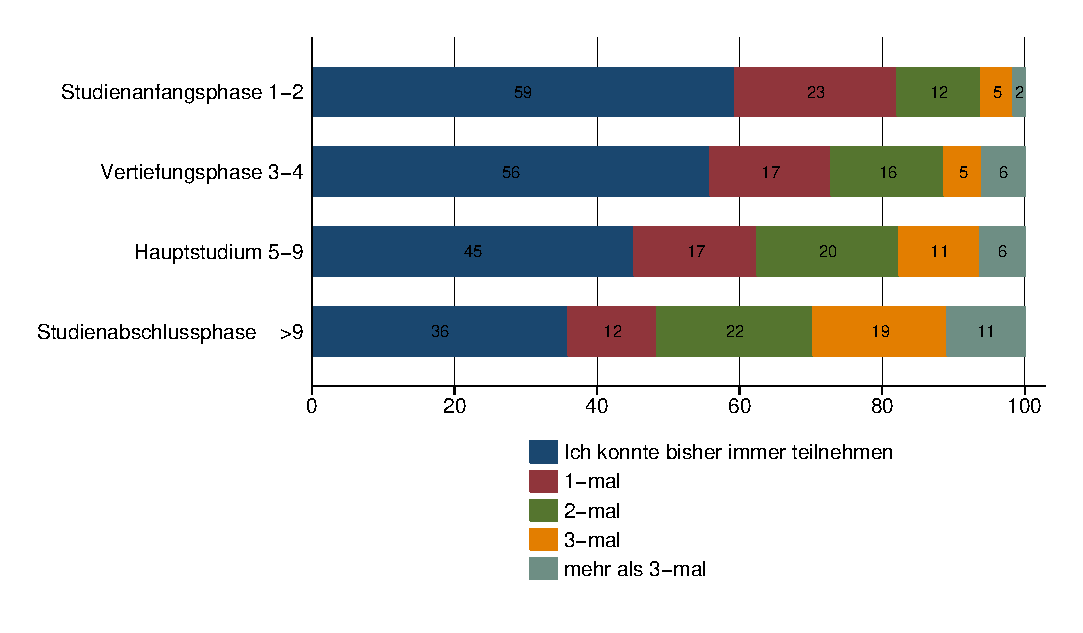
\includegraphics{image2}
    \caption{Another Sample Figure}
    \label{fig:sample2}
  \end{staticfigure}
}

\lipsum[21-40]

\end{document}
%    \end{macrocode}
%\fi
%\iffalse
%    \begin{macrocode}
%</sample-pages.tex>
%    \end{macrocode}
%\fi
%\iffalse
%    \begin{macrocode}
%<*sample-poster.tex>
%    \end{macrocode}
%\fi
%\iffalse
%    \begin{macrocode}
 % This file is public domain.

\documentclass[a0]{a0poster}

\usepackage{color}
\usepackage{mathptmx}
\usepackage{courier}
\usepackage[scaled=0.92]{helvet}
\usepackage{url}
\usepackage{flowfram}

% set up frames

\setlength{\columnsep}{2cm}

% Base the page layout on 4 column with static header.
% The static frame has height = 0.2\textheight
\NcolumnStop{4}{0.2\textheight}
% give the static frame a label to make it easier to keep track of
\setstaticframe{\value{maxstatic}}{label={title},backcolor=[cmyk]{0.64,0,0.95,0.40},textcolor=white}

% Insert a vertical line between flow frames 2 and 3:
\insertvrule{flow}{2}{flow}{3}

% On the first page, replace last two columns with
% 2 columns and a static underneath
\setflowframe{3,4}{pages={>1}}

\computeflowframearea{3,4}
\twocolumnSbottominarea[1]{0.5\ffareaheight}{\ffareawidth}{\ffareaheight}{\ffareax}{\ffareay}
\setstaticframe{\value{maxstatic}}{label={info},backcolor=[cmyk]{0.26,0,0.76,0},clear}

% insert a horizontal rule between flow frame 5 and static
% frame 5
\inserthrule*[0.5\columnsep]{flow}{5}{static}{info}

\setallflowframes{backcolor=[cmyk]{0.15,0,0.69,0}}

\newcommand{\sty}[1]{\textsf{#1}}
\newcommand{\env}[1]{\textsf{#1}}
\newcommand{\cmdname}[1]{\texttt{\symbol{92}#1}}
\newcommand{\meta}[1]{\textnormal{\textless\textit{#1}\textgreater}}

%\raggedright
%\setlength{\parindent}{15pt}

\begin{document}
\begin{staticcontents*}{title}
\begin{center}
\bfseries\veryHuge flowframe.sty : Creating Posters, Magazines or Brochures in \LaTeX
\vskip1cm
\huge Nicola L. C. Talbot
\vskip2ex
\normalsize \url{http://www.dickimaw-books.com/}
\end{center}
\end{staticcontents*}

\pagestyle{empty}

\begin{staticcontents*}{info}
\begin{staticfigure}

\begin{verbatim}
    % Make the distance between columns = 1.5cm
    \setlength{\columnsep}{2cm}

    % Make a 4 column layout with a static frame on top.
    % The static frame has height = 0.2\textheight
    \NcolumnStop{4}{0.2\textheight}

    % give the static frame a label to make it easier to keep track of
    \setstaticframe{\value{maxstatic}}{label={title},backcolor=[cmyk]{0.64,0,0.95,0.40},textcolor=white}

    % On the first page, replace the 3rd and 4th columns
    % with two shorter columns with a static frame underneath
    \setflowframe{3,4}{pages={>1}}

    % The area taken up by the 3rd and 4th columns is given by
    \computeflowframearea{3,4}
    
    % Set up new frames in this area
    \twocolumnSbottominarea[1]{0.5}{\ffareawidth}{\ffareaheight}{\ffareax}{\ffareay}

    % Assign a label to the last static frame to be created, and set background colour
    \setstaticframe{\value{maxstatic}}{label={info},backcolor=[cmyk]{0.26,0,0.76,0}}

    % Set the background colour for all flow frames
    \setallflowframes{backcolor=[cmyk]{0.15,0,0.69,0}}
\end{verbatim}

\caption{The commands used to define the frames for this document}
\protect\label{fig:thisdoc}
\end{staticfigure}
\end{staticcontents*}

This is a modified version of the manual for the \sty{flowfram} 
package.  It is intended to illustrated what can be done. See the 
full manual (ffuserguide.pdf) for
a comprehensive description, as this may now be out of date. The commands used to define the frames for
this document are shown in Figure~\ref{fig:thisdoc}.
If the columns are very narrow, it may be better to
use \cmdname{raggedright}, otherwise \TeX\ may have a
problem working out the line breaks.

\section{Introduction}

The \sty{flowfram} package is designed to enable you to create
frames in a document such that the 
contents of the \env{document} environment flow from one 
frame to the next in the order that they were defined.  
This is useful for creating posters
or magazines or any other form of document that does not 
conform to the standard one or two column layout.

\section{Setting up Frames}

The \sty{flowfram} package provides three types of frame:
{flow frames}, {static 
frames} and {dynamic frames}.

\subsection{Flow Frames}

The flow frame is the principle type of frame.
The text of the \env{document} environment will flow from 
one frame to the next in order of definition. Each 
flow frame has an associated width, height, 
position on the page, and optionally a border.

It is recommended that all the flow frames in a document
have the same width, otherwise problems may occur
when a paragraph spans to flow frames of unequal
widths. This is because \TeX's output routine does not
register the change in \cmdname{hsize} until it reaches
a paragraph break. If it is absolutely necessary for 
flow frames to have unequal widths, judicious use of
\cmdname{framebreak} is required.

\subsection{Static Frames}

A static frame is a rectangular area in which text neither
flows into, nor flows out of.  The contents must be set
explicitly, and once set, the contents of the static frame will
remain the same on each page until it is explicitly 
changed.  Thus, a static frame can be used, for example, to make 
a company logo appear in the same place on every page.

\subsection{Dynamic Frames}

A dynamic frame is similar to a static frame, but its contents
are re-typeset on each page. (A static frame stores its 
contents in a savebox, whereas a dynamic frame stores its
contents in a macro).

\section{Frame Attributes}
\label{sec:modattr}

Once you have defined the {flow frames}, {static frames} and 
{dynamic frames}, their attributes can be changed. 
The three types of frame mostly have the 
same set of attributes, but some are specific to a certain type.
The available attributes are as follows
(\textsuperscript{\textbf{F}} indicates the key is
only available for {flow frames}, 
\textsuperscript{\textbf{S}} indicates the key is only available 
for {static frames}
and \textsuperscript{\textbf{D}} indicates the key
is only available for {dynamic frames}):

\begin{description}
\item[width=\meta{length}]  The width of the frame.

\item[height=\meta{length}] The height of the frame.

\item[x=\meta{length}] The x-coordinate of the frame.

\item[y=\meta{length}] The y-coordinate of the frame.

\item[border=\meta{style}] The style of the border around the 
frame, this can take the values: \texttt{none} (no border),
\texttt{plain} (plain border) or the name of a \LaTeX\ 
frame making command without the preceding backslash. 
The value \texttt{fbox} is equivalent to \texttt{plain}.

\item[offset=\meta{offset}] The border offset, if it is a 
user-defined border.  This is the distance from the outer
edge of the left hand border to the left edge of the
bounding box of the text inside the border.  The \sty{flowfram}
package is able to compute the border for 
known frame making commands. 
If you define your own frame making command, you may need to 
specify the offset explicitly, or the frames 
may end up shifted to the right or left.

\item[bordercolor=\meta{colour}] The colour of the border
if you are using a standard frame making command.
The colour can either be specified as, e.g.\ \texttt{green},
or including the colour model, e.g. \verb/[rgb]{0,1,0}/.

\item[textcolor=\meta{colour}] The text colour for that 
frame. Again, the colour can either be specified as, 
e.g.\ \texttt{green}, or including the colour model, 
e.g. \verb/[rgb]{0,1,0}/.

\item[pages=\meta{page list}] The {list of 
pages} for which the frame
should appear. This can either have the values: \texttt{all},
\texttt{even}, \texttt{odd} or \texttt{none} (the latter 
removes the frame from that point on---useful if you
have multiple pages with the same number), or it can be a 
comma-separated list of single pages, or 
{page ranges}.

\item[margin=\meta{side}\textsuperscript{F}] The side of
the flow frame that its corresponding margin should go on. This
can take the values \texttt{left} or \texttt{right}.

\item[clear=\meta{boolean}\textsuperscript{S}] If this value
is set, the static frame will be cleared at the start of the
next page.

\item[style=\meta{cmd}\textsuperscript{D}] This should be
the name of a command \emph{without} the preceding backslash, 
to be applied to the contents of the specified dynamic frame. 
The command may either be a declaration, for example \verb/style=large/
which will set the contents of all the dynamic frames in a
large font, or it can be a command that takes a single argument,
for example \verb/style=textbf/
which will make the text for all the dynamic frames come out in 
bold.  To unset a style, do \verb/style=none/.

\end{description}

\section{Miscellaneous}

\subsection{Page Layout}

The \sty{flowfram} package has the package option \texttt{draft}
which will draw the {bounding boxes} for
each frame defined.  At the bottom right of each
bounding box (except for the bounding box denoting the 
typeblock), a marker will be shown to indictate the type
of frame, its IDN and its IDL.

You can see the layout for the current page (irrespective of
whether or not the \texttt{draft} option has been set) using
the command:\newline 
\cmdname{flowframeshowlayout}

The headers and footers will appear as usual (but will not
be shown in draft mode), according to the format given by 
\cmdname{pagestyle}.

\subsection{Frame Stacking Order}

The material on each page is placed in the following order:
\begin{enumerate}
\item Each static frame defined for that page in ascending
order of IDN.

\item Each flow frame defined for that page in ascending
order of IDN.

\item Each dynamic frame defined for that page in ascending
order of IDN.

\item {Bounding boxes} if the \texttt{draft}
package option has been used.
\end{enumerate}

This ordering can be used to determine if you want something
to overlay or underlay everything else on the page. 

\subsection{Prematurely Ending a Flow Frame}

You can force text to move immediately to the next defined
flow frame using one of the standard \LaTeX\ page breaking commands
which  work in an analogous way to the way they
work in standard two column mode. 

The command \cmdname{framebreak} is provided for situations
where a paragraph spans two flow frames
of different widths, as \TeX's output routine does not 
adjust to the new value of \cmdname{hsize} until the last 
paragraph of the previous frame has ended. As a 
result, the end of the paragraph at the beginning of the new
flow frame retains the width of the previous flow frame.

If you want to start a new page, rather than simply move to the 
next frame, use the command\newline
\cmdname{finishthispage}.

\subsection{Floats}

Since floats (such as figures and tables) can only go in 
{flow frames}, this package provides
the additional environments: 
\env{staticfigure} and  
\env{statictable} which can be used in static frames
and dynamic frames. Unlike their \env{figure} and
\env{table} counterparts, they are fixed in place, and
so do not take an optional placement specifier. The 
\cmdname{caption} and \cmdname{label} commands can 
be used within \env{staticfigure} and \env{statictable} as
usual.

The standard \env{figure} and \env{table} commands will 
behave as usual in the flow frames, but their starred versions,
\env{figure*} and \env{table*} behave no differently
from \env{figure} and \env{table}.

\subsection{Global Values}

The following macros can be changed using \cmdname{renewcommand}:

\begin{itemize}
\item \cmdname{setffdraftcolor} 

This sets the colour of the bounding box
when it is displayed in draft mode.

\item 
\cmdname{setffdrafttypeblockcolor} 

This sets the colour of
the bounding box of the typeblock when it is displayed
in draft mode.

\item \cmdname{fflabelfont}

This sets the font size for the bounding box markers in 
draft mode.

\end{itemize}

The following are lengths, which can be changed using
\cmdname{setlength}:

\begin{itemize}
\item \cmdname{fflabelsep}

This is the distance from the right hand side of the
bounding box at which to place the bounding box marker.

\item \cmdname{flowframesep}

This is the gap between the text of the frame and
its border, for the standard border types. 

\item \cmdname{flowframerule}

This is the width of the frame's border, if using
a border given by a frame making command that uses \cmdname{fboxsep}
to set its border width.

\item \cmdname{columnsep}

This is the horizontal distance between flow frames when using one of the
\cmdname{Ncolumn} type of commands

\item \cmdname{vcolumnsep}

This is the vertical distance between the flow frames and the static or
dynamic frame when using one of the \cmdname{Ncolumntop} type of commands.
\end{itemize}

\end{document}
%    \end{macrocode}
%\fi
%\iffalse
%    \begin{macrocode}
%</sample-poster.tex>
%    \end{macrocode}
%\fi
%\iffalse
%    \begin{macrocode}
%<*sample-rot.tex>
%    \end{macrocode}
%\fi
%\iffalse
%    \begin{macrocode}
 % This file is public domain.

\documentclass[a4paper]{article}

\usepackage[draft]{flowfram}
\usepackage{supertabular}

\newflowframe{0.3\textwidth}{0.25\textheight}{0.5\textwidth}{0.5\textheight}

\newflowframe{0.3\textwidth}{0.2\textheight}{0pt}{0.1\textheight}

\newflowframe{0.3\textwidth}{0.2\textheight}{0.5\textwidth}{0.1\textheight}

\setflowframe{1}{angle=45}
\setflowframe{3}{angle=90}

\begin{document}

This is a sample document illustrating the use of the
flowfram package. The first flow frame has been rotated
by an angle of 45 degrees. There is an asterisk in the
margin\marginpar{*}. There is also a 
footnote\footnote{down here.}.

\framebreak
\begin{supertabular}{rl}
1 & A\\
2 & B\\
3 & C\\
4 & D\\
5 & E\\
6 & F\\
7 & G\\
8 & H\\
9 & I\\
10 & J\\
11 & K\\
12 & L\\
13 & M\\
14 & N\\
15 & O\\
16 & P\\
17 & Q\\
18 & R\\
19 & S\\
20 & T\\
\end{supertabular}

\end{document}
%    \end{macrocode}
%\fi
%\iffalse
%    \begin{macrocode}
%</sample-rot.tex>
%    \end{macrocode}
%\fi
%\iffalse
%    \begin{macrocode}
%<*sample.tex>
%    \end{macrocode}
%\fi
%\iffalse
%    \begin{macrocode}
 % This file is public domain.

\documentclass[a4paper,twoside]{book}

\usepackage{times}
\usepackage{courier}
\usepackage{helvet}
\usepackage[margin=1in,top=1in,bottom=1in]{geometry}
\usepackage[colorlinks,
            linkcolor=black,
            urlcolor=black,
            plainpages=false,
            pdfpagelabels=true]{hyperref}
\usepackage{fancybox}
\usepackage{color}
\usepackage{flowfram}

\newcommand{\sty}[1]{\textsf{#1}}
\newcommand{\env}[1]{\textsf{#1}}
\newcommand{\cmdname}[1]{\texttt{\symbol{92}#1}}
\newcommand{\meta}[1]{\textnormal{\textless\textit{#1}\textgreater}}

% set up some background frames to liven up the title page
\newlength{\leftwidth}
\newlength{\rightwidth}

\computeleftedgeodd{\leftwidth}
\setlength{\leftwidth}{-\leftwidth}
\addtolength{\leftwidth}{0.4\textwidth}
\setlength{\rightwidth}{\paperwidth}
\addtolength{\rightwidth}{-\leftwidth}
% only defined on page 1 unfortunately the document
% has more than one page 1, so will need to change the settings after the title page
\vtwotone[1]{\leftwidth}{magenta}{backleft}{\rightwidth}{[cmyk]{0,0.48,0,0}}{backright}

% This is for the back cover.
\vtwotone[none]{\rightwidth}{[cmyk]{0,0.48,0,0}}{lastbackright}{\leftwidth}{magenta}{lastbackleft}

\vtwotonetop[odd]{1cm}{\leftwidth}{magenta}{oddtopleft}{\rightwidth}{[cmyk]{0,0.48,0,0}}{oddtopright}
\vtwotonetop[even]{1cm}{\rightwidth}{[cmyk]{0,0.48,0,0}}{eventopleft}{\leftwidth}{magenta}{eventopright}

% Set the margin width
\setlength{\marginparwidth}{2cm}

% now set up main document frames. Each page has a dynamic
% frame for the chapter heading, and a flow frame for the
% text.
\newflowframe{0.6\textwidth}{\textheight}{0pt}{0pt}[main]
\newdynamicframe{0.38\textwidth}{\textheight}{0.62\textwidth}{0pt}[chaphead]

% swap them round on even pages
\setflowframe*{main}{evenx=0.4\textwidth}
\setdynamicframe*{chaphead}{evenx=0pt}

% set the margins to appear on the spine side of the page
\setflowframe*{main}{margin=inner}

% put chapter headings in dynamic frame with IDL chaphead
\dfchaphead*{chaphead}

% append chapter minitocs to same dynamic frame.
\appenddfminitoc*{chaphead}

% change the style of the chapter headings

% numbered chapters:
\renewcommand{\DFchapterstyle}[1]{%
\raggedright\sffamily\bfseries\Huge\color{blue}#1\par
}

% unnumbered chapters:
\renewcommand{\DFschapterstyle}[1]{\raggedright\sffamily\bfseries\Huge\color{blue} #1\par
}

% Make thumb tabs (specify each tab to be 2in high)

\makethumbtabs{2in}
\enableminitoc

% Thumbtabs are grey by default which looks a bit boring,
% so change the colours
\setthumbtab{1}{backcolor=[rgb]{0.15,0.15,1}}
\setthumbtab{2}{backcolor=[rgb]{0.2,0.2,1}}
\setthumbtab{3}{backcolor=[rgb]{0.25,0.25,1}}
\setthumbtab{4}{backcolor=[rgb]{0.3,0.3,1}}

% change the text style on the thumbtabs
%\newcommand{\thumbtabstyle}[1]{\textbf{\sffamily\large #1}}
\newcommand{\thumbtabstyle}[1]{\textsc{\sffamily #1}}
\setthumbtab{all}{style=thumbtabstyle,textcolor=white}

% set default page style

\pagestyle{plain}

% Put headers and footers in dynamic frames
\makedfheaderfooter

\newlength{\xoffset}
\computerightedgeodd{\xoffset}
\addtolength{\xoffset}{-2cm}
\newlength{\yoffset}
\computebottomedge{\yoffset}

\newcommand{\footstyle}[1]{\bfseries\LARGE #1}

% pages is initially set to none, as I don't want the footer to
% appear on the title page.

\setdynamicframe*{footer}{oddx=\xoffset,y=\yoffset,width=2cm,height=2cm,
backcolor=blue,textcolor=white,style=footstyle,pages=none}

% now work out the x offset for the even pages

\computeleftedgeeven{\xoffset}
\setdynamicframe*{footer}{evenx=\xoffset}

\begin{document}
\ffswapoddeven*{main}% swap odd and even position of frame for the title page
\dfswapoddeven*{chaphead}
\title{Creating Flow Frames for Posters or Magazines}
\author{Nicola L. C. Talbot\\[1cm]\url{http://www.dickimaw-books.com/}}
\date{}
\pagenumbering{alph}
\maketitle

% make table of contents appear on a right hand page
\cleardoublepage
%suppress the background
\setstaticframe*{backleft}{pages=none}
\setstaticframe*{backright}{pages=none}

\frontmatter
%\tableofcontents
\tocandthumbtabindex
% make the footers appear from this point on
\setdynamicframe*{footer}{pages=all}

\clearpage
\dfswapoddeven*{chaphead}
\ffswapoddeven*{main}% swap back again

\mainmatter
\chapter{Introduction}
\enablethumbtabs
\pagenumbering{arabic}

The \sty{flowfram} package is designed to enable you to create
frames in a document such that the 
contents of the \env{document} environment flow from one 
frame to the next in the order that they were defined.  
This is useful for creating posters\marginpar{A marginal note}
or magazines or any other form of document that does not 
conform to the standard one or two column layout.

This document has \themaxflow\ flow 
\ifthenelse{\value{maxflow}=1}{frame}{frames}, \themaxstatic\ static
\ifthenelse{\value{maxstatic}=1}{frame}{frames} and 
\themaxdynamic\ dynamic \ifthenelse{\value{maxdynamic}=1}{frame}{frames}.

\chapter{Setting up Frames}

The \sty{flowfram} package provides three types of frame:
{flow frames}, {static 
frames} and {dynamic frames}.

\section{Flow Frames}

The flow frame is the principle type of frame.
The text of the \env{document} environment will flow from 
one frame to the next in order of definition. Each 
flow frame has an associated width, height, 
position on the page, and optionally a border\footnote{A
footnote!}.

\section{Static Frames}

A static frame is a rectangular area in which text neither
flows into, nor flows out of.  The contents must be set
explicitly, and once set, the contents of the static frame will
remain the same on each page until it is explicitly 
changed.  Thus, a static frame can be used, for example, to make 
a company logo appear in the same place on every page.

\section{Dynamic Frames}

A dynamic frame is similar to a static frame, but its contents
are re-typeset on each page. (A static frame stores its 
contents in a savebox, whereas a dynamic frame stores its
contents in a macro).

\chapter{Frame Attributes}
\label{sec:modattr}

Once you have defined the {flow frames}, {static frames} and 
{dynamic frames}, their attributes can be changed. 
The three types of frame mostly have the 
same set of attributes, but some are specific to a certain type.
The available attributes are as follows
(\textsuperscript{\textbf{F}} indicates the key is
only available for {flow frames}, 
\textsuperscript{\textbf{S}} indicates the key is only available 
for {static frames}
and \textsuperscript{\textbf{D}} indicates the key
is only available for {dynamic frames}):

\begin{description}
\item[width=\meta{length}]  The width of the frame.

\item[height=\meta{length}] The height of the frame.

\item[x=\meta{length}] The x-coordinate of the frame.

\item[y=\meta{length}] The y-coordinate of the frame.

\item[border=\meta{style}] The style of the border around the 
frame, this can take the values: \texttt{none} (no border),
\texttt{plain} (plain border) or the name of a \LaTeX\ 
frame making command without the preceding backslash. 
The value \texttt{fbox} is equivalent to \texttt{plain}.

\item[offset=\meta{offset}] The border offset, if it is a 
user-defined border.  This is the distance from the outer
edge of the left hand border to the left edge of the
bounding box of the text inside the border.  The \sty{flowfram}
package is able to compute the border for 
known frame making commands. 
If you define your own frame making command, you may need to 
specify the offset explicitly, or the frames 
may end up shifted to the right or left.

\item[bordercolor=\meta{colour}] The colour of the border
if you are using a standard frame making command.
The colour can either be specified as, e.g.\ \texttt{green},
or including the colour model, e.g. \verb/[rgb]{0,1,0}/.

\item[textcolor=\meta{colour}] The text colour for that 
frame. Again, the colour can either be specified as, 
e.g.\ \texttt{green}, or including the colour model, 
e.g. \verb/[rgb]{0,1,0}/.

\item[pages=\meta{page list}] The {list of 
pages} for which the frame
should appear. This can either have the values: \texttt{all},
\texttt{even}, \texttt{odd} or \texttt{none} (the latter 
removes the frame from that point on---useful if you
have multiple pages with the same number), or it can be a 
comma-separated list of single pages, or 
{page ranges}.

\item[margin=\meta{side}\textsuperscript{F}] The side of
the flow frame that its corresponding margin should go on. This
can take the values \texttt{left} or \texttt{right}.

\item[clear=\meta{boolean}\textsuperscript{S}] If this value
is set, the static frame will be cleared at the start of the
next page.

\item[style=\meta{cmd}\textsuperscript{D}] This should be
the name of a command \emph{without} the preceding backslash, 
to be applied to the contents of the specified dynamic frame. 
The command may either be a declaration, for example \verb/style=large/
which will set the contents of all the dynamic frames in a
large font, or it can be a command that takes a single argument,
for example \verb/style=textbf/
which will make the text for all the dynamic frames come out in 
bold.  To unset a style, do \verb/style=none/.

\end{description}

\chapter{Miscellaneous}

\section{Page Layout}

The \sty{flowfram} package has the package option \texttt{draft}
which will draw the {bounding boxes} for
each frame defined.  At the bottom right of each
bounding box (except for the bounding box denoting the 
typeblock), a marker will be shown to indictate the type
of frame, its IDN and its IDL.

You can see the layout for the current page (irrespective of
whether or not the \texttt{draft} option has been set) using
the command:\newline 
\cmdname{flowframeshowlayout}

The headers and footers will appear as usual (but will not
be shown in draft mode), according to the format given by 
\cmdname{pagestyle}.

\section{Frame Stacking Order}

The material on each page is placed in the following order:
\begin{enumerate}
\item Each static frame defined for that page in ascending
order of IDN.

\item Each flow frame defined for that page in ascending
order of IDN.

\item Each dynamic frame defined for that page in ascending
order of IDN.

\item {Bounding boxes} if the \texttt{draft}
package option has been used.
\end{enumerate}

This ordering can be used to determine if you want something
to overlay or underlay everything else on the page. 

\section{Prematurely Ending a Flow Frame}

You can force text to move immediately to the next defined
flow frame using one of the standard \LaTeX\ page breaking commands
which  work in an analogous way to the way they
work in standard two column mode. 

The command \cmdname{framebreak} is provided for situations
where a paragraph spans two flow frames
of different widths, as \TeX's output routine does not 
adjust to the new value of \cmdname{hsize} until the last 
paragraph of the previous frame has ended. As a 
result, the end of the paragraph at the beginning of the new
flow frame retains the width of the previous flow frame.

If you want to start a new page, rather than simply move to the 
next frame, use the command\newline
\cmdname{finishthispage}.

\section{Floats}

Since floats (such as figures and tables) can only go in 
{flow frames}, this package provides
the additional environments: 
\env{staticfigure} and  
\env{statictable} which can be used in static frames
and dynamic frames. Unlike their \env{figure} and
\env{table} counterparts, they are fixed in place, and
so do not take an optional placement specifier. The 
\cmdname{caption} and \cmdname{label} commands can 
be used within \env{staticfigure} and \env{statictable} as
usual.

The standard \env{figure} and \env{table} commands will 
behave as usual in the flow frames, but their starred versions,
\env{figure*} and \env{table*} behave no differently
from \env{figure} and \env{table}.

\section{Global Values}

The following macros can be changed using \cmdname{renewcommand}:

\begin{itemize}
\item \cmdname{setffdraftcolor} 

This sets the colour of the bounding box
when it is displayed in draft mode.

\item 
\cmdname{setffdrafttypeblockcolor} 

This sets the colour of
the bounding box of the typeblock when it is displayed
in draft mode.

\item \cmdname{fflabelfont}

This sets the font size for the bounding box markers in 
draft mode.

\end{itemize}

The following are lengths, which can be changed using
\cmdname{setlength}:
\marginpar{Another marginal note}

\begin{itemize}
\item \cmdname{fflabelsep}

This is the distance from the right hand side of the
bounding box at which to place the bounding box marker.

\item \cmdname{flowframesep}

This is the gap between the text of the frame and
its border, for the standard border types. 

\item \cmdname{flowframerule}

This is the width of the frame's border, if using
a border given by a frame making command that uses \cmdname{fboxsep}
to set its border width.
\end{itemize}


\chapter*{Contact Details}
\disablethumbtabs

Dr Nicola Talbot\\
School of Computing Sciences\\
University of East Anglia\\
Norwich. Norfolk. NR4 7TJ. UK\\
\url{http://theoval.cmp.uea.ac.uk/~nlct/}

\finishthispage\mbox{}
\setdynamiccontents*{chaphead}{}
\setdynamicframe*{footer}{pages=none}
\setstaticframe*{lastbackleft,lastbackright}{pages=even}
\end{document}
%    \end{macrocode}
%\fi
%\iffalse
%    \begin{macrocode}
%</sample.tex>
%    \end{macrocode}
%\fi
%\iffalse
%    \begin{macrocode}
%<*sample1.tex>
%    \end{macrocode}
%\fi
%\iffalse
%    \begin{macrocode}
 % This file is public domain.

\documentclass[a4paper]{article}

\usepackage[a4paper,landscape,margin=1in]{geometry}
\usepackage{fancybox}
\usepackage{color}
\usepackage{flowfram}

\showframebboxtrue
\showtypeblocktrue

% set up frames

% Base the page layout on 4 column with static header
\NcolumnStop{4}{1in}

% On the first page, replace last two columns with
% 2 columns and a static underneath
\setflowframe{3,4}{pages={>1}}
\twocolumnSbottominarea[1]{1in}{0.5\textwidth}{\flowframeheight{3}}{0.5\textwidth}{0pt}

\begin{staticcontents}{2}
The page layout for this document was obtained with
the following commands:
\begin{verbatim}
\NcolumnStop{4}{1in}
\setflowframe{3,4}{pages={>1}}
\twocolumnSbottominarea[1]{1in}{0.5\textwidth}{flowframeheight{3}}
{0.5\textwidth}{0pt}
\end{verbatim}
\end{staticcontents}

\newcommand{\sty}[1]{\textsf{#1}}
\newcommand{\env}[1]{\textsf{#1}}
\newcommand{\cmdname}[1]{\texttt{\symbol{92}#1}}
\newcommand{\meta}[1]{\textnormal{\textless\textit{#1}\textgreater}}

\raggedright
%\setlength{\parindent}{15pt}

\begin{document}

\begin{staticcontents}{1}
\title{Creating Flow Frames for Posters or Magazines}
\author{Nicola L. C. Talbot}
\date{}
\maketitle
\end{staticcontents}

This is a modified version of the manual for the \sty{flowfram} package.
It is intended to illustrated what can be done. See the full manual for
a comprehensive description.

If the columns are very narrow, it may be better to
use \cmdname{raggedright}, otherwise \TeX\ may have a
problem working out the line breaks.

\section{Introduction}

The \sty{flowfram} package is designed to enable you to create
frames in a document such that the 
contents of the \env{document} environment flow from one 
frame to the next in the order that they were defined.  
This is useful for creating posters
or magazines or any other form of document that does not 
conform to the standard one or two column layout.

\section{Setting up Frames}

The \sty{flowfram} package provides three types of frame:
{flow frames}, {static 
frames} and {dynamic frames}.

\subsection{Flow Frames}

The flow frame is the principle type of frame.
The text of the \env{document} environment will flow from 
one frame to the next in order of definition. Each 
flow frame has an associated width, height, 
position on the page, and optionally a border.

It is recommended that all the flow frames in a document
have the same width, otherwise problems may occur
when a paragraph spans to flow frames of unequal
widths. This is because \TeX's output routine does not
register the change in \cmdname{hsize} until it reaches
a paragraph break. If it is absolutely necessary for 
flow frames to have unequal widths, judicious use of
\cmdname{framebreak} is required.

\subsection{Static Frames}

A static frame is a rectangular area in which text neither
flows into, nor flows out of.  The contents must be set
explicitly, and once set, the contents of the static frame will
remain the same on each page until it is explicitly 
changed.  Thus, a static frame can be used, for example, to make 
a company logo appear in the same place on every page.

\subsection{Dynamic Frames}

A dynamic frame is similar to a static frame, but its contents
are re-typeset on each page. (A static frame stores its 
contents in a savebox, whereas a dynamic frame stores its
contents in a macro).


\section{Frame Attributes}
\label{sec:modattr}

Once you have defined the {flow frames}, {static frames} and 
{dynamic frames}, their attributes can be changed. 
The three types of frame mostly have the 
same set of attributes, but some are specific to a certain type.
The available attributes are as follows
(\textsuperscript{\textbf{F}} indicates the key is
only available for {flow frames}, 
\textsuperscript{\textbf{S}} indicates the key is only available 
for {static frames}
and \textsuperscript{\textbf{D}} indicates the key
is only available for {dynamic frames}):

\begin{description}
\item[width=\meta{length}]  The width of the frame.

\item[height=\meta{length}] The height of the frame.

\item[x=\meta{length}] The x-coordinate of the frame.

\item[y=\meta{length}] The y-coordinate of the frame.

\item[border=\meta{style}] The style of the border around the 
frame, this can take the values: \texttt{none} (no border),
\texttt{plain} (plain border) or the name of a \LaTeX\ 
frame making command without the preceding backslash. 
The value \texttt{fbox} is equivalent to \texttt{plain}.

\item[offset=\meta{offset}] The border offset, if it is a 
user-defined border.  This is the distance from the outer
edge of the left hand border to the left edge of the
bounding box of the text inside the border.  The \sty{flowfram}
package is able to compute the border for 
known frame making commands. 
If you define your own frame making command, you may need to 
specify the offset explicitly, or the frames 
may end up shifted to the right or left.

\item[bordercolor=\meta{colour}] The colour of the border
if you are using a standard frame making command.
The colour can either be specified as, e.g.\ \texttt{green},
or including the colour model, e.g. \verb/[rgb]{0,1,0}/.

\item[textcolor=\meta{colour}] The text colour for that 
frame. Again, the colour can either be specified as, 
e.g.\ \texttt{green}, or including the colour model, 
e.g. \verb/[rgb]{0,1,0}/.

\item[pages=\meta{page list}] The {list of 
pages} for which the frame
should appear. This can either have the values: \texttt{all},
\texttt{even}, \texttt{odd} or \texttt{none} (the latter 
removes the frame from that point on---useful if you
have multiple pages with the same number), or it can be a 
comma-separated list of single pages, or 
{page ranges}.

\item[margin=\meta{side}\textsuperscript{F}] The side of
the flow frame that its corresponding margin should go on. This
can take the values \texttt{left} or \texttt{right}.

\item[clear=\meta{boolean}\textsuperscript{S}] If this value
is set, the static frame will be cleared at the start of the
next page.

\item[style=\meta{cmd}\textsuperscript{D}] This should be
the name of a command \emph{without} the preceding backslash, 
to be applied to the contents of the specified dynamic frame. 
The command may either be a declaration, for example \verb/style=large/
which will set the contents of all the dynamic frames in a
large font, or it can be a command that takes a single argument,
for example \verb/style=textbf/
which will make the text for all the dynamic frames come out in 
bold.  To unset a style, do \verb/style=none/.

\end{description}

\section{Miscellaneous}

\subsection{Page Layout}

The \sty{flowfram} package has the package option \texttt{draft}
which will draw the {bounding boxes} for
each frame defined.  At the bottom right of each
bounding box (except for the bounding box denoting the 
typeblock), a marker will be shown to indictate the type
of frame, its IDN and its IDL.

You can see the layout for the current page (irrespective of
whether or not the \texttt{draft} option has been set) using
the command:\newline 
\cmdname{flowframeshowlayout}

The headers and footers will appear as usual (but will not
be shown in draft mode), according to the format given by 
\cmdname{pagestyle}.

\subsection{Frame Stacking Order}

The material on each page is placed in the following order:
\begin{enumerate}
\item Each static frame defined for that page in ascending
order of IDN.

\item Each flow frame defined for that page in ascending
order of IDN.

\item Each dynamic frame defined for that page in ascending
order of IDN.

\item {Bounding boxes} if the \texttt{draft}
package option has been used.
\end{enumerate}

This ordering can be used to determine if you want something
to overlay or underlay everything else on the page. 

\subsection{Prematurely Ending a Flow Frame}

You can force text to move immediately to the next defined
flow frame using one of the standard \LaTeX\ page breaking commands
which  work in an analogous way to the way they
work in standard two column mode. 

The command \cmdname{framebreak} is provided for situations
where a paragraph spans two flow frames
of different widths, as \TeX's output routine does not 
adjust to the new value of \cmdname{hsize} until the last 
paragraph of the previous frame has ended. As a 
result, the end of the paragraph at the beginning of the new
flow frame retains the width of the previous flow frame.

If you want to start a new page, rather than simply move to the 
next frame, use the command\newline
\cmdname{finishthispage}.

\subsection{Floats}

Since floats (such as figures and tables) can only go in 
{flow frames}, this package provides
the additional environments: 
\env{staticfigure} and  
\env{statictable} which can be used in static frames
and dynamic frames. Unlike their \env{figure} and
\env{table} counterparts, they are fixed in place, and
so do not take an optional placement specifier. The 
\cmdname{caption} and \cmdname{label} commands can 
be used within \env{staticfigure} and \env{statictable} as
usual.

The standard \env{figure} and \env{table} commands will 
behave as usual in the flow frames, but their starred versions,
\env{figure*} and \env{table*} behave no differently
from \env{figure} and \env{table}.

\subsection{Global Values}

The following macros can be changed using \cmdname{renewcommand}:

\begin{itemize}
\item \cmdname{setffdraftcolor} 

This sets the colour of the bounding box
when it is displayed in draft mode.

\item 
\cmdname{setffdrafttypeblockcolor} 

This sets the colour of
the bounding box of the typeblock when it is displayed
in draft mode.

\item \cmdname{fflabelfont}

This sets the font size for the bounding box markers in 
draft mode.

\end{itemize}

The following are lengths, which can be changed using
\cmdname{setlength}:

\begin{itemize}
\item \cmdname{fflabelsep}

This is the distance from the right hand side of the
bounding box at which to place the bounding box marker.

\item \cmdname{flowframesep}

This is the gap between the text of the frame and
its border, for the standard border types. 

\item \cmdname{flowframerule}

This is the width of the frame's border, if using
a border given by a frame making command that uses \cmdname{fboxsep}
to set its border width.
\end{itemize}

\end{document}
%    \end{macrocode}
%\fi
%\iffalse
%    \begin{macrocode}
%</sample1.tex>
%    \end{macrocode}
%\fi
%\iffalse
%    \begin{macrocode}
%<*sample2.tex>
%    \end{macrocode}
%\fi
%\iffalse
%    \begin{macrocode}
 % This file is public domain.

\documentclass[a4paper,twoside]{report}

\usepackage{url}

\newcommand{\cmdname}[1]{\texttt{\char`\\#1}}
\newcommand{\sty}[1]{\texttt{#1}}
\newcommand{\env}[1]{\texttt{#1}}
\newcommand{\meta}[1]{$\langle$\emph{#1}$\rangle$}

\begin{document}

\title{Creating Flow Frames for Posters or Magazines}
\author{Nicola L. C. Talbot\\[1cm]\url{http://www.dickimaw-books.com/}}
\date{}
\pagenumbering{alph}
\maketitle

\pagenumbering{roman}
\tableofcontents

\chapter{Introduction}
\pagenumbering{arabic}

The \sty{flowfram} package is designed to enable you to create
frames in a document such that the 
contents of the \env{document} environment flow from one 
frame to the next in the order that they were defined.  
This is useful for creating posters
or magazines or any other form of document that does not 
conform to the standard one or two column layout.

\chapter{Setting up Frames}

The \sty{flowfram} package provides three types of frame:
{flow frames}, {static 
frames} and {dynamic frames}.

\section{Flow Frames}

The flow frame is the principle type of frame.
The text of the \env{document} environment will flow from 
one frame to the next in order of definition. Each 
flow frame has an associated width, height, 
position on the page, and optionally a border.

\section{Static Frames}

A static frame is a rectangular area in which text neither
flows into, nor flows out of.  The contents must be set
explicitly, and once set, the contents of the static frame will
remain the same on each page until it is explicitly 
changed.  Thus, a static frame can be used, for example, to make 
a company logo appear in the same place on every page.

\section{Dynamic Frames}

A dynamic frame is similar to a static frame, but its contents
are re-typeset on each page. (A static frame stores its 
contents in a savebox, whereas a dynamic frame stores its
contents in a macro).

\chapter{Frame Attributes}
\label{sec:modattr}

Once you have defined the {flow frames}, {static frames} and 
{dynamic frames}, their attributes can be changed. 
The three types of frame mostly have the 
same set of attributes, but some are specific to a certain type.
The available attributes are as follows
(\textsuperscript{\textbf{F}} indicates the key is
only available for {flow frames}, 
\textsuperscript{\textbf{S}} indicates the key is only available 
for {static frames}
and \textsuperscript{\textbf{D}} indicates the key
is only available for {dynamic frames}):

\begin{description}
\item[width=\meta{length}]  The width of the frame.

\item[height=\meta{length}] The height of the frame.

\item[x=\meta{length}] The x-coordinate of the frame.

\item[y=\meta{length}] The y-coordinate of the frame.

\item[border=\meta{style}] The style of the border around the 
frame, this can take the values: \texttt{none} (no border),
\texttt{plain} (plain border) or the name of a \LaTeX\ 
frame making command without the preceding backslash. 
The value \texttt{fbox} is equivalent to \texttt{plain}.

\item[offset=\meta{offset}] The border offset, if it is a 
user-defined border.  This is the distance from the outer
edge of the left hand border to the left edge of the
bounding box of the text inside the border.  The \sty{flowfram}
package is able to compute the border for 
known frame making commands. 
If you define your own frame making command, you may need to 
specify the offset explicitly, or the frames 
may end up shifted to the right or left.

\item[bordercolor=\meta{colour}] The colour of the border
if you are using a standard frame making command.
The colour can either be specified as, e.g.\ \texttt{green},
or including the colour model, e.g. \verb/[rgb]{0,1,0}/.

\item[textcolor=\meta{colour}] The text colour for that 
frame. Again, the colour can either be specified as, 
e.g.\ \texttt{green}, or including the colour model, 
e.g. \verb/[rgb]{0,1,0}/.

\item[pages=\meta{page list}] The {list of 
pages} for which the frame
should appear. This can either have the values: \texttt{all},
\texttt{even}, \texttt{odd} or \texttt{none} (the latter 
removes the frame from that point on---useful if you
have multiple pages with the same number), or it can be a 
comma-separated list of single pages, or 
{page ranges}.

\item[margin=\meta{side}\textsuperscript{F}] The side of
the flow frame that its corresponding margin should go on. This
can take the values \texttt{left} or \texttt{right}.

\item[clear=\meta{boolean}\textsuperscript{S}] If this value
is set, the static frame will be cleared at the start of the
next page.

\item[style=\meta{cmd}\textsuperscript{D}] This should be
the name of a command \emph{without} the preceding backslash, 
to be applied to the contents of the specified dynamic frame. 
The command may either be a declaration, for example \verb/style=large/
which will set the contents of all the dynamic frames in a
large font, or it can be a command that takes a single argument,
for example \verb/style=textbf/
which will make the text for all the dynamic frames come out in 
bold.  To unset a style, do \verb/style=none/.

\end{description}

\chapter{Miscellaneous}

\section{Page Layout}

The \sty{flowfram} package has the package option \texttt{draft}
which will draw the {bounding boxes} for
each frame defined.  At the bottom right of each
bounding box (except for the bounding box denoting the 
typeblock), a marker will be shown to indictate the type
of frame, its IDN and its IDL.

You can see the layout for the current page (irrespective of
whether or not the \texttt{draft} option has been set) using
the command:\newline 
\cmdname{flowframeshowlayout}

The headers and footers will appear as usual (but will not
be shown in draft mode), according to the format given by 
\cmdname{pagestyle}.

\section{Frame Stacking Order}

The material on each page is placed in the following order:
\begin{enumerate}
\item Each static frame defined for that page in ascending
order of IDN.

\item Each flow frame defined for that page in ascending
order of IDN.

\item Each dynamic frame defined for that page in ascending
order of IDN.

\item {Bounding boxes} if the \texttt{draft}
package option has been used.
\end{enumerate}

This ordering can be used to determine if you want something
to overlay or underlay everything else on the page. 

\section{Prematurely Ending a Flow Frame}

You can force text to move immediately to the next defined
flow frame using one of the standard \LaTeX\ page breaking commands
which  work in an analogous way to the way they
work in standard two column mode. 

The command \cmdname{framebreak} is provided for situations
where a paragraph spans two flow frames
of different widths, as \TeX's output routine does not 
adjust to the new value of \cmdname{hsize} until the last 
paragraph of the previous frame has ended. As a 
result, the end of the paragraph at the beginning of the new
flow frame retains the width of the previous flow frame.

If you want to start a new page, rather than simply move to the 
next frame, use the command\newline
\cmdname{finishthispage}.

\section{Floats}

Since floats (such as figures and tables) can only go in 
{flow frames}, this package provides
the additional environments: 
\env{staticfigure} and  
\env{statictable} which can be used in static frames
and dynamic frames. Unlike their \env{figure} and
\env{table} counterparts, they are fixed in place, and
so do not take an optional placement specifier. The 
\cmdname{caption} and \cmdname{label} commands can 
be used within \env{staticfigure} and \env{statictable} as
usual.

The standard \env{figure} and \env{table} commands will 
behave as usual in the flow frames, but their starred versions,
\env{figure*} and \env{table*} behave no differently
from \env{figure} and \env{table}.

\section{Global Values}

The following macros can be changed using \cmdname{renewcommand}:

\begin{itemize}
\item \cmdname{setffdraftcolor} 

This sets the colour of the bounding box
when it is displayed in draft mode.

\item 
\cmdname{setffdrafttypeblockcolor} 

This sets the colour of
the bounding box of the typeblock when it is displayed
in draft mode.

\item \cmdname{fflabelfont}

This sets the font size for the bounding box markers in 
draft mode.

\end{itemize}

The following are lengths, which can be changed using
\cmdname{setlength}:

\begin{itemize}
\item \cmdname{fflabelsep}

This is the distance from the right hand side of the
bounding box at which to place the bounding box marker.

\item \cmdname{flowframesep}

This is the gap between the text of the frame and
its border, for the standard border types. 

\item \cmdname{flowframerule}

This is the width of the frame's border, if using
a border given by a frame making command that uses \cmdname{fboxsep}
to set its border width.
\end{itemize}


\chapter*{Contact Details}

Dr Nicola Talbot\\
Dickimaw Books\\
\url{http://www.dickimaw-books.com/}

\end{document}
%    \end{macrocode}
%\fi
%\iffalse
%    \begin{macrocode}
%</sample2.tex>
%    \end{macrocode}
%\fi
%\iffalse
%    \begin{macrocode}
%<*sample3.tex>
%    \end{macrocode}
%\fi
%\iffalse
%    \begin{macrocode}
 % This file is public domain.

\documentclass{article}

\usepackage{color}
\usepackage[draft]{flowfram}
\usepackage{tikz}
\usetikzlibrary{snakes}

\newstaticframe[1,2]{3in}{3in}{0pt}{0pt}[sf1]
\newdynamicframe[1,3]{2in}{3in}{0.5\textwidth}{0.5\textheight}[df1]

\newstaticframe[2]{3in}{3in}{0.5\textwidth}{0.5\textheight}[sf2]

\newdynamicframe[3]{2in}{2in}{0.5\textwidth}{0pt}[df2]

\setlength{\sdfparindent}{\parindent}

\onecolumn

\newlength\fancywidth
\newlength\fancyheight
\newlength\fancydepth

\newcommand{\fancyframe}[1]{%
\settowidth{\fancywidth}{#1}%
\settoheight{\fancyheight}{#1}%
\settodepth{\fancydepth}{#1}%
\addtolength{\fancyheight}{\fancydepth}%
\hspace{-\flowframesep}%
\tikz[baseline=0pt]{%
\draw[snake=bumps,raise snake=\flowframesep,line width=\flowframerule]
  (0pt,0pt)
  rectangle (\fancywidth,\fancyheight);
}}

\begin{document}
\setstaticframe{1,2}{valign=t}
\setstaticframe{1}{border=fancyframe}
\setstaticcontents{1}{Top\par
\vfill
Bottom}

%\setdynamiccontents{1}{Bar}
%\begin{dynamiccontents*}{df1}
%Paragraph 1
%
%Paragraph 2
%\end{dynamiccontents*}

\mbox{}

\newpage\mbox{}

\begin{staticcontents*}{sf1}
Some text on the left static frame.
\continueonframe[continued \relativeframelocation{static}{2}{static}{1}]{sf2}
Some more text on the right static frame, and
some more text to pad it out a bit.
\end{staticcontents*}

\newpage\mbox{}

\begin{dynamiccontents}{1}
Some text in the first dynamic frame.
\continueonframe[continued \reldynamicloc*{df2}{df1}]{2}
Some more text in the second dynamic frame, and
some more text to pad it out a bit.
\end{dynamiccontents}

\end{document}
%    \end{macrocode}
%\fi
%\iffalse
%    \begin{macrocode}
%</sample3.tex>
%    \end{macrocode}
%\fi
%\iffalse
%    \begin{macrocode}
%<*sampleRL.tex>
%    \end{macrocode}
%\fi
%\iffalse
%    \begin{macrocode}
 % This file is public domain.

\documentclass{article}

\usepackage{lipsum}
\usepackage[RL,draft]{flowfram}

\twocolumn

\begin{document}
This is the start of the text.

\lipsum

This is the end of the text.
\end{document}
%    \end{macrocode}
%\fi
%\iffalse
%    \begin{macrocode}
%</sampleRL.tex>
%    \end{macrocode}
%\fi
%\iffalse
%    \begin{macrocode}
%<*flowfram.perl>
%    \end{macrocode}
%\fi
%\iffalse
%    \begin{macrocode}
#!/usr/bin/env perl
# File          : flowfram.perl
# Author        : Nicola L C Talbot
# Date          : 28 June 2008
# Last Modified : 1 July 2008
# Version       : 1.0
# Description   : LaTeX2HTML implementation of the flowfram package.
#                 This is not meant to emulate the flowfram package.
#                 Most of the frame related commands are ignored, to
#                 provide a simple HTML version of the document.
#
# Copyright 2007 Nicola L.C. Talbot
#
# This work may be distributed and/or modified under the
# conditions of the LaTeX Project Public License, either version 1.3
# of this license of (at your option) any later version.
# The latest version of this license is in
#   http://www.latex-project.org/lppl.txt
# and version 1.3 or later is part of all distributions of LaTeX
# version 2005/12/01 or later.
#
# This work has the LPPL maintenance status `maintained'.
#
# The Current Maintainer of this work is Nicola Talbot.

package main;

$showstaticcontents = 0;
$showdynamiccontents = 0;

sub do_cmd_onecolumninarea
{
   local($_) = @_;

   local($keyval,$pat) = &get_next_optional_argument;

   s/$next_pair_pr_rx/;''/eo;
   s/$next_pair_pr_rx/;''/eo;
   s/$next_pair_pr_rx/;''/eo;
   s/$next_pair_pr_rx/;''/eo;

   $_
}

sub do_cmd_twocolumninarea
{
   local($_) = @_;

   local($keyval,$pat) = &get_next_optional_argument;

   s/$next_pair_pr_rx/;''/eo;
   s/$next_pair_pr_rx/;''/eo;
   s/$next_pair_pr_rx/;''/eo;
   s/$next_pair_pr_rx/;''/eo;

   $_
}

sub do_cmd_Ncolumninarea
{
   local($_) = @_;

   local($keyval,$pat) = &get_next_optional_argument;

   s/$next_pair_pr_rx/;''/eo;
   s/$next_pair_pr_rx/;''/eo;
   s/$next_pair_pr_rx/;''/eo;
   s/$next_pair_pr_rx/;''/eo;
   s/$next_pair_pr_rx/;''/eo;

   $_
}

sub do_cmd_Ncolumn{
   local($_) = @_;

   local($keyval,$pat) = &get_next_optional_argument;

   s/$next_pair_pr_rx/;''/eo;

   $_
}

sub do_cmd_onecolumntopinarea
{
   local($_) = @_;

   local($keyval,$pat) = &get_next_optional_argument;

   s/$next_pair_pr_rx/;''/eo;
   s/$next_pair_pr_rx/;''/eo;
   s/$next_pair_pr_rx/;''/eo;
   s/$next_pair_pr_rx/;''/eo;
   s/$next_pair_pr_rx/;''/eo;
   s/$next_pair_pr_rx/;''/eo;

   $_
}

sub do_cmd_twocolumntopinarea
{
   local($_) = @_;

   local($keyval,$pat) = &get_next_optional_argument;

   s/$next_pair_pr_rx/;''/eo;
   s/$next_pair_pr_rx/;''/eo;
   s/$next_pair_pr_rx/;''/eo;
   s/$next_pair_pr_rx/;''/eo;
   s/$next_pair_pr_rx/;''/eo;
   s/$next_pair_pr_rx/;''/eo;

   $_
}

sub do_cmd_Ncolumntopinarea
{
   local($_) = @_;

   local($keyval,$pat) = &get_next_optional_argument;

   s/$next_pair_pr_rx/;''/eo;
   s/$next_pair_pr_rx/;''/eo;
   s/$next_pair_pr_rx/;''/eo;
   s/$next_pair_pr_rx/;''/eo;
   s/$next_pair_pr_rx/;''/eo;
   s/$next_pair_pr_rx/;''/eo;
   s/$next_pair_pr_rx/;''/eo;

   $_
}

sub do_cmd_onecolumnbottominarea
{
   local($_) = @_;

   local($keyval,$pat) = &get_next_optional_argument;

   s/$next_pair_pr_rx/;''/eo;
   s/$next_pair_pr_rx/;''/eo;
   s/$next_pair_pr_rx/;''/eo;
   s/$next_pair_pr_rx/;''/eo;
   s/$next_pair_pr_rx/;''/eo;
   s/$next_pair_pr_rx/;''/eo;

   $_
}

sub do_cmd_twocolumnbottominarea
{
   local($_) = @_;

   local($keyval,$pat) = &get_next_optional_argument;

   s/$next_pair_pr_rx/;''/eo;
   s/$next_pair_pr_rx/;''/eo;
   s/$next_pair_pr_rx/;''/eo;
   s/$next_pair_pr_rx/;''/eo;
   s/$next_pair_pr_rx/;''/eo;
   s/$next_pair_pr_rx/;''/eo;

   $_
}

sub do_cmd_Ncolumnbottominarea
{
   local($_) = @_;

   local($keyval,$pat) = &get_next_optional_argument;

   s/$next_pair_pr_rx/;''/eo;
   s/$next_pair_pr_rx/;''/eo;
   s/$next_pair_pr_rx/;''/eo;
   s/$next_pair_pr_rx/;''/eo;
   s/$next_pair_pr_rx/;''/eo;
   s/$next_pair_pr_rx/;''/eo;
   s/$next_pair_pr_rx/;''/eo;

   $_
}

sub do_cmd_onecolumnStopinarea
{
   local($_) = @_;

   local($keyval,$pat) = &get_next_optional_argument;

   s/$next_pair_pr_rx/;''/eo;
   s/$next_pair_pr_rx/;''/eo;
   s/$next_pair_pr_rx/;''/eo;
   s/$next_pair_pr_rx/;''/eo;
   s/$next_pair_pr_rx/;''/eo;

   $_
}

sub do_cmd_onecolumnDtopinarea
{
   local($_) = @_;

   local($keyval,$pat) = &get_next_optional_argument;

   s/$next_pair_pr_rx/;''/eo;
   s/$next_pair_pr_rx/;''/eo;
   s/$next_pair_pr_rx/;''/eo;
   s/$next_pair_pr_rx/;''/eo;
   s/$next_pair_pr_rx/;''/eo;

   $_
}

sub do_cmd_onecolumnSbottominarea
{
   local($_) = @_;

   local($keyval,$pat) = &get_next_optional_argument;

   s/$next_pair_pr_rx/;''/eo;
   s/$next_pair_pr_rx/;''/eo;
   s/$next_pair_pr_rx/;''/eo;
   s/$next_pair_pr_rx/;''/eo;
   s/$next_pair_pr_rx/;''/eo;

   $_
}

sub do_cmd_onecolumnDbottominarea
{
   local($_) = @_;

   local($keyval,$pat) = &get_next_optional_argument;

   s/$next_pair_pr_rx/;''/eo;
   s/$next_pair_pr_rx/;''/eo;
   s/$next_pair_pr_rx/;''/eo;
   s/$next_pair_pr_rx/;''/eo;
   s/$next_pair_pr_rx/;''/eo;

   $_
}

sub do_cmd_twocolumnStopinarea
{
   local($_) = @_;

   local($keyval,$pat) = &get_next_optional_argument;

   s/$next_pair_pr_rx/;''/eo;
   s/$next_pair_pr_rx/;''/eo;
   s/$next_pair_pr_rx/;''/eo;
   s/$next_pair_pr_rx/;''/eo;
   s/$next_pair_pr_rx/;''/eo;

   $_
}

sub do_cmd_twocolumnDtopinarea
{
   local($_) = @_;

   local($keyval,$pat) = &get_next_optional_argument;

   s/$next_pair_pr_rx/;''/eo;
   s/$next_pair_pr_rx/;''/eo;
   s/$next_pair_pr_rx/;''/eo;
   s/$next_pair_pr_rx/;''/eo;
   s/$next_pair_pr_rx/;''/eo;

   $_
}

sub do_cmd_twocolumnSbottominarea
{
   local($_) = @_;

   local($keyval,$pat) = &get_next_optional_argument;

   s/$next_pair_pr_rx/;''/eo;
   s/$next_pair_pr_rx/;''/eo;
   s/$next_pair_pr_rx/;''/eo;
   s/$next_pair_pr_rx/;''/eo;
   s/$next_pair_pr_rx/;''/eo;

   $_
}

sub do_cmd_twocolumnDbottominarea
{
   local($_) = @_;

   local($keyval,$pat) = &get_next_optional_argument;

   s/$next_pair_pr_rx/;''/eo;
   s/$next_pair_pr_rx/;''/eo;
   s/$next_pair_pr_rx/;''/eo;
   s/$next_pair_pr_rx/;''/eo;
   s/$next_pair_pr_rx/;''/eo;

   $_
}

sub do_cmd_NcolumnDbottominarea
{
   local($_) = @_;

   local($keyval,$pat) = &get_next_optional_argument;

   s/$next_pair_pr_rx/;''/eo;
   s/$next_pair_pr_rx/;''/eo;
   s/$next_pair_pr_rx/;''/eo;
   s/$next_pair_pr_rx/;''/eo;
   s/$next_pair_pr_rx/;''/eo;
   s/$next_pair_pr_rx/;''/eo;

   $_
}

sub do_cmd_NcolumnSbottominarea
{
   local($_) = @_;

   local($keyval,$pat) = &get_next_optional_argument;

   s/$next_pair_pr_rx/;''/eo;
   s/$next_pair_pr_rx/;''/eo;
   s/$next_pair_pr_rx/;''/eo;
   s/$next_pair_pr_rx/;''/eo;
   s/$next_pair_pr_rx/;''/eo;
   s/$next_pair_pr_rx/;''/eo;

   $_
}

sub do_cmd_onecolumntop
{
   local($_) = @_;

   local($keyval,$pat) = &get_next_optional_argument;

   s/$next_pair_pr_rx/;''/eo;
   s/$next_pair_pr_rx/;''/eo;

   $_
}

sub do_cmd_twocolumntop
{
   local($_) = @_;

   local($keyval,$pat) = &get_next_optional_argument;

   s/$next_pair_pr_rx/;''/eo;
   s/$next_pair_pr_rx/;''/eo;

   $_
}

sub do_cmd_Ncolumntop
{
   local($_) = @_;

   local($keyval,$pat) = &get_next_optional_argument;

   s/$next_pair_pr_rx/;''/eo;
   s/$next_pair_pr_rx/;''/eo;
   s/$next_pair_pr_rx/;''/eo;

   $_
}

sub do_cmd_onecolumnStop
{
   local($_) = @_;

   local($keyval,$pat) = &get_next_optional_argument;

   s/$next_pair_pr_rx/;''/eo;

   $_
}

sub do_cmd_twocolumnStop
{
   local($_) = @_;

   local($keyval,$pat) = &get_next_optional_argument;

   s/$next_pair_pr_rx/;''/eo;

   $_
}

sub do_cmd_NcolumnStop
{
   local($_) = @_;

   local($keyval,$pat) = &get_next_optional_argument;

   s/$next_pair_pr_rx/;''/eo;
   s/$next_pair_pr_rx/;''/eo;

   $_
}

sub do_cmd_onecolumnDtop
{
   local($_) = @_;

   local($keyval,$pat) = &get_next_optional_argument;

   s/$next_pair_pr_rx/;''/eo;

   $_
}

sub do_cmd_twocolumnDtop
{
   local($_) = @_;

   local($keyval,$pat) = &get_next_optional_argument;

   s/$next_pair_pr_rx/;''/eo;

   $_
}

sub do_cmd_NcolumnDtop
{
   local($_) = @_;

   local($keyval,$pat) = &get_next_optional_argument;

   s/$next_pair_pr_rx/;''/eo;
   s/$next_pair_pr_rx/;''/eo;

   $_
}

sub do_cmd_onecolumnbottom
{
   local($_) = @_;

   local($keyval,$pat) = &get_next_optional_argument;

   s/$next_pair_pr_rx/;''/eo;
   s/$next_pair_pr_rx/;''/eo;

   $_
}

sub do_cmd_twocolumnbottom
{
   local($_) = @_;

   local($keyval,$pat) = &get_next_optional_argument;

   s/$next_pair_pr_rx/;''/eo;
   s/$next_pair_pr_rx/;''/eo;

   $_
}

sub do_cmd_Ncolumnbottom
{
   local($_) = @_;

   local($keyval,$pat) = &get_next_optional_argument;

   s/$next_pair_pr_rx/;''/eo;
   s/$next_pair_pr_rx/;''/eo;
   s/$next_pair_pr_rx/;''/eo;

   $_
}

sub do_cmd_onecolumnSbottom
{
   local($_) = @_;

   local($keyval,$pat) = &get_next_optional_argument;

   s/$next_pair_pr_rx/;''/eo;

   $_
}

sub do_cmd_twocolumnSbottom
{
   local($_) = @_;

   local($keyval,$pat) = &get_next_optional_argument;

   s/$next_pair_pr_rx/;''/eo;

   $_
}

sub do_cmd_NcolumnSbottom
{
   local($_) = @_;

   local($keyval,$pat) = &get_next_optional_argument;

   s/$next_pair_pr_rx/;''/eo;
   s/$next_pair_pr_rx/;''/eo;

   $_
}

sub do_cmd_onecolumnDbottom
{
   local($_) = @_;

   local($keyval,$pat) = &get_next_optional_argument;

   s/$next_pair_pr_rx/;''/eo;

   $_
}

sub do_cmd_twocolumnDbottom
{
   local($_) = @_;

   local($keyval,$pat) = &get_next_optional_argument;

   s/$next_pair_pr_rx/;''/eo;

   $_
}

sub do_cmd_NcolumnDbottom
{
   local($_) = @_;

   local($keyval,$pat) = &get_next_optional_argument;

   s/$next_pair_pr_rx/;''/eo;
   s/$next_pair_pr_rx/;''/eo;

   $_
}

sub do_cmd_NcolumnDtopinarea
{
   local($_) = @_;

   local($keyval,$pat) = &get_next_optional_argument;

   s/$next_pair_pr_rx/;''/eo;
   s/$next_pair_pr_rx/;''/eo;
   s/$next_pair_pr_rx/;''/eo;
   s/$next_pair_pr_rx/;''/eo;
   s/$next_pair_pr_rx/;''/eo;
   s/$next_pair_pr_rx/;''/eo;

   $_
}

sub do_cmd_NcolumnStopinarea
{
   local($_) = @_;

   local($keyval,$pat) = &get_next_optional_argument;

   s/$next_pair_pr_rx/;''/eo;
   s/$next_pair_pr_rx/;''/eo;
   s/$next_pair_pr_rx/;''/eo;
   s/$next_pair_pr_rx/;''/eo;
   s/$next_pair_pr_rx/;''/eo;
   s/$next_pair_pr_rx/;''/eo;

   $_
}

sub do_cmd_makebackgroundframe
{
   local($_) = @_;

   local($keyval,$pat) = &get_next_optional_argument;

   ($keyval,$pat) = &get_next_optional_argument;

   $_
}

sub do_cmd_vtwotone
{
   local($_) = @_;

   local($keyval,$pat) = &get_next_optional_argument;

   s/$next_pair_pr_rx/;''/eo;
   s/$next_pair_pr_rx/;''/eo;
   s/$next_pair_pr_rx/;''/eo;
   s/$next_pair_pr_rx/;''/eo;
   s/$next_pair_pr_rx/;''/eo;
   s/$next_pair_pr_rx/;''/eo;

   $_
}

sub do_cmd_vtwotonetop
{
   local($_) = @_;

   local($keyval,$pat) = &get_next_optional_argument;

   s/$next_pair_pr_rx/;''/eo;
   s/$next_pair_pr_rx/;''/eo;
   s/$next_pair_pr_rx/;''/eo;
   s/$next_pair_pr_rx/;''/eo;
   s/$next_pair_pr_rx/;''/eo;
   s/$next_pair_pr_rx/;''/eo;

   $_
}

sub do_cmd_vtwotonebottom
{
   local($_) = @_;

   local($keyval,$pat) = &get_next_optional_argument;

   s/$next_pair_pr_rx/;''/eo;
   s/$next_pair_pr_rx/;''/eo;
   s/$next_pair_pr_rx/;''/eo;
   s/$next_pair_pr_rx/;''/eo;
   s/$next_pair_pr_rx/;''/eo;
   s/$next_pair_pr_rx/;''/eo;

   $_
}

sub do_cmd_htwotone
{
   local($_) = @_;

   local($keyval,$pat) = &get_next_optional_argument;

   s/$next_pair_pr_rx/;''/eo;
   s/$next_pair_pr_rx/;''/eo;
   s/$next_pair_pr_rx/;''/eo;
   s/$next_pair_pr_rx/;''/eo;
   s/$next_pair_pr_rx/;''/eo;
   s/$next_pair_pr_rx/;''/eo;

   $_
}

sub do_cmd_htwotoneleft
{
   local($_) = @_;

   local($keyval,$pat) = &get_next_optional_argument;

   s/$next_pair_pr_rx/;''/eo;
   s/$next_pair_pr_rx/;''/eo;
   s/$next_pair_pr_rx/;''/eo;
   s/$next_pair_pr_rx/;''/eo;
   s/$next_pair_pr_rx/;''/eo;
   s/$next_pair_pr_rx/;''/eo;

   $_
}

sub do_cmd_htwotoneright
{
   local($_) = @_;

   local($keyval,$pat) = &get_next_optional_argument;

   s/$next_pair_pr_rx/;''/eo;
   s/$next_pair_pr_rx/;''/eo;
   s/$next_pair_pr_rx/;''/eo;
   s/$next_pair_pr_rx/;''/eo;
   s/$next_pair_pr_rx/;''/eo;
   s/$next_pair_pr_rx/;''/eo;

   $_
}

sub do_cmd_hNtone{
   local($_) = @_;

   local($keyval,$pat) = &get_next_optional_argument;

   $keyval,$pat = &get_next_optional_argument;

   local($n);

   $n = &missing_braces
          unless(s/$next_pair_pr_rx/$n=$2;''/eo);

   for ($idx = 1; $idx <= $n; $idx++)
   {
      s/$next_pair_pr_rx/;''/eo;
      s/$next_pair_pr_rx/;''/eo;
      s/$next_pair_pr_rx/;''/eo;
   }

   $_;
}

sub do_cmd_hNtoneleft{
   local($_) = @_;

   local($keyval,$pat) = &get_next_optional_argument;

   $keyval,$pat = &get_next_optional_argument;

   local($n);

   $n = &missing_braces
          unless(s/$next_pair_pr_rx/$n=$2;''/eo);

   for ($idx = 1; $idx <= $n; $idx++)
   {
      s/$next_pair_pr_rx/;''/eo;
      s/$next_pair_pr_rx/;''/eo;
      s/$next_pair_pr_rx/;''/eo;
   }

   $_;
}

sub do_cmd_hNtoneright{
   local($_) = @_;

   local($keyval,$pat) = &get_next_optional_argument;

   $keyval,$pat = &get_next_optional_argument;

   local($n);

   $n = &missing_braces
          unless(s/$next_pair_pr_rx/$n=$2;''/eo);

   for ($idx = 1; $idx <= $n; $idx++)
   {
      s/$next_pair_pr_rx/;''/eo;
      s/$next_pair_pr_rx/;''/eo;
      s/$next_pair_pr_rx/;''/eo;
   }

   $_;
}

sub do_cmd_vNtone{
   local($_) = @_;

   local($keyval,$pat) = &get_next_optional_argument;

   $keyval,$pat = &get_next_optional_argument;

   local($n);

   $n = &missing_braces
          unless(s/$next_pair_pr_rx/$n=$2;''/eo);

   for ($idx = 1; $idx <= $n; $idx++)
   {
      s/$next_pair_pr_rx/;''/eo;
      s/$next_pair_pr_rx/;''/eo;
      s/$next_pair_pr_rx/;''/eo;
   }

   $_;
}

sub do_cmd_vNtonetop{
   local($_) = @_;

   local($keyval,$pat) = &get_next_optional_argument;

   $keyval,$pat = &get_next_optional_argument;

   local($n);

   $n = &missing_braces
          unless(s/$next_pair_pr_rx/$n=$2;''/eo);

   for ($idx = 1; $idx <= $n; $idx++)
   {
      s/$next_pair_pr_rx/;''/eo;
      s/$next_pair_pr_rx/;''/eo;
      s/$next_pair_pr_rx/;''/eo;
   }

   $_;
}

sub do_cmd_vNtonebottom{
   local($_) = @_;

   local($keyval,$pat) = &get_next_optional_argument;

   $keyval,$pat = &get_next_optional_argument;

   local($n);

   $n = &missing_braces
          unless(s/$next_pair_pr_rx/$n=$2;''/eo);

   for ($idx = 1; $idx <= $n; $idx++)
   {
      s/$next_pair_pr_rx/;''/eo;
      s/$next_pair_pr_rx/;''/eo;
      s/$next_pair_pr_rx/;''/eo;
   }

   $_;
}

sub do_cmd_inserthrule{
   local($_) = @_;

   local($keyval,$pat) = &get_next_optional_argument;
   ($keyval,$pat) = &get_next_optional_argument;

   s/$next_pair_pr_rx/;''/eo;
   s/$next_pair_pr_rx/;''/eo;
   s/$next_pair_pr_rx/;''/eo;
   s/$next_pair_pr_rx/;''/eo;

   $_
}

sub do_cmd_insertvrule{
   local($_) = @_;

   local($keyval,$pat) = &get_next_optional_argument;
   ($keyval,$pat) = &get_next_optional_argument;

   s/$next_pair_pr_rx/;''/eo;
   s/$next_pair_pr_rx/;''/eo;
   s/$next_pair_pr_rx/;''/eo;
   s/$next_pair_pr_rx/;''/eo;

   $_
}

sub do_cmd_newflowframe
{
   local($_) = @_;

   local($keyval,$pat) = &get_next_optional_argument;

   s/$next_pair_pr_rx/;''/eo;
   s/$next_pair_pr_rx/;''/eo;
   s/$next_pair_pr_rx/;''/eo;
   s/$next_pair_pr_rx/;''/eo;

   ($keyval,$pat) = &get_next_optional_argument;

   $_
}

sub do_cmd_newflowframestar
{
   local($_) = @_;

   local($keyval,$pat) = &get_next_optional_argument;

   s/$next_pair_pr_rx/;''/eo;
   s/$next_pair_pr_rx/;''/eo;
   s/$next_pair_pr_rx/;''/eo;
   s/$next_pair_pr_rx/;''/eo;

   ($keyval,$pat) = &get_next_optional_argument;

   $_
}

sub do_cmd_newstaticframe
{
   local($_) = @_;

   local($keyval,$pat) = &get_next_optional_argument;

   s/$next_pair_pr_rx/;''/eo;
   s/$next_pair_pr_rx/;''/eo;
   s/$next_pair_pr_rx/;''/eo;
   s/$next_pair_pr_rx/;''/eo;

   ($keyval,$pat) = &get_next_optional_argument;

   $_
}

sub do_cmd_newstaticframestar
{
   local($_) = @_;

   local($keyval,$pat) = &get_next_optional_argument;

   s/$next_pair_pr_rx/;''/eo;
   s/$next_pair_pr_rx/;''/eo;
   s/$next_pair_pr_rx/;''/eo;
   s/$next_pair_pr_rx/;''/eo;

   ($keyval,$pat) = &get_next_optional_argument;

   $_
}

sub do_cmd_newdynamicframe
{
   local($_) = @_;

   local($keyval,$pat) = &get_next_optional_argument;

   s/$next_pair_pr_rx/;''/eo;
   s/$next_pair_pr_rx/;''/eo;
   s/$next_pair_pr_rx/;''/eo;
   s/$next_pair_pr_rx/;''/eo;

   ($keyval,$pat) = &get_next_optional_argument;

   $_
}

sub do_cmd_newdynamicframestar
{
   local($_) = @_;

   local($keyval,$pat) = &get_next_optional_argument;

   s/$next_pair_pr_rx/;''/eo;
   s/$next_pair_pr_rx/;''/eo;
   s/$next_pair_pr_rx/;''/eo;
   s/$next_pair_pr_rx/;''/eo;

   ($keyval,$pat) = &get_next_optional_argument;

   $_
}

sub do_cmd_setflowframe 
{
   local($_) = @_;

   s/$next_pair_pr_rx/;''/eo;
   s/$next_pair_pr_rx/;''/eo;

   $_
}

sub do_cmd_setflowframestar
{
   local($_) = @_;

   s/$next_pair_pr_rx/;''/eo;
   s/$next_pair_pr_rx/;''/eo;

   $_
}

sub do_cmd_setstaticframe 
{
   local($_) = @_;

   s/$next_pair_pr_rx/;''/eo;
   s/$next_pair_pr_rx/;''/eo;

   $_
}

sub do_cmd_setstaticframestar
{
   local($_) = @_;

   s/$next_pair_pr_rx/;''/eo;
   s/$next_pair_pr_rx/;''/eo;

   $_
}

sub do_cmd_setdynamicframe 
{
   local($_) = @_;

   s/$next_pair_pr_rx/;''/eo;
   s/$next_pair_pr_rx/;''/eo;

   $_
}

sub do_cmd_setdynamicframestar
{
   local($_) = @_;

   s/$next_pair_pr_rx/;''/eo;
   s/$next_pair_pr_rx/;''/eo;

   $_
}

sub do_cmd_setalldynamicframes 
{
   local($_) = @_;

   s/$next_pair_pr_rx/;''/eo;

   $_
}

sub do_cmd_setallflowframes 
{
   local($_) = @_;

   s/$next_pair_pr_rx/;''/eo;

   $_
}

sub do_cmd_setallstaticframes 
{
   local($_) = @_;

   s/$next_pair_pr_rx/;''/eo;

   $_
}

sub do_cmd_setthumbtab
{
   local($_) = @_;

   s/$next_pair_pr_rx/;''/eo;
   s/$next_pair_pr_rx/;''/eo;

   $_
}

sub do_cmd_setthumbtabindex
{
   local($_) = @_;

   s/$next_pair_pr_rx/;''/eo;
   s/$next_pair_pr_rx/;''/eo;

   $_
}

sub do_cmd_ffswapoddeven
{
   local($_) = @_;

   s/$next_pair_pr_rx/;''/eo;

   $_
}

sub do_cmd_ffswapoddevenstar
{
   local($_) = @_;

   s/$next_pair_pr_rx/;''/eo;

   $_
}

sub do_cmd_dfswapoddeven
{
   local($_) = @_;

   s/$next_pair_pr_rx/;''/eo;

   $_
}

sub do_cmd_dfswapoddevenstar
{
   local($_) = @_;

   s/$next_pair_pr_rx/;''/eo;

   $_
}

sub do_cmd_sfswapoddeven
{
   local($_) = @_;

   s/$next_pair_pr_rx/;''/eo;

   $_
}

sub do_cmd_sfswapoddevenstar
{
   local($_) = @_;

   s/$next_pair_pr_rx/;''/eo;

   $_
}

sub do_cmd_dfchaphead
{
   local($_) = @_;

   s/$next_pair_pr_rx/;''/eo;

   $_
}

sub do_cmd_dfchapheadstar
{
   local($_) = @_;

   s/$next_pair_pr_rx/;''/eo;

   $_
}

sub do_cmd_computeleftedgeodd
{
   local($_) = @_;

   s/$next_pair_pr_rx/;''/eo;

   $_
}

sub do_cmd_computeleftedgeeven
{
   local($_) = @_;

   s/$next_pair_pr_rx/;''/eo;

   $_
}

sub do_cmd_computerightedgeodd
{
   local($_) = @_;

   s/$next_pair_pr_rx/;''/eo;

   $_
}

sub do_cmd_computerightedgeeven
{
   local($_) = @_;

   s/$next_pair_pr_rx/;''/eo;

   $_
}

sub do_cmd_computebottomedge
{
   local($_) = @_;

   s/$next_pair_pr_rx/;''/eo;

   $_
}

sub do_cmd_computetopedge
{
   local($_) = @_;

   s/$next_pair_pr_rx/;''/eo;

   $_
}

sub do_cmd_appenddfminitoc
{
   local($_) = @_;

   s/$next_pair_pr_rx/;''/eo;

   $_
}

sub do_cmd_appenddfminitocstar
{
   local($_) = @_;

   s/$next_pair_pr_rx/;''/eo;

   $_
}

sub do_cmd_makethumbtabs
{
   local($_) = @_;

   s/$next_pair_pr_rx/;''/eo;

   $_
}

sub do_cmd_setstaticcontents
{
   local($_) = @_;
   local($text);

   s/$next_pair_pr_rx/;''/eo;

   $text = &missing_braces
      unless (s/$next_pair_pr_rx/$text=$2;''/eo);

   $text = "" unless($showstaticcontents);

   "$text$_"
}

sub do_cmd_setstaticcontentsstar
{
   local($_) = @_;
   local($text);

   s/$next_pair_pr_rx/;''/eo;

   $text = &missing_braces
      unless (s/$next_pair_pr_rx/$text=$2;''/eo);

   $text = "" unless($showstaticcontents);

   "$text$_"
}

sub do_cmd_setdynamiccontents
{
   local($_) = @_;
   local($text);

   s/$next_pair_pr_rx/;''/eo;

   $text = &missing_braces
      unless (s/$next_pair_pr_rx/$text=$2;''/eo);

   $text = "" unless($showdynamiccontents);

   "$text$_"
}

sub do_cmd_setdynamiccontentsstar
{
   local($_) = @_;
   local($text);

   s/$next_pair_pr_rx/;''/eo;

   $text = &missing_braces
      unless (s/$next_pair_pr_rx/$text=$2;''/eo);

   $text = "" unless($showdynamiccontents);

   "$text$_"
}

sub do_cmd_appenddynamiccontents
{
   local($_) = @_;
   local($text);

   s/$next_pair_pr_rx/;''/eo;

   $text = &missing_braces
      unless (s/$next_pair_pr_rx/$text=$2;''/eo);

   $text = "" unless($showdynamiccontents);

   "$text$_"
}

sub do_cmd_appenddynamiccontentsstar
{
   local($_) = @_;
   local($text);

   s/$next_pair_pr_rx/;''/eo;

   $text = &missing_braces
      unless (s/$next_pair_pr_rx/$text=$2;''/eo);

   $text = "" unless($showdynamiccontents);

   "$text$_"
}

sub do_env_staticcontents{
   local($_) = @_;
   local($id);
                                                          
   $id = &missing_braces
              unless (s/$next_pair_rx/$id=$2,''/eo);

   local($body) = ($showstaticcontents ? $_ : "");

   $body
}

sub do_env_staticcontentsstar{
   local($_) = @_;
   local($id);
                                                          
   $id = &missing_braces
              unless (s/$next_pair_rx/$id=$2,''/eo);

   local($body) = ($showstaticcontents ? $_ : "");

   $body
}

sub do_env_dynamiccontents{
   local($_) = @_;
   local($id);
                                                          
   $id = &missing_braces
              unless (s/$next_pair_rx/$id=$2,''/eo);

   local($body) = ($showdynamiccontents ? $_ : "");

   $body
}

sub do_env_dynamiccontentsstar{
   local($_) = @_;
   local($id);
                                                          
   $id = &missing_braces
              unless (s/$next_pair_rx/$id=$2,''/eo);

   local($body) = ($showdynamiccontents ? $_ : "");

   $body
}

sub do_continueonframe{
   local($_) = @_;

   local($keyval,$pat) = &get_next_optional_argument;

   s/$next_pair_pr_rx/;''/eo;

   $_
}

sub do_cmd_getflowid
{
   local($_) = @_;

   s/$next_pair_pr_rx/;''/eo;
   s/$next_pair_pr_rx/;''/eo;

   $_
}

sub do_cmd_getstaticid
{
   local($_) = @_;

   s/$next_pair_pr_rx/;''/eo;
   s/$next_pair_pr_rx/;''/eo;

   $_
}

sub do_cmd_getdynamicid
{
   local($_) = @_;

   s/$next_pair_pr_rx/;''/eo;
   s/$next_pair_pr_rx/;''/eo;

   $_
}

sub do_cmd_getdynamiclabel
{
   local($_) = @_;

   s/$next_pair_pr_rx/;''/eo;

   $_
}

sub do_cmd_getflowlabel
{
   local($_) = @_;

   s/$next_pair_pr_rx/;''/eo;

   $_
}

sub do_cmd_getstaticlabel
{
   local($_) = @_;

   s/$next_pair_pr_rx/;''/eo;

   $_
}

sub do_cmd_getdynamicbounds
{
   local($_) = @_;

   s/$next_pair_pr_rx/;''/eo;

   $_
}

sub do_cmd_getdynamicboundsstar
{
   local($_) = @_;

   s/$next_pair_pr_rx/;''/eo;

   $_
}

sub do_cmd_getflowbounds
{
   local($_) = @_;

   s/$next_pair_pr_rx/;''/eo;

   $_
}

sub do_cmd_getflowboundsstar
{
   local($_) = @_;

   s/$next_pair_pr_rx/;''/eo;

   $_
}

sub do_cmd_getstaticbounds
{
   local($_) = @_;

   s/$next_pair_pr_rx/;''/eo;

   $_
}

sub do_cmd_getstaticboundsstar
{
   local($_) = @_;

   s/$next_pair_pr_rx/;''/eo;

   $_
}

sub do_cmd_FFaboveleft{ "above left".$_[0] }
sub do_cmd_FFaboveright{ "above right".$_[0] }
sub do_cmd_FFbelowleft{ "below left".$_[0] }
sub do_cmd_FFbelowright{ "below right".$_[0] }
sub do_cmd_FFleft{ "on the left".$_[0] }
sub do_cmd_FFright{ "on the right".$_[0] }
sub do_cmd_FFabove{ "above".$_[0] }
sub do_cmd_FFbelow{ "below".$_[0] }
sub do_cmd_FFoverlap{ "overlap".$_[0] }

sub do_cmd_ffcontinuedtextfont{
   local($_) = @_;
   local($text);

   $text = &missingbraces 
      unless (s/$next_pair_pr_rx/$text=$2;''/eo);

   "<EM>$text</EM>$_"
}

sub do_cmd_ffhrule{
   local($_) = @_;

   s/$next_pair_pr_rx/;''/eo;
   s/$next_pair_pr_rx/;''/eo;
   s/$next_pair_pr_rx/;''/eo;

   $_
}

sub do_cmd_ffvrule{
   local($_) = @_;

   s/$next_pair_pr_rx/;''/eo;
   s/$next_pair_pr_rx/;''/eo;
   s/$next_pair_pr_rx/;''/eo;

   $_
}

sub do_cmd_labelflow{ &do_cmd_label(@_) }

sub do_cmd_labelflowid{ &do_cmd_label(@_) }

sub do_cmd_minitocstyle{
   local($_) = @_;
   local($text);

   $text = &missing_braces
      unless(s/$next_pair_pr_rx/$text=$2;''/eo);

   "$text$_"
}

sub do_cmd_relativeframelocation
{
   local($_) = @_;

   s/$next_pair_pr_rx/;''/eo;
   s/$next_pair_pr_rx/;''/eo;
   s/$next_pair_pr_rx/;''/eo;
   s/$next_pair_pr_rx/;''/eo;

   $_
}

sub do_cmd_relativeframelocationstar
{
   local($_) = @_;

   s/$next_pair_pr_rx/;''/eo;
   s/$next_pair_pr_rx/;''/eo;
   s/$next_pair_pr_rx/;''/eo;
   s/$next_pair_pr_rx/;''/eo;

   $_
}

sub do_cmd_reldynamicloc
{
   local($_) = @_;

   s/$next_pair_pr_rx/;''/eo;
   s/$next_pair_pr_rx/;''/eo;

   $_
}

sub do_cmd_reldynamiclocstar
{
   local($_) = @_;

   s/$next_pair_pr_rx/;''/eo;
   s/$next_pair_pr_rx/;''/eo;

   $_
}

sub do_cmd_relflowloc
{
   local($_) = @_;

   s/$next_pair_pr_rx/;''/eo;
   s/$next_pair_pr_rx/;''/eo;

   $_
}

sub do_cmd_relflowlocstar
{
   local($_) = @_;

   s/$next_pair_pr_rx/;''/eo;
   s/$next_pair_pr_rx/;''/eo;

   $_
}

sub do_cmd_relstaticloc
{
   local($_) = @_;

   s/$next_pair_pr_rx/;''/eo;
   s/$next_pair_pr_rx/;''/eo;

   $_
}

sub do_cmd_relstaticlocstar
{
   local($_) = @_;

   s/$next_pair_pr_rx/;''/eo;
   s/$next_pair_pr_rx/;''/eo;

   $_
}

sub do_cmd_simpar{
   local($_) = @_;

   "<P>$_"
}

sub do_env_staticfigure{ &do_env_figure(@_) }
sub do_env_statictable{ &do_env_table(@_) }

&ignore_commands( <<_IGNORED_CMDS);
thumbtabindex
tocandthumbtabindex
enablethumbtabs
disablethumbtabs
enableminitoc
makedfheaderfooter
ffcontinuedtextlayout
fflabelfont
ffruledeclarations
ffvadjustfalse
ffvadjusttrue
flowframeshowlayout
finishthispage
framebreak
setffdraftcolor
setffdraftypeblockcolor
showframebboxfalse
showframebboxtrue
showmarginsfalse
showmarginstrue
showtypeblockfalse
showtypeblocktrue
thumbtabformat
thumbtabindexformat
_IGNORED_CMDS

1;
%    \end{macrocode}
%\fi
%\iffalse
%    \begin{macrocode}
%</flowfram.perl>
%    \end{macrocode}
%\fi
%\Finale
\endinput
